
\section{Data and Sample}
\label{empirics}

\subsection{Measuring Spatial Proximity}

Our theoretical framework centers around the argument that variation in macroeconomic growth amongst countries in the midst of civil war can be explained by the spatial proximity between civil conflicts and urban centers. In constructing our dataset, we thus restrict the cases we include to only those country-years in which there was an internal armed conflict. Additionally, the unit of observation for this analysis is the country-year. This enables us to directly explore whether variation in growth amongst countries experiencing internal conflict can be explained by the proximity of conflict to cities.

To measure macroeconomic performance, we focus on annual percent change in GDP from the World Development Indicators. We adopt this parameterization of our dependent variable because we expect that conflicts proximate to urban centers will generate abrupt changes in macroeconomic growth. Much of the extant literature linking internal armed conflict and economic growth has approached this instead using five or ten year averages of GDP growth. However, averaging over an arbitrary set of years may obfuscate meaningful variation in GDP growth over short temporal spans.

We collect information on the location of conflicts from the PRIO Conflict Site Dataset \citep{hallberg:2012}. This dataset contains information on the geographical centers of armed conflict events and the area covered by each conflict at a yearly level from 1989 to 2008. In recent years, other geo-referenced datasets have been developed that go beyond just providing information on conflict centroids and area to providing an actual spatial grid structure through which to conduct analysis \citep{tollefsen:etal:2012}. However, these data are not available globally and would therefore unnecessarily limit the external validity of the current analysis.\footnote{Nonetheless, we conduct a robustness test of our primary models using data from the Armed Conflict Location and Event Data (ACLED) Project. The results described here hold with the new data. A description of the ACLED modeling strategy and results can be found in the Appendix.} Other machine coded event datasets, while providing detailed coverage of events on a global scale, often approximate event locations based on descriptors in the source material or by the location of the reporting news agency itself. Because the location of conflict is critical for this analysis, the urban bias of disaggregated event data is unacceptable. For the purpose of this analysis, we deliberately avoid using these datasets since our primary interest is in examining variation in changes to GDP growth at a national level. 

To construct a time-series cross-sectional database of urban centers, we turn to yearly editions of \emph{The World Alamanac}. More refined subnational data listing urban centers by their contribution to economic output would be the most direct way to test our hypothesis, however, cross-national data such as this over the time period of our analysis, especially for developing countries, is simply not available. \emph{The World Alamanac} lists the major cities in a country by population, thus providing us with a second best approximation of the urban centers that are most relevant for a particular national economy. Typically, the \emph{Almanacs} list at least three major cities, including the capital, for each country and year from 1989 to 2008. Because the \emph{Almanacs} are not perfectly consistent from year to year, we opted to code cities with a five year rolling window. That is, cities listed in the 1995 \emph{Almanac} are also included in our dataset for years 1993-1997. In doing so, we hope to minimize the effect of coding inconsistencies on the part of \emph{The World Almanac}. Also, as a more conservative test of our hypothesis, we replicate our models using the distance of conflict from each capital city rather than our preferred measure of minimum distance to a major urban center. While our hypothesis is most accurately represented by distance from any major urban centers, distance from capital cities provides an appealing and consistent alternative measure. Every country has a capital city in our sample, so using this alternative measure does not rely on differing population or density thresholds across countries that must be used in coding major cities.

In figure \ref{fig:CityConfMap}, we show the geographic distribution of conflicts and cities. The centroid locations of conflicts are shown by red dots. Not surprisingly, in many cases conflict locations are clustered within specific parts of a country. In most cases, this clustering is indicative of the same conflict moving within the geographic boundaries of a country over time. The blue diamonds in \ref{fig:CityConfMap} denote the locations of major cities from 1989 to 2008. Countries shaded in grey are those for which no armed conflict took place in this period according to the PRIO dataset.  

\begin{amssidewaysfigure}
	\centering
	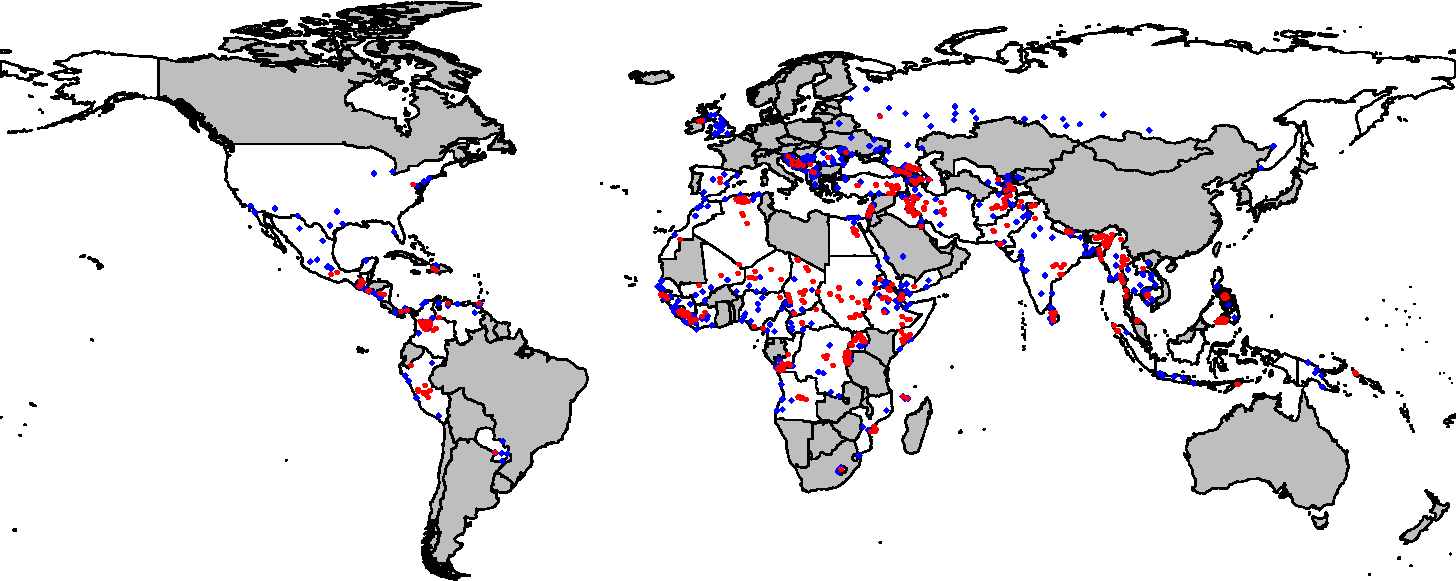
\includegraphics[width=1\textwidth]{CityConfMap-crop}
	\caption{This map illustrates the geographic distribution of all internal armed conflicts and major cities from 1989 to 2008. Countries for which no armed conflicts are recorded are shaded in grey.}
	\label{fig:CityConfMap}
\end{amssidewaysfigure}
\FloatBarrier

Using our geo-referenced conflict and urban center data, we proceed to compute the proximity of every civil armed conflict in a country-year from every urban center listed in that year.\footnote{Distances between centroid locations were computed using an iterative method of distance calculation proposed by \citet{vincenty:1975}.} Since our unit of analysis is the country-year, we aggregate the distance between conflicts and major cities by calculating the minimum logged distance any conflict is from a major city. For example, if a country faces four conflicts in a year, the datapoint for that country-year would be the minimum distance any conflict centroid is from any city centroid. In addition to identifying the minimum distance a conflict is from any city, we also create a variable that measures minimum distance of any conflict from the capital of the country. Given the importance of cities as drivers of macroeconomic growth the proximity of conflict to even one city should have at least a noticeable short-term impact on growth. Thus this choice of aggregation conforms clostest to our theoretical claims about how macroeconomic growth can be severely disrupted in cases where conflicts are proximate to major cities. 

Figure \ref{fig:distGdp} provides a cursory illustration of the relationship between GDP growth and our spatial proximity variables. Each bar on the rightmost panel represents the average GDP growth rate across country-years for which the minimum distance between the centroid of the conflict and capital city fell within a certain quartile range across our full sample. Clearly, as the minimum distance from a conflict to capital city declines, there is a sharp decline in average growth rates for the following year. On the rightmost panel of this figure, the same relationship holds when we test the effect of the minimum distance of conflict from any major urban center. 

\begin{figure}
	\centering
	\resizebox{.8\textwidth}{!}{% Created by tikzDevice version 0.7.0 on 2014-10-06 19:44:25
% !TEX encoding = UTF-8 Unicode
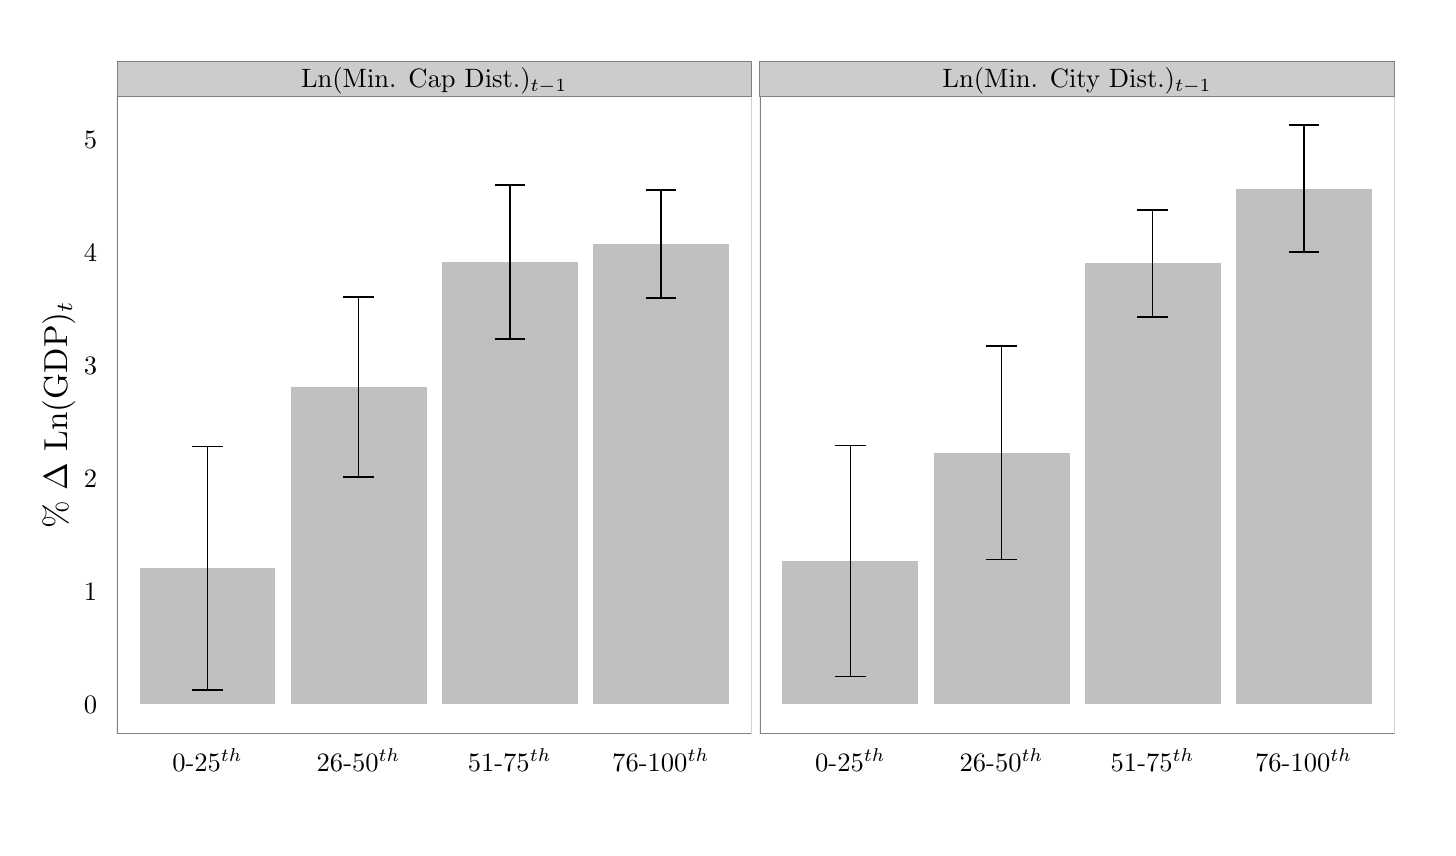
\begin{tikzpicture}[x=1pt,y=1pt]
\definecolor[named]{fillColor}{rgb}{1.00,1.00,1.00}
\path[use as bounding box,fill=fillColor,fill opacity=0.00] (0,0) rectangle (505.89,289.08);
\begin{scope}
\path[clip] (  0.00,  0.00) rectangle (505.89,289.08);
\definecolor[named]{drawColor}{rgb}{1.00,1.00,1.00}
\definecolor[named]{fillColor}{rgb}{1.00,1.00,1.00}

\path[draw=drawColor,line width= 0.6pt,line join=round,line cap=round,fill=fillColor] (  0.00,  0.00) rectangle (505.89,289.08);
\end{scope}
\begin{scope}
\path[clip] ( 32.22, 34.03) rectangle (261.53,264.40);
\definecolor[named]{fillColor}{rgb}{1.00,1.00,1.00}

\path[fill=fillColor] ( 32.22, 34.03) rectangle (261.53,264.40);
\definecolor[named]{fillColor}{rgb}{0.75,0.75,0.75}

\path[fill=fillColor] ( 40.41, 44.51) rectangle ( 89.55, 93.75);

\path[fill=fillColor] ( 95.01, 44.51) rectangle (144.14,159.24);

\path[fill=fillColor] (149.60, 44.51) rectangle (198.74,204.41);

\path[fill=fillColor] (204.20, 44.51) rectangle (253.34,210.90);
\definecolor[named]{drawColor}{rgb}{0.00,0.00,0.00}

\path[draw=drawColor,line width= 0.6pt,line join=round] ( 59.52,137.78) --
	( 70.44,137.78);

\path[draw=drawColor,line width= 0.6pt,line join=round] ( 64.98,137.78) --
	( 64.98, 49.72);

\path[draw=drawColor,line width= 0.6pt,line join=round] ( 59.52, 49.72) --
	( 70.44, 49.72);

\path[draw=drawColor,line width= 0.6pt,line join=round] (114.12,191.72) --
	(125.04,191.72);

\path[draw=drawColor,line width= 0.6pt,line join=round] (119.58,191.72) --
	(119.58,126.77);

\path[draw=drawColor,line width= 0.6pt,line join=round] (114.12,126.77) --
	(125.04,126.77);

\path[draw=drawColor,line width= 0.6pt,line join=round] (168.71,232.19) --
	(179.63,232.19);

\path[draw=drawColor,line width= 0.6pt,line join=round] (174.17,232.19) --
	(174.17,176.63);

\path[draw=drawColor,line width= 0.6pt,line join=round] (168.71,176.63) --
	(179.63,176.63);

\path[draw=drawColor,line width= 0.6pt,line join=round] (223.31,230.44) --
	(234.23,230.44);

\path[draw=drawColor,line width= 0.6pt,line join=round] (228.77,230.44) --
	(228.77,191.36);

\path[draw=drawColor,line width= 0.6pt,line join=round] (223.31,191.36) --
	(234.23,191.36);
\definecolor[named]{drawColor}{rgb}{0.50,0.50,0.50}

\path[draw=drawColor,line width= 0.6pt,line join=round,line cap=round] ( 32.22, 34.03) rectangle (261.53,264.40);
\end{scope}
\begin{scope}
\path[clip] (264.54, 34.03) rectangle (493.85,264.40);
\definecolor[named]{fillColor}{rgb}{1.00,1.00,1.00}

\path[fill=fillColor] (264.54, 34.03) rectangle (493.85,264.40);
\definecolor[named]{fillColor}{rgb}{0.75,0.75,0.75}

\path[fill=fillColor] (272.73, 44.51) rectangle (321.87, 96.35);

\path[fill=fillColor] (327.33, 44.51) rectangle (376.46,135.46);

\path[fill=fillColor] (381.92, 44.51) rectangle (431.06,203.89);

\path[fill=fillColor] (436.52, 44.51) rectangle (485.66,230.96);
\definecolor[named]{drawColor}{rgb}{0.00,0.00,0.00}

\path[draw=drawColor,line width= 0.6pt,line join=round] (291.84,138.07) --
	(302.76,138.07);

\path[draw=drawColor,line width= 0.6pt,line join=round] (297.30,138.07) --
	(297.30, 54.63);

\path[draw=drawColor,line width= 0.6pt,line join=round] (291.84, 54.63) --
	(302.76, 54.63);

\path[draw=drawColor,line width= 0.6pt,line join=round] (346.43,174.04) --
	(357.35,174.04);

\path[draw=drawColor,line width= 0.6pt,line join=round] (351.89,174.04) --
	(351.89, 96.87);

\path[draw=drawColor,line width= 0.6pt,line join=round] (346.43, 96.87) --
	(357.35, 96.87);

\path[draw=drawColor,line width= 0.6pt,line join=round] (401.03,223.16) --
	(411.95,223.16);

\path[draw=drawColor,line width= 0.6pt,line join=round] (406.49,223.16) --
	(406.49,184.61);

\path[draw=drawColor,line width= 0.6pt,line join=round] (401.03,184.61) --
	(411.95,184.61);

\path[draw=drawColor,line width= 0.6pt,line join=round] (455.63,253.93) --
	(466.55,253.93);

\path[draw=drawColor,line width= 0.6pt,line join=round] (461.09,253.93) --
	(461.09,208.00);

\path[draw=drawColor,line width= 0.6pt,line join=round] (455.63,208.00) --
	(466.55,208.00);
\definecolor[named]{drawColor}{rgb}{0.50,0.50,0.50}

\path[draw=drawColor,line width= 0.6pt,line join=round,line cap=round] (264.54, 34.03) rectangle (493.85,264.40);
\end{scope}
\begin{scope}
\path[clip] (  0.00,  0.00) rectangle (505.89,289.08);
\definecolor[named]{drawColor}{rgb}{0.50,0.50,0.50}
\definecolor[named]{fillColor}{rgb}{0.80,0.80,0.80}

\path[draw=drawColor,line width= 0.2pt,line join=round,line cap=round,fill=fillColor] ( 32.22,264.40) rectangle (261.53,277.04);
\definecolor[named]{drawColor}{rgb}{0.00,0.00,0.00}

\node[text=drawColor,anchor=base,inner sep=0pt, outer sep=0pt, scale=  0.96] at (146.87,267.41) {Ln(Min. Cap Dist.)$_{t-1}$};
\end{scope}
\begin{scope}
\path[clip] (  0.00,  0.00) rectangle (505.89,289.08);
\definecolor[named]{drawColor}{rgb}{0.50,0.50,0.50}
\definecolor[named]{fillColor}{rgb}{0.80,0.80,0.80}

\path[draw=drawColor,line width= 0.2pt,line join=round,line cap=round,fill=fillColor] (264.54,264.40) rectangle (493.85,277.04);
\definecolor[named]{drawColor}{rgb}{0.00,0.00,0.00}

\node[text=drawColor,anchor=base,inner sep=0pt, outer sep=0pt, scale=  0.96] at (379.19,267.41) {Ln(Min. City Dist.)$_{t-1}$};
\end{scope}
\begin{scope}
\path[clip] (  0.00,  0.00) rectangle (505.89,289.08);
\definecolor[named]{drawColor}{rgb}{0.00,0.00,0.00}

\node[text=drawColor,anchor=base east,inner sep=0pt, outer sep=0pt, scale=  0.96] at ( 25.11, 41.20) {0};

\node[text=drawColor,anchor=base east,inner sep=0pt, outer sep=0pt, scale=  0.96] at ( 25.11, 82.02) {1};

\node[text=drawColor,anchor=base east,inner sep=0pt, outer sep=0pt, scale=  0.96] at ( 25.11,122.84) {2};

\node[text=drawColor,anchor=base east,inner sep=0pt, outer sep=0pt, scale=  0.96] at ( 25.11,163.67) {3};

\node[text=drawColor,anchor=base east,inner sep=0pt, outer sep=0pt, scale=  0.96] at ( 25.11,204.49) {4};

\node[text=drawColor,anchor=base east,inner sep=0pt, outer sep=0pt, scale=  0.96] at ( 25.11,245.31) {5};
\end{scope}
\begin{scope}
\path[clip] (  0.00,  0.00) rectangle (505.89,289.08);
\definecolor[named]{drawColor}{rgb}{0.00,0.00,0.00}

\node[text=drawColor,anchor=base,inner sep=0pt, outer sep=0pt, scale=  0.96] at ( 64.98, 20.31) {0-25$^{th}$};

\node[text=drawColor,anchor=base,inner sep=0pt, outer sep=0pt, scale=  0.96] at (119.58, 20.31) {26-50$^{th}$};

\node[text=drawColor,anchor=base,inner sep=0pt, outer sep=0pt, scale=  0.96] at (174.17, 20.31) {51-75$^{th}$};

\node[text=drawColor,anchor=base,inner sep=0pt, outer sep=0pt, scale=  0.96] at (228.77, 20.31) {76-100$^{th}$};
\end{scope}
\begin{scope}
\path[clip] (  0.00,  0.00) rectangle (505.89,289.08);
\definecolor[named]{drawColor}{rgb}{0.00,0.00,0.00}

\node[text=drawColor,anchor=base,inner sep=0pt, outer sep=0pt, scale=  0.96] at (297.30, 20.31) {0-25$^{th}$};

\node[text=drawColor,anchor=base,inner sep=0pt, outer sep=0pt, scale=  0.96] at (351.89, 20.31) {26-50$^{th}$};

\node[text=drawColor,anchor=base,inner sep=0pt, outer sep=0pt, scale=  0.96] at (406.49, 20.31) {51-75$^{th}$};

\node[text=drawColor,anchor=base,inner sep=0pt, outer sep=0pt, scale=  0.96] at (461.09, 20.31) {76-100$^{th}$};
\end{scope}
\begin{scope}
\path[clip] (  0.00,  0.00) rectangle (505.89,289.08);
\definecolor[named]{drawColor}{rgb}{0.00,0.00,0.00}

\node[text=drawColor,rotate= 90.00,anchor=base,inner sep=0pt, outer sep=0pt, scale=  1.20] at ( 14.29,149.22) {\% $\Delta$ Ln(GDP)$_{t}$};
\end{scope}
\end{tikzpicture}
}
	\caption{Average percent change in GDP growth at time $t$ by distance from conflict to capital city on rightmost panel at time $t-1$, and from conflict to any city on the leftmost. The error bars represent the 95\% confidence interval around the mean.}
	\label{fig:distGdp}
\end{figure}

\subsection{Empirical Model}

Next, we move beyond this cursory illustration and explicate our full modeling strategy. Given how we constructed our spatial proximity of conflict variables, it would make little sense to include both within one model. The obvious problem we would run into is that there would be cases for which the minimum distance of a conflict to any city would be the same as the minimum distance to the capital. Thus we estimate two separate models, one where we include the minimum distance from a conflict to the capital and the other where we include the minimum distance to any urban center. In addition to the inclusion of our spatial proximity covariates we include a number of control measures to account for extant explanations of how civil war dynamics affect GDP growth and to mitigate omitted variable bias. 

From the PRIO Armed Conflict dataset we bring in additional information about conflict intensity, duration, the area covered by the conflict, and the number of conflicts \citep{themner:wallensteen:2014}. Conflict intensity is a binary that distinguishes between minor armed conflicts (between 25 and 999 annual battle deaths) and wars (at least 1000 annual battle deaths), and we set this equal to one if any of the conflicts in a country year were classified as a war and zero if not. In aggregating conflict duration to the country year level, we bring in the duration (measured in years) of the longest lasting conflict by a certain country-year. Conflict area measures the conflict zone in square kilometers. To include this in our country-year model, we sum up the area covered by each conflict being fought and divide by the total land area of the country. Finally, the number of conflicts is simply a count of the number of ongoing internal armed conflicts in a country-year according to the PRIO dataset.

% From this we then create a binary measure that is one if greater than 50\% of a country's total land area is immersed in conflict and zero otherwise. 

Aggregating each of the PRIO conflict descriptive measures in this way is to help account for those countries in which conflicts are especially intense, cover large areas, have been long-lasting, or are one of many ongoing conflicts. Given the findings in the extant literature, our expectation is that each of these measures should have a negative effect on economic growth. Though we also expect that the substantive implications of any one of these measures will matter less than the adverse effect to economic growth by the spatial proximity of conflict to urban centers.

We also include a number of variables that help to capture structural and institutional aspects of the country itself. First, we include a binary for whether the country is classified as upper income by the World Bank and for the level of inflation in the country. Second, we also control for the level of democracy in the country using the polity index \citep{marshall:etal:2013}. We also control for the proportion of a country's GDP that is made up of natural resource rents. This is a particularly important variable to control for as countries that draw a large share of their GDP from natural resource rents likely rely less on urban centers to serve as drivers of growth. Finally, given that the timeframe of our sample overlaps with the occurrence of two major global economic crises, the 1997 Asian financial crisis and the 2008 financial crisis, we add a control for the average GDP growth across all countries in the world. 

To estimate variation in growth rates, we use a random effects model clustered on countries. A random effects specification is preferred to using fixed effects here as we are not interested in estimating the change in GDP within units over time, rather our purpose is to explain variation between units. However, to ensure that it is also statistically justifiable to make this choice we run a Hausman specification test \citep{greene:2008}. For both the minimum conflict distance to any and to capital city specifications we fail to reject the null hypothesis at either the 90 and 95\% confidence intervals, providing at least some initial evidence that we are justified in our choice. However, as \citet{clark:linzer:2015} note not finding a significant difference through the Hausman test does not necessarily mean ``that the random effects is `safely` free from bias, and therefore to be preferred over the fixed effects estimator'' (pg., 2). We utilize their more nuanced typology for further arbitrating between fixed and random effects, and again we find that random effects are preferred in this case.\footnote{A lengthier discussion of the \citet{clark:linzer:2015} procedure and its application to our data can be found in the Appendix.}

The total number of observations we have for this analysis are 497 country-year cases of civil war from 68 different countries during the period of 1989 to 2008. The estimation model is shown below, where $Ln(Min. \; Conflict \; Dist.)_{i,t-1}$ is a placeholder for $Ln(Min. \; Capital \; Dist.)_{i,t-1}$ and $Ln(Min. \; City \; Dist.)_{i,t-1}$:

\begin{align*}
	\% \Delta GDP_{i,t} &= \beta_{1}(Ln(Min. \; Conflict \; Dist.)_{i,t-1}) \\
	& \;+\; \beta_{2}(Conflict \; Intensity_{i,t-1}) \;+\; \beta_{3}(Conflict \; Duration_{i,t-1}) \\
	& \;+\; \beta_{4}(Conflict \; Area_{i,t-1} \;/\; Land \; Area_{i,t-1}) \\
	& \;+\; \beta_{5}(Number \; of \; Conflicts_{i,t-1}) \;+\; \beta_{6}(Upper \; Income_{i,t}) \\	
	& \;+\; \beta_{7}(Inflation_{i,t-1}) \;+\; \beta_{8}(Democracy_{i,t-1}) \\
	& \;+\; \beta_{9}(Resource \; Rents/GDP_{t-1}) \;+\; \beta_{10}(World \; GDP \; Growth_{t})
\end{align*}

\subsection{Baseline Model}

Before we move to discussing the results of the model specification that we have described above we estimate a simple, baseline model to assess the effect of any civil conflict on growth. For this model we use a specification as similar as possible to the one we explicated in the previous section, with the key difference being that this baseline model is estimated using a full country-year panel with fixed effects.\footnote{In choosing between fixed and random effects, we again followed the typology set out by \citet{clark:linzer:2015}, and, in this case, found that the fixed effects specification was preferred.} The dependent variable is again annual percent change in GDP from the World Development Indicators, and the key independent variable here is whether or not the country was engaged in a civil war in the previous year according to the PRIO Armed Conflict dataset. Since we are using a full country-year panel, we have to omit the PRIO conflict specific variables (e.g., conflict intensity, conflict duration) as they are undefined for country-year observations in which no conflict was taking place. The rest of the independent variables are similar to the model specified in the previous section, specifically, we include: whether or not the country is classified as upper income, lagged version of inflation, lagged version of polity, lagged version of resource rents as a proportion of GDP, and average GDP growth across all countries in the world. 

% \begin{align*}
% 	\% \Delta GDP_{i,t} &= \beta_{1}(Civil\;War_{i,t-1}) \\
% 	& \;+\; \beta_{6}(Upper \; Income_{i,t}) \;+\; \beta_{7}(Inflation_{i,t-1}) \\	
% 	& \;+\; \beta_{8}(Democracy_{i,t-1}) \;+\; \beta_{9}(Resource \; Rents/GDP_{t-1}) \\
% 	& \;+\; \beta_{10}(World \; GDP \; Growth_{t})
% \end{align*}

We will eschew discussing the controls since the primary purpose of this analysis is to determine a baseline effect for civil war. Additionally, for the sake of space we do not show the full results from this regression, but they are available in section \ref{baseline} of the Appendix. The key result pertains to the civil war variable, the $\beta$ estimate is approximately -1.011 with a standard error of 0.521. 

To assess the substantive significance of this variable we turn to a simulation based analysis. To to do this we set up two scenarios, one in which a civil war occurred and in the other no civil war, all the other parameters were set to their median value. Next, we conduct 1,000 random draws from a multivariate normal to obtain a distribution of point estimates of each regression coefficient. Last, we simply matrix multiply the draws from the multivariate normal with the transposed scenario matrix to obtain expected values of GDP growth by the two scenarios. The resulting distributions are shown in figure \ref{fig:civWarEffect}. 

\begin{figure}
	\centering
	\resizebox{.45\textwidth}{!}{% Created by tikzDevice version 0.7.0 on 2015-08-25 22:05:25
% !TEX encoding = UTF-8 Unicode
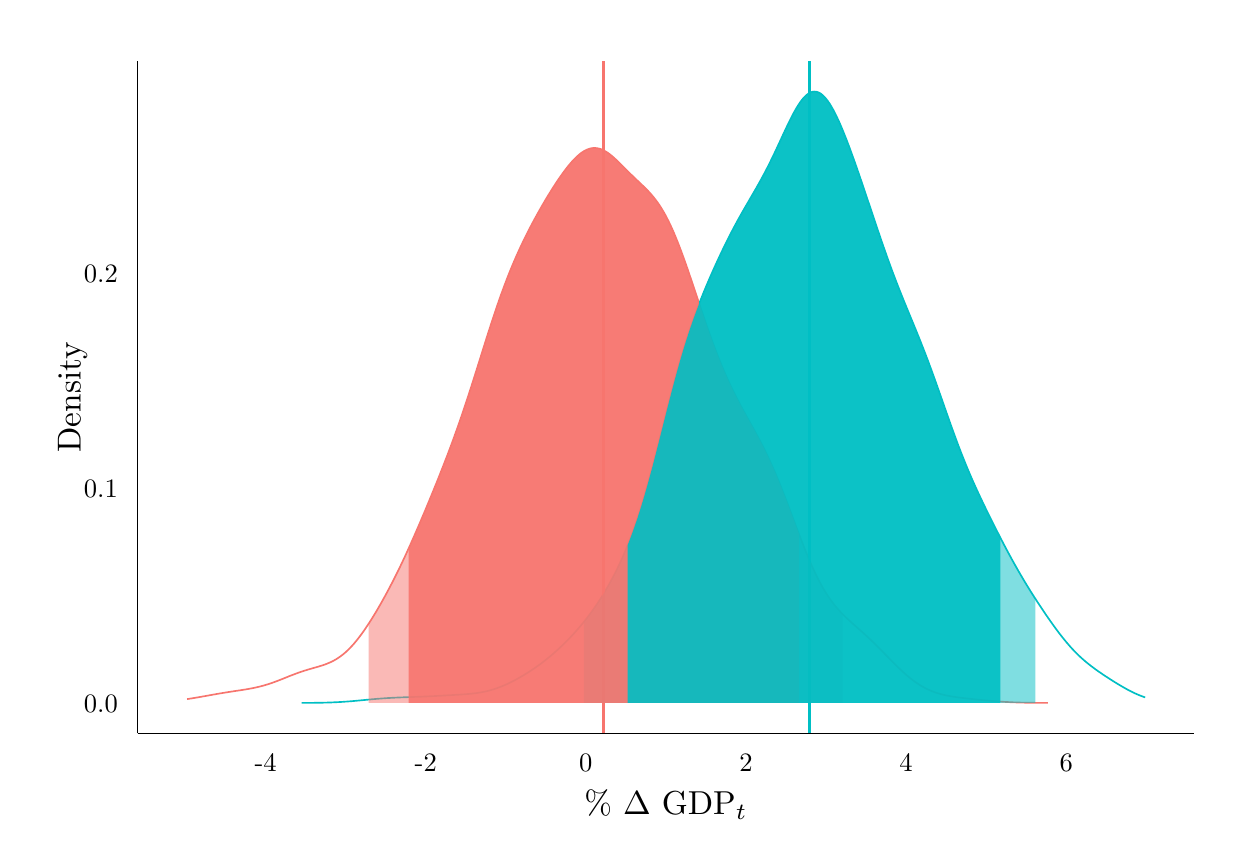
\begin{tikzpicture}[x=1pt,y=1pt]
\definecolor[named]{fillColor}{rgb}{1.00,1.00,1.00}
\path[use as bounding box,fill=fillColor,fill opacity=0.00] (0,0) rectangle (433.62,289.08);
\begin{scope}
\path[clip] (  0.00,  0.00) rectangle (433.62,289.08);
\definecolor[named]{drawColor}{rgb}{1.00,1.00,1.00}
\definecolor[named]{fillColor}{rgb}{1.00,1.00,1.00}

\path[draw=drawColor,line width= 0.6pt,line join=round,line cap=round,fill=fillColor] (  0.00,  0.00) rectangle (433.62,289.08);
\end{scope}
\begin{scope}
\path[clip] ( 39.69, 34.03) rectangle (421.57,277.03);
\definecolor[named]{fillColor}{rgb}{1.00,1.00,1.00}

\path[fill=fillColor] ( 39.69, 34.03) rectangle (421.57,277.03);
\definecolor[named]{drawColor}{rgb}{0.97,0.46,0.43}

\path[draw=drawColor,line width= 0.6pt,line join=round] ( 57.61, 46.46) --
	( 58.27, 46.56) --
	( 58.92, 46.66) --
	( 59.58, 46.77) --
	( 60.24, 46.88) --
	( 60.89, 46.99) --
	( 61.55, 47.10) --
	( 62.20, 47.21) --
	( 62.86, 47.33) --
	( 63.52, 47.45) --
	( 64.17, 47.56) --
	( 64.83, 47.68) --
	( 65.48, 47.80) --
	( 66.14, 47.92) --
	( 66.80, 48.04) --
	( 67.45, 48.15) --
	( 68.11, 48.27) --
	( 68.77, 48.38) --
	( 69.42, 48.49) --
	( 70.08, 48.60) --
	( 70.73, 48.71) --
	( 71.39, 48.82) --
	( 72.05, 48.92) --
	( 72.70, 49.03) --
	( 73.36, 49.13) --
	( 74.01, 49.23) --
	( 74.67, 49.33) --
	( 75.33, 49.43) --
	( 75.98, 49.52) --
	( 76.64, 49.62) --
	( 77.30, 49.72) --
	( 77.95, 49.83) --
	( 78.61, 49.93) --
	( 79.26, 50.04) --
	( 79.92, 50.16) --
	( 80.58, 50.28) --
	( 81.23, 50.40) --
	( 81.89, 50.54) --
	( 82.54, 50.68) --
	( 83.20, 50.83) --
	( 83.86, 50.99) --
	( 84.51, 51.16) --
	( 85.17, 51.33) --
	( 85.82, 51.52) --
	( 86.48, 51.72) --
	( 87.14, 51.93) --
	( 87.79, 52.15) --
	( 88.45, 52.37) --
	( 89.11, 52.61) --
	( 89.76, 52.85) --
	( 90.42, 53.10) --
	( 91.07, 53.35) --
	( 91.73, 53.61) --
	( 92.39, 53.88) --
	( 93.04, 54.14) --
	( 93.70, 54.40) --
	( 94.35, 54.67) --
	( 95.01, 54.93) --
	( 95.67, 55.18) --
	( 96.32, 55.43) --
	( 96.98, 55.68) --
	( 97.64, 55.92) --
	( 98.29, 56.15) --
	( 98.95, 56.37) --
	( 99.60, 56.59) --
	(100.26, 56.80) --
	(100.92, 57.00) --
	(101.57, 57.20) --
	(102.23, 57.39) --
	(102.88, 57.58) --
	(103.54, 57.77) --
	(104.20, 57.95) --
	(104.85, 58.14) --
	(105.51, 58.34) --
	(106.17, 58.55) --
	(106.82, 58.76) --
	(107.48, 58.99) --
	(108.13, 59.24) --
	(108.79, 59.51) --
	(109.45, 59.80) --
	(110.10, 60.12) --
	(110.76, 60.46) --
	(111.41, 60.83) --
	(112.07, 61.24) --
	(112.73, 61.69) --
	(113.38, 62.17) --
	(114.04, 62.68) --
	(114.70, 63.23) --
	(115.35, 63.83) --
	(116.01, 64.46) --
	(116.66, 65.13) --
	(117.32, 65.83) --
	(117.98, 66.57) --
	(118.63, 67.36) --
	(119.29, 68.17) --
	(119.94, 69.02) --
	(120.60, 69.90) --
	(121.26, 70.81) --
	(121.91, 71.75) --
	(122.57, 72.73) --
	(123.22, 73.72) --
	(123.88, 74.74) --
	(124.54, 75.78) --
	(125.19, 76.85) --
	(125.85, 77.94) --
	(126.51, 79.05) --
	(127.16, 80.18) --
	(127.82, 81.33) --
	(128.47, 82.50) --
	(129.13, 83.69) --
	(129.79, 84.90) --
	(130.44, 86.13) --
	(131.10, 87.38) --
	(131.75, 88.64) --
	(132.41, 89.93) --
	(133.07, 91.23) --
	(133.72, 92.56) --
	(134.38, 93.90) --
	(135.04, 95.26) --
	(135.69, 96.64) --
	(136.35, 98.04) --
	(137.00, 99.46) --
	(137.66,100.90) --
	(138.32,102.35) --
	(138.97,103.82) --
	(139.63,105.30) --
	(140.28,106.80) --
	(140.94,108.31) --
	(141.60,109.83) --
	(142.25,111.37) --
	(142.91,112.92) --
	(143.57,114.47) --
	(144.22,116.04) --
	(144.88,117.62) --
	(145.53,119.21) --
	(146.19,120.80) --
	(146.85,122.41) --
	(147.50,124.03) --
	(148.16,125.66) --
	(148.81,127.30) --
	(149.47,128.96) --
	(150.13,130.63) --
	(150.78,132.32) --
	(151.44,134.02) --
	(152.10,135.75) --
	(152.75,137.49) --
	(153.41,139.26) --
	(154.06,141.06) --
	(154.72,142.88) --
	(155.38,144.72) --
	(156.03,146.59) --
	(156.69,148.49) --
	(157.34,150.41) --
	(158.00,152.37) --
	(158.66,154.34) --
	(159.31,156.34) --
	(159.97,158.37) --
	(160.62,160.41) --
	(161.28,162.47) --
	(161.94,164.55) --
	(162.59,166.63) --
	(163.25,168.73) --
	(163.91,170.82) --
	(164.56,172.91) --
	(165.22,175.00) --
	(165.87,177.07) --
	(166.53,179.13) --
	(167.19,181.17) --
	(167.84,183.18) --
	(168.50,185.17) --
	(169.15,187.12) --
	(169.81,189.05) --
	(170.47,190.93) --
	(171.12,192.77) --
	(171.78,194.57) --
	(172.44,196.34) --
	(173.09,198.06) --
	(173.75,199.74) --
	(174.40,201.37) --
	(175.06,202.96) --
	(175.72,204.52) --
	(176.37,206.03) --
	(177.03,207.51) --
	(177.68,208.95) --
	(178.34,210.36) --
	(179.00,211.74) --
	(179.65,213.09) --
	(180.31,214.41) --
	(180.97,215.70) --
	(181.62,216.97) --
	(182.28,218.22) --
	(182.93,219.45) --
	(183.59,220.65) --
	(184.25,221.84) --
	(184.90,223.01) --
	(185.56,224.16) --
	(186.21,225.30) --
	(186.87,226.42) --
	(187.53,227.52) --
	(188.18,228.61) --
	(188.84,229.67) --
	(189.49,230.72) --
	(190.15,231.75) --
	(190.81,232.77) --
	(191.46,233.75) --
	(192.12,234.72) --
	(192.78,235.66) --
	(193.43,236.58) --
	(194.09,237.47) --
	(194.74,238.33) --
	(195.40,239.15) --
	(196.06,239.94) --
	(196.71,240.70) --
	(197.37,241.41) --
	(198.02,242.07) --
	(198.68,242.69) --
	(199.34,243.25) --
	(199.99,243.77) --
	(200.65,244.23) --
	(201.31,244.62) --
	(201.96,244.95) --
	(202.62,245.21) --
	(203.27,245.41) --
	(203.93,245.55) --
	(204.59,245.61) --
	(205.24,245.59) --
	(205.90,245.51) --
	(206.55,245.36) --
	(207.21,245.15) --
	(207.87,244.88) --
	(208.52,244.54) --
	(209.18,244.14) --
	(209.84,243.70) --
	(210.49,243.21) --
	(211.15,242.68) --
	(211.80,242.11) --
	(212.46,241.51) --
	(213.12,240.89) --
	(213.77,240.26) --
	(214.43,239.61) --
	(215.08,238.95) --
	(215.74,238.29) --
	(216.40,237.64) --
	(217.05,236.98) --
	(217.71,236.34) --
	(218.37,235.69) --
	(219.02,235.06) --
	(219.68,234.44) --
	(220.33,233.82) --
	(220.99,233.19) --
	(221.65,232.57) --
	(222.30,231.94) --
	(222.96,231.30) --
	(223.61,230.65) --
	(224.27,229.97) --
	(224.93,229.26) --
	(225.58,228.51) --
	(226.24,227.72) --
	(226.89,226.88) --
	(227.55,226.00) --
	(228.21,225.06) --
	(228.86,224.05) --
	(229.52,222.97) --
	(230.18,221.82) --
	(230.83,220.61) --
	(231.49,219.33) --
	(232.14,217.99) --
	(232.80,216.55) --
	(233.46,215.06) --
	(234.11,213.50) --
	(234.77,211.88) --
	(235.42,210.21) --
	(236.08,208.48) --
	(236.74,206.69) --
	(237.39,204.87) --
	(238.05,203.01) --
	(238.71,201.12) --
	(239.36,199.20) --
	(240.02,197.26) --
	(240.67,195.30) --
	(241.33,193.34) --
	(241.99,191.38) --
	(242.64,189.42) --
	(243.30,187.47) --
	(243.95,185.53) --
	(244.61,183.61) --
	(245.27,181.71) --
	(245.92,179.83) --
	(246.58,177.99) --
	(247.24,176.18) --
	(247.89,174.40) --
	(248.55,172.66) --
	(249.20,170.95) --
	(249.86,169.29) --
	(250.52,167.67) --
	(251.17,166.09) --
	(251.83,164.55) --
	(252.48,163.05) --
	(253.14,161.59) --
	(253.80,160.18) --
	(254.45,158.80) --
	(255.11,157.45) --
	(255.77,156.14) --
	(256.42,154.86) --
	(257.08,153.60) --
	(257.73,152.37) --
	(258.39,151.16) --
	(259.05,149.96) --
	(259.70,148.78) --
	(260.36,147.60) --
	(261.01,146.42) --
	(261.67,145.25) --
	(262.33,144.06) --
	(262.98,142.87) --
	(263.64,141.66) --
	(264.29,140.43) --
	(264.95,139.18) --
	(265.61,137.90) --
	(266.26,136.60) --
	(266.92,135.26) --
	(267.58,133.89) --
	(268.23,132.48) --
	(268.89,131.03) --
	(269.54,129.56) --
	(270.20,128.04) --
	(270.86,126.48) --
	(271.51,124.89) --
	(272.17,123.27) --
	(272.82,121.61) --
	(273.48,119.94) --
	(274.14,118.23) --
	(274.79,116.50) --
	(275.45,114.77) --
	(276.11,113.02) --
	(276.76,111.27) --
	(277.42,109.51) --
	(278.07,107.77) --
	(278.73,106.04) --
	(279.39,104.32) --
	(280.04,102.63) --
	(280.70,100.96) --
	(281.35, 99.34) --
	(282.01, 97.75) --
	(282.67, 96.20) --
	(283.32, 94.70) --
	(283.98, 93.24) --
	(284.64, 91.85) --
	(285.29, 90.51) --
	(285.95, 89.22) --
	(286.60, 87.98) --
	(287.26, 86.80) --
	(287.92, 85.69) --
	(288.57, 84.63) --
	(289.23, 83.62) --
	(289.88, 82.66) --
	(290.54, 81.75) --
	(291.20, 80.88) --
	(291.85, 80.07) --
	(292.51, 79.29) --
	(293.17, 78.55) --
	(293.82, 77.84) --
	(294.48, 77.16) --
	(295.13, 76.51) --
	(295.79, 75.87) --
	(296.45, 75.26) --
	(297.10, 74.66) --
	(297.76, 74.06) --
	(298.41, 73.48) --
	(299.07, 72.90) --
	(299.73, 72.32) --
	(300.38, 71.74) --
	(301.04, 71.16) --
	(301.69, 70.58) --
	(302.35, 69.98) --
	(303.01, 69.38) --
	(303.66, 68.78) --
	(304.32, 68.16) --
	(304.98, 67.53) --
	(305.63, 66.90) --
	(306.29, 66.26) --
	(306.94, 65.61) --
	(307.60, 64.95) --
	(308.26, 64.29) --
	(308.91, 63.62) --
	(309.57, 62.95) --
	(310.22, 62.28) --
	(310.88, 61.61) --
	(311.54, 60.93) --
	(312.19, 60.27) --
	(312.85, 59.60) --
	(313.51, 58.95) --
	(314.16, 58.30) --
	(314.82, 57.66) --
	(315.47, 57.04) --
	(316.13, 56.43) --
	(316.79, 55.83) --
	(317.44, 55.25) --
	(318.10, 54.69) --
	(318.75, 54.15) --
	(319.41, 53.63) --
	(320.07, 53.13) --
	(320.72, 52.65) --
	(321.38, 52.20) --
	(322.04, 51.76) --
	(322.69, 51.35) --
	(323.35, 50.97) --
	(324.00, 50.61) --
	(324.66, 50.26) --
	(325.32, 49.94) --
	(325.97, 49.65) --
	(326.63, 49.37) --
	(327.28, 49.12) --
	(327.94, 48.88) --
	(328.60, 48.66) --
	(329.25, 48.46) --
	(329.91, 48.28) --
	(330.56, 48.11) --
	(331.22, 47.95) --
	(331.88, 47.80) --
	(332.53, 47.67) --
	(333.19, 47.55) --
	(333.85, 47.43) --
	(334.50, 47.33) --
	(335.16, 47.23) --
	(335.81, 47.13) --
	(336.47, 47.04) --
	(337.13, 46.96) --
	(337.78, 46.88) --
	(338.44, 46.80) --
	(339.09, 46.72) --
	(339.75, 46.65) --
	(340.41, 46.58) --
	(341.06, 46.51) --
	(341.72, 46.44) --
	(342.38, 46.37) --
	(343.03, 46.30) --
	(343.69, 46.23) --
	(344.34, 46.17) --
	(345.00, 46.10) --
	(345.66, 46.04) --
	(346.31, 45.98) --
	(346.97, 45.92) --
	(347.62, 45.86) --
	(348.28, 45.80) --
	(348.94, 45.75) --
	(349.59, 45.69) --
	(350.25, 45.64) --
	(350.91, 45.59) --
	(351.56, 45.55) --
	(352.22, 45.50) --
	(352.87, 45.46) --
	(353.53, 45.42) --
	(354.19, 45.39) --
	(354.84, 45.35) --
	(355.50, 45.32) --
	(356.15, 45.29) --
	(356.81, 45.27) --
	(357.47, 45.24) --
	(358.12, 45.22) --
	(358.78, 45.20) --
	(359.44, 45.19) --
	(360.09, 45.17) --
	(360.75, 45.16) --
	(361.40, 45.14) --
	(362.06, 45.13) --
	(362.72, 45.12) --
	(363.37, 45.12) --
	(364.03, 45.11) --
	(364.68, 45.10) --
	(365.34, 45.10) --
	(366.00, 45.09) --
	(366.65, 45.09) --
	(367.31, 45.09) --
	(367.96, 45.08) --
	(368.62, 45.08);
\definecolor[named]{drawColor}{rgb}{0.00,0.75,0.77}

\path[draw=drawColor,line width= 0.6pt,line join=round] ( 98.99, 45.08) --
	( 99.62, 45.08) --
	(100.25, 45.09) --
	(100.88, 45.09) --
	(101.51, 45.09) --
	(102.14, 45.10) --
	(102.77, 45.10) --
	(103.40, 45.11) --
	(104.03, 45.12) --
	(104.66, 45.13) --
	(105.29, 45.14) --
	(105.92, 45.15) --
	(106.55, 45.16) --
	(107.18, 45.18) --
	(107.81, 45.19) --
	(108.44, 45.21) --
	(109.07, 45.23) --
	(109.70, 45.25) --
	(110.33, 45.28) --
	(110.95, 45.31) --
	(111.58, 45.34) --
	(112.21, 45.37) --
	(112.84, 45.40) --
	(113.47, 45.44) --
	(114.10, 45.48) --
	(114.73, 45.53) --
	(115.36, 45.57) --
	(115.99, 45.62) --
	(116.62, 45.67) --
	(117.25, 45.72) --
	(117.88, 45.78) --
	(118.51, 45.83) --
	(119.14, 45.89) --
	(119.77, 45.95) --
	(120.40, 46.01) --
	(121.03, 46.07) --
	(121.66, 46.13) --
	(122.29, 46.19) --
	(122.92, 46.25) --
	(123.55, 46.31) --
	(124.18, 46.37) --
	(124.81, 46.43) --
	(125.44, 46.48) --
	(126.07, 46.54) --
	(126.70, 46.59) --
	(127.33, 46.64) --
	(127.96, 46.69) --
	(128.59, 46.73) --
	(129.22, 46.78) --
	(129.85, 46.82) --
	(130.48, 46.86) --
	(131.11, 46.89) --
	(131.74, 46.93) --
	(132.37, 46.96) --
	(133.00, 46.99) --
	(133.63, 47.02) --
	(134.26, 47.05) --
	(134.89, 47.07) --
	(135.52, 47.09) --
	(136.14, 47.12) --
	(136.77, 47.14) --
	(137.40, 47.16) --
	(138.03, 47.18) --
	(138.66, 47.20) --
	(139.29, 47.22) --
	(139.92, 47.25) --
	(140.55, 47.27) --
	(141.18, 47.29) --
	(141.81, 47.32) --
	(142.44, 47.34) --
	(143.07, 47.37) --
	(143.70, 47.40) --
	(144.33, 47.43) --
	(144.96, 47.46) --
	(145.59, 47.49) --
	(146.22, 47.52) --
	(146.85, 47.55) --
	(147.48, 47.59) --
	(148.11, 47.62) --
	(148.74, 47.65) --
	(149.37, 47.69) --
	(150.00, 47.72) --
	(150.63, 47.76) --
	(151.26, 47.80) --
	(151.89, 47.83) --
	(152.52, 47.87) --
	(153.15, 47.90) --
	(153.78, 47.94) --
	(154.41, 47.98) --
	(155.04, 48.02) --
	(155.67, 48.05) --
	(156.30, 48.09) --
	(156.93, 48.14) --
	(157.56, 48.18) --
	(158.19, 48.23) --
	(158.82, 48.28) --
	(159.45, 48.33) --
	(160.08, 48.39) --
	(160.71, 48.46) --
	(161.33, 48.53) --
	(161.96, 48.61) --
	(162.59, 48.70) --
	(163.22, 48.80) --
	(163.85, 48.91) --
	(164.48, 49.02) --
	(165.11, 49.15) --
	(165.74, 49.29) --
	(166.37, 49.44) --
	(167.00, 49.61) --
	(167.63, 49.78) --
	(168.26, 49.97) --
	(168.89, 50.17) --
	(169.52, 50.39) --
	(170.15, 50.62) --
	(170.78, 50.86) --
	(171.41, 51.11) --
	(172.04, 51.37) --
	(172.67, 51.65) --
	(173.30, 51.93) --
	(173.93, 52.23) --
	(174.56, 52.54) --
	(175.19, 52.86) --
	(175.82, 53.18) --
	(176.45, 53.52) --
	(177.08, 53.86) --
	(177.71, 54.22) --
	(178.34, 54.58) --
	(178.97, 54.95) --
	(179.60, 55.33) --
	(180.23, 55.72) --
	(180.86, 56.11) --
	(181.49, 56.52) --
	(182.12, 56.93) --
	(182.75, 57.35) --
	(183.38, 57.78) --
	(184.01, 58.23) --
	(184.64, 58.68) --
	(185.27, 59.14) --
	(185.89, 59.61) --
	(186.52, 60.09) --
	(187.15, 60.59) --
	(187.78, 61.09) --
	(188.41, 61.60) --
	(189.04, 62.13) --
	(189.67, 62.66) --
	(190.30, 63.21) --
	(190.93, 63.77) --
	(191.56, 64.34) --
	(192.19, 64.92) --
	(192.82, 65.51) --
	(193.45, 66.12) --
	(194.08, 66.73) --
	(194.71, 67.36) --
	(195.34, 68.00) --
	(195.97, 68.65) --
	(196.60, 69.32) --
	(197.23, 70.00) --
	(197.86, 70.69) --
	(198.49, 71.40) --
	(199.12, 72.13) --
	(199.75, 72.87) --
	(200.38, 73.62) --
	(201.01, 74.40) --
	(201.64, 75.19) --
	(202.27, 76.00) --
	(202.90, 76.83) --
	(203.53, 77.69) --
	(204.16, 78.56) --
	(204.79, 79.46) --
	(205.42, 80.37) --
	(206.05, 81.31) --
	(206.68, 82.27) --
	(207.31, 83.26) --
	(207.94, 84.28) --
	(208.57, 85.32) --
	(209.20, 86.39) --
	(209.83, 87.48) --
	(210.46, 88.61) --
	(211.08, 89.77) --
	(211.71, 90.96) --
	(212.34, 92.19) --
	(212.97, 93.45) --
	(213.60, 94.76) --
	(214.23, 96.11) --
	(214.86, 97.50) --
	(215.49, 98.94) --
	(216.12,100.42) --
	(216.75,101.96) --
	(217.38,103.56) --
	(218.01,105.21) --
	(218.64,106.92) --
	(219.27,108.69) --
	(219.90,110.51) --
	(220.53,112.41) --
	(221.16,114.37) --
	(221.79,116.39) --
	(222.42,118.47) --
	(223.05,120.61) --
	(223.68,122.81) --
	(224.31,125.07) --
	(224.94,127.37) --
	(225.57,129.72) --
	(226.20,132.11) --
	(226.83,134.53) --
	(227.46,136.99) --
	(228.09,139.47) --
	(228.72,141.96) --
	(229.35,144.46) --
	(229.98,146.96) --
	(230.61,149.45) --
	(231.24,151.93) --
	(231.87,154.38) --
	(232.50,156.81) --
	(233.13,159.21) --
	(233.76,161.57) --
	(234.39,163.88) --
	(235.02,166.14) --
	(235.64,168.36) --
	(236.27,170.52) --
	(236.90,172.63) --
	(237.53,174.67) --
	(238.16,176.66) --
	(238.79,178.60) --
	(239.42,180.49) --
	(240.05,182.32) --
	(240.68,184.10) --
	(241.31,185.83) --
	(241.94,187.52) --
	(242.57,189.17) --
	(243.20,190.78) --
	(243.83,192.35) --
	(244.46,193.89) --
	(245.09,195.41) --
	(245.72,196.90) --
	(246.35,198.36) --
	(246.98,199.80) --
	(247.61,201.22) --
	(248.24,202.62) --
	(248.87,204.00) --
	(249.50,205.37) --
	(250.13,206.72) --
	(250.76,208.05) --
	(251.39,209.36) --
	(252.02,210.65) --
	(252.65,211.93) --
	(253.28,213.19) --
	(253.91,214.42) --
	(254.54,215.64) --
	(255.17,216.83) --
	(255.80,218.01) --
	(256.43,219.17) --
	(257.06,220.31) --
	(257.69,221.44) --
	(258.32,222.55) --
	(258.95,223.65) --
	(259.58,224.74) --
	(260.21,225.82) --
	(260.83,226.90) --
	(261.46,227.98) --
	(262.09,229.06) --
	(262.72,230.15) --
	(263.35,231.24) --
	(263.98,232.36) --
	(264.61,233.48) --
	(265.24,234.63) --
	(265.87,235.80) --
	(266.50,236.98) --
	(267.13,238.20) --
	(267.76,239.44) --
	(268.39,240.71) --
	(269.02,242.00) --
	(269.65,243.30) --
	(270.28,244.63) --
	(270.91,245.98) --
	(271.54,247.34) --
	(272.17,248.70) --
	(272.80,250.06) --
	(273.43,251.42) --
	(274.06,252.76) --
	(274.69,254.08) --
	(275.32,255.38) --
	(275.95,256.63) --
	(276.58,257.85) --
	(277.21,259.00) --
	(277.84,260.09) --
	(278.47,261.11) --
	(279.10,262.06) --
	(279.73,262.92) --
	(280.36,263.68) --
	(280.99,264.34) --
	(281.62,264.89) --
	(282.25,265.34) --
	(282.88,265.69) --
	(283.51,265.90) --
	(284.14,265.99) --
	(284.77,265.96) --
	(285.39,265.82) --
	(286.02,265.56) --
	(286.65,265.19) --
	(287.28,264.67) --
	(287.91,264.05) --
	(288.54,263.33) --
	(289.17,262.51) --
	(289.80,261.59) --
	(290.43,260.56) --
	(291.06,259.44) --
	(291.69,258.24) --
	(292.32,256.97) --
	(292.95,255.63) --
	(293.58,254.22) --
	(294.21,252.74) --
	(294.84,251.22) --
	(295.47,249.64) --
	(296.10,248.02) --
	(296.73,246.37) --
	(297.36,244.66) --
	(297.99,242.93) --
	(298.62,241.18) --
	(299.25,239.40) --
	(299.88,237.59) --
	(300.51,235.77) --
	(301.14,233.93) --
	(301.77,232.07) --
	(302.40,230.21) --
	(303.03,228.33) --
	(303.66,226.45) --
	(304.29,224.57) --
	(304.92,222.69) --
	(305.55,220.81) --
	(306.18,218.93) --
	(306.81,217.06) --
	(307.44,215.20) --
	(308.07,213.35) --
	(308.70,211.52) --
	(309.33,209.71) --
	(309.96,207.91) --
	(310.58,206.14) --
	(311.21,204.39) --
	(311.84,202.67) --
	(312.47,200.96) --
	(313.10,199.29) --
	(313.73,197.64) --
	(314.36,196.01) --
	(314.99,194.41) --
	(315.62,192.82) --
	(316.25,191.25) --
	(316.88,189.70) --
	(317.51,188.17) --
	(318.14,186.64) --
	(318.77,185.11) --
	(319.40,183.59) --
	(320.03,182.07) --
	(320.66,180.53) --
	(321.29,178.99) --
	(321.92,177.43) --
	(322.55,175.86) --
	(323.18,174.27) --
	(323.81,172.66) --
	(324.44,171.03) --
	(325.07,169.37) --
	(325.70,167.69) --
	(326.33,165.99) --
	(326.96,164.27) --
	(327.59,162.52) --
	(328.22,160.76) --
	(328.85,158.98) --
	(329.48,157.19) --
	(330.11,155.40) --
	(330.74,153.60) --
	(331.37,151.79) --
	(332.00,150.00) --
	(332.63,148.21) --
	(333.26,146.42) --
	(333.89,144.66) --
	(334.52,142.92) --
	(335.15,141.20) --
	(335.77,139.50) --
	(336.40,137.82) --
	(337.03,136.18) --
	(337.66,134.56) --
	(338.29,132.98) --
	(338.92,131.42) --
	(339.55,129.90) --
	(340.18,128.40) --
	(340.81,126.93) --
	(341.44,125.49) --
	(342.07,124.08) --
	(342.70,122.68) --
	(343.33,121.31) --
	(343.96,119.96) --
	(344.59,118.62) --
	(345.22,117.30) --
	(345.85,116.00) --
	(346.48,114.70) --
	(347.11,113.42) --
	(347.74,112.15) --
	(348.37,110.89) --
	(349.00,109.63) --
	(349.63,108.39) --
	(350.26,107.15) --
	(350.89,105.92) --
	(351.52,104.70) --
	(352.15,103.48) --
	(352.78,102.28) --
	(353.41,101.08) --
	(354.04, 99.90) --
	(354.67, 98.73) --
	(355.30, 97.57) --
	(355.93, 96.43) --
	(356.56, 95.29) --
	(357.19, 94.18) --
	(357.82, 93.07) --
	(358.45, 91.98) --
	(359.08, 90.90) --
	(359.71, 89.84) --
	(360.33, 88.79) --
	(360.96, 87.75) --
	(361.59, 86.73) --
	(362.22, 85.71) --
	(362.85, 84.71) --
	(363.48, 83.72) --
	(364.11, 82.74) --
	(364.74, 81.77) --
	(365.37, 80.80) --
	(366.00, 79.85) --
	(366.63, 78.90) --
	(367.26, 77.97) --
	(367.89, 77.04) --
	(368.52, 76.12) --
	(369.15, 75.22) --
	(369.78, 74.32) --
	(370.41, 73.44) --
	(371.04, 72.56) --
	(371.67, 71.71) --
	(372.30, 70.86) --
	(372.93, 70.03) --
	(373.56, 69.22) --
	(374.19, 68.43) --
	(374.82, 67.65) --
	(375.45, 66.89) --
	(376.08, 66.16) --
	(376.71, 65.44) --
	(377.34, 64.74) --
	(377.97, 64.07) --
	(378.60, 63.42) --
	(379.23, 62.79) --
	(379.86, 62.17) --
	(380.49, 61.58) --
	(381.12, 61.01) --
	(381.75, 60.46) --
	(382.38, 59.92) --
	(383.01, 59.40) --
	(383.64, 58.90) --
	(384.27, 58.41) --
	(384.90, 57.93) --
	(385.52, 57.47) --
	(386.15, 57.01) --
	(386.78, 56.56) --
	(387.41, 56.13) --
	(388.04, 55.70) --
	(388.67, 55.27) --
	(389.30, 54.85) --
	(389.93, 54.44) --
	(390.56, 54.03) --
	(391.19, 53.62) --
	(391.82, 53.22) --
	(392.45, 52.82) --
	(393.08, 52.43) --
	(393.71, 52.04) --
	(394.34, 51.66) --
	(394.97, 51.29) --
	(395.60, 50.92) --
	(396.23, 50.56) --
	(396.86, 50.20) --
	(397.49, 49.86) --
	(398.12, 49.53) --
	(398.75, 49.21) --
	(399.38, 48.89) --
	(400.01, 48.59) --
	(400.64, 48.31) --
	(401.27, 48.04) --
	(401.90, 47.78) --
	(402.53, 47.53) --
	(403.16, 47.30) --
	(403.79, 47.09);
\definecolor[named]{drawColor}{rgb}{0.97,0.46,0.43}
\definecolor[named]{fillColor}{rgb}{0.97,0.46,0.43}

\path[draw=drawColor,line width= 1.1pt,line join=round,fill=fillColor] (208.07, 34.03) -- (208.07,277.03);
\definecolor[named]{drawColor}{rgb}{0.00,0.75,0.77}
\definecolor[named]{fillColor}{rgb}{0.00,0.75,0.77}

\path[draw=drawColor,line width= 1.1pt,line join=round,fill=fillColor] (282.55, 34.03) -- (282.55,277.03);
\definecolor[named]{fillColor}{rgb}{0.97,0.46,0.43}

\path[fill=fillColor,fill opacity=0.50] (123.22, 73.72) --
	(123.88, 74.74) --
	(124.54, 75.78) --
	(125.19, 76.85) --
	(125.85, 77.94) --
	(126.51, 79.05) --
	(127.16, 80.18) --
	(127.82, 81.33) --
	(128.47, 82.50) --
	(129.13, 83.69) --
	(129.79, 84.90) --
	(130.44, 86.13) --
	(131.10, 87.38) --
	(131.75, 88.64) --
	(132.41, 89.93) --
	(133.07, 91.23) --
	(133.72, 92.56) --
	(134.38, 93.90) --
	(135.04, 95.26) --
	(135.69, 96.64) --
	(136.35, 98.04) --
	(137.00, 99.46) --
	(137.66,100.90) --
	(138.32,102.35) --
	(138.97,103.82) --
	(139.63,105.30) --
	(140.28,106.80) --
	(140.94,108.31) --
	(141.60,109.83) --
	(142.25,111.37) --
	(142.91,112.92) --
	(143.57,114.47) --
	(144.22,116.04) --
	(144.88,117.62) --
	(145.53,119.21) --
	(146.19,120.80) --
	(146.85,122.41) --
	(147.50,124.03) --
	(148.16,125.66) --
	(148.81,127.30) --
	(149.47,128.96) --
	(150.13,130.63) --
	(150.78,132.32) --
	(151.44,134.02) --
	(152.10,135.75) --
	(152.75,137.49) --
	(153.41,139.26) --
	(154.06,141.06) --
	(154.72,142.88) --
	(155.38,144.72) --
	(156.03,146.59) --
	(156.69,148.49) --
	(157.34,150.41) --
	(158.00,152.37) --
	(158.66,154.34) --
	(159.31,156.34) --
	(159.97,158.37) --
	(160.62,160.41) --
	(161.28,162.47) --
	(161.94,164.55) --
	(162.59,166.63) --
	(163.25,168.73) --
	(163.91,170.82) --
	(164.56,172.91) --
	(165.22,175.00) --
	(165.87,177.07) --
	(166.53,179.13) --
	(167.19,181.17) --
	(167.84,183.18) --
	(168.50,185.17) --
	(169.15,187.12) --
	(169.81,189.05) --
	(170.47,190.93) --
	(171.12,192.77) --
	(171.78,194.57) --
	(172.44,196.34) --
	(173.09,198.06) --
	(173.75,199.74) --
	(174.40,201.37) --
	(175.06,202.96) --
	(175.72,204.52) --
	(176.37,206.03) --
	(177.03,207.51) --
	(177.68,208.95) --
	(178.34,210.36) --
	(179.00,211.74) --
	(179.65,213.09) --
	(180.31,214.41) --
	(180.97,215.70) --
	(181.62,216.97) --
	(182.28,218.22) --
	(182.93,219.45) --
	(183.59,220.65) --
	(184.25,221.84) --
	(184.90,223.01) --
	(185.56,224.16) --
	(186.21,225.30) --
	(186.87,226.42) --
	(187.53,227.52) --
	(188.18,228.61) --
	(188.84,229.67) --
	(189.49,230.72) --
	(190.15,231.75) --
	(190.81,232.77) --
	(191.46,233.75) --
	(192.12,234.72) --
	(192.78,235.66) --
	(193.43,236.58) --
	(194.09,237.47) --
	(194.74,238.33) --
	(195.40,239.15) --
	(196.06,239.94) --
	(196.71,240.70) --
	(197.37,241.41) --
	(198.02,242.07) --
	(198.68,242.69) --
	(199.34,243.25) --
	(199.99,243.77) --
	(200.65,244.23) --
	(201.31,244.62) --
	(201.96,244.95) --
	(202.62,245.21) --
	(203.27,245.41) --
	(203.93,245.55) --
	(204.59,245.61) --
	(205.24,245.59) --
	(205.90,245.51) --
	(206.55,245.36) --
	(207.21,245.15) --
	(207.87,244.88) --
	(208.52,244.54) --
	(209.18,244.14) --
	(209.84,243.70) --
	(210.49,243.21) --
	(211.15,242.68) --
	(211.80,242.11) --
	(212.46,241.51) --
	(213.12,240.89) --
	(213.77,240.26) --
	(214.43,239.61) --
	(215.08,238.95) --
	(215.74,238.29) --
	(216.40,237.64) --
	(217.05,236.98) --
	(217.71,236.34) --
	(218.37,235.69) --
	(219.02,235.06) --
	(219.68,234.44) --
	(220.33,233.82) --
	(220.99,233.19) --
	(221.65,232.57) --
	(222.30,231.94) --
	(222.96,231.30) --
	(223.61,230.65) --
	(224.27,229.97) --
	(224.93,229.26) --
	(225.58,228.51) --
	(226.24,227.72) --
	(226.89,226.88) --
	(227.55,226.00) --
	(228.21,225.06) --
	(228.86,224.05) --
	(229.52,222.97) --
	(230.18,221.82) --
	(230.83,220.61) --
	(231.49,219.33) --
	(232.14,217.99) --
	(232.80,216.55) --
	(233.46,215.06) --
	(234.11,213.50) --
	(234.77,211.88) --
	(235.42,210.21) --
	(236.08,208.48) --
	(236.74,206.69) --
	(237.39,204.87) --
	(238.05,203.01) --
	(238.71,201.12) --
	(239.36,199.20) --
	(240.02,197.26) --
	(240.67,195.30) --
	(241.33,193.34) --
	(241.99,191.38) --
	(242.64,189.42) --
	(243.30,187.47) --
	(243.95,185.53) --
	(244.61,183.61) --
	(245.27,181.71) --
	(245.92,179.83) --
	(246.58,177.99) --
	(247.24,176.18) --
	(247.89,174.40) --
	(248.55,172.66) --
	(249.20,170.95) --
	(249.86,169.29) --
	(250.52,167.67) --
	(251.17,166.09) --
	(251.83,164.55) --
	(252.48,163.05) --
	(253.14,161.59) --
	(253.80,160.18) --
	(254.45,158.80) --
	(255.11,157.45) --
	(255.77,156.14) --
	(256.42,154.86) --
	(257.08,153.60) --
	(257.73,152.37) --
	(258.39,151.16) --
	(259.05,149.96) --
	(259.70,148.78) --
	(260.36,147.60) --
	(261.01,146.42) --
	(261.67,145.25) --
	(262.33,144.06) --
	(262.98,142.87) --
	(263.64,141.66) --
	(264.29,140.43) --
	(264.95,139.18) --
	(265.61,137.90) --
	(266.26,136.60) --
	(266.92,135.26) --
	(267.58,133.89) --
	(268.23,132.48) --
	(268.89,131.03) --
	(269.54,129.56) --
	(270.20,128.04) --
	(270.86,126.48) --
	(271.51,124.89) --
	(272.17,123.27) --
	(272.82,121.61) --
	(273.48,119.94) --
	(274.14,118.23) --
	(274.79,116.50) --
	(275.45,114.77) --
	(276.11,113.02) --
	(276.76,111.27) --
	(277.42,109.51) --
	(278.07,107.77) --
	(278.73,106.04) --
	(279.39,104.32) --
	(280.04,102.63) --
	(280.70,100.96) --
	(281.35, 99.34) --
	(282.01, 97.75) --
	(282.67, 96.20) --
	(283.32, 94.70) --
	(283.98, 93.24) --
	(284.64, 91.85) --
	(285.29, 90.51) --
	(285.95, 89.22) --
	(286.60, 87.98) --
	(287.26, 86.80) --
	(287.92, 85.69) --
	(288.57, 84.63) --
	(289.23, 83.62) --
	(289.88, 82.66) --
	(290.54, 81.75) --
	(291.20, 80.88) --
	(291.85, 80.07) --
	(292.51, 79.29) --
	(293.17, 78.55) --
	(293.82, 77.84) --
	(294.48, 77.16) --
	(294.48, 45.07) --
	(293.82, 45.07) --
	(293.17, 45.07) --
	(292.51, 45.07) --
	(291.85, 45.07) --
	(291.20, 45.07) --
	(290.54, 45.07) --
	(289.88, 45.07) --
	(289.23, 45.07) --
	(288.57, 45.07) --
	(287.92, 45.07) --
	(287.26, 45.07) --
	(286.60, 45.07) --
	(285.95, 45.07) --
	(285.29, 45.07) --
	(284.64, 45.07) --
	(283.98, 45.07) --
	(283.32, 45.07) --
	(282.67, 45.07) --
	(282.01, 45.07) --
	(281.35, 45.07) --
	(280.70, 45.07) --
	(280.04, 45.07) --
	(279.39, 45.07) --
	(278.73, 45.07) --
	(278.07, 45.07) --
	(277.42, 45.07) --
	(276.76, 45.07) --
	(276.11, 45.07) --
	(275.45, 45.07) --
	(274.79, 45.07) --
	(274.14, 45.07) --
	(273.48, 45.07) --
	(272.82, 45.07) --
	(272.17, 45.07) --
	(271.51, 45.07) --
	(270.86, 45.07) --
	(270.20, 45.07) --
	(269.54, 45.07) --
	(268.89, 45.07) --
	(268.23, 45.07) --
	(267.58, 45.07) --
	(266.92, 45.07) --
	(266.26, 45.07) --
	(265.61, 45.07) --
	(264.95, 45.07) --
	(264.29, 45.07) --
	(263.64, 45.07) --
	(262.98, 45.07) --
	(262.33, 45.07) --
	(261.67, 45.07) --
	(261.01, 45.07) --
	(260.36, 45.07) --
	(259.70, 45.07) --
	(259.05, 45.07) --
	(258.39, 45.07) --
	(257.73, 45.07) --
	(257.08, 45.07) --
	(256.42, 45.07) --
	(255.77, 45.07) --
	(255.11, 45.07) --
	(254.45, 45.07) --
	(253.80, 45.07) --
	(253.14, 45.07) --
	(252.48, 45.07) --
	(251.83, 45.07) --
	(251.17, 45.07) --
	(250.52, 45.07) --
	(249.86, 45.07) --
	(249.20, 45.07) --
	(248.55, 45.07) --
	(247.89, 45.07) --
	(247.24, 45.07) --
	(246.58, 45.07) --
	(245.92, 45.07) --
	(245.27, 45.07) --
	(244.61, 45.07) --
	(243.95, 45.07) --
	(243.30, 45.07) --
	(242.64, 45.07) --
	(241.99, 45.07) --
	(241.33, 45.07) --
	(240.67, 45.07) --
	(240.02, 45.07) --
	(239.36, 45.07) --
	(238.71, 45.07) --
	(238.05, 45.07) --
	(237.39, 45.07) --
	(236.74, 45.07) --
	(236.08, 45.07) --
	(235.42, 45.07) --
	(234.77, 45.07) --
	(234.11, 45.07) --
	(233.46, 45.07) --
	(232.80, 45.07) --
	(232.14, 45.07) --
	(231.49, 45.07) --
	(230.83, 45.07) --
	(230.18, 45.07) --
	(229.52, 45.07) --
	(228.86, 45.07) --
	(228.21, 45.07) --
	(227.55, 45.07) --
	(226.89, 45.07) --
	(226.24, 45.07) --
	(225.58, 45.07) --
	(224.93, 45.07) --
	(224.27, 45.07) --
	(223.61, 45.07) --
	(222.96, 45.07) --
	(222.30, 45.07) --
	(221.65, 45.07) --
	(220.99, 45.07) --
	(220.33, 45.07) --
	(219.68, 45.07) --
	(219.02, 45.07) --
	(218.37, 45.07) --
	(217.71, 45.07) --
	(217.05, 45.07) --
	(216.40, 45.07) --
	(215.74, 45.07) --
	(215.08, 45.07) --
	(214.43, 45.07) --
	(213.77, 45.07) --
	(213.12, 45.07) --
	(212.46, 45.07) --
	(211.80, 45.07) --
	(211.15, 45.07) --
	(210.49, 45.07) --
	(209.84, 45.07) --
	(209.18, 45.07) --
	(208.52, 45.07) --
	(207.87, 45.07) --
	(207.21, 45.07) --
	(206.55, 45.07) --
	(205.90, 45.07) --
	(205.24, 45.07) --
	(204.59, 45.07) --
	(203.93, 45.07) --
	(203.27, 45.07) --
	(202.62, 45.07) --
	(201.96, 45.07) --
	(201.31, 45.07) --
	(200.65, 45.07) --
	(199.99, 45.07) --
	(199.34, 45.07) --
	(198.68, 45.07) --
	(198.02, 45.07) --
	(197.37, 45.07) --
	(196.71, 45.07) --
	(196.06, 45.07) --
	(195.40, 45.07) --
	(194.74, 45.07) --
	(194.09, 45.07) --
	(193.43, 45.07) --
	(192.78, 45.07) --
	(192.12, 45.07) --
	(191.46, 45.07) --
	(190.81, 45.07) --
	(190.15, 45.07) --
	(189.49, 45.07) --
	(188.84, 45.07) --
	(188.18, 45.07) --
	(187.53, 45.07) --
	(186.87, 45.07) --
	(186.21, 45.07) --
	(185.56, 45.07) --
	(184.90, 45.07) --
	(184.25, 45.07) --
	(183.59, 45.07) --
	(182.93, 45.07) --
	(182.28, 45.07) --
	(181.62, 45.07) --
	(180.97, 45.07) --
	(180.31, 45.07) --
	(179.65, 45.07) --
	(179.00, 45.07) --
	(178.34, 45.07) --
	(177.68, 45.07) --
	(177.03, 45.07) --
	(176.37, 45.07) --
	(175.72, 45.07) --
	(175.06, 45.07) --
	(174.40, 45.07) --
	(173.75, 45.07) --
	(173.09, 45.07) --
	(172.44, 45.07) --
	(171.78, 45.07) --
	(171.12, 45.07) --
	(170.47, 45.07) --
	(169.81, 45.07) --
	(169.15, 45.07) --
	(168.50, 45.07) --
	(167.84, 45.07) --
	(167.19, 45.07) --
	(166.53, 45.07) --
	(165.87, 45.07) --
	(165.22, 45.07) --
	(164.56, 45.07) --
	(163.91, 45.07) --
	(163.25, 45.07) --
	(162.59, 45.07) --
	(161.94, 45.07) --
	(161.28, 45.07) --
	(160.62, 45.07) --
	(159.97, 45.07) --
	(159.31, 45.07) --
	(158.66, 45.07) --
	(158.00, 45.07) --
	(157.34, 45.07) --
	(156.69, 45.07) --
	(156.03, 45.07) --
	(155.38, 45.07) --
	(154.72, 45.07) --
	(154.06, 45.07) --
	(153.41, 45.07) --
	(152.75, 45.07) --
	(152.10, 45.07) --
	(151.44, 45.07) --
	(150.78, 45.07) --
	(150.13, 45.07) --
	(149.47, 45.07) --
	(148.81, 45.07) --
	(148.16, 45.07) --
	(147.50, 45.07) --
	(146.85, 45.07) --
	(146.19, 45.07) --
	(145.53, 45.07) --
	(144.88, 45.07) --
	(144.22, 45.07) --
	(143.57, 45.07) --
	(142.91, 45.07) --
	(142.25, 45.07) --
	(141.60, 45.07) --
	(140.94, 45.07) --
	(140.28, 45.07) --
	(139.63, 45.07) --
	(138.97, 45.07) --
	(138.32, 45.07) --
	(137.66, 45.07) --
	(137.00, 45.07) --
	(136.35, 45.07) --
	(135.69, 45.07) --
	(135.04, 45.07) --
	(134.38, 45.07) --
	(133.72, 45.07) --
	(133.07, 45.07) --
	(132.41, 45.07) --
	(131.75, 45.07) --
	(131.10, 45.07) --
	(130.44, 45.07) --
	(129.79, 45.07) --
	(129.13, 45.07) --
	(128.47, 45.07) --
	(127.82, 45.07) --
	(127.16, 45.07) --
	(126.51, 45.07) --
	(125.85, 45.07) --
	(125.19, 45.07) --
	(124.54, 45.07) --
	(123.88, 45.07) --
	(123.22, 45.07) --
	cycle;
\definecolor[named]{fillColor}{rgb}{0.00,0.75,0.77}

\path[fill=fillColor,fill opacity=0.50] (201.01, 74.40) --
	(201.64, 75.19) --
	(202.27, 76.00) --
	(202.90, 76.83) --
	(203.53, 77.69) --
	(204.16, 78.56) --
	(204.79, 79.46) --
	(205.42, 80.37) --
	(206.05, 81.31) --
	(206.68, 82.27) --
	(207.31, 83.26) --
	(207.94, 84.28) --
	(208.57, 85.32) --
	(209.20, 86.39) --
	(209.83, 87.48) --
	(210.46, 88.61) --
	(211.08, 89.77) --
	(211.71, 90.96) --
	(212.34, 92.19) --
	(212.97, 93.45) --
	(213.60, 94.76) --
	(214.23, 96.11) --
	(214.86, 97.50) --
	(215.49, 98.94) --
	(216.12,100.42) --
	(216.75,101.96) --
	(217.38,103.56) --
	(218.01,105.21) --
	(218.64,106.92) --
	(219.27,108.69) --
	(219.90,110.51) --
	(220.53,112.41) --
	(221.16,114.37) --
	(221.79,116.39) --
	(222.42,118.47) --
	(223.05,120.61) --
	(223.68,122.81) --
	(224.31,125.07) --
	(224.94,127.37) --
	(225.57,129.72) --
	(226.20,132.11) --
	(226.83,134.53) --
	(227.46,136.99) --
	(228.09,139.47) --
	(228.72,141.96) --
	(229.35,144.46) --
	(229.98,146.96) --
	(230.61,149.45) --
	(231.24,151.93) --
	(231.87,154.38) --
	(232.50,156.81) --
	(233.13,159.21) --
	(233.76,161.57) --
	(234.39,163.88) --
	(235.02,166.14) --
	(235.64,168.36) --
	(236.27,170.52) --
	(236.90,172.63) --
	(237.53,174.67) --
	(238.16,176.66) --
	(238.79,178.60) --
	(239.42,180.49) --
	(240.05,182.32) --
	(240.68,184.10) --
	(241.31,185.83) --
	(241.94,187.52) --
	(242.57,189.17) --
	(243.20,190.78) --
	(243.83,192.35) --
	(244.46,193.89) --
	(245.09,195.41) --
	(245.72,196.90) --
	(246.35,198.36) --
	(246.98,199.80) --
	(247.61,201.22) --
	(248.24,202.62) --
	(248.87,204.00) --
	(249.50,205.37) --
	(250.13,206.72) --
	(250.76,208.05) --
	(251.39,209.36) --
	(252.02,210.65) --
	(252.65,211.93) --
	(253.28,213.19) --
	(253.91,214.42) --
	(254.54,215.64) --
	(255.17,216.83) --
	(255.80,218.01) --
	(256.43,219.17) --
	(257.06,220.31) --
	(257.69,221.44) --
	(258.32,222.55) --
	(258.95,223.65) --
	(259.58,224.74) --
	(260.21,225.82) --
	(260.83,226.90) --
	(261.46,227.98) --
	(262.09,229.06) --
	(262.72,230.15) --
	(263.35,231.24) --
	(263.98,232.36) --
	(264.61,233.48) --
	(265.24,234.63) --
	(265.87,235.80) --
	(266.50,236.98) --
	(267.13,238.20) --
	(267.76,239.44) --
	(268.39,240.71) --
	(269.02,242.00) --
	(269.65,243.30) --
	(270.28,244.63) --
	(270.91,245.98) --
	(271.54,247.34) --
	(272.17,248.70) --
	(272.80,250.06) --
	(273.43,251.42) --
	(274.06,252.76) --
	(274.69,254.08) --
	(275.32,255.38) --
	(275.95,256.63) --
	(276.58,257.85) --
	(277.21,259.00) --
	(277.84,260.09) --
	(278.47,261.11) --
	(279.10,262.06) --
	(279.73,262.92) --
	(280.36,263.68) --
	(280.99,264.34) --
	(281.62,264.89) --
	(282.25,265.34) --
	(282.88,265.69) --
	(283.51,265.90) --
	(284.14,265.99) --
	(284.77,265.96) --
	(285.39,265.82) --
	(286.02,265.56) --
	(286.65,265.19) --
	(287.28,264.67) --
	(287.91,264.05) --
	(288.54,263.33) --
	(289.17,262.51) --
	(289.80,261.59) --
	(290.43,260.56) --
	(291.06,259.44) --
	(291.69,258.24) --
	(292.32,256.97) --
	(292.95,255.63) --
	(293.58,254.22) --
	(294.21,252.74) --
	(294.84,251.22) --
	(295.47,249.64) --
	(296.10,248.02) --
	(296.73,246.37) --
	(297.36,244.66) --
	(297.99,242.93) --
	(298.62,241.18) --
	(299.25,239.40) --
	(299.88,237.59) --
	(300.51,235.77) --
	(301.14,233.93) --
	(301.77,232.07) --
	(302.40,230.21) --
	(303.03,228.33) --
	(303.66,226.45) --
	(304.29,224.57) --
	(304.92,222.69) --
	(305.55,220.81) --
	(306.18,218.93) --
	(306.81,217.06) --
	(307.44,215.20) --
	(308.07,213.35) --
	(308.70,211.52) --
	(309.33,209.71) --
	(309.96,207.91) --
	(310.58,206.14) --
	(311.21,204.39) --
	(311.84,202.67) --
	(312.47,200.96) --
	(313.10,199.29) --
	(313.73,197.64) --
	(314.36,196.01) --
	(314.99,194.41) --
	(315.62,192.82) --
	(316.25,191.25) --
	(316.88,189.70) --
	(317.51,188.17) --
	(318.14,186.64) --
	(318.77,185.11) --
	(319.40,183.59) --
	(320.03,182.07) --
	(320.66,180.53) --
	(321.29,178.99) --
	(321.92,177.43) --
	(322.55,175.86) --
	(323.18,174.27) --
	(323.81,172.66) --
	(324.44,171.03) --
	(325.07,169.37) --
	(325.70,167.69) --
	(326.33,165.99) --
	(326.96,164.27) --
	(327.59,162.52) --
	(328.22,160.76) --
	(328.85,158.98) --
	(329.48,157.19) --
	(330.11,155.40) --
	(330.74,153.60) --
	(331.37,151.79) --
	(332.00,150.00) --
	(332.63,148.21) --
	(333.26,146.42) --
	(333.89,144.66) --
	(334.52,142.92) --
	(335.15,141.20) --
	(335.77,139.50) --
	(336.40,137.82) --
	(337.03,136.18) --
	(337.66,134.56) --
	(338.29,132.98) --
	(338.92,131.42) --
	(339.55,129.90) --
	(340.18,128.40) --
	(340.81,126.93) --
	(341.44,125.49) --
	(342.07,124.08) --
	(342.70,122.68) --
	(343.33,121.31) --
	(343.96,119.96) --
	(344.59,118.62) --
	(345.22,117.30) --
	(345.85,116.00) --
	(346.48,114.70) --
	(347.11,113.42) --
	(347.74,112.15) --
	(348.37,110.89) --
	(349.00,109.63) --
	(349.63,108.39) --
	(350.26,107.15) --
	(350.89,105.92) --
	(351.52,104.70) --
	(352.15,103.48) --
	(352.78,102.28) --
	(353.41,101.08) --
	(354.04, 99.90) --
	(354.67, 98.73) --
	(355.30, 97.57) --
	(355.93, 96.43) --
	(356.56, 95.29) --
	(357.19, 94.18) --
	(357.82, 93.07) --
	(358.45, 91.98) --
	(359.08, 90.90) --
	(359.71, 89.84) --
	(360.33, 88.79) --
	(360.96, 87.75) --
	(361.59, 86.73) --
	(362.22, 85.71) --
	(362.85, 84.71) --
	(363.48, 83.72) --
	(364.11, 82.74) --
	(364.11, 45.07) --
	(363.48, 45.07) --
	(362.85, 45.07) --
	(362.22, 45.07) --
	(361.59, 45.07) --
	(360.96, 45.07) --
	(360.33, 45.07) --
	(359.71, 45.07) --
	(359.08, 45.07) --
	(358.45, 45.07) --
	(357.82, 45.07) --
	(357.19, 45.07) --
	(356.56, 45.07) --
	(355.93, 45.07) --
	(355.30, 45.07) --
	(354.67, 45.07) --
	(354.04, 45.07) --
	(353.41, 45.07) --
	(352.78, 45.07) --
	(352.15, 45.07) --
	(351.52, 45.07) --
	(350.89, 45.07) --
	(350.26, 45.07) --
	(349.63, 45.07) --
	(349.00, 45.07) --
	(348.37, 45.07) --
	(347.74, 45.07) --
	(347.11, 45.07) --
	(346.48, 45.07) --
	(345.85, 45.07) --
	(345.22, 45.07) --
	(344.59, 45.07) --
	(343.96, 45.07) --
	(343.33, 45.07) --
	(342.70, 45.07) --
	(342.07, 45.07) --
	(341.44, 45.07) --
	(340.81, 45.07) --
	(340.18, 45.07) --
	(339.55, 45.07) --
	(338.92, 45.07) --
	(338.29, 45.07) --
	(337.66, 45.07) --
	(337.03, 45.07) --
	(336.40, 45.07) --
	(335.77, 45.07) --
	(335.15, 45.07) --
	(334.52, 45.07) --
	(333.89, 45.07) --
	(333.26, 45.07) --
	(332.63, 45.07) --
	(332.00, 45.07) --
	(331.37, 45.07) --
	(330.74, 45.07) --
	(330.11, 45.07) --
	(329.48, 45.07) --
	(328.85, 45.07) --
	(328.22, 45.07) --
	(327.59, 45.07) --
	(326.96, 45.07) --
	(326.33, 45.07) --
	(325.70, 45.07) --
	(325.07, 45.07) --
	(324.44, 45.07) --
	(323.81, 45.07) --
	(323.18, 45.07) --
	(322.55, 45.07) --
	(321.92, 45.07) --
	(321.29, 45.07) --
	(320.66, 45.07) --
	(320.03, 45.07) --
	(319.40, 45.07) --
	(318.77, 45.07) --
	(318.14, 45.07) --
	(317.51, 45.07) --
	(316.88, 45.07) --
	(316.25, 45.07) --
	(315.62, 45.07) --
	(314.99, 45.07) --
	(314.36, 45.07) --
	(313.73, 45.07) --
	(313.10, 45.07) --
	(312.47, 45.07) --
	(311.84, 45.07) --
	(311.21, 45.07) --
	(310.58, 45.07) --
	(309.96, 45.07) --
	(309.33, 45.07) --
	(308.70, 45.07) --
	(308.07, 45.07) --
	(307.44, 45.07) --
	(306.81, 45.07) --
	(306.18, 45.07) --
	(305.55, 45.07) --
	(304.92, 45.07) --
	(304.29, 45.07) --
	(303.66, 45.07) --
	(303.03, 45.07) --
	(302.40, 45.07) --
	(301.77, 45.07) --
	(301.14, 45.07) --
	(300.51, 45.07) --
	(299.88, 45.07) --
	(299.25, 45.07) --
	(298.62, 45.07) --
	(297.99, 45.07) --
	(297.36, 45.07) --
	(296.73, 45.07) --
	(296.10, 45.07) --
	(295.47, 45.07) --
	(294.84, 45.07) --
	(294.21, 45.07) --
	(293.58, 45.07) --
	(292.95, 45.07) --
	(292.32, 45.07) --
	(291.69, 45.07) --
	(291.06, 45.07) --
	(290.43, 45.07) --
	(289.80, 45.07) --
	(289.17, 45.07) --
	(288.54, 45.07) --
	(287.91, 45.07) --
	(287.28, 45.07) --
	(286.65, 45.07) --
	(286.02, 45.07) --
	(285.39, 45.07) --
	(284.77, 45.07) --
	(284.14, 45.07) --
	(283.51, 45.07) --
	(282.88, 45.07) --
	(282.25, 45.07) --
	(281.62, 45.07) --
	(280.99, 45.07) --
	(280.36, 45.07) --
	(279.73, 45.07) --
	(279.10, 45.07) --
	(278.47, 45.07) --
	(277.84, 45.07) --
	(277.21, 45.07) --
	(276.58, 45.07) --
	(275.95, 45.07) --
	(275.32, 45.07) --
	(274.69, 45.07) --
	(274.06, 45.07) --
	(273.43, 45.07) --
	(272.80, 45.07) --
	(272.17, 45.07) --
	(271.54, 45.07) --
	(270.91, 45.07) --
	(270.28, 45.07) --
	(269.65, 45.07) --
	(269.02, 45.07) --
	(268.39, 45.07) --
	(267.76, 45.07) --
	(267.13, 45.07) --
	(266.50, 45.07) --
	(265.87, 45.07) --
	(265.24, 45.07) --
	(264.61, 45.07) --
	(263.98, 45.07) --
	(263.35, 45.07) --
	(262.72, 45.07) --
	(262.09, 45.07) --
	(261.46, 45.07) --
	(260.83, 45.07) --
	(260.21, 45.07) --
	(259.58, 45.07) --
	(258.95, 45.07) --
	(258.32, 45.07) --
	(257.69, 45.07) --
	(257.06, 45.07) --
	(256.43, 45.07) --
	(255.80, 45.07) --
	(255.17, 45.07) --
	(254.54, 45.07) --
	(253.91, 45.07) --
	(253.28, 45.07) --
	(252.65, 45.07) --
	(252.02, 45.07) --
	(251.39, 45.07) --
	(250.76, 45.07) --
	(250.13, 45.07) --
	(249.50, 45.07) --
	(248.87, 45.07) --
	(248.24, 45.07) --
	(247.61, 45.07) --
	(246.98, 45.07) --
	(246.35, 45.07) --
	(245.72, 45.07) --
	(245.09, 45.07) --
	(244.46, 45.07) --
	(243.83, 45.07) --
	(243.20, 45.07) --
	(242.57, 45.07) --
	(241.94, 45.07) --
	(241.31, 45.07) --
	(240.68, 45.07) --
	(240.05, 45.07) --
	(239.42, 45.07) --
	(238.79, 45.07) --
	(238.16, 45.07) --
	(237.53, 45.07) --
	(236.90, 45.07) --
	(236.27, 45.07) --
	(235.64, 45.07) --
	(235.02, 45.07) --
	(234.39, 45.07) --
	(233.76, 45.07) --
	(233.13, 45.07) --
	(232.50, 45.07) --
	(231.87, 45.07) --
	(231.24, 45.07) --
	(230.61, 45.07) --
	(229.98, 45.07) --
	(229.35, 45.07) --
	(228.72, 45.07) --
	(228.09, 45.07) --
	(227.46, 45.07) --
	(226.83, 45.07) --
	(226.20, 45.07) --
	(225.57, 45.07) --
	(224.94, 45.07) --
	(224.31, 45.07) --
	(223.68, 45.07) --
	(223.05, 45.07) --
	(222.42, 45.07) --
	(221.79, 45.07) --
	(221.16, 45.07) --
	(220.53, 45.07) --
	(219.90, 45.07) --
	(219.27, 45.07) --
	(218.64, 45.07) --
	(218.01, 45.07) --
	(217.38, 45.07) --
	(216.75, 45.07) --
	(216.12, 45.07) --
	(215.49, 45.07) --
	(214.86, 45.07) --
	(214.23, 45.07) --
	(213.60, 45.07) --
	(212.97, 45.07) --
	(212.34, 45.07) --
	(211.71, 45.07) --
	(211.08, 45.07) --
	(210.46, 45.07) --
	(209.83, 45.07) --
	(209.20, 45.07) --
	(208.57, 45.07) --
	(207.94, 45.07) --
	(207.31, 45.07) --
	(206.68, 45.07) --
	(206.05, 45.07) --
	(205.42, 45.07) --
	(204.79, 45.07) --
	(204.16, 45.07) --
	(203.53, 45.07) --
	(202.90, 45.07) --
	(202.27, 45.07) --
	(201.64, 45.07) --
	(201.01, 45.07) --
	cycle;
\definecolor[named]{fillColor}{rgb}{0.97,0.46,0.43}

\path[fill=fillColor,fill opacity=0.90] (137.66,100.90) --
	(138.32,102.35) --
	(138.97,103.82) --
	(139.63,105.30) --
	(140.28,106.80) --
	(140.94,108.31) --
	(141.60,109.83) --
	(142.25,111.37) --
	(142.91,112.92) --
	(143.57,114.47) --
	(144.22,116.04) --
	(144.88,117.62) --
	(145.53,119.21) --
	(146.19,120.80) --
	(146.85,122.41) --
	(147.50,124.03) --
	(148.16,125.66) --
	(148.81,127.30) --
	(149.47,128.96) --
	(150.13,130.63) --
	(150.78,132.32) --
	(151.44,134.02) --
	(152.10,135.75) --
	(152.75,137.49) --
	(153.41,139.26) --
	(154.06,141.06) --
	(154.72,142.88) --
	(155.38,144.72) --
	(156.03,146.59) --
	(156.69,148.49) --
	(157.34,150.41) --
	(158.00,152.37) --
	(158.66,154.34) --
	(159.31,156.34) --
	(159.97,158.37) --
	(160.62,160.41) --
	(161.28,162.47) --
	(161.94,164.55) --
	(162.59,166.63) --
	(163.25,168.73) --
	(163.91,170.82) --
	(164.56,172.91) --
	(165.22,175.00) --
	(165.87,177.07) --
	(166.53,179.13) --
	(167.19,181.17) --
	(167.84,183.18) --
	(168.50,185.17) --
	(169.15,187.12) --
	(169.81,189.05) --
	(170.47,190.93) --
	(171.12,192.77) --
	(171.78,194.57) --
	(172.44,196.34) --
	(173.09,198.06) --
	(173.75,199.74) --
	(174.40,201.37) --
	(175.06,202.96) --
	(175.72,204.52) --
	(176.37,206.03) --
	(177.03,207.51) --
	(177.68,208.95) --
	(178.34,210.36) --
	(179.00,211.74) --
	(179.65,213.09) --
	(180.31,214.41) --
	(180.97,215.70) --
	(181.62,216.97) --
	(182.28,218.22) --
	(182.93,219.45) --
	(183.59,220.65) --
	(184.25,221.84) --
	(184.90,223.01) --
	(185.56,224.16) --
	(186.21,225.30) --
	(186.87,226.42) --
	(187.53,227.52) --
	(188.18,228.61) --
	(188.84,229.67) --
	(189.49,230.72) --
	(190.15,231.75) --
	(190.81,232.77) --
	(191.46,233.75) --
	(192.12,234.72) --
	(192.78,235.66) --
	(193.43,236.58) --
	(194.09,237.47) --
	(194.74,238.33) --
	(195.40,239.15) --
	(196.06,239.94) --
	(196.71,240.70) --
	(197.37,241.41) --
	(198.02,242.07) --
	(198.68,242.69) --
	(199.34,243.25) --
	(199.99,243.77) --
	(200.65,244.23) --
	(201.31,244.62) --
	(201.96,244.95) --
	(202.62,245.21) --
	(203.27,245.41) --
	(203.93,245.55) --
	(204.59,245.61) --
	(205.24,245.59) --
	(205.90,245.51) --
	(206.55,245.36) --
	(207.21,245.15) --
	(207.87,244.88) --
	(208.52,244.54) --
	(209.18,244.14) --
	(209.84,243.70) --
	(210.49,243.21) --
	(211.15,242.68) --
	(211.80,242.11) --
	(212.46,241.51) --
	(213.12,240.89) --
	(213.77,240.26) --
	(214.43,239.61) --
	(215.08,238.95) --
	(215.74,238.29) --
	(216.40,237.64) --
	(217.05,236.98) --
	(217.71,236.34) --
	(218.37,235.69) --
	(219.02,235.06) --
	(219.68,234.44) --
	(220.33,233.82) --
	(220.99,233.19) --
	(221.65,232.57) --
	(222.30,231.94) --
	(222.96,231.30) --
	(223.61,230.65) --
	(224.27,229.97) --
	(224.93,229.26) --
	(225.58,228.51) --
	(226.24,227.72) --
	(226.89,226.88) --
	(227.55,226.00) --
	(228.21,225.06) --
	(228.86,224.05) --
	(229.52,222.97) --
	(230.18,221.82) --
	(230.83,220.61) --
	(231.49,219.33) --
	(232.14,217.99) --
	(232.80,216.55) --
	(233.46,215.06) --
	(234.11,213.50) --
	(234.77,211.88) --
	(235.42,210.21) --
	(236.08,208.48) --
	(236.74,206.69) --
	(237.39,204.87) --
	(238.05,203.01) --
	(238.71,201.12) --
	(239.36,199.20) --
	(240.02,197.26) --
	(240.67,195.30) --
	(241.33,193.34) --
	(241.99,191.38) --
	(242.64,189.42) --
	(243.30,187.47) --
	(243.95,185.53) --
	(244.61,183.61) --
	(245.27,181.71) --
	(245.92,179.83) --
	(246.58,177.99) --
	(247.24,176.18) --
	(247.89,174.40) --
	(248.55,172.66) --
	(249.20,170.95) --
	(249.86,169.29) --
	(250.52,167.67) --
	(251.17,166.09) --
	(251.83,164.55) --
	(252.48,163.05) --
	(253.14,161.59) --
	(253.80,160.18) --
	(254.45,158.80) --
	(255.11,157.45) --
	(255.77,156.14) --
	(256.42,154.86) --
	(257.08,153.60) --
	(257.73,152.37) --
	(258.39,151.16) --
	(259.05,149.96) --
	(259.70,148.78) --
	(260.36,147.60) --
	(261.01,146.42) --
	(261.67,145.25) --
	(262.33,144.06) --
	(262.98,142.87) --
	(263.64,141.66) --
	(264.29,140.43) --
	(264.95,139.18) --
	(265.61,137.90) --
	(266.26,136.60) --
	(266.92,135.26) --
	(267.58,133.89) --
	(268.23,132.48) --
	(268.89,131.03) --
	(269.54,129.56) --
	(270.20,128.04) --
	(270.86,126.48) --
	(271.51,124.89) --
	(272.17,123.27) --
	(272.82,121.61) --
	(273.48,119.94) --
	(274.14,118.23) --
	(274.79,116.50) --
	(275.45,114.77) --
	(276.11,113.02) --
	(276.76,111.27) --
	(277.42,109.51) --
	(278.07,107.77) --
	(278.73,106.04) --
	(278.73, 45.07) --
	(278.07, 45.07) --
	(277.42, 45.07) --
	(276.76, 45.07) --
	(276.11, 45.07) --
	(275.45, 45.07) --
	(274.79, 45.07) --
	(274.14, 45.07) --
	(273.48, 45.07) --
	(272.82, 45.07) --
	(272.17, 45.07) --
	(271.51, 45.07) --
	(270.86, 45.07) --
	(270.20, 45.07) --
	(269.54, 45.07) --
	(268.89, 45.07) --
	(268.23, 45.07) --
	(267.58, 45.07) --
	(266.92, 45.07) --
	(266.26, 45.07) --
	(265.61, 45.07) --
	(264.95, 45.07) --
	(264.29, 45.07) --
	(263.64, 45.07) --
	(262.98, 45.07) --
	(262.33, 45.07) --
	(261.67, 45.07) --
	(261.01, 45.07) --
	(260.36, 45.07) --
	(259.70, 45.07) --
	(259.05, 45.07) --
	(258.39, 45.07) --
	(257.73, 45.07) --
	(257.08, 45.07) --
	(256.42, 45.07) --
	(255.77, 45.07) --
	(255.11, 45.07) --
	(254.45, 45.07) --
	(253.80, 45.07) --
	(253.14, 45.07) --
	(252.48, 45.07) --
	(251.83, 45.07) --
	(251.17, 45.07) --
	(250.52, 45.07) --
	(249.86, 45.07) --
	(249.20, 45.07) --
	(248.55, 45.07) --
	(247.89, 45.07) --
	(247.24, 45.07) --
	(246.58, 45.07) --
	(245.92, 45.07) --
	(245.27, 45.07) --
	(244.61, 45.07) --
	(243.95, 45.07) --
	(243.30, 45.07) --
	(242.64, 45.07) --
	(241.99, 45.07) --
	(241.33, 45.07) --
	(240.67, 45.07) --
	(240.02, 45.07) --
	(239.36, 45.07) --
	(238.71, 45.07) --
	(238.05, 45.07) --
	(237.39, 45.07) --
	(236.74, 45.07) --
	(236.08, 45.07) --
	(235.42, 45.07) --
	(234.77, 45.07) --
	(234.11, 45.07) --
	(233.46, 45.07) --
	(232.80, 45.07) --
	(232.14, 45.07) --
	(231.49, 45.07) --
	(230.83, 45.07) --
	(230.18, 45.07) --
	(229.52, 45.07) --
	(228.86, 45.07) --
	(228.21, 45.07) --
	(227.55, 45.07) --
	(226.89, 45.07) --
	(226.24, 45.07) --
	(225.58, 45.07) --
	(224.93, 45.07) --
	(224.27, 45.07) --
	(223.61, 45.07) --
	(222.96, 45.07) --
	(222.30, 45.07) --
	(221.65, 45.07) --
	(220.99, 45.07) --
	(220.33, 45.07) --
	(219.68, 45.07) --
	(219.02, 45.07) --
	(218.37, 45.07) --
	(217.71, 45.07) --
	(217.05, 45.07) --
	(216.40, 45.07) --
	(215.74, 45.07) --
	(215.08, 45.07) --
	(214.43, 45.07) --
	(213.77, 45.07) --
	(213.12, 45.07) --
	(212.46, 45.07) --
	(211.80, 45.07) --
	(211.15, 45.07) --
	(210.49, 45.07) --
	(209.84, 45.07) --
	(209.18, 45.07) --
	(208.52, 45.07) --
	(207.87, 45.07) --
	(207.21, 45.07) --
	(206.55, 45.07) --
	(205.90, 45.07) --
	(205.24, 45.07) --
	(204.59, 45.07) --
	(203.93, 45.07) --
	(203.27, 45.07) --
	(202.62, 45.07) --
	(201.96, 45.07) --
	(201.31, 45.07) --
	(200.65, 45.07) --
	(199.99, 45.07) --
	(199.34, 45.07) --
	(198.68, 45.07) --
	(198.02, 45.07) --
	(197.37, 45.07) --
	(196.71, 45.07) --
	(196.06, 45.07) --
	(195.40, 45.07) --
	(194.74, 45.07) --
	(194.09, 45.07) --
	(193.43, 45.07) --
	(192.78, 45.07) --
	(192.12, 45.07) --
	(191.46, 45.07) --
	(190.81, 45.07) --
	(190.15, 45.07) --
	(189.49, 45.07) --
	(188.84, 45.07) --
	(188.18, 45.07) --
	(187.53, 45.07) --
	(186.87, 45.07) --
	(186.21, 45.07) --
	(185.56, 45.07) --
	(184.90, 45.07) --
	(184.25, 45.07) --
	(183.59, 45.07) --
	(182.93, 45.07) --
	(182.28, 45.07) --
	(181.62, 45.07) --
	(180.97, 45.07) --
	(180.31, 45.07) --
	(179.65, 45.07) --
	(179.00, 45.07) --
	(178.34, 45.07) --
	(177.68, 45.07) --
	(177.03, 45.07) --
	(176.37, 45.07) --
	(175.72, 45.07) --
	(175.06, 45.07) --
	(174.40, 45.07) --
	(173.75, 45.07) --
	(173.09, 45.07) --
	(172.44, 45.07) --
	(171.78, 45.07) --
	(171.12, 45.07) --
	(170.47, 45.07) --
	(169.81, 45.07) --
	(169.15, 45.07) --
	(168.50, 45.07) --
	(167.84, 45.07) --
	(167.19, 45.07) --
	(166.53, 45.07) --
	(165.87, 45.07) --
	(165.22, 45.07) --
	(164.56, 45.07) --
	(163.91, 45.07) --
	(163.25, 45.07) --
	(162.59, 45.07) --
	(161.94, 45.07) --
	(161.28, 45.07) --
	(160.62, 45.07) --
	(159.97, 45.07) --
	(159.31, 45.07) --
	(158.66, 45.07) --
	(158.00, 45.07) --
	(157.34, 45.07) --
	(156.69, 45.07) --
	(156.03, 45.07) --
	(155.38, 45.07) --
	(154.72, 45.07) --
	(154.06, 45.07) --
	(153.41, 45.07) --
	(152.75, 45.07) --
	(152.10, 45.07) --
	(151.44, 45.07) --
	(150.78, 45.07) --
	(150.13, 45.07) --
	(149.47, 45.07) --
	(148.81, 45.07) --
	(148.16, 45.07) --
	(147.50, 45.07) --
	(146.85, 45.07) --
	(146.19, 45.07) --
	(145.53, 45.07) --
	(144.88, 45.07) --
	(144.22, 45.07) --
	(143.57, 45.07) --
	(142.91, 45.07) --
	(142.25, 45.07) --
	(141.60, 45.07) --
	(140.94, 45.07) --
	(140.28, 45.07) --
	(139.63, 45.07) --
	(138.97, 45.07) --
	(138.32, 45.07) --
	(137.66, 45.07) --
	cycle;
\definecolor[named]{fillColor}{rgb}{0.00,0.75,0.77}

\path[fill=fillColor,fill opacity=0.90] (216.75,101.96) --
	(217.38,103.56) --
	(218.01,105.21) --
	(218.64,106.92) --
	(219.27,108.69) --
	(219.90,110.51) --
	(220.53,112.41) --
	(221.16,114.37) --
	(221.79,116.39) --
	(222.42,118.47) --
	(223.05,120.61) --
	(223.68,122.81) --
	(224.31,125.07) --
	(224.94,127.37) --
	(225.57,129.72) --
	(226.20,132.11) --
	(226.83,134.53) --
	(227.46,136.99) --
	(228.09,139.47) --
	(228.72,141.96) --
	(229.35,144.46) --
	(229.98,146.96) --
	(230.61,149.45) --
	(231.24,151.93) --
	(231.87,154.38) --
	(232.50,156.81) --
	(233.13,159.21) --
	(233.76,161.57) --
	(234.39,163.88) --
	(235.02,166.14) --
	(235.64,168.36) --
	(236.27,170.52) --
	(236.90,172.63) --
	(237.53,174.67) --
	(238.16,176.66) --
	(238.79,178.60) --
	(239.42,180.49) --
	(240.05,182.32) --
	(240.68,184.10) --
	(241.31,185.83) --
	(241.94,187.52) --
	(242.57,189.17) --
	(243.20,190.78) --
	(243.83,192.35) --
	(244.46,193.89) --
	(245.09,195.41) --
	(245.72,196.90) --
	(246.35,198.36) --
	(246.98,199.80) --
	(247.61,201.22) --
	(248.24,202.62) --
	(248.87,204.00) --
	(249.50,205.37) --
	(250.13,206.72) --
	(250.76,208.05) --
	(251.39,209.36) --
	(252.02,210.65) --
	(252.65,211.93) --
	(253.28,213.19) --
	(253.91,214.42) --
	(254.54,215.64) --
	(255.17,216.83) --
	(255.80,218.01) --
	(256.43,219.17) --
	(257.06,220.31) --
	(257.69,221.44) --
	(258.32,222.55) --
	(258.95,223.65) --
	(259.58,224.74) --
	(260.21,225.82) --
	(260.83,226.90) --
	(261.46,227.98) --
	(262.09,229.06) --
	(262.72,230.15) --
	(263.35,231.24) --
	(263.98,232.36) --
	(264.61,233.48) --
	(265.24,234.63) --
	(265.87,235.80) --
	(266.50,236.98) --
	(267.13,238.20) --
	(267.76,239.44) --
	(268.39,240.71) --
	(269.02,242.00) --
	(269.65,243.30) --
	(270.28,244.63) --
	(270.91,245.98) --
	(271.54,247.34) --
	(272.17,248.70) --
	(272.80,250.06) --
	(273.43,251.42) --
	(274.06,252.76) --
	(274.69,254.08) --
	(275.32,255.38) --
	(275.95,256.63) --
	(276.58,257.85) --
	(277.21,259.00) --
	(277.84,260.09) --
	(278.47,261.11) --
	(279.10,262.06) --
	(279.73,262.92) --
	(280.36,263.68) --
	(280.99,264.34) --
	(281.62,264.89) --
	(282.25,265.34) --
	(282.88,265.69) --
	(283.51,265.90) --
	(284.14,265.99) --
	(284.77,265.96) --
	(285.39,265.82) --
	(286.02,265.56) --
	(286.65,265.19) --
	(287.28,264.67) --
	(287.91,264.05) --
	(288.54,263.33) --
	(289.17,262.51) --
	(289.80,261.59) --
	(290.43,260.56) --
	(291.06,259.44) --
	(291.69,258.24) --
	(292.32,256.97) --
	(292.95,255.63) --
	(293.58,254.22) --
	(294.21,252.74) --
	(294.84,251.22) --
	(295.47,249.64) --
	(296.10,248.02) --
	(296.73,246.37) --
	(297.36,244.66) --
	(297.99,242.93) --
	(298.62,241.18) --
	(299.25,239.40) --
	(299.88,237.59) --
	(300.51,235.77) --
	(301.14,233.93) --
	(301.77,232.07) --
	(302.40,230.21) --
	(303.03,228.33) --
	(303.66,226.45) --
	(304.29,224.57) --
	(304.92,222.69) --
	(305.55,220.81) --
	(306.18,218.93) --
	(306.81,217.06) --
	(307.44,215.20) --
	(308.07,213.35) --
	(308.70,211.52) --
	(309.33,209.71) --
	(309.96,207.91) --
	(310.58,206.14) --
	(311.21,204.39) --
	(311.84,202.67) --
	(312.47,200.96) --
	(313.10,199.29) --
	(313.73,197.64) --
	(314.36,196.01) --
	(314.99,194.41) --
	(315.62,192.82) --
	(316.25,191.25) --
	(316.88,189.70) --
	(317.51,188.17) --
	(318.14,186.64) --
	(318.77,185.11) --
	(319.40,183.59) --
	(320.03,182.07) --
	(320.66,180.53) --
	(321.29,178.99) --
	(321.92,177.43) --
	(322.55,175.86) --
	(323.18,174.27) --
	(323.81,172.66) --
	(324.44,171.03) --
	(325.07,169.37) --
	(325.70,167.69) --
	(326.33,165.99) --
	(326.96,164.27) --
	(327.59,162.52) --
	(328.22,160.76) --
	(328.85,158.98) --
	(329.48,157.19) --
	(330.11,155.40) --
	(330.74,153.60) --
	(331.37,151.79) --
	(332.00,150.00) --
	(332.63,148.21) --
	(333.26,146.42) --
	(333.89,144.66) --
	(334.52,142.92) --
	(335.15,141.20) --
	(335.77,139.50) --
	(336.40,137.82) --
	(337.03,136.18) --
	(337.66,134.56) --
	(338.29,132.98) --
	(338.92,131.42) --
	(339.55,129.90) --
	(340.18,128.40) --
	(340.81,126.93) --
	(341.44,125.49) --
	(342.07,124.08) --
	(342.70,122.68) --
	(343.33,121.31) --
	(343.96,119.96) --
	(344.59,118.62) --
	(345.22,117.30) --
	(345.85,116.00) --
	(346.48,114.70) --
	(347.11,113.42) --
	(347.74,112.15) --
	(348.37,110.89) --
	(349.00,109.63) --
	(349.63,108.39) --
	(350.26,107.15) --
	(350.89,105.92) --
	(351.52,104.70) --
	(351.52, 45.07) --
	(350.89, 45.07) --
	(350.26, 45.07) --
	(349.63, 45.07) --
	(349.00, 45.07) --
	(348.37, 45.07) --
	(347.74, 45.07) --
	(347.11, 45.07) --
	(346.48, 45.07) --
	(345.85, 45.07) --
	(345.22, 45.07) --
	(344.59, 45.07) --
	(343.96, 45.07) --
	(343.33, 45.07) --
	(342.70, 45.07) --
	(342.07, 45.07) --
	(341.44, 45.07) --
	(340.81, 45.07) --
	(340.18, 45.07) --
	(339.55, 45.07) --
	(338.92, 45.07) --
	(338.29, 45.07) --
	(337.66, 45.07) --
	(337.03, 45.07) --
	(336.40, 45.07) --
	(335.77, 45.07) --
	(335.15, 45.07) --
	(334.52, 45.07) --
	(333.89, 45.07) --
	(333.26, 45.07) --
	(332.63, 45.07) --
	(332.00, 45.07) --
	(331.37, 45.07) --
	(330.74, 45.07) --
	(330.11, 45.07) --
	(329.48, 45.07) --
	(328.85, 45.07) --
	(328.22, 45.07) --
	(327.59, 45.07) --
	(326.96, 45.07) --
	(326.33, 45.07) --
	(325.70, 45.07) --
	(325.07, 45.07) --
	(324.44, 45.07) --
	(323.81, 45.07) --
	(323.18, 45.07) --
	(322.55, 45.07) --
	(321.92, 45.07) --
	(321.29, 45.07) --
	(320.66, 45.07) --
	(320.03, 45.07) --
	(319.40, 45.07) --
	(318.77, 45.07) --
	(318.14, 45.07) --
	(317.51, 45.07) --
	(316.88, 45.07) --
	(316.25, 45.07) --
	(315.62, 45.07) --
	(314.99, 45.07) --
	(314.36, 45.07) --
	(313.73, 45.07) --
	(313.10, 45.07) --
	(312.47, 45.07) --
	(311.84, 45.07) --
	(311.21, 45.07) --
	(310.58, 45.07) --
	(309.96, 45.07) --
	(309.33, 45.07) --
	(308.70, 45.07) --
	(308.07, 45.07) --
	(307.44, 45.07) --
	(306.81, 45.07) --
	(306.18, 45.07) --
	(305.55, 45.07) --
	(304.92, 45.07) --
	(304.29, 45.07) --
	(303.66, 45.07) --
	(303.03, 45.07) --
	(302.40, 45.07) --
	(301.77, 45.07) --
	(301.14, 45.07) --
	(300.51, 45.07) --
	(299.88, 45.07) --
	(299.25, 45.07) --
	(298.62, 45.07) --
	(297.99, 45.07) --
	(297.36, 45.07) --
	(296.73, 45.07) --
	(296.10, 45.07) --
	(295.47, 45.07) --
	(294.84, 45.07) --
	(294.21, 45.07) --
	(293.58, 45.07) --
	(292.95, 45.07) --
	(292.32, 45.07) --
	(291.69, 45.07) --
	(291.06, 45.07) --
	(290.43, 45.07) --
	(289.80, 45.07) --
	(289.17, 45.07) --
	(288.54, 45.07) --
	(287.91, 45.07) --
	(287.28, 45.07) --
	(286.65, 45.07) --
	(286.02, 45.07) --
	(285.39, 45.07) --
	(284.77, 45.07) --
	(284.14, 45.07) --
	(283.51, 45.07) --
	(282.88, 45.07) --
	(282.25, 45.07) --
	(281.62, 45.07) --
	(280.99, 45.07) --
	(280.36, 45.07) --
	(279.73, 45.07) --
	(279.10, 45.07) --
	(278.47, 45.07) --
	(277.84, 45.07) --
	(277.21, 45.07) --
	(276.58, 45.07) --
	(275.95, 45.07) --
	(275.32, 45.07) --
	(274.69, 45.07) --
	(274.06, 45.07) --
	(273.43, 45.07) --
	(272.80, 45.07) --
	(272.17, 45.07) --
	(271.54, 45.07) --
	(270.91, 45.07) --
	(270.28, 45.07) --
	(269.65, 45.07) --
	(269.02, 45.07) --
	(268.39, 45.07) --
	(267.76, 45.07) --
	(267.13, 45.07) --
	(266.50, 45.07) --
	(265.87, 45.07) --
	(265.24, 45.07) --
	(264.61, 45.07) --
	(263.98, 45.07) --
	(263.35, 45.07) --
	(262.72, 45.07) --
	(262.09, 45.07) --
	(261.46, 45.07) --
	(260.83, 45.07) --
	(260.21, 45.07) --
	(259.58, 45.07) --
	(258.95, 45.07) --
	(258.32, 45.07) --
	(257.69, 45.07) --
	(257.06, 45.07) --
	(256.43, 45.07) --
	(255.80, 45.07) --
	(255.17, 45.07) --
	(254.54, 45.07) --
	(253.91, 45.07) --
	(253.28, 45.07) --
	(252.65, 45.07) --
	(252.02, 45.07) --
	(251.39, 45.07) --
	(250.76, 45.07) --
	(250.13, 45.07) --
	(249.50, 45.07) --
	(248.87, 45.07) --
	(248.24, 45.07) --
	(247.61, 45.07) --
	(246.98, 45.07) --
	(246.35, 45.07) --
	(245.72, 45.07) --
	(245.09, 45.07) --
	(244.46, 45.07) --
	(243.83, 45.07) --
	(243.20, 45.07) --
	(242.57, 45.07) --
	(241.94, 45.07) --
	(241.31, 45.07) --
	(240.68, 45.07) --
	(240.05, 45.07) --
	(239.42, 45.07) --
	(238.79, 45.07) --
	(238.16, 45.07) --
	(237.53, 45.07) --
	(236.90, 45.07) --
	(236.27, 45.07) --
	(235.64, 45.07) --
	(235.02, 45.07) --
	(234.39, 45.07) --
	(233.76, 45.07) --
	(233.13, 45.07) --
	(232.50, 45.07) --
	(231.87, 45.07) --
	(231.24, 45.07) --
	(230.61, 45.07) --
	(229.98, 45.07) --
	(229.35, 45.07) --
	(228.72, 45.07) --
	(228.09, 45.07) --
	(227.46, 45.07) --
	(226.83, 45.07) --
	(226.20, 45.07) --
	(225.57, 45.07) --
	(224.94, 45.07) --
	(224.31, 45.07) --
	(223.68, 45.07) --
	(223.05, 45.07) --
	(222.42, 45.07) --
	(221.79, 45.07) --
	(221.16, 45.07) --
	(220.53, 45.07) --
	(219.90, 45.07) --
	(219.27, 45.07) --
	(218.64, 45.07) --
	(218.01, 45.07) --
	(217.38, 45.07) --
	(216.75, 45.07) --
	cycle;
\end{scope}
\begin{scope}
\path[clip] (  0.00,  0.00) rectangle (433.62,289.08);
\definecolor[named]{drawColor}{rgb}{0.00,0.00,0.00}

\path[draw=drawColor,line width= 0.6pt,line join=round] ( 39.69, 34.03) --
	( 39.69,277.03);
\end{scope}
\begin{scope}
\path[clip] (  0.00,  0.00) rectangle (433.62,289.08);
\definecolor[named]{drawColor}{rgb}{0.00,0.00,0.00}

\node[text=drawColor,anchor=base east,inner sep=0pt, outer sep=0pt, scale=  0.96] at ( 32.57, 41.76) {0.0};

\node[text=drawColor,anchor=base east,inner sep=0pt, outer sep=0pt, scale=  0.96] at ( 32.57,119.40) {0.1};

\node[text=drawColor,anchor=base east,inner sep=0pt, outer sep=0pt, scale=  0.96] at ( 32.57,197.04) {0.2};
\end{scope}
\begin{scope}
\path[clip] (  0.00,  0.00) rectangle (433.62,289.08);
\definecolor[named]{drawColor}{rgb}{0.00,0.00,0.00}

\path[draw=drawColor,line width= 0.6pt,line join=round] ( 39.69, 34.03) --
	(421.57, 34.03);
\end{scope}
\begin{scope}
\path[clip] (  0.00,  0.00) rectangle (433.62,289.08);
\definecolor[named]{drawColor}{rgb}{0.00,0.00,0.00}

\node[text=drawColor,anchor=base,inner sep=0pt, outer sep=0pt, scale=  0.96] at ( 85.98, 20.31) {-4};

\node[text=drawColor,anchor=base,inner sep=0pt, outer sep=0pt, scale=  0.96] at (143.84, 20.31) {-2};

\node[text=drawColor,anchor=base,inner sep=0pt, outer sep=0pt, scale=  0.96] at (201.70, 20.31) {0};

\node[text=drawColor,anchor=base,inner sep=0pt, outer sep=0pt, scale=  0.96] at (259.56, 20.31) {2};

\node[text=drawColor,anchor=base,inner sep=0pt, outer sep=0pt, scale=  0.96] at (317.42, 20.31) {4};

\node[text=drawColor,anchor=base,inner sep=0pt, outer sep=0pt, scale=  0.96] at (375.29, 20.31) {6};
\end{scope}
\begin{scope}
\path[clip] (  0.00,  0.00) rectangle (433.62,289.08);
\definecolor[named]{drawColor}{rgb}{0.00,0.00,0.00}

\node[text=drawColor,anchor=base,inner sep=0pt, outer sep=0pt, scale=  1.20] at (230.63,  4.82) {\% $\Delta$ GDP$_{t}$};
\end{scope}
\begin{scope}
\path[clip] (  0.00,  0.00) rectangle (433.62,289.08);
\definecolor[named]{drawColor}{rgb}{0.00,0.00,0.00}

\node[text=drawColor,rotate= 90.00,anchor=base,inner sep=0pt, outer sep=0pt, scale=  1.20] at ( 19.11,155.53) {Density};
\end{scope}
\end{tikzpicture}
}
	\caption{Distributions of expected values for GDP growth based on whether or not a country experienced a civil war in the previous year. The distribution in red designates the scenarios for which a civil war occurred and in blue if a civil war did not occur. The 90\% interval of each distribution is shaded in a dark blue or red color and the 95\% in a lighter color.}
	\label{fig:civWarEffect}	
\end{figure}
\FloatBarrier

The analysis here highlights that there is little distinguishable difference in the expected values of GDP growth by whether or not there a country was experiencing a civil war in the previous year. 

\section{Results}
\label{findings} 

We depict the results of our models in figures \ref{fig:capCoef} and \ref{fig:cityCoef}. The results across the two models are broadly consistent, so we will discuss them in tandem. Surprisingly, conflict duration and the number of conflicts a country is facing do not relate to GDP growth in the direction that we expected. The intensity of a conflict aligns in the direction that we would expect though its effect is marginal. Additionally, the effect of having a high proportion of a country's land area immersed in conflict is sharply negative and aligns with the findings in the extant literature. As expected, inflation has a sharp negative effect on GDP growth. Countries deriving greater shares of their GDP from natural resource rents see slighlty higher levels of growth, and, not surprisingly, the average of world GDP growth is positively related to our dependent variable.

Turning to our hypothesis, we find strong support for the argument that spatial proximity of conflict to either a capital city or any major urban center is associated with lower levels of GDP growth. The positive coefficient on the logged, minimum conflict distance variables indicates that conflicts closer to major cities have an adverse effect on economic growth. 

\begin{figure}
	\centering
	\begin{tabular}{cc}
		\subfloat[SubFigure 1][Capital City]{
			\resizebox{.45\textwidth}{!}{% Created by tikzDevice version 0.8.1 on 2015-08-25 14:10:34
% !TEX encoding = UTF-8 Unicode
\begin{tikzpicture}[x=1pt,y=1pt]
\definecolor{fillColor}{RGB}{255,255,255}
\path[use as bounding box,fill=fillColor,fill opacity=0.00] (0,0) rectangle (289.08,433.62);
\begin{scope}
\path[clip] (  0.00,  0.00) rectangle (289.08,433.62);
\definecolor{drawColor}{RGB}{255,255,255}
\definecolor{fillColor}{RGB}{255,255,255}

\path[draw=drawColor,line width= 0.6pt,line join=round,line cap=round,fill=fillColor] ( -0.00,  0.00) rectangle (289.08,433.62);
\end{scope}
\begin{scope}
\path[clip] (137.46, 34.03) rectangle (277.03,421.57);
\definecolor{fillColor}{RGB}{255,255,255}

\path[fill=fillColor] (137.46, 34.03) rectangle (277.03,421.57);
\definecolor{drawColor}{RGB}{54,144,192}

\path[draw=drawColor,draw opacity=0.30,line width= 0.3pt,line join=round] (213.47, 56.83) -- (223.69, 56.83);

\path[draw=drawColor,draw opacity=0.30,line width= 0.3pt,line join=round] (213.37, 94.83) -- (214.72, 94.83);
\definecolor{drawColor}{RGB}{150,150,150}

\path[draw=drawColor,draw opacity=0.30,line width= 0.3pt,line join=round] (211.43,132.82) -- (214.83,132.82);
\definecolor{drawColor}{RGB}{222,45,38}

\path[draw=drawColor,draw opacity=0.30,line width= 0.3pt,line join=round] (179.19,170.81) -- (196.84,170.81);
\definecolor{drawColor}{RGB}{150,150,150}

\path[draw=drawColor,draw opacity=0.30,line width= 0.3pt,line join=round] (169.39,208.81) -- (270.69,208.81);
\definecolor{drawColor}{RGB}{54,144,192}

\path[draw=drawColor,draw opacity=0.30,line width= 0.3pt,line join=round] (215.48,246.80) -- (238.71,246.80);
\definecolor{drawColor}{RGB}{222,45,38}

\path[draw=drawColor,draw opacity=0.30,line width= 0.3pt,line join=round] (143.80,284.80) -- (192.56,284.80);
\definecolor{drawColor}{RGB}{54,144,192}

\path[draw=drawColor,draw opacity=0.30,line width= 0.3pt,line join=round] (214.05,322.79) -- (215.43,322.79);
\definecolor{drawColor}{RGB}{150,150,150}

\path[draw=drawColor,draw opacity=0.30,line width= 0.3pt,line join=round] (184.07,360.78) -- (220.64,360.78);
\definecolor{drawColor}{RGB}{54,144,192}

\path[draw=drawColor,draw opacity=0.30,line width= 0.3pt,line join=round] (215.48,398.78) -- (230.32,398.78);
\definecolor{drawColor}{RGB}{54,144,192}

\path[draw=drawColor,line width= 1.1pt,line join=round] (214.29, 56.83) -- (222.87, 56.83);

\path[draw=drawColor,line width= 1.1pt,line join=round] (213.48, 94.83) -- (214.61, 94.83);
\definecolor{drawColor}{gray}{0.59}

\path[draw=drawColor,line width= 1.1pt,line join=round] (211.71,132.82) -- (214.56,132.82);
\definecolor{drawColor}{RGB}{222,45,38}

\path[draw=drawColor,line width= 1.1pt,line join=round] (180.61,170.81) -- (195.42,170.81);
\definecolor{drawColor}{gray}{0.59}

\path[draw=drawColor,line width= 1.1pt,line join=round] (177.53,208.81) -- (262.55,208.81);
\definecolor{drawColor}{RGB}{54,144,192}

\path[draw=drawColor,line width= 1.1pt,line join=round] (217.35,246.80) -- (236.85,246.80);
\definecolor{drawColor}{RGB}{222,45,38}

\path[draw=drawColor,line width= 1.1pt,line join=round] (147.72,284.80) -- (188.64,284.80);
\definecolor{drawColor}{RGB}{54,144,192}

\path[draw=drawColor,line width= 1.1pt,line join=round] (214.16,322.79) -- (215.32,322.79);
\definecolor{drawColor}{gray}{0.59}

\path[draw=drawColor,line width= 1.1pt,line join=round] (187.01,360.78) -- (217.70,360.78);
\definecolor{drawColor}{RGB}{54,144,192}

\path[draw=drawColor,line width= 1.1pt,line join=round] (216.67,398.78) -- (229.13,398.78);
\definecolor{drawColor}{RGB}{0,0,0}

\path[draw=drawColor,line width= 0.6pt,dash pattern=on 4pt off 4pt ,line join=round] (213.36, 34.03) -- (213.36,421.57);
\definecolor{drawColor}{RGB}{54,144,192}
\definecolor{fillColor}{RGB}{54,144,192}

\path[draw=drawColor,line width= 0.4pt,line join=round,line cap=round,fill=fillColor] (222.90,398.78) circle (  2.85);
\definecolor{drawColor}{gray}{0.59}
\definecolor{fillColor}{gray}{0.59}

\path[draw=drawColor,line width= 0.4pt,line join=round,line cap=round,fill=fillColor] (202.36,360.78) circle (  2.85);
\definecolor{drawColor}{RGB}{54,144,192}
\definecolor{fillColor}{RGB}{54,144,192}

\path[draw=drawColor,line width= 0.4pt,line join=round,line cap=round,fill=fillColor] (214.74,322.79) circle (  2.85);
\definecolor{drawColor}{RGB}{222,45,38}
\definecolor{fillColor}{RGB}{222,45,38}

\path[draw=drawColor,line width= 0.4pt,line join=round,line cap=round,fill=fillColor] (168.18,284.80) circle (  2.85);
\definecolor{drawColor}{RGB}{54,144,192}
\definecolor{fillColor}{RGB}{54,144,192}

\path[draw=drawColor,line width= 0.4pt,line join=round,line cap=round,fill=fillColor] (227.10,246.80) circle (  2.85);
\definecolor{drawColor}{gray}{0.59}
\definecolor{fillColor}{gray}{0.59}

\path[draw=drawColor,line width= 0.4pt,line join=round,line cap=round,fill=fillColor] (220.04,208.81) circle (  2.85);
\definecolor{drawColor}{RGB}{222,45,38}
\definecolor{fillColor}{RGB}{222,45,38}

\path[draw=drawColor,line width= 0.4pt,line join=round,line cap=round,fill=fillColor] (188.02,170.81) circle (  2.85);
\definecolor{drawColor}{gray}{0.59}
\definecolor{fillColor}{gray}{0.59}

\path[draw=drawColor,line width= 0.4pt,line join=round,line cap=round,fill=fillColor] (213.13,132.82) circle (  2.85);
\definecolor{drawColor}{RGB}{54,144,192}
\definecolor{fillColor}{RGB}{54,144,192}

\path[draw=drawColor,line width= 0.4pt,line join=round,line cap=round,fill=fillColor] (214.05, 94.83) circle (  2.85);

\path[draw=drawColor,line width= 0.4pt,line join=round,line cap=round,fill=fillColor] (218.58, 56.83) circle (  2.85);

\path[draw=drawColor,line width= 0.6pt,line join=round] (223.69, 54.93) --
	(223.69, 58.73);

\path[draw=drawColor,line width= 0.6pt,line join=round] (223.69, 56.83) --
	(213.47, 56.83);

\path[draw=drawColor,line width= 0.6pt,line join=round] (213.47, 54.93) --
	(213.47, 58.73);

\path[draw=drawColor,line width= 0.6pt,line join=round] (214.72, 92.93) --
	(214.72, 96.72);

\path[draw=drawColor,line width= 0.6pt,line join=round] (214.72, 94.83) --
	(213.37, 94.83);

\path[draw=drawColor,line width= 0.6pt,line join=round] (213.37, 92.93) --
	(213.37, 96.72);
\definecolor{drawColor}{gray}{0.59}

\path[draw=drawColor,line width= 0.6pt,line join=round] (214.83,130.92) --
	(214.83,134.72);

\path[draw=drawColor,line width= 0.6pt,line join=round] (214.83,132.82) --
	(211.43,132.82);

\path[draw=drawColor,line width= 0.6pt,line join=round] (211.43,130.92) --
	(211.43,134.72);
\definecolor{drawColor}{RGB}{222,45,38}

\path[draw=drawColor,line width= 0.6pt,line join=round] (196.84,168.91) --
	(196.84,172.71);

\path[draw=drawColor,line width= 0.6pt,line join=round] (196.84,170.81) --
	(179.19,170.81);

\path[draw=drawColor,line width= 0.6pt,line join=round] (179.19,168.91) --
	(179.19,172.71);
\definecolor{drawColor}{gray}{0.59}

\path[draw=drawColor,line width= 0.6pt,line join=round] (270.69,206.91) --
	(270.69,210.71);

\path[draw=drawColor,line width= 0.6pt,line join=round] (270.69,208.81) --
	(169.39,208.81);

\path[draw=drawColor,line width= 0.6pt,line join=round] (169.39,206.91) --
	(169.39,210.71);
\definecolor{drawColor}{RGB}{54,144,192}

\path[draw=drawColor,line width= 0.6pt,line join=round] (238.71,244.90) --
	(238.71,248.70);

\path[draw=drawColor,line width= 0.6pt,line join=round] (238.71,246.80) --
	(215.48,246.80);

\path[draw=drawColor,line width= 0.6pt,line join=round] (215.48,244.90) --
	(215.48,248.70);
\definecolor{drawColor}{RGB}{222,45,38}

\path[draw=drawColor,line width= 0.6pt,line join=round] (192.56,282.90) --
	(192.56,286.70);

\path[draw=drawColor,line width= 0.6pt,line join=round] (192.56,284.80) --
	(143.80,284.80);

\path[draw=drawColor,line width= 0.6pt,line join=round] (143.80,282.90) --
	(143.80,286.70);
\definecolor{drawColor}{RGB}{54,144,192}

\path[draw=drawColor,line width= 0.6pt,line join=round] (215.43,320.89) --
	(215.43,324.69);

\path[draw=drawColor,line width= 0.6pt,line join=round] (215.43,322.79) --
	(214.05,322.79);

\path[draw=drawColor,line width= 0.6pt,line join=round] (214.05,320.89) --
	(214.05,324.69);
\definecolor{drawColor}{gray}{0.59}

\path[draw=drawColor,line width= 0.6pt,line join=round] (220.64,358.88) --
	(220.64,362.68);

\path[draw=drawColor,line width= 0.6pt,line join=round] (220.64,360.78) --
	(184.07,360.78);

\path[draw=drawColor,line width= 0.6pt,line join=round] (184.07,358.88) --
	(184.07,362.68);
\definecolor{drawColor}{RGB}{54,144,192}

\path[draw=drawColor,line width= 0.6pt,line join=round] (230.32,396.88) --
	(230.32,400.68);

\path[draw=drawColor,line width= 0.6pt,line join=round] (230.32,398.78) --
	(215.48,398.78);

\path[draw=drawColor,line width= 0.6pt,line join=round] (215.48,396.88) --
	(215.48,400.68);
\end{scope}
\begin{scope}
\path[clip] (  0.00,  0.00) rectangle (289.08,433.62);
\definecolor{drawColor}{RGB}{0,0,0}

\path[draw=drawColor,line width= 0.6pt,line join=round] (137.46, 34.03) --
	(137.46,421.57);
\end{scope}
\begin{scope}
\path[clip] (  0.00,  0.00) rectangle (289.08,433.62);
\definecolor{drawColor}{RGB}{0,0,0}

\node[text=drawColor,anchor=base east,inner sep=0pt, outer sep=0pt, scale=  0.96] at (130.35, 53.53) {World GDP Growth$_{t}$};

\node[text=drawColor,anchor=base east,inner sep=0pt, outer sep=0pt, scale=  0.96] at (130.35, 91.52) {Resource Rents/GDP$_{t-1}$};

\node[text=drawColor,anchor=base east,inner sep=0pt, outer sep=0pt, scale=  0.96] at (130.35,129.51) {Democracy$_{t-1}$};

\node[text=drawColor,anchor=base east,inner sep=0pt, outer sep=0pt, scale=  0.96] at (130.35,167.51) {Ln(Inflation)$_{t-1}$};

\node[text=drawColor,anchor=base east,inner sep=0pt, outer sep=0pt, scale=  0.96] at (130.35,205.50) {Upper Income};

\node[text=drawColor,anchor=base east,inner sep=0pt, outer sep=0pt, scale=  0.96] at (130.35,243.50) {Number of conflicts$_{t-1}$};

\node[text=drawColor,anchor=base east,inner sep=0pt, outer sep=0pt, scale=  0.96] at (130.35,281.49) {Area$_{t-1}$};

\node[text=drawColor,anchor=base east,inner sep=0pt, outer sep=0pt, scale=  0.96] at (130.35,319.48) {Duration$_{t-1}$};

\node[text=drawColor,anchor=base east,inner sep=0pt, outer sep=0pt, scale=  0.96] at (130.35,357.48) {Intensity$_{t-1}$};

\node[text=drawColor,anchor=base east,inner sep=0pt, outer sep=0pt, scale=  0.96] at (130.35,395.47) {Ln(Min. Capital Dist.)$_{t-1}$};
\end{scope}
\begin{scope}
\path[clip] (  0.00,  0.00) rectangle (289.08,433.62);
\definecolor{drawColor}{RGB}{0,0,0}

\path[draw=drawColor,line width= 0.6pt,line join=round] (137.46, 34.03) --
	(277.03, 34.03);
\end{scope}
\begin{scope}
\path[clip] (  0.00,  0.00) rectangle (289.08,433.62);
\definecolor{drawColor}{RGB}{0,0,0}

\node[text=drawColor,anchor=base,inner sep=0pt, outer sep=0pt, scale=  0.96] at (174.95, 20.31) {-4};

\node[text=drawColor,anchor=base,inner sep=0pt, outer sep=0pt, scale=  0.96] at (213.36, 20.31) {0};

\node[text=drawColor,anchor=base,inner sep=0pt, outer sep=0pt, scale=  0.96] at (251.77, 20.31) {4};
\end{scope}
\end{tikzpicture}
}
		\label{fig:capCoef}} &
		\subfloat[SubFigure 2][Any Major City]{
			\resizebox{.45\textwidth}{!}{% Created by tikzDevice version 0.7.0 on 2014-09-25 14:01:51
% !TEX encoding = UTF-8 Unicode
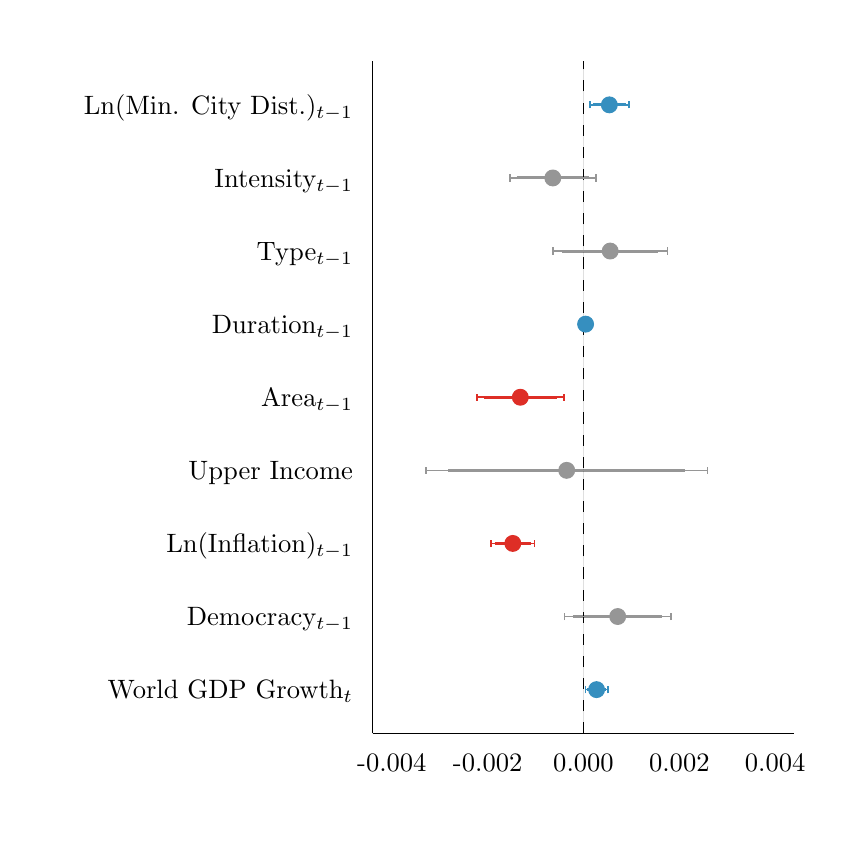
\begin{tikzpicture}[x=1pt,y=1pt]
\definecolor[named]{fillColor}{rgb}{1.00,1.00,1.00}
\path[use as bounding box,fill=fillColor,fill opacity=0.00] (0,0) rectangle (289.08,289.08);
\begin{scope}
\path[clip] (  0.00,  0.00) rectangle (289.08,289.08);
\definecolor[named]{drawColor}{rgb}{1.00,1.00,1.00}
\definecolor[named]{fillColor}{rgb}{1.00,1.00,1.00}

\path[draw=drawColor,line width= 0.6pt,line join=round,line cap=round,fill=fillColor] ( -0.00,  0.00) rectangle (289.08,289.08);
\end{scope}
\begin{scope}
\path[clip] (124.66, 34.03) rectangle (277.03,277.03);
\definecolor[named]{fillColor}{rgb}{1.00,1.00,1.00}

\path[fill=fillColor] (124.66, 34.03) rectangle (277.04,277.03);
\definecolor[named]{drawColor}{rgb}{0.21,0.56,0.75}
\definecolor[named]{fillColor}{rgb}{0.21,0.56,0.75}

\path[draw=drawColor,draw opacity=0.30,line width= 0.3pt,line join=round,fill=fillColor,fill opacity=0.30] (201.54, 49.88) -- (209.61, 49.88);
\definecolor[named]{drawColor}{rgb}{0.59,0.59,0.59}
\definecolor[named]{fillColor}{rgb}{0.59,0.59,0.59}

\path[draw=drawColor,draw opacity=0.30,line width= 0.3pt,line join=round,fill=fillColor,fill opacity=0.30] (193.96, 76.30) -- (232.45, 76.30);
\definecolor[named]{drawColor}{rgb}{0.87,0.18,0.15}
\definecolor[named]{fillColor}{rgb}{0.87,0.18,0.15}

\path[draw=drawColor,draw opacity=0.30,line width= 0.3pt,line join=round,fill=fillColor,fill opacity=0.30] (167.42,102.71) -- (183.20,102.71);
\definecolor[named]{drawColor}{rgb}{0.59,0.59,0.59}
\definecolor[named]{fillColor}{rgb}{0.59,0.59,0.59}

\path[draw=drawColor,draw opacity=0.30,line width= 0.3pt,line join=round,fill=fillColor,fill opacity=0.30] (143.88,129.12) -- (245.67,129.12);
\definecolor[named]{drawColor}{rgb}{0.87,0.18,0.15}
\definecolor[named]{fillColor}{rgb}{0.87,0.18,0.15}

\path[draw=drawColor,draw opacity=0.30,line width= 0.3pt,line join=round,fill=fillColor,fill opacity=0.30] (162.34,155.53) -- (193.68,155.53);
\definecolor[named]{drawColor}{rgb}{0.21,0.56,0.75}
\definecolor[named]{fillColor}{rgb}{0.21,0.56,0.75}

\path[draw=drawColor,draw opacity=0.30,line width= 0.3pt,line join=round,fill=fillColor,fill opacity=0.30] (200.93,181.95) -- (202.27,181.95);
\definecolor[named]{drawColor}{rgb}{0.59,0.59,0.59}
\definecolor[named]{fillColor}{rgb}{0.59,0.59,0.59}

\path[draw=drawColor,draw opacity=0.30,line width= 0.3pt,line join=round,fill=fillColor,fill opacity=0.30] (189.78,208.36) -- (231.19,208.36);

\path[draw=drawColor,draw opacity=0.30,line width= 0.3pt,line join=round,fill=fillColor,fill opacity=0.30] (174.23,234.77) -- (205.28,234.77);
\definecolor[named]{drawColor}{rgb}{0.21,0.56,0.75}
\definecolor[named]{fillColor}{rgb}{0.21,0.56,0.75}

\path[draw=drawColor,draw opacity=0.30,line width= 0.3pt,line join=round,fill=fillColor,fill opacity=0.30] (203.17,261.19) -- (217.19,261.19);
\definecolor[named]{drawColor}{rgb}{0.21,0.56,0.75}
\definecolor[named]{fillColor}{rgb}{0.21,0.56,0.75}

\path[draw=drawColor,line width= 1.1pt,line join=round,fill=fillColor] (202.19, 49.88) -- (208.96, 49.88);
\definecolor[named]{drawColor}{rgb}{0.59,0.59,0.59}
\definecolor[named]{fillColor}{rgb}{0.59,0.59,0.59}

\path[draw=drawColor,line width= 1.1pt,line join=round,fill=fillColor] (197.05, 76.30) -- (229.35, 76.30);
\definecolor[named]{drawColor}{rgb}{0.87,0.18,0.15}
\definecolor[named]{fillColor}{rgb}{0.87,0.18,0.15}

\path[draw=drawColor,line width= 1.1pt,line join=round,fill=fillColor] (168.69,102.71) -- (181.93,102.71);
\definecolor[named]{drawColor}{rgb}{0.59,0.59,0.59}
\definecolor[named]{fillColor}{rgb}{0.59,0.59,0.59}

\path[draw=drawColor,line width= 1.1pt,line join=round,fill=fillColor] (152.06,129.12) -- (237.49,129.12);
\definecolor[named]{drawColor}{rgb}{0.87,0.18,0.15}
\definecolor[named]{fillColor}{rgb}{0.87,0.18,0.15}

\path[draw=drawColor,line width= 1.1pt,line join=round,fill=fillColor] (164.86,155.53) -- (191.16,155.53);
\definecolor[named]{drawColor}{rgb}{0.21,0.56,0.75}
\definecolor[named]{fillColor}{rgb}{0.21,0.56,0.75}

\path[draw=drawColor,line width= 1.1pt,line join=round,fill=fillColor] (201.04,181.95) -- (202.16,181.95);
\definecolor[named]{drawColor}{rgb}{0.59,0.59,0.59}
\definecolor[named]{fillColor}{rgb}{0.59,0.59,0.59}

\path[draw=drawColor,line width= 1.1pt,line join=round,fill=fillColor] (193.11,208.36) -- (227.86,208.36);

\path[draw=drawColor,line width= 1.1pt,line join=round,fill=fillColor] (176.73,234.77) -- (202.79,234.77);
\definecolor[named]{drawColor}{rgb}{0.21,0.56,0.75}
\definecolor[named]{fillColor}{rgb}{0.21,0.56,0.75}

\path[draw=drawColor,line width= 1.1pt,line join=round,fill=fillColor] (204.30,261.19) -- (216.06,261.19);
\definecolor[named]{drawColor}{rgb}{0.00,0.00,0.00}
\definecolor[named]{fillColor}{rgb}{0.00,0.00,0.00}

\path[draw=drawColor,line width= 0.6pt,dash pattern=on 4pt off 4pt ,line join=round,fill=fillColor] (200.85, 34.03) -- (200.85,277.03);
\definecolor[named]{drawColor}{rgb}{0.21,0.56,0.75}
\definecolor[named]{fillColor}{rgb}{0.21,0.56,0.75}

\path[draw=drawColor,line width= 0.4pt,line join=round,line cap=round,fill=fillColor] (210.18,261.19) circle (  2.85);
\definecolor[named]{drawColor}{rgb}{0.59,0.59,0.59}
\definecolor[named]{fillColor}{rgb}{0.59,0.59,0.59}

\path[draw=drawColor,line width= 0.4pt,line join=round,line cap=round,fill=fillColor] (189.76,234.77) circle (  2.85);

\path[draw=drawColor,line width= 0.4pt,line join=round,line cap=round,fill=fillColor] (210.49,208.36) circle (  2.85);
\definecolor[named]{drawColor}{rgb}{0.21,0.56,0.75}
\definecolor[named]{fillColor}{rgb}{0.21,0.56,0.75}

\path[draw=drawColor,line width= 0.4pt,line join=round,line cap=round,fill=fillColor] (201.60,181.95) circle (  2.85);
\definecolor[named]{drawColor}{rgb}{0.87,0.18,0.15}
\definecolor[named]{fillColor}{rgb}{0.87,0.18,0.15}

\path[draw=drawColor,line width= 0.4pt,line join=round,line cap=round,fill=fillColor] (178.01,155.53) circle (  2.85);
\definecolor[named]{drawColor}{rgb}{0.59,0.59,0.59}
\definecolor[named]{fillColor}{rgb}{0.59,0.59,0.59}

\path[draw=drawColor,line width= 0.4pt,line join=round,line cap=round,fill=fillColor] (194.77,129.12) circle (  2.85);
\definecolor[named]{drawColor}{rgb}{0.87,0.18,0.15}
\definecolor[named]{fillColor}{rgb}{0.87,0.18,0.15}

\path[draw=drawColor,line width= 0.4pt,line join=round,line cap=round,fill=fillColor] (175.31,102.71) circle (  2.85);
\definecolor[named]{drawColor}{rgb}{0.59,0.59,0.59}
\definecolor[named]{fillColor}{rgb}{0.59,0.59,0.59}

\path[draw=drawColor,line width= 0.4pt,line join=round,line cap=round,fill=fillColor] (213.20, 76.30) circle (  2.85);
\definecolor[named]{drawColor}{rgb}{0.21,0.56,0.75}
\definecolor[named]{fillColor}{rgb}{0.21,0.56,0.75}

\path[draw=drawColor,line width= 0.4pt,line join=round,line cap=round,fill=fillColor] (205.57, 49.88) circle (  2.85);

\path[draw=drawColor,line width= 0.6pt,line join=round] (209.61, 48.56) --
	(209.61, 51.20);

\path[draw=drawColor,line width= 0.6pt,line join=round] (209.61, 49.88) --
	(201.54, 49.88);

\path[draw=drawColor,line width= 0.6pt,line join=round] (201.54, 48.56) --
	(201.54, 51.20);
\definecolor[named]{drawColor}{rgb}{0.59,0.59,0.59}

\path[draw=drawColor,line width= 0.6pt,line join=round] (232.45, 74.97) --
	(232.45, 77.62);

\path[draw=drawColor,line width= 0.6pt,line join=round] (232.45, 76.30) --
	(193.96, 76.30);

\path[draw=drawColor,line width= 0.6pt,line join=round] (193.96, 74.97) --
	(193.96, 77.62);
\definecolor[named]{drawColor}{rgb}{0.87,0.18,0.15}

\path[draw=drawColor,line width= 0.6pt,line join=round] (183.20,101.39) --
	(183.20,104.03);

\path[draw=drawColor,line width= 0.6pt,line join=round] (183.20,102.71) --
	(167.42,102.71);

\path[draw=drawColor,line width= 0.6pt,line join=round] (167.42,101.39) --
	(167.42,104.03);
\definecolor[named]{drawColor}{rgb}{0.59,0.59,0.59}

\path[draw=drawColor,line width= 0.6pt,line join=round] (245.67,127.80) --
	(245.67,130.44);

\path[draw=drawColor,line width= 0.6pt,line join=round] (245.67,129.12) --
	(143.88,129.12);

\path[draw=drawColor,line width= 0.6pt,line join=round] (143.88,127.80) --
	(143.88,130.44);
\definecolor[named]{drawColor}{rgb}{0.87,0.18,0.15}

\path[draw=drawColor,line width= 0.6pt,line join=round] (193.68,154.21) --
	(193.68,156.86);

\path[draw=drawColor,line width= 0.6pt,line join=round] (193.68,155.53) --
	(162.34,155.53);

\path[draw=drawColor,line width= 0.6pt,line join=round] (162.34,154.21) --
	(162.34,156.86);
\definecolor[named]{drawColor}{rgb}{0.21,0.56,0.75}

\path[draw=drawColor,line width= 0.6pt,line join=round] (202.27,180.63) --
	(202.27,183.27);

\path[draw=drawColor,line width= 0.6pt,line join=round] (202.27,181.95) --
	(200.93,181.95);

\path[draw=drawColor,line width= 0.6pt,line join=round] (200.93,180.63) --
	(200.93,183.27);
\definecolor[named]{drawColor}{rgb}{0.59,0.59,0.59}

\path[draw=drawColor,line width= 0.6pt,line join=round] (231.19,207.04) --
	(231.19,209.68);

\path[draw=drawColor,line width= 0.6pt,line join=round] (231.19,208.36) --
	(189.78,208.36);

\path[draw=drawColor,line width= 0.6pt,line join=round] (189.78,207.04) --
	(189.78,209.68);

\path[draw=drawColor,line width= 0.6pt,line join=round] (205.28,233.45) --
	(205.28,236.09);

\path[draw=drawColor,line width= 0.6pt,line join=round] (205.28,234.77) --
	(174.23,234.77);

\path[draw=drawColor,line width= 0.6pt,line join=round] (174.23,233.45) --
	(174.23,236.09);
\definecolor[named]{drawColor}{rgb}{0.21,0.56,0.75}

\path[draw=drawColor,line width= 0.6pt,line join=round] (217.19,259.87) --
	(217.19,262.51);

\path[draw=drawColor,line width= 0.6pt,line join=round] (217.19,261.19) --
	(203.17,261.19);

\path[draw=drawColor,line width= 0.6pt,line join=round] (203.17,259.87) --
	(203.17,262.51);
\end{scope}
\begin{scope}
\path[clip] (  0.00,  0.00) rectangle (289.08,289.08);
\definecolor[named]{drawColor}{rgb}{0.00,0.00,0.00}

\path[draw=drawColor,line width= 0.6pt,line join=round] (124.66, 34.03) --
	(124.66,277.03);
\end{scope}
\begin{scope}
\path[clip] (  0.00,  0.00) rectangle (289.08,289.08);
\definecolor[named]{drawColor}{rgb}{0.00,0.00,0.00}

\node[text=drawColor,anchor=base east,inner sep=0pt, outer sep=0pt, scale=  0.96] at (117.55, 46.58) {World GDP Growth$_{t}$};

\node[text=drawColor,anchor=base east,inner sep=0pt, outer sep=0pt, scale=  0.96] at (117.55, 72.99) {Democracy$_{t-1}$};

\node[text=drawColor,anchor=base east,inner sep=0pt, outer sep=0pt, scale=  0.96] at (117.55, 99.40) {Ln(Inflation)$_{t-1}$};

\node[text=drawColor,anchor=base east,inner sep=0pt, outer sep=0pt, scale=  0.96] at (117.55,125.82) {Upper Income};

\node[text=drawColor,anchor=base east,inner sep=0pt, outer sep=0pt, scale=  0.96] at (117.55,152.23) {Area$_{t-1}$};

\node[text=drawColor,anchor=base east,inner sep=0pt, outer sep=0pt, scale=  0.96] at (117.55,178.64) {Duration$_{t-1}$};

\node[text=drawColor,anchor=base east,inner sep=0pt, outer sep=0pt, scale=  0.96] at (117.55,205.06) {Type$_{t-1}$};

\node[text=drawColor,anchor=base east,inner sep=0pt, outer sep=0pt, scale=  0.96] at (117.55,231.47) {Intensity$_{t-1}$};

\node[text=drawColor,anchor=base east,inner sep=0pt, outer sep=0pt, scale=  0.96] at (117.55,257.88) {Ln(Min. City Dist.)$_{t-1}$};
\end{scope}
\begin{scope}
\path[clip] (  0.00,  0.00) rectangle (289.08,289.08);
\definecolor[named]{drawColor}{rgb}{0.00,0.00,0.00}

\path[draw=drawColor,line width= 0.6pt,line join=round] (124.66, 34.03) --
	(277.03, 34.03);
\end{scope}
\begin{scope}
\path[clip] (  0.00,  0.00) rectangle (289.08,289.08);
\definecolor[named]{drawColor}{rgb}{0.00,0.00,0.00}

\node[text=drawColor,anchor=base,inner sep=0pt, outer sep=0pt, scale=  0.96] at (131.59, 20.31) {-0.004};

\node[text=drawColor,anchor=base,inner sep=0pt, outer sep=0pt, scale=  0.96] at (166.22, 20.31) {-0.002};

\node[text=drawColor,anchor=base,inner sep=0pt, outer sep=0pt, scale=  0.96] at (200.85, 20.31) {0.000};

\node[text=drawColor,anchor=base,inner sep=0pt, outer sep=0pt, scale=  0.96] at (235.48, 20.31) {0.002};

\node[text=drawColor,anchor=base,inner sep=0pt, outer sep=0pt, scale=  0.96] at (270.11, 20.31) {0.004};
\end{scope}
\end{tikzpicture}
}
		\label{fig:cityCoef}}
	\end{tabular}
	\caption{Regression results using conflict distance from capital city on the left, and the chart on the right shows regression results using minimum conflict distance from any major city. Darker colors indicates that the coefficient estimate is significantly different from zero at a 95\% CI, while lighter the same for a 90\% CI. Grey indicates that the estimate is not significantly different from zero at either of those intervals.}
	\label{fig:coefplot}
\end{figure}

To ensure that our parameter estimates are robust to changes in our sample, we run a six-fold cross-validation. This analysis helps us to understand whether some of the subsets in our dataset follow a different pattern than what is in the broader set \citep{beck2008time}. To conduct the cross-validation, we randomly split the 68 country observations in our dataset into seven approximately equal subsets. Each subset ends up containing a minimum of approximately 65 cases. We then run each model shown in figure \ref{fig:coefplot} seven times, where in each iteration we left out one subsample. The results of this analysis are depicted in \ref{fig:crossPlot}, and we can clearly see that the parameter estimates for our two spatial proximity variables remain consistent across the exclusion of any of the folds.

\begin{figure}
	\centering
	\resizebox{.8\textwidth}{!}{% Created by tikzDevice version 0.7.0 on 2014-10-06 19:49:11
% !TEX encoding = UTF-8 Unicode
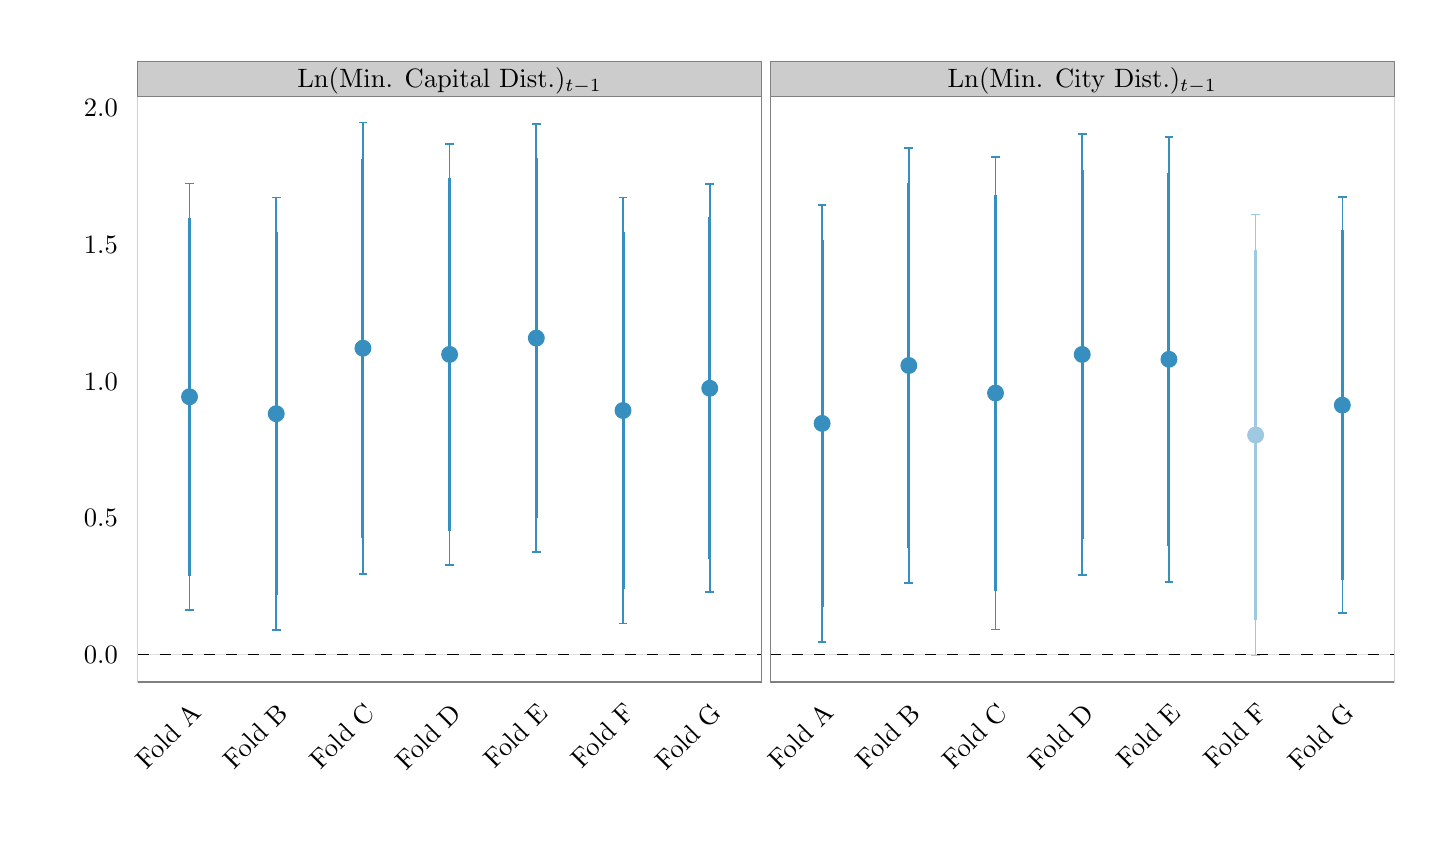
\begin{tikzpicture}[x=1pt,y=1pt]
\definecolor[named]{fillColor}{rgb}{1.00,1.00,1.00}
\path[use as bounding box,fill=fillColor,fill opacity=0.00] (0,0) rectangle (505.89,289.08);
\begin{scope}
\path[clip] (  0.00,  0.00) rectangle (505.89,289.08);
\definecolor[named]{drawColor}{rgb}{1.00,1.00,1.00}
\definecolor[named]{fillColor}{rgb}{1.00,1.00,1.00}

\path[draw=drawColor,line width= 0.6pt,line join=round,line cap=round,fill=fillColor] (  0.00,  0.00) rectangle (505.89,289.08);
\end{scope}
\begin{scope}
\path[clip] ( 39.69, 52.60) rectangle (265.26,264.40);
\definecolor[named]{fillColor}{rgb}{1.00,1.00,1.00}

\path[fill=fillColor] ( 39.69, 52.60) rectangle (265.26,264.40);
\definecolor[named]{drawColor}{rgb}{0.21,0.56,0.75}
\definecolor[named]{fillColor}{rgb}{0.21,0.56,0.75}

\path[draw=drawColor,draw opacity=0.30,line width= 0.3pt,line join=round,fill=fillColor,fill opacity=0.30] ( 58.48, 78.70) -- ( 58.48,232.72);

\path[draw=drawColor,draw opacity=0.30,line width= 0.3pt,line join=round,fill=fillColor,fill opacity=0.30] ( 89.81, 71.45) -- ( 89.81,227.72);

\path[draw=drawColor,draw opacity=0.30,line width= 0.3pt,line join=round,fill=fillColor,fill opacity=0.30] (121.14, 91.74) -- (121.14,254.77);

\path[draw=drawColor,draw opacity=0.30,line width= 0.3pt,line join=round,fill=fillColor,fill opacity=0.30] (152.47, 95.01) -- (152.47,247.01);

\path[draw=drawColor,draw opacity=0.30,line width= 0.3pt,line join=round,fill=fillColor,fill opacity=0.30] (183.80, 99.56) -- (183.80,254.25);

\path[draw=drawColor,draw opacity=0.30,line width= 0.3pt,line join=round,fill=fillColor,fill opacity=0.30] (215.13, 73.72) -- (215.13,227.75);

\path[draw=drawColor,draw opacity=0.30,line width= 0.3pt,line join=round,fill=fillColor,fill opacity=0.30] (246.46, 85.07) -- (246.46,232.49);
\definecolor[named]{drawColor}{rgb}{0.21,0.56,0.75}
\definecolor[named]{fillColor}{rgb}{0.21,0.56,0.75}

\path[draw=drawColor,line width= 1.1pt,line join=round,fill=fillColor] ( 58.48, 91.09) -- ( 58.48,220.34);

\path[draw=drawColor,line width= 1.1pt,line join=round,fill=fillColor] ( 89.81, 84.01) -- ( 89.81,215.15);

\path[draw=drawColor,line width= 1.1pt,line join=round,fill=fillColor] (121.14,104.85) -- (121.14,241.67);

\path[draw=drawColor,line width= 1.1pt,line join=round,fill=fillColor] (152.47,107.23) -- (152.47,234.79);

\path[draw=drawColor,line width= 1.1pt,line join=round,fill=fillColor] (183.80,111.99) -- (183.80,241.82);

\path[draw=drawColor,line width= 1.1pt,line join=round,fill=fillColor] (215.13, 86.11) -- (215.13,215.37);

\path[draw=drawColor,line width= 1.1pt,line join=round,fill=fillColor] (246.46, 96.92) -- (246.46,220.64);
\definecolor[named]{drawColor}{rgb}{0.00,0.00,0.00}
\definecolor[named]{fillColor}{rgb}{0.00,0.00,0.00}

\path[draw=drawColor,line width= 0.6pt,dash pattern=on 4pt off 4pt ,line join=round,fill=fillColor] ( 39.69, 62.52) -- (265.26, 62.52);
\definecolor[named]{drawColor}{rgb}{0.21,0.56,0.75}
\definecolor[named]{fillColor}{rgb}{0.21,0.56,0.75}

\path[draw=drawColor,line width= 0.4pt,line join=round,line cap=round,fill=fillColor] ( 58.48,155.71) circle (  2.85);

\path[draw=drawColor,line width= 0.4pt,line join=round,line cap=round,fill=fillColor] ( 89.81,149.58) circle (  2.85);

\path[draw=drawColor,line width= 0.4pt,line join=round,line cap=round,fill=fillColor] (121.14,173.26) circle (  2.85);

\path[draw=drawColor,line width= 0.4pt,line join=round,line cap=round,fill=fillColor] (152.47,171.01) circle (  2.85);

\path[draw=drawColor,line width= 0.4pt,line join=round,line cap=round,fill=fillColor] (183.80,176.91) circle (  2.85);

\path[draw=drawColor,line width= 0.4pt,line join=round,line cap=round,fill=fillColor] (215.13,150.74) circle (  2.85);

\path[draw=drawColor,line width= 0.4pt,line join=round,line cap=round,fill=fillColor] (246.46,158.78) circle (  2.85);

\path[draw=drawColor,line width= 0.6pt,line join=round] ( 56.92,232.72) --
	( 60.05,232.72);

\path[draw=drawColor,line width= 0.6pt,line join=round] ( 58.48,232.72) --
	( 58.48, 78.70);

\path[draw=drawColor,line width= 0.6pt,line join=round] ( 56.92, 78.70) --
	( 60.05, 78.70);

\path[draw=drawColor,line width= 0.6pt,line join=round] ( 88.25,227.72) --
	( 91.38,227.72);

\path[draw=drawColor,line width= 0.6pt,line join=round] ( 89.81,227.72) --
	( 89.81, 71.45);

\path[draw=drawColor,line width= 0.6pt,line join=round] ( 88.25, 71.45) --
	( 91.38, 71.45);

\path[draw=drawColor,line width= 0.6pt,line join=round] (119.58,254.77) --
	(122.71,254.77);

\path[draw=drawColor,line width= 0.6pt,line join=round] (121.14,254.77) --
	(121.14, 91.74);

\path[draw=drawColor,line width= 0.6pt,line join=round] (119.58, 91.74) --
	(122.71, 91.74);

\path[draw=drawColor,line width= 0.6pt,line join=round] (150.91,247.01) --
	(154.04,247.01);

\path[draw=drawColor,line width= 0.6pt,line join=round] (152.47,247.01) --
	(152.47, 95.01);

\path[draw=drawColor,line width= 0.6pt,line join=round] (150.91, 95.01) --
	(154.04, 95.01);

\path[draw=drawColor,line width= 0.6pt,line join=round] (182.24,254.25) --
	(185.37,254.25);

\path[draw=drawColor,line width= 0.6pt,line join=round] (183.80,254.25) --
	(183.80, 99.56);

\path[draw=drawColor,line width= 0.6pt,line join=round] (182.24, 99.56) --
	(185.37, 99.56);

\path[draw=drawColor,line width= 0.6pt,line join=round] (213.57,227.75) --
	(216.70,227.75);

\path[draw=drawColor,line width= 0.6pt,line join=round] (215.13,227.75) --
	(215.13, 73.72);

\path[draw=drawColor,line width= 0.6pt,line join=round] (213.57, 73.72) --
	(216.70, 73.72);

\path[draw=drawColor,line width= 0.6pt,line join=round] (244.90,232.49) --
	(248.03,232.49);

\path[draw=drawColor,line width= 0.6pt,line join=round] (246.46,232.49) --
	(246.46, 85.07);

\path[draw=drawColor,line width= 0.6pt,line join=round] (244.90, 85.07) --
	(248.03, 85.07);
\definecolor[named]{drawColor}{rgb}{0.50,0.50,0.50}

\path[draw=drawColor,line width= 0.6pt,line join=round,line cap=round] ( 39.69, 52.60) rectangle (265.26,264.40);
\end{scope}
\begin{scope}
\path[clip] (268.27, 52.60) rectangle (493.85,264.40);
\definecolor[named]{fillColor}{rgb}{1.00,1.00,1.00}

\path[fill=fillColor] (268.27, 52.60) rectangle (493.85,264.40);
\definecolor[named]{drawColor}{rgb}{0.21,0.56,0.75}
\definecolor[named]{fillColor}{rgb}{0.21,0.56,0.75}

\path[draw=drawColor,draw opacity=0.30,line width= 0.3pt,line join=round,fill=fillColor,fill opacity=0.30] (287.07, 67.19) -- (287.07,224.97);

\path[draw=drawColor,draw opacity=0.30,line width= 0.3pt,line join=round,fill=fillColor,fill opacity=0.30] (318.40, 88.38) -- (318.40,245.63);

\path[draw=drawColor,draw opacity=0.30,line width= 0.3pt,line join=round,fill=fillColor,fill opacity=0.30] (349.73, 71.61) -- (349.73,242.46);

\path[draw=drawColor,draw opacity=0.30,line width= 0.3pt,line join=round,fill=fillColor,fill opacity=0.30] (381.06, 91.40) -- (381.06,250.60);

\path[draw=drawColor,draw opacity=0.30,line width= 0.3pt,line join=round,fill=fillColor,fill opacity=0.30] (412.39, 88.88) -- (412.39,249.59);
\definecolor[named]{drawColor}{rgb}{0.62,0.79,0.88}
\definecolor[named]{fillColor}{rgb}{0.62,0.79,0.88}

\path[draw=drawColor,draw opacity=0.30,line width= 0.3pt,line join=round,fill=fillColor,fill opacity=0.30] (443.72, 62.23) -- (443.72,221.53);
\definecolor[named]{drawColor}{rgb}{0.21,0.56,0.75}
\definecolor[named]{fillColor}{rgb}{0.21,0.56,0.75}

\path[draw=drawColor,draw opacity=0.30,line width= 0.3pt,line join=round,fill=fillColor,fill opacity=0.30] (475.05, 77.47) -- (475.05,227.88);
\definecolor[named]{drawColor}{rgb}{0.21,0.56,0.75}
\definecolor[named]{fillColor}{rgb}{0.21,0.56,0.75}

\path[draw=drawColor,line width= 1.1pt,line join=round,fill=fillColor] (287.07, 79.88) -- (287.07,212.29);

\path[draw=drawColor,line width= 1.1pt,line join=round,fill=fillColor] (318.40,101.02) -- (318.40,232.99);

\path[draw=drawColor,line width= 1.1pt,line join=round,fill=fillColor] (349.73, 85.35) -- (349.73,228.72);

\path[draw=drawColor,line width= 1.1pt,line join=round,fill=fillColor] (381.06,104.20) -- (381.06,237.81);

\path[draw=drawColor,line width= 1.1pt,line join=round,fill=fillColor] (412.39,101.80) -- (412.39,236.67);
\definecolor[named]{drawColor}{rgb}{0.62,0.79,0.88}
\definecolor[named]{fillColor}{rgb}{0.62,0.79,0.88}

\path[draw=drawColor,line width= 1.1pt,line join=round,fill=fillColor] (443.72, 75.03) -- (443.72,208.73);
\definecolor[named]{drawColor}{rgb}{0.21,0.56,0.75}
\definecolor[named]{fillColor}{rgb}{0.21,0.56,0.75}

\path[draw=drawColor,line width= 1.1pt,line join=round,fill=fillColor] (475.05, 89.56) -- (475.05,215.79);
\definecolor[named]{drawColor}{rgb}{0.00,0.00,0.00}
\definecolor[named]{fillColor}{rgb}{0.00,0.00,0.00}

\path[draw=drawColor,line width= 0.6pt,dash pattern=on 4pt off 4pt ,line join=round,fill=fillColor] (268.27, 62.52) -- (493.85, 62.52);
\definecolor[named]{drawColor}{rgb}{0.21,0.56,0.75}
\definecolor[named]{fillColor}{rgb}{0.21,0.56,0.75}

\path[draw=drawColor,line width= 0.4pt,line join=round,line cap=round,fill=fillColor] (287.07,146.08) circle (  2.85);

\path[draw=drawColor,line width= 0.4pt,line join=round,line cap=round,fill=fillColor] (318.40,167.00) circle (  2.85);

\path[draw=drawColor,line width= 0.4pt,line join=round,line cap=round,fill=fillColor] (349.73,157.04) circle (  2.85);

\path[draw=drawColor,line width= 0.4pt,line join=round,line cap=round,fill=fillColor] (381.06,171.00) circle (  2.85);

\path[draw=drawColor,line width= 0.4pt,line join=round,line cap=round,fill=fillColor] (412.39,169.24) circle (  2.85);
\definecolor[named]{drawColor}{rgb}{0.62,0.79,0.88}
\definecolor[named]{fillColor}{rgb}{0.62,0.79,0.88}

\path[draw=drawColor,line width= 0.4pt,line join=round,line cap=round,fill=fillColor] (443.72,141.88) circle (  2.85);
\definecolor[named]{drawColor}{rgb}{0.21,0.56,0.75}
\definecolor[named]{fillColor}{rgb}{0.21,0.56,0.75}

\path[draw=drawColor,line width= 0.4pt,line join=round,line cap=round,fill=fillColor] (475.05,152.67) circle (  2.85);

\path[draw=drawColor,line width= 0.6pt,line join=round] (285.50,224.97) --
	(288.64,224.97);

\path[draw=drawColor,line width= 0.6pt,line join=round] (287.07,224.97) --
	(287.07, 67.19);

\path[draw=drawColor,line width= 0.6pt,line join=round] (285.50, 67.19) --
	(288.64, 67.19);

\path[draw=drawColor,line width= 0.6pt,line join=round] (316.83,245.63) --
	(319.97,245.63);

\path[draw=drawColor,line width= 0.6pt,line join=round] (318.40,245.63) --
	(318.40, 88.38);

\path[draw=drawColor,line width= 0.6pt,line join=round] (316.83, 88.38) --
	(319.97, 88.38);

\path[draw=drawColor,line width= 0.6pt,line join=round] (348.16,242.46) --
	(351.30,242.46);

\path[draw=drawColor,line width= 0.6pt,line join=round] (349.73,242.46) --
	(349.73, 71.61);

\path[draw=drawColor,line width= 0.6pt,line join=round] (348.16, 71.61) --
	(351.30, 71.61);

\path[draw=drawColor,line width= 0.6pt,line join=round] (379.49,250.60) --
	(382.62,250.60);

\path[draw=drawColor,line width= 0.6pt,line join=round] (381.06,250.60) --
	(381.06, 91.40);

\path[draw=drawColor,line width= 0.6pt,line join=round] (379.49, 91.40) --
	(382.62, 91.40);

\path[draw=drawColor,line width= 0.6pt,line join=round] (410.82,249.59) --
	(413.95,249.59);

\path[draw=drawColor,line width= 0.6pt,line join=round] (412.39,249.59) --
	(412.39, 88.88);

\path[draw=drawColor,line width= 0.6pt,line join=round] (410.82, 88.88) --
	(413.95, 88.88);
\definecolor[named]{drawColor}{rgb}{0.62,0.79,0.88}

\path[draw=drawColor,line width= 0.6pt,line join=round] (442.15,221.53) --
	(445.28,221.53);

\path[draw=drawColor,line width= 0.6pt,line join=round] (443.72,221.53) --
	(443.72, 62.23);

\path[draw=drawColor,line width= 0.6pt,line join=round] (442.15, 62.23) --
	(445.28, 62.23);
\definecolor[named]{drawColor}{rgb}{0.21,0.56,0.75}

\path[draw=drawColor,line width= 0.6pt,line join=round] (473.48,227.88) --
	(476.61,227.88);

\path[draw=drawColor,line width= 0.6pt,line join=round] (475.05,227.88) --
	(475.05, 77.47);

\path[draw=drawColor,line width= 0.6pt,line join=round] (473.48, 77.47) --
	(476.61, 77.47);
\definecolor[named]{drawColor}{rgb}{0.50,0.50,0.50}

\path[draw=drawColor,line width= 0.6pt,line join=round,line cap=round] (268.27, 52.60) rectangle (493.85,264.40);
\end{scope}
\begin{scope}
\path[clip] (  0.00,  0.00) rectangle (505.89,289.08);
\definecolor[named]{drawColor}{rgb}{0.50,0.50,0.50}
\definecolor[named]{fillColor}{rgb}{0.80,0.80,0.80}

\path[draw=drawColor,line width= 0.2pt,line join=round,line cap=round,fill=fillColor] ( 39.69,264.40) rectangle (265.26,277.04);
\definecolor[named]{drawColor}{rgb}{0.00,0.00,0.00}

\node[text=drawColor,anchor=base,inner sep=0pt, outer sep=0pt, scale=  0.96] at (152.47,267.41) {Ln(Min. Capital Dist.)$_{t-1}$};
\end{scope}
\begin{scope}
\path[clip] (  0.00,  0.00) rectangle (505.89,289.08);
\definecolor[named]{drawColor}{rgb}{0.50,0.50,0.50}
\definecolor[named]{fillColor}{rgb}{0.80,0.80,0.80}

\path[draw=drawColor,line width= 0.2pt,line join=round,line cap=round,fill=fillColor] (268.27,264.40) rectangle (493.85,277.04);
\definecolor[named]{drawColor}{rgb}{0.00,0.00,0.00}

\node[text=drawColor,anchor=base,inner sep=0pt, outer sep=0pt, scale=  0.96] at (381.06,267.41) {Ln(Min. City Dist.)$_{t-1}$};
\end{scope}
\begin{scope}
\path[clip] (  0.00,  0.00) rectangle (505.89,289.08);
\definecolor[named]{drawColor}{rgb}{0.00,0.00,0.00}

\node[text=drawColor,anchor=base east,inner sep=0pt, outer sep=0pt, scale=  0.96] at ( 32.57, 59.21) {0.0};

\node[text=drawColor,anchor=base east,inner sep=0pt, outer sep=0pt, scale=  0.96] at ( 32.57,108.66) {0.5};

\node[text=drawColor,anchor=base east,inner sep=0pt, outer sep=0pt, scale=  0.96] at ( 32.57,158.12) {1.0};

\node[text=drawColor,anchor=base east,inner sep=0pt, outer sep=0pt, scale=  0.96] at ( 32.57,207.57) {1.5};

\node[text=drawColor,anchor=base east,inner sep=0pt, outer sep=0pt, scale=  0.96] at ( 32.57,257.02) {2.0};
\end{scope}
\begin{scope}
\path[clip] (  0.00,  0.00) rectangle (505.89,289.08);
\definecolor[named]{drawColor}{rgb}{0.00,0.00,0.00}

\node[text=drawColor,rotate= 45.00,anchor=base east,inner sep=0pt, outer sep=0pt, scale=  0.96] at ( 63.16, 40.81) {Fold A};

\node[text=drawColor,rotate= 45.00,anchor=base east,inner sep=0pt, outer sep=0pt, scale=  0.96] at ( 94.49, 40.81) {Fold B};

\node[text=drawColor,rotate= 45.00,anchor=base east,inner sep=0pt, outer sep=0pt, scale=  0.96] at (125.82, 40.81) {Fold C};

\node[text=drawColor,rotate= 45.00,anchor=base east,inner sep=0pt, outer sep=0pt, scale=  0.96] at (157.15, 40.81) {Fold D};

\node[text=drawColor,rotate= 45.00,anchor=base east,inner sep=0pt, outer sep=0pt, scale=  0.96] at (188.48, 40.81) {Fold E};

\node[text=drawColor,rotate= 45.00,anchor=base east,inner sep=0pt, outer sep=0pt, scale=  0.96] at (219.81, 40.81) {Fold F};

\node[text=drawColor,rotate= 45.00,anchor=base east,inner sep=0pt, outer sep=0pt, scale=  0.96] at (251.14, 40.81) {Fold G};
\end{scope}
\begin{scope}
\path[clip] (  0.00,  0.00) rectangle (505.89,289.08);
\definecolor[named]{drawColor}{rgb}{0.00,0.00,0.00}

\node[text=drawColor,rotate= 45.00,anchor=base east,inner sep=0pt, outer sep=0pt, scale=  0.96] at (291.74, 40.81) {Fold A};

\node[text=drawColor,rotate= 45.00,anchor=base east,inner sep=0pt, outer sep=0pt, scale=  0.96] at (323.07, 40.81) {Fold B};

\node[text=drawColor,rotate= 45.00,anchor=base east,inner sep=0pt, outer sep=0pt, scale=  0.96] at (354.40, 40.81) {Fold C};

\node[text=drawColor,rotate= 45.00,anchor=base east,inner sep=0pt, outer sep=0pt, scale=  0.96] at (385.73, 40.81) {Fold D};

\node[text=drawColor,rotate= 45.00,anchor=base east,inner sep=0pt, outer sep=0pt, scale=  0.96] at (417.06, 40.81) {Fold E};

\node[text=drawColor,rotate= 45.00,anchor=base east,inner sep=0pt, outer sep=0pt, scale=  0.96] at (448.39, 40.81) {Fold F};

\node[text=drawColor,rotate= 45.00,anchor=base east,inner sep=0pt, outer sep=0pt, scale=  0.96] at (479.72, 40.81) {Fold G};
\end{scope}
\end{tikzpicture}
}
	\caption{Each line here in the left panel shows the coefficient estimate of $Ln(Min. \; Capital \; Dist.)_{i,t-1}$ from rerunning the model on six random subsamples within the dataset. The panel on the right shows the same for $Ln(Min. \; City \; Dist.)_{i,t-1}$. All the covariates used in the initial model shown in figure \ref{fig:coefplot} were included as well.}
	\label{fig:crossPlot}
\end{figure}

To assess the substantive effect of these results, we conduct a number of simulations. We set up scenarios where we hold all variables to their median except for logged, minimum conflict distance, which we range from its minimum to maximum value. Next, we conduct 1,000 random draws from a multivariate normal to obtain distributions for the point estimates of each of the regression coefficients. After obtaining these distributions, we calculate the predicted value of GDP growth based on the conditions set by the scenarios. We plot the results of this analysis in figures \ref{fig:capSim} and \ref{fig:citySim}.  

\begin{figure}
	\centering
	\begin{tabular}{cc}
		\subfloat[SubFigure 1][Capital City]{
			\resizebox{.7\textwidth}{!}{% Created by tikzDevice version 0.7.0 on 2014-10-06 19:44:45
% !TEX encoding = UTF-8 Unicode
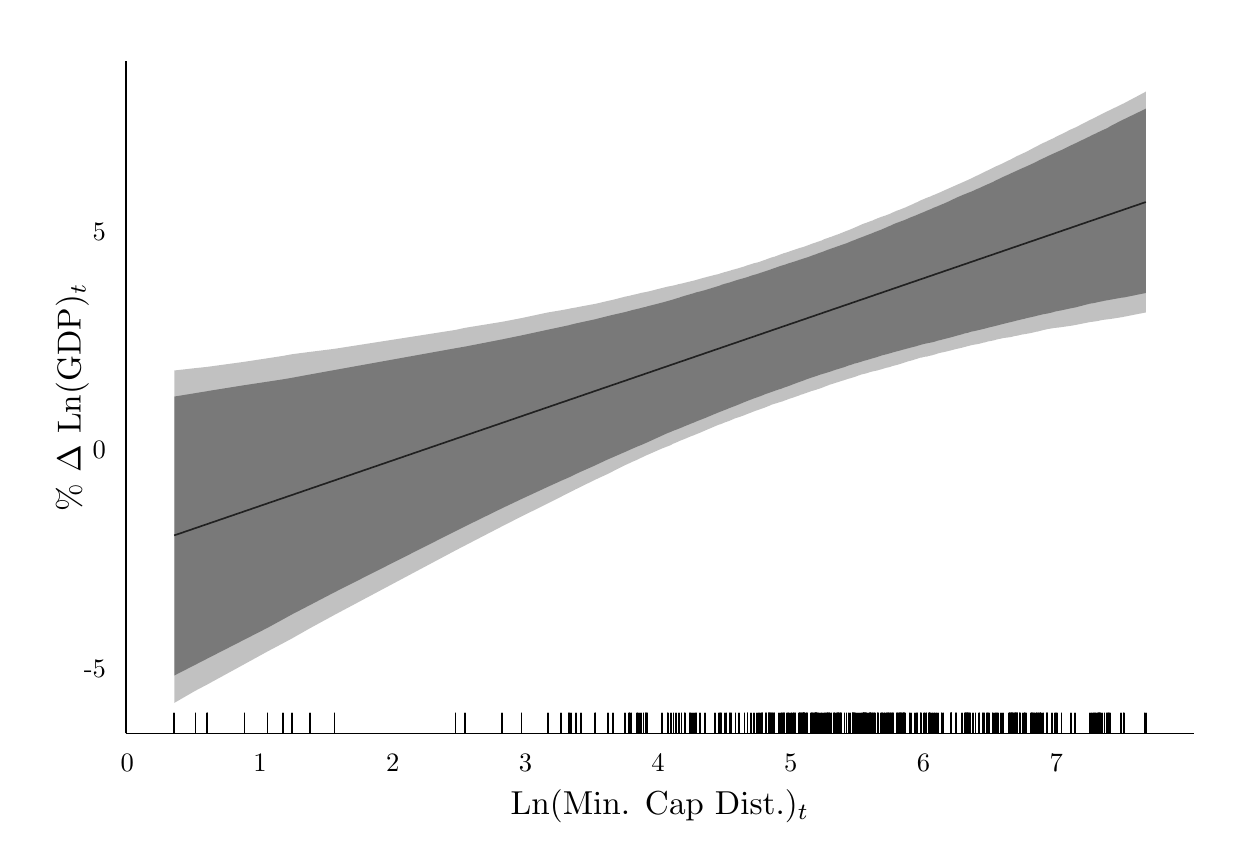
\begin{tikzpicture}[x=1pt,y=1pt]
\definecolor[named]{fillColor}{rgb}{1.00,1.00,1.00}
\path[use as bounding box,fill=fillColor,fill opacity=0.00] (0,0) rectangle (433.62,289.08);
\begin{scope}
\path[clip] (  0.00,  0.00) rectangle (433.62,289.08);
\definecolor[named]{drawColor}{rgb}{1.00,1.00,1.00}
\definecolor[named]{fillColor}{rgb}{1.00,1.00,1.00}

\path[draw=drawColor,line width= 0.6pt,line join=round,line cap=round,fill=fillColor] (  0.00,  0.00) rectangle (433.62,289.08);
\end{scope}
\begin{scope}
\path[clip] ( 35.42, 34.03) rectangle (421.57,277.03);
\definecolor[named]{fillColor}{rgb}{1.00,1.00,1.00}

\path[fill=fillColor] ( 35.42, 34.03) rectangle (421.57,277.03);
\definecolor[named]{drawColor}{rgb}{0.00,0.00,0.00}

\path[draw=drawColor,line width= 0.6pt,line join=round] ( 52.97,105.62) --
	( 60.61,108.24) --
	( 64.85,109.70) --
	( 64.98,109.74) --
	( 78.30,114.31) --
	( 86.71,117.20) --
	( 92.34,119.13) --
	( 95.59,120.24) --
	(101.92,122.42) --
	(110.88,125.49) --
	(154.64,140.51) --
	(158.01,141.66) --
	(171.43,146.26) --
	(178.49,148.69) --
	(187.92,151.92) --
	(192.71,153.57) --
	(195.62,154.56) --
	(195.71,154.59) --
	(196.35,154.81) --
	(198.04,155.39) --
	(199.87,156.02) --
	(204.99,157.78) --
	(205.19,157.85) --
	(209.65,159.38) --
	(211.50,160.01) --
	(215.87,161.51) --
	(217.33,162.01) --
	(217.43,162.05) --
	(217.68,162.13) --
	(218.17,162.30) --
	(220.17,162.99) --
	(220.33,163.04) --
	(220.93,163.25) --
	(221.63,163.49) --
	(222.58,163.81) --
	(223.29,164.06) --
	(223.54,164.14) --
	(223.59,164.16) --
	(224.00,164.30) --
	(229.14,166.07) --
	(231.15,166.76) --
	(231.34,166.82) --
	(232.39,167.18) --
	(233.34,167.51) --
	(234.25,167.82) --
	(235.24,168.16) --
	(236.22,168.49) --
	(237.40,168.90) --
	(237.41,168.90) --
	(239.29,169.55) --
	(239.31,169.55) --
	(240.03,169.80) --
	(240.80,170.06) --
	(241.27,170.23) --
	(241.65,170.36) --
	(242.95,170.80) --
	(244.78,171.43) --
	(248.30,172.64) --
	(249.74,173.13) --
	(250.22,173.30) --
	(250.38,173.35) --
	(250.69,173.46) --
	(251.97,173.90) --
	(252.46,174.07) --
	(253.69,174.49) --
	(253.89,174.55) --
	(254.34,174.71) --
	(255.74,175.19) --
	(256.94,175.60) --
	(258.99,176.31) --
	(260.08,176.68) --
	(260.16,176.71) --
	(261.39,177.13) --
	(262.57,177.53) --
	(263.47,177.84) --
	(264.14,178.07) --
	(264.43,178.17) --
	(264.94,178.35) --
	(265.11,178.40) --
	(265.48,178.53) --
	(265.54,178.55) --
	(266.69,178.95) --
	(266.70,178.95) --
	(267.74,179.31) --
	(267.83,179.34) --
	(267.95,179.38) --
	(268.15,179.45) --
	(268.32,179.51) --
	(268.51,179.57) --
	(268.75,179.66) --
	(269.12,179.78) --
	(269.30,179.84) --
	(269.75,180.00) --
	(269.91,180.05) --
	(271.51,180.60) --
	(272.31,180.88) --
	(272.40,180.91) --
	(272.91,181.08) --
	(273.01,181.11) --
	(273.29,181.21) --
	(273.48,181.28) --
	(274.31,181.56) --
	(274.85,181.75) --
	(274.88,181.76) --
	(275.50,181.97) --
	(276.03,182.15) --
	(276.14,182.19) --
	(276.73,182.39) --
	(276.77,182.41) --
	(277.28,182.58) --
	(277.37,182.61) --
	(278.83,183.11) --
	(278.93,183.15) --
	(278.99,183.17) --
	(279.03,183.18) --
	(279.36,183.30) --
	(279.83,183.46) --
	(279.90,183.48) --
	(280.21,183.59) --
	(280.36,183.64) --
	(280.41,183.66) --
	(280.47,183.68) --
	(280.50,183.68) --
	(280.60,183.72) --
	(280.63,183.73) --
	(281.16,183.91) --
	(281.52,184.03) --
	(281.60,184.06) --
	(283.10,184.58) --
	(283.28,184.64) --
	(283.34,184.66) --
	(283.74,184.80) --
	(283.80,184.82) --
	(284.26,184.97) --
	(284.43,185.03) --
	(284.75,185.14) --
	(284.80,185.16) --
	(284.81,185.16) --
	(284.81,185.16) --
	(284.84,185.18) --
	(284.88,185.19) --
	(285.44,185.38) --
	(285.67,185.46) --
	(286.04,185.59) --
	(286.70,185.81) --
	(286.95,185.90) --
	(287.76,186.18) --
	(288.16,186.31) --
	(288.45,186.41) --
	(288.86,186.55) --
	(289.03,186.61) --
	(289.13,186.65) --
	(289.30,186.70) --
	(289.61,186.81) --
	(289.71,186.85) --
	(289.99,186.94) --
	(290.44,187.10) --
	(291.29,187.39) --
	(291.45,187.44) --
	(291.58,187.49) --
	(292.20,187.70) --
	(292.36,187.75) --
	(292.77,187.89) --
	(292.78,187.90) --
	(292.85,187.92) --
	(292.94,187.95) --
	(293.49,188.14) --
	(293.61,188.18) --
	(293.90,188.28) --
	(293.94,188.30) --
	(295.12,188.70) --
	(295.85,188.95) --
	(296.61,189.21) --
	(297.11,189.38) --
	(297.99,189.68) --
	(298.09,189.72) --
	(298.13,189.74) --
	(298.21,189.76) --
	(298.45,189.84) --
	(298.48,189.85) --
	(298.71,189.93) --
	(298.89,190.00) --
	(299.22,190.11) --
	(300.07,190.40) --
	(300.69,190.61) --
	(301.34,190.83) --
	(301.81,191.00) --
	(301.86,191.01) --
	(302.06,191.08) --
	(302.08,191.09) --
	(302.20,191.13) --
	(302.30,191.16) --
	(302.45,191.22) --
	(302.52,191.24) --
	(302.61,191.27) --
	(302.89,191.37) --
	(302.93,191.38) --
	(303.17,191.46) --
	(304.10,191.78) --
	(304.31,191.85) --
	(304.47,191.91) --
	(304.48,191.91) --
	(304.60,191.95) --
	(304.68,191.98) --
	(305.11,192.13) --
	(305.28,192.19) --
	(305.76,192.35) --
	(305.86,192.39) --
	(306.15,192.49) --
	(307.03,192.79) --
	(307.16,192.83) --
	(307.37,192.90) --
	(308.42,193.27) --
	(308.63,193.34) --
	(308.79,193.39) --
	(309.08,193.49) --
	(309.55,193.65) --
	(309.72,193.71) --
	(310.36,193.93) --
	(310.45,193.96) --
	(310.80,194.08) --
	(310.98,194.14) --
	(311.09,194.18) --
	(311.49,194.32) --
	(311.71,194.39) --
	(311.87,194.45) --
	(312.39,194.63) --
	(312.68,194.73) --
	(312.75,194.75) --
	(314.09,195.21) --
	(314.12,195.22) --
	(314.55,195.37) --
	(314.84,195.47) --
	(315.05,195.54) --
	(315.28,195.62) --
	(315.54,195.71) --
	(315.61,195.73) --
	(315.65,195.75) --
	(316.29,195.97) --
	(316.37,195.99) --
	(316.58,196.06) --
	(316.61,196.07) --
	(316.72,196.11) --
	(317.13,196.25) --
	(318.60,196.76) --
	(319.14,196.94) --
	(320.71,197.48) --
	(321.34,197.70) --
	(321.47,197.74) --
	(322.56,198.12) --
	(322.64,198.14) --
	(322.93,198.24) --
	(323.98,198.60) --
	(324.06,198.63) --
	(324.53,198.79) --
	(324.82,198.89) --
	(325.46,199.11) --
	(325.85,199.24) --
	(325.87,199.25) --
	(325.91,199.27) --
	(326.16,199.35) --
	(326.46,199.45) --
	(327.01,199.64) --
	(327.50,199.81) --
	(327.78,199.91) --
	(328.37,200.11) --
	(328.92,200.30) --
	(330.17,200.73) --
	(330.38,200.80) --
	(330.88,200.97) --
	(333.53,201.88) --
	(333.56,201.89) --
	(333.69,201.94) --
	(333.82,201.98) --
	(333.83,201.98) --
	(335.38,202.51) --
	(335.47,202.55) --
	(337.65,203.29) --
	(338.50,203.58) --
	(338.83,203.70) --
	(338.87,203.71) --
	(339.04,203.77) --
	(339.21,203.83) --
	(339.40,203.89) --
	(339.55,203.94) --
	(339.76,204.02) --
	(339.84,204.04) --
	(340.15,204.15) --
	(340.28,204.20) --
	(340.65,204.32) --
	(341.52,204.62) --
	(342.53,204.97) --
	(343.79,205.40) --
	(343.95,205.45) --
	(345.11,205.85) --
	(345.20,205.89) --
	(345.78,206.08) --
	(346.49,206.33) --
	(346.80,206.43) --
	(346.94,206.48) --
	(347.30,206.60) --
	(348.63,207.06) --
	(348.84,207.13) --
	(349.59,207.39) --
	(350.01,207.53) --
	(350.27,207.62) --
	(350.57,207.73) --
	(351.61,208.08) --
	(352.50,208.39) --
	(354.60,209.11) --
	(354.77,209.17) --
	(355.03,209.26) --
	(355.06,209.27) --
	(355.38,209.38) --
	(355.44,209.40) --
	(355.66,209.47) --
	(355.69,209.48) --
	(356.06,209.61) --
	(356.08,209.62) --
	(356.57,209.78) --
	(356.86,209.88) --
	(356.99,209.93) --
	(357.04,209.94) --
	(357.10,209.97) --
	(357.28,210.03) --
	(357.68,210.17) --
	(357.71,210.18) --
	(358.36,210.40) --
	(358.45,210.43) --
	(358.80,210.55) --
	(359.58,210.82) --
	(360.14,211.01) --
	(360.17,211.02) --
	(360.28,211.06) --
	(360.68,211.20) --
	(362.54,211.83) --
	(362.92,211.96) --
	(362.99,211.99) --
	(362.99,211.99) --
	(363.68,212.22) --
	(363.71,212.23) --
	(364.25,212.42) --
	(364.57,212.53) --
	(364.77,212.60) --
	(365.00,212.68) --
	(365.26,212.76) --
	(365.84,212.96) --
	(365.84,212.96) --
	(365.92,212.99) --
	(366.04,213.03) --
	(366.47,213.18) --
	(367.05,213.38) --
	(368.20,213.78) --
	(368.39,213.84) --
	(368.50,213.88) --
	(370.21,214.46) --
	(371.17,214.79) --
	(371.58,214.94) --
	(372.02,215.09) --
	(373.58,215.62) --
	(376.96,216.78) --
	(378.52,217.32) --
	(383.85,219.15) --
	(384.44,219.35) --
	(384.92,219.51) --
	(385.30,219.64) --
	(385.73,219.79) --
	(385.96,219.87) --
	(386.70,220.12) --
	(386.81,220.16) --
	(387.17,220.28) --
	(387.19,220.29) --
	(387.24,220.31) --
	(387.39,220.36) --
	(387.67,220.46) --
	(388.26,220.66) --
	(389.16,220.97) --
	(389.82,221.19) --
	(390.40,221.39) --
	(390.44,221.41) --
	(390.79,221.53) --
	(391.07,221.62) --
	(395.16,223.02) --
	(396.00,223.31) --
	(396.15,223.37) --
	(403.52,225.89) --
	(404.02,226.07);
\definecolor[named]{fillColor}{rgb}{0.20,0.20,0.20}

\path[fill=fillColor,fill opacity=0.30] ( 52.97,165.20) --
	( 60.61,166.06) --
	( 64.85,166.50) --
	( 64.98,166.52) --
	( 78.30,168.34) --
	( 86.71,169.62) --
	( 92.34,170.49) --
	( 95.59,171.09) --
	(101.92,171.91) --
	(110.88,173.03) --
	(154.64,179.87) --
	(158.01,180.61) --
	(171.43,182.79) --
	(178.49,184.14) --
	(187.92,186.16) --
	(192.71,186.96) --
	(195.62,187.49) --
	(195.71,187.52) --
	(196.35,187.67) --
	(198.04,187.95) --
	(199.87,188.32) --
	(204.99,189.26) --
	(205.19,189.29) --
	(209.65,190.35) --
	(211.50,190.74) --
	(215.87,191.88) --
	(217.33,192.18) --
	(217.43,192.18) --
	(217.68,192.24) --
	(218.17,192.39) --
	(220.17,192.85) --
	(220.33,192.86) --
	(220.93,193.03) --
	(221.63,193.24) --
	(222.58,193.40) --
	(223.29,193.54) --
	(223.54,193.60) --
	(223.59,193.62) --
	(224.00,193.67) --
	(229.14,194.98) --
	(231.15,195.48) --
	(231.34,195.52) --
	(232.39,195.71) --
	(233.34,195.91) --
	(234.25,196.12) --
	(235.24,196.41) --
	(236.22,196.59) --
	(237.40,196.88) --
	(237.41,196.88) --
	(239.29,197.35) --
	(239.31,197.35) --
	(240.03,197.54) --
	(240.80,197.71) --
	(241.27,197.83) --
	(241.65,197.94) --
	(242.95,198.33) --
	(244.78,198.83) --
	(248.30,199.74) --
	(249.74,200.06) --
	(250.22,200.25) --
	(250.38,200.30) --
	(250.69,200.38) --
	(251.97,200.79) --
	(252.46,200.89) --
	(253.69,201.25) --
	(253.89,201.30) --
	(254.34,201.47) --
	(255.74,201.84) --
	(256.94,202.18) --
	(258.99,202.81) --
	(260.08,203.21) --
	(260.16,203.23) --
	(261.39,203.62) --
	(262.57,204.01) --
	(263.47,204.17) --
	(264.14,204.36) --
	(264.43,204.44) --
	(264.94,204.64) --
	(265.11,204.71) --
	(265.48,204.84) --
	(265.54,204.86) --
	(266.69,205.27) --
	(266.70,205.27) --
	(267.74,205.67) --
	(267.83,205.69) --
	(267.95,205.73) --
	(268.15,205.80) --
	(268.32,205.86) --
	(268.51,205.91) --
	(268.75,206.03) --
	(269.12,206.13) --
	(269.30,206.19) --
	(269.75,206.29) --
	(269.91,206.34) --
	(271.51,206.93) --
	(272.31,207.26) --
	(272.40,207.29) --
	(272.91,207.46) --
	(273.01,207.49) --
	(273.29,207.60) --
	(273.48,207.63) --
	(274.31,207.88) --
	(274.85,208.05) --
	(274.88,208.05) --
	(275.50,208.31) --
	(276.03,208.51) --
	(276.14,208.54) --
	(276.73,208.71) --
	(276.77,208.72) --
	(277.28,208.92) --
	(277.37,208.95) --
	(278.83,209.44) --
	(278.93,209.48) --
	(278.99,209.50) --
	(279.03,209.51) --
	(279.36,209.57) --
	(279.83,209.71) --
	(279.90,209.72) --
	(280.21,209.80) --
	(280.36,209.87) --
	(280.41,209.89) --
	(280.47,209.91) --
	(280.50,209.92) --
	(280.60,209.95) --
	(280.63,209.96) --
	(281.16,210.14) --
	(281.52,210.28) --
	(281.60,210.32) --
	(283.10,210.87) --
	(283.28,210.96) --
	(283.34,210.98) --
	(283.74,211.11) --
	(283.80,211.13) --
	(284.26,211.28) --
	(284.43,211.32) --
	(284.75,211.44) --
	(284.80,211.46) --
	(284.81,211.46) --
	(284.81,211.46) --
	(284.84,211.48) --
	(284.88,211.49) --
	(285.44,211.69) --
	(285.67,211.76) --
	(286.04,211.88) --
	(286.70,212.11) --
	(286.95,212.19) --
	(287.76,212.60) --
	(288.16,212.75) --
	(288.45,212.88) --
	(288.86,212.98) --
	(289.03,213.01) --
	(289.13,213.03) --
	(289.30,213.12) --
	(289.61,213.30) --
	(289.71,213.32) --
	(289.99,213.40) --
	(290.44,213.53) --
	(291.29,213.87) --
	(291.45,213.92) --
	(291.58,213.96) --
	(292.20,214.19) --
	(292.36,214.26) --
	(292.77,214.38) --
	(292.78,214.39) --
	(292.85,214.43) --
	(292.94,214.45) --
	(293.49,214.66) --
	(293.61,214.72) --
	(293.90,214.85) --
	(293.94,214.86) --
	(295.12,215.33) --
	(295.85,215.63) --
	(296.61,215.90) --
	(297.11,216.10) --
	(297.99,216.47) --
	(298.09,216.52) --
	(298.13,216.53) --
	(298.21,216.57) --
	(298.45,216.67) --
	(298.48,216.68) --
	(298.71,216.78) --
	(298.89,216.86) --
	(299.22,217.00) --
	(300.07,217.37) --
	(300.69,217.67) --
	(301.34,217.95) --
	(301.81,218.15) --
	(301.86,218.17) --
	(302.06,218.25) --
	(302.08,218.25) --
	(302.20,218.30) --
	(302.30,218.33) --
	(302.45,218.39) --
	(302.52,218.41) --
	(302.61,218.44) --
	(302.89,218.54) --
	(302.93,218.56) --
	(303.17,218.62) --
	(304.10,218.98) --
	(304.31,219.07) --
	(304.47,219.12) --
	(304.48,219.12) --
	(304.60,219.15) --
	(304.68,219.18) --
	(305.11,219.34) --
	(305.28,219.40) --
	(305.76,219.62) --
	(305.86,219.66) --
	(306.15,219.79) --
	(307.03,220.15) --
	(307.16,220.21) --
	(307.37,220.28) --
	(308.42,220.71) --
	(308.63,220.77) --
	(308.79,220.81) --
	(309.08,220.91) --
	(309.55,221.07) --
	(309.72,221.11) --
	(310.36,221.34) --
	(310.45,221.38) --
	(310.80,221.53) --
	(310.98,221.58) --
	(311.09,221.61) --
	(311.49,221.78) --
	(311.71,221.89) --
	(311.87,221.97) --
	(312.39,222.22) --
	(312.68,222.34) --
	(312.75,222.36) --
	(314.09,222.97) --
	(314.12,222.98) --
	(314.55,223.10) --
	(314.84,223.21) --
	(315.05,223.29) --
	(315.28,223.38) --
	(315.54,223.48) --
	(315.61,223.51) --
	(315.65,223.53) --
	(316.29,223.77) --
	(316.37,223.80) --
	(316.58,223.88) --
	(316.61,223.90) --
	(316.72,223.94) --
	(317.13,224.10) --
	(318.60,224.77) --
	(319.14,224.99) --
	(320.71,225.74) --
	(321.34,226.00) --
	(321.47,226.05) --
	(322.56,226.60) --
	(322.64,226.65) --
	(322.93,226.81) --
	(323.98,227.18) --
	(324.06,227.23) --
	(324.53,227.46) --
	(324.82,227.58) --
	(325.46,227.82) --
	(325.85,227.92) --
	(325.87,227.93) --
	(325.91,227.95) --
	(326.16,228.06) --
	(326.46,228.20) --
	(327.01,228.46) --
	(327.50,228.65) --
	(327.78,228.76) --
	(328.37,229.01) --
	(328.92,229.25) --
	(330.17,229.78) --
	(330.38,229.89) --
	(330.88,230.12) --
	(333.53,231.30) --
	(333.56,231.31) --
	(333.69,231.37) --
	(333.82,231.43) --
	(333.83,231.43) --
	(335.38,232.11) --
	(335.47,232.16) --
	(337.65,233.11) --
	(338.50,233.49) --
	(338.83,233.64) --
	(338.87,233.66) --
	(339.04,233.73) --
	(339.21,233.80) --
	(339.40,233.89) --
	(339.55,233.95) --
	(339.76,234.05) --
	(339.84,234.09) --
	(340.15,234.23) --
	(340.28,234.29) --
	(340.65,234.46) --
	(341.52,234.87) --
	(342.53,235.38) --
	(343.79,235.96) --
	(343.95,236.03) --
	(345.11,236.65) --
	(345.20,236.70) --
	(345.78,236.95) --
	(346.49,237.30) --
	(346.80,237.45) --
	(346.94,237.52) --
	(347.30,237.70) --
	(348.63,238.33) --
	(348.84,238.43) --
	(349.59,238.82) --
	(350.01,239.02) --
	(350.27,239.13) --
	(350.57,239.26) --
	(351.61,239.72) --
	(352.50,240.14) --
	(354.60,241.18) --
	(354.77,241.25) --
	(355.03,241.37) --
	(355.06,241.39) --
	(355.38,241.55) --
	(355.44,241.59) --
	(355.66,241.70) --
	(355.69,241.71) --
	(356.06,241.93) --
	(356.08,241.93) --
	(356.57,242.19) --
	(356.86,242.34) --
	(356.99,242.41) --
	(357.04,242.44) --
	(357.10,242.47) --
	(357.28,242.56) --
	(357.68,242.77) --
	(357.71,242.78) --
	(358.36,243.06) --
	(358.45,243.11) --
	(358.80,243.27) --
	(359.58,243.64) --
	(360.14,243.89) --
	(360.17,243.90) --
	(360.28,243.94) --
	(360.68,244.14) --
	(362.54,245.11) --
	(362.92,245.32) --
	(362.99,245.36) --
	(362.99,245.36) --
	(363.68,245.73) --
	(363.71,245.75) --
	(364.25,246.04) --
	(364.57,246.19) --
	(364.77,246.29) --
	(365.00,246.40) --
	(365.26,246.54) --
	(365.84,246.88) --
	(365.84,246.88) --
	(365.92,246.92) --
	(366.04,246.98) --
	(366.47,247.19) --
	(367.05,247.46) --
	(368.20,247.96) --
	(368.39,248.07) --
	(368.50,248.14) --
	(370.21,248.93) --
	(371.17,249.41) --
	(371.58,249.67) --
	(372.02,249.86) --
	(373.58,250.61) --
	(376.96,252.31) --
	(378.52,252.97) --
	(383.85,255.72) --
	(384.44,256.00) --
	(384.92,256.23) --
	(385.30,256.42) --
	(385.73,256.63) --
	(385.96,256.74) --
	(386.70,257.14) --
	(386.81,257.19) --
	(387.17,257.37) --
	(387.19,257.37) --
	(387.24,257.39) --
	(387.39,257.47) --
	(387.67,257.63) --
	(388.26,257.95) --
	(389.16,258.36) --
	(389.82,258.71) --
	(390.40,258.98) --
	(390.44,259.01) --
	(390.79,259.17) --
	(391.07,259.30) --
	(395.16,261.28) --
	(396.00,261.69) --
	(396.15,261.76) --
	(403.52,265.67) --
	(404.02,265.99) --
	(404.02,186.16) --
	(403.52,186.07) --
	(396.15,184.62) --
	(396.00,184.56) --
	(395.16,184.43) --
	(391.07,183.78) --
	(390.79,183.76) --
	(390.44,183.72) --
	(390.40,183.71) --
	(389.82,183.64) --
	(389.16,183.56) --
	(388.26,183.43) --
	(387.67,183.32) --
	(387.39,183.25) --
	(387.24,183.21) --
	(387.19,183.20) --
	(387.17,183.20) --
	(386.81,183.11) --
	(386.70,183.09) --
	(385.96,182.98) --
	(385.73,182.95) --
	(385.30,182.87) --
	(384.92,182.82) --
	(384.44,182.79) --
	(383.85,182.69) --
	(378.52,181.63) --
	(376.96,181.35) --
	(373.58,180.87) --
	(372.02,180.66) --
	(371.58,180.64) --
	(371.17,180.60) --
	(370.21,180.44) --
	(368.50,180.16) --
	(368.39,180.14) --
	(368.20,180.08) --
	(367.05,179.83) --
	(366.47,179.68) --
	(366.04,179.56) --
	(365.92,179.53) --
	(365.84,179.51) --
	(365.84,179.51) --
	(365.26,179.35) --
	(365.00,179.28) --
	(364.77,179.25) --
	(364.57,179.24) --
	(364.25,179.17) --
	(363.71,179.04) --
	(363.68,179.03) --
	(362.99,178.85) --
	(362.99,178.85) --
	(362.92,178.84) --
	(362.54,178.74) --
	(360.68,178.40) --
	(360.28,178.30) --
	(360.17,178.31) --
	(360.14,178.31) --
	(359.58,178.27) --
	(358.80,178.08) --
	(358.45,178.01) --
	(358.36,177.98) --
	(357.71,177.80) --
	(357.68,177.80) --
	(357.28,177.74) --
	(357.10,177.72) --
	(357.04,177.72) --
	(356.99,177.71) --
	(356.86,177.70) --
	(356.57,177.64) --
	(356.08,177.49) --
	(356.06,177.49) --
	(355.69,177.37) --
	(355.66,177.36) --
	(355.44,177.32) --
	(355.38,177.31) --
	(355.06,177.26) --
	(355.03,177.25) --
	(354.77,177.22) --
	(354.60,177.19) --
	(352.50,176.92) --
	(351.61,176.70) --
	(350.57,176.49) --
	(350.27,176.47) --
	(350.01,176.37) --
	(349.59,176.23) --
	(348.84,176.03) --
	(348.63,175.98) --
	(347.30,175.74) --
	(346.94,175.67) --
	(346.80,175.64) --
	(346.49,175.53) --
	(345.78,175.33) --
	(345.20,175.23) --
	(345.11,175.20) --
	(343.95,174.89) --
	(343.79,174.84) --
	(342.53,174.62) --
	(341.52,174.45) --
	(340.65,174.27) --
	(340.28,174.16) --
	(340.15,174.10) --
	(339.84,174.03) --
	(339.76,174.02) --
	(339.55,173.99) --
	(339.40,173.93) --
	(339.21,173.87) --
	(339.04,173.82) --
	(338.87,173.77) --
	(338.83,173.76) --
	(338.50,173.69) --
	(337.65,173.44) --
	(335.47,172.96) --
	(335.38,172.95) --
	(333.83,172.52) --
	(333.82,172.52) --
	(333.69,172.48) --
	(333.56,172.45) --
	(333.53,172.44) --
	(330.88,171.81) --
	(330.38,171.72) --
	(330.17,171.68) --
	(328.92,171.37) --
	(328.37,171.15) --
	(327.78,170.98) --
	(327.50,170.92) --
	(327.01,170.77) --
	(326.46,170.62) --
	(326.16,170.57) --
	(325.91,170.51) --
	(325.87,170.51) --
	(325.85,170.51) --
	(325.46,170.40) --
	(324.82,170.21) --
	(324.53,170.21) --
	(324.06,170.15) --
	(323.98,170.13) --
	(322.93,169.85) --
	(322.64,169.82) --
	(322.56,169.82) --
	(321.47,169.46) --
	(321.34,169.40) --
	(320.71,169.24) --
	(319.14,168.74) --
	(318.60,168.64) --
	(317.13,168.18) --
	(316.72,168.05) --
	(316.61,168.01) --
	(316.58,168.00) --
	(316.37,167.93) --
	(316.29,167.90) --
	(315.65,167.68) --
	(315.61,167.67) --
	(315.54,167.65) --
	(315.28,167.58) --
	(315.05,167.51) --
	(314.84,167.42) --
	(314.55,167.33) --
	(314.12,167.22) --
	(314.09,167.21) --
	(312.75,166.87) --
	(312.68,166.86) --
	(312.39,166.79) --
	(311.87,166.57) --
	(311.71,166.51) --
	(311.49,166.45) --
	(311.09,166.35) --
	(310.98,166.33) --
	(310.80,166.29) --
	(310.45,166.23) --
	(310.36,166.21) --
	(309.72,166.00) --
	(309.55,165.96) --
	(309.08,165.82) --
	(308.79,165.72) --
	(308.63,165.67) --
	(308.42,165.62) --
	(307.37,165.33) --
	(307.16,165.25) --
	(307.03,165.22) --
	(306.15,165.04) --
	(305.86,164.98) --
	(305.76,164.96) --
	(305.28,164.84) --
	(305.11,164.79) --
	(304.68,164.71) --
	(304.60,164.69) --
	(304.48,164.65) --
	(304.47,164.64) --
	(304.31,164.58) --
	(304.10,164.53) --
	(303.17,164.22) --
	(302.93,164.15) --
	(302.89,164.14) --
	(302.61,164.07) --
	(302.52,164.04) --
	(302.45,164.03) --
	(302.30,164.00) --
	(302.20,163.98) --
	(302.08,163.95) --
	(302.06,163.95) --
	(301.86,163.90) --
	(301.81,163.89) --
	(301.34,163.78) --
	(300.69,163.54) --
	(300.07,163.35) --
	(299.22,163.00) --
	(298.89,162.91) --
	(298.71,162.85) --
	(298.48,162.77) --
	(298.45,162.76) --
	(298.21,162.69) --
	(298.13,162.66) --
	(298.09,162.65) --
	(297.99,162.62) --
	(297.11,162.35) --
	(296.61,162.22) --
	(295.85,161.97) --
	(295.12,161.73) --
	(293.94,161.38) --
	(293.90,161.37) --
	(293.61,161.27) --
	(293.49,161.22) --
	(292.94,161.03) --
	(292.85,161.01) --
	(292.78,160.99) --
	(292.77,160.98) --
	(292.36,160.87) --
	(292.20,160.82) --
	(291.58,160.61) --
	(291.45,160.57) --
	(291.29,160.52) --
	(290.44,160.26) --
	(289.99,160.13) --
	(289.71,160.04) --
	(289.61,160.00) --
	(289.30,159.87) --
	(289.13,159.80) --
	(289.03,159.75) --
	(288.86,159.69) --
	(288.45,159.56) --
	(288.16,159.43) --
	(287.76,159.26) --
	(286.95,158.94) --
	(286.70,158.84) --
	(286.04,158.62) --
	(285.67,158.49) --
	(285.44,158.44) --
	(284.88,158.24) --
	(284.84,158.23) --
	(284.81,158.22) --
	(284.81,158.22) --
	(284.80,158.21) --
	(284.75,158.20) --
	(284.43,158.12) --
	(284.26,158.06) --
	(283.80,157.92) --
	(283.74,157.91) --
	(283.34,157.81) --
	(283.28,157.79) --
	(283.10,157.72) --
	(281.60,157.19) --
	(281.52,157.15) --
	(281.16,157.04) --
	(280.63,156.85) --
	(280.60,156.83) --
	(280.50,156.79) --
	(280.47,156.78) --
	(280.41,156.75) --
	(280.36,156.73) --
	(280.21,156.68) --
	(279.90,156.59) --
	(279.83,156.58) --
	(279.36,156.45) --
	(279.03,156.32) --
	(278.99,156.30) --
	(278.93,156.27) --
	(278.83,156.20) --
	(277.37,155.69) --
	(277.28,155.66) --
	(276.77,155.47) --
	(276.73,155.45) --
	(276.14,155.25) --
	(276.03,155.23) --
	(275.50,155.09) --
	(274.88,154.85) --
	(274.85,154.84) --
	(274.31,154.63) --
	(273.48,154.33) --
	(273.29,154.26) --
	(273.01,154.14) --
	(272.91,154.08) --
	(272.40,153.94) --
	(272.31,153.91) --
	(271.51,153.68) --
	(269.91,153.18) --
	(269.75,153.12) --
	(269.30,153.01) --
	(269.12,152.95) --
	(268.75,152.83) --
	(268.51,152.72) --
	(268.32,152.61) --
	(268.15,152.54) --
	(267.95,152.45) --
	(267.83,152.40) --
	(267.74,152.36) --
	(266.70,151.94) --
	(266.69,151.93) --
	(265.54,151.50) --
	(265.48,151.48) --
	(265.11,151.39) --
	(264.94,151.31) --
	(264.43,151.11) --
	(264.14,151.03) --
	(263.47,150.81) --
	(262.57,150.47) --
	(261.39,150.00) --
	(260.16,149.54) --
	(260.08,149.51) --
	(258.99,149.05) --
	(256.94,148.31) --
	(255.74,147.96) --
	(254.34,147.35) --
	(253.89,147.15) --
	(253.69,147.06) --
	(252.46,146.62) --
	(251.97,146.47) --
	(250.69,145.91) --
	(250.38,145.79) --
	(250.22,145.74) --
	(249.74,145.63) --
	(248.30,145.02) --
	(244.78,143.52) --
	(242.95,142.71) --
	(241.65,142.20) --
	(241.27,142.05) --
	(240.80,141.82) --
	(240.03,141.56) --
	(239.31,141.28) --
	(239.29,141.27) --
	(237.41,140.47) --
	(237.40,140.46) --
	(236.22,140.02) --
	(235.24,139.60) --
	(234.25,139.14) --
	(233.34,138.79) --
	(232.39,138.25) --
	(231.34,137.82) --
	(231.15,137.77) --
	(229.14,136.99) --
	(224.00,134.73) --
	(223.59,134.56) --
	(223.54,134.54) --
	(223.29,134.42) --
	(222.58,134.07) --
	(221.63,133.64) --
	(220.93,133.31) --
	(220.33,132.98) --
	(220.17,132.91) --
	(218.17,132.08) --
	(217.68,131.82) --
	(217.43,131.70) --
	(217.33,131.66) --
	(215.87,130.99) --
	(211.50,128.79) --
	(209.65,127.84) --
	(205.19,125.79) --
	(204.99,125.71) --
	(199.87,123.16) --
	(198.04,122.29) --
	(196.35,121.40) --
	(195.71,121.10) --
	(195.62,121.07) --
	(192.71,119.57) --
	(187.92,117.14) --
	(178.49,112.49) --
	(171.43,108.90) --
	(158.01,101.95) --
	(154.64,100.20) --
	(110.88, 76.90) --
	(101.92, 72.02) --
	( 95.59, 68.42) --
	( 92.34, 66.68) --
	( 86.71, 63.70) --
	( 78.30, 59.08) --
	( 64.98, 51.79) --
	( 64.85, 51.71) --
	( 60.61, 49.49) --
	( 52.97, 45.08) --
	cycle;
\definecolor[named]{fillColor}{rgb}{0.20,0.20,0.20}

\path[fill=fillColor,fill opacity=0.50] ( 52.97,155.78) --
	( 60.61,157.02) --
	( 64.85,157.72) --
	( 64.98,157.76) --
	( 78.30,159.89) --
	( 86.71,161.16) --
	( 92.34,162.02) --
	( 95.59,162.58) --
	(101.92,163.75) --
	(110.88,165.37) --
	(154.64,173.25) --
	(158.01,173.83) --
	(171.43,176.44) --
	(178.49,177.89) --
	(187.92,179.93) --
	(192.71,180.94) --
	(195.62,181.57) --
	(195.71,181.60) --
	(196.35,181.78) --
	(198.04,182.20) --
	(199.87,182.59) --
	(204.99,183.69) --
	(205.19,183.74) --
	(209.65,184.88) --
	(211.50,185.32) --
	(215.87,186.31) --
	(217.33,186.70) --
	(217.43,186.73) --
	(217.68,186.79) --
	(218.17,186.95) --
	(220.17,187.43) --
	(220.33,187.47) --
	(220.93,187.59) --
	(221.63,187.78) --
	(222.58,188.03) --
	(223.29,188.16) --
	(223.54,188.25) --
	(223.59,188.27) --
	(224.00,188.40) --
	(229.14,189.71) --
	(231.15,190.26) --
	(231.34,190.31) --
	(232.39,190.62) --
	(233.34,190.89) --
	(234.25,191.19) --
	(235.24,191.47) --
	(236.22,191.82) --
	(237.40,192.18) --
	(237.41,192.18) --
	(239.29,192.72) --
	(239.31,192.73) --
	(240.03,192.94) --
	(240.80,193.15) --
	(241.27,193.33) --
	(241.65,193.46) --
	(242.95,193.75) --
	(244.78,194.25) --
	(248.30,195.33) --
	(249.74,195.76) --
	(250.22,195.94) --
	(250.38,196.01) --
	(250.69,196.16) --
	(251.97,196.55) --
	(252.46,196.68) --
	(253.69,197.01) --
	(253.89,197.07) --
	(254.34,197.22) --
	(255.74,197.69) --
	(256.94,198.07) --
	(258.99,198.62) --
	(260.08,198.96) --
	(260.16,198.98) --
	(261.39,199.44) --
	(262.57,199.78) --
	(263.47,200.03) --
	(264.14,200.24) --
	(264.43,200.36) --
	(264.94,200.54) --
	(265.11,200.57) --
	(265.48,200.70) --
	(265.54,200.72) --
	(266.69,201.09) --
	(266.70,201.09) --
	(267.74,201.45) --
	(267.83,201.46) --
	(267.95,201.52) --
	(268.15,201.60) --
	(268.32,201.64) --
	(268.51,201.73) --
	(268.75,201.81) --
	(269.12,201.95) --
	(269.30,202.00) --
	(269.75,202.18) --
	(269.91,202.21) --
	(271.51,202.79) --
	(272.31,203.06) --
	(272.40,203.09) --
	(272.91,203.23) --
	(273.01,203.25) --
	(273.29,203.34) --
	(273.48,203.41) --
	(274.31,203.68) --
	(274.85,203.89) --
	(274.88,203.90) --
	(275.50,204.08) --
	(276.03,204.23) --
	(276.14,204.27) --
	(276.73,204.46) --
	(276.77,204.47) --
	(277.28,204.64) --
	(277.37,204.66) --
	(278.83,205.17) --
	(278.93,205.20) --
	(278.99,205.23) --
	(279.03,205.25) --
	(279.36,205.31) --
	(279.83,205.47) --
	(279.90,205.50) --
	(280.21,205.61) --
	(280.36,205.65) --
	(280.41,205.68) --
	(280.47,205.71) --
	(280.50,205.71) --
	(280.60,205.74) --
	(280.63,205.75) --
	(281.16,205.91) --
	(281.52,206.01) --
	(281.60,206.03) --
	(283.10,206.58) --
	(283.28,206.66) --
	(283.34,206.68) --
	(283.74,206.84) --
	(283.80,206.86) --
	(284.26,207.01) --
	(284.43,207.07) --
	(284.75,207.16) --
	(284.80,207.18) --
	(284.81,207.18) --
	(284.81,207.18) --
	(284.84,207.19) --
	(284.88,207.20) --
	(285.44,207.45) --
	(285.67,207.54) --
	(286.04,207.68) --
	(286.70,207.89) --
	(286.95,207.97) --
	(287.76,208.27) --
	(288.16,208.43) --
	(288.45,208.57) --
	(288.86,208.73) --
	(289.03,208.78) --
	(289.13,208.82) --
	(289.30,208.87) --
	(289.61,208.98) --
	(289.71,209.02) --
	(289.99,209.12) --
	(290.44,209.29) --
	(291.29,209.59) --
	(291.45,209.64) --
	(291.58,209.68) --
	(292.20,209.90) --
	(292.36,209.95) --
	(292.77,210.11) --
	(292.78,210.12) --
	(292.85,210.14) --
	(292.94,210.16) --
	(293.49,210.35) --
	(293.61,210.39) --
	(293.90,210.51) --
	(293.94,210.53) --
	(295.12,210.90) --
	(295.85,211.14) --
	(296.61,211.47) --
	(297.11,211.69) --
	(297.99,212.07) --
	(298.09,212.10) --
	(298.13,212.11) --
	(298.21,212.12) --
	(298.45,212.21) --
	(298.48,212.23) --
	(298.71,212.30) --
	(298.89,212.38) --
	(299.22,212.51) --
	(300.07,212.87) --
	(300.69,213.09) --
	(301.34,213.35) --
	(301.81,213.52) --
	(301.86,213.54) --
	(302.06,213.61) --
	(302.08,213.62) --
	(302.20,213.66) --
	(302.30,213.71) --
	(302.45,213.79) --
	(302.52,213.81) --
	(302.61,213.85) --
	(302.89,213.96) --
	(302.93,213.97) --
	(303.17,214.04) --
	(304.10,214.40) --
	(304.31,214.48) --
	(304.47,214.53) --
	(304.48,214.53) --
	(304.60,214.58) --
	(304.68,214.61) --
	(305.11,214.78) --
	(305.28,214.85) --
	(305.76,215.07) --
	(305.86,215.12) --
	(306.15,215.24) --
	(307.03,215.53) --
	(307.16,215.60) --
	(307.37,215.70) --
	(308.42,216.07) --
	(308.63,216.18) --
	(308.79,216.26) --
	(309.08,216.38) --
	(309.55,216.59) --
	(309.72,216.66) --
	(310.36,216.92) --
	(310.45,216.96) --
	(310.80,217.15) --
	(310.98,217.23) --
	(311.09,217.27) --
	(311.49,217.42) --
	(311.71,217.50) --
	(311.87,217.56) --
	(312.39,217.84) --
	(312.68,217.99) --
	(312.75,218.02) --
	(314.09,218.56) --
	(314.12,218.57) --
	(314.55,218.71) --
	(314.84,218.84) --
	(315.05,218.90) --
	(315.28,218.98) --
	(315.54,219.09) --
	(315.61,219.12) --
	(315.65,219.13) --
	(316.29,219.37) --
	(316.37,219.39) --
	(316.58,219.47) --
	(316.61,219.48) --
	(316.72,219.52) --
	(317.13,219.68) --
	(318.60,220.33) --
	(319.14,220.56) --
	(320.71,221.16) --
	(321.34,221.42) --
	(321.47,221.48) --
	(322.56,221.95) --
	(322.64,221.98) --
	(322.93,222.10) --
	(323.98,222.52) --
	(324.06,222.56) --
	(324.53,222.78) --
	(324.82,222.91) --
	(325.46,223.17) --
	(325.85,223.33) --
	(325.87,223.34) --
	(325.91,223.34) --
	(326.16,223.46) --
	(326.46,223.57) --
	(327.01,223.82) --
	(327.50,224.06) --
	(327.78,224.16) --
	(328.37,224.39) --
	(328.92,224.61) --
	(330.17,225.15) --
	(330.38,225.24) --
	(330.88,225.42) --
	(333.53,226.62) --
	(333.56,226.63) --
	(333.69,226.70) --
	(333.82,226.78) --
	(333.83,226.78) --
	(335.38,227.53) --
	(335.47,227.58) --
	(337.65,228.52) --
	(338.50,228.87) --
	(338.83,228.96) --
	(338.87,228.99) --
	(339.04,229.08) --
	(339.21,229.15) --
	(339.40,229.23) --
	(339.55,229.29) --
	(339.76,229.37) --
	(339.84,229.40) --
	(340.15,229.53) --
	(340.28,229.58) --
	(340.65,229.71) --
	(341.52,230.07) --
	(342.53,230.56) --
	(343.79,231.08) --
	(343.95,231.15) --
	(345.11,231.69) --
	(345.20,231.73) --
	(345.78,231.99) --
	(346.49,232.31) --
	(346.80,232.47) --
	(346.94,232.52) --
	(347.30,232.67) --
	(348.63,233.25) --
	(348.84,233.35) --
	(349.59,233.76) --
	(350.01,233.97) --
	(350.27,234.09) --
	(350.57,234.23) --
	(351.61,234.73) --
	(352.50,235.16) --
	(354.60,236.10) --
	(354.77,236.18) --
	(355.03,236.30) --
	(355.06,236.31) --
	(355.38,236.46) --
	(355.44,236.49) --
	(355.66,236.61) --
	(355.69,236.61) --
	(356.06,236.78) --
	(356.08,236.79) --
	(356.57,237.02) --
	(356.86,237.14) --
	(356.99,237.20) --
	(357.04,237.22) --
	(357.10,237.25) --
	(357.28,237.33) --
	(357.68,237.52) --
	(357.71,237.53) --
	(358.36,237.85) --
	(358.45,237.89) --
	(358.80,238.04) --
	(359.58,238.38) --
	(360.14,238.61) --
	(360.17,238.62) --
	(360.28,238.68) --
	(360.68,238.85) --
	(362.54,239.69) --
	(362.92,239.87) --
	(362.99,239.91) --
	(362.99,239.91) --
	(363.68,240.21) --
	(363.71,240.22) --
	(364.25,240.52) --
	(364.57,240.68) --
	(364.77,240.77) --
	(365.00,240.87) --
	(365.26,241.04) --
	(365.84,241.33) --
	(365.84,241.33) --
	(365.92,241.37) --
	(366.04,241.42) --
	(366.47,241.62) --
	(367.05,241.89) --
	(368.20,242.45) --
	(368.39,242.54) --
	(368.50,242.59) --
	(370.21,243.39) --
	(371.17,243.81) --
	(371.58,244.00) --
	(372.02,244.21) --
	(373.58,244.87) --
	(376.96,246.54) --
	(378.52,247.26) --
	(383.85,249.83) --
	(384.44,250.15) --
	(384.92,250.40) --
	(385.30,250.56) --
	(385.73,250.74) --
	(385.96,250.84) --
	(386.70,251.22) --
	(386.81,251.27) --
	(387.17,251.44) --
	(387.19,251.44) --
	(387.24,251.46) --
	(387.39,251.54) --
	(387.67,251.67) --
	(388.26,251.97) --
	(389.16,252.36) --
	(389.82,252.64) --
	(390.40,252.95) --
	(390.44,252.98) --
	(390.79,253.21) --
	(391.07,253.39) --
	(395.16,255.52) --
	(396.00,255.92) --
	(396.15,255.99) --
	(403.52,259.54) --
	(404.02,259.83) --
	(404.02,193.21) --
	(403.52,193.10) --
	(396.15,191.59) --
	(396.00,191.58) --
	(395.16,191.49) --
	(391.07,190.75) --
	(390.79,190.69) --
	(390.44,190.64) --
	(390.40,190.63) --
	(389.82,190.53) --
	(389.16,190.43) --
	(388.26,190.20) --
	(387.67,190.10) --
	(387.39,190.05) --
	(387.24,190.01) --
	(387.19,190.01) --
	(387.17,190.00) --
	(386.81,189.94) --
	(386.70,189.92) --
	(385.96,189.70) --
	(385.73,189.67) --
	(385.30,189.58) --
	(384.92,189.52) --
	(384.44,189.44) --
	(383.85,189.36) --
	(378.52,187.97) --
	(376.96,187.68) --
	(373.58,186.94) --
	(372.02,186.66) --
	(371.58,186.58) --
	(371.17,186.48) --
	(370.21,186.18) --
	(368.50,185.79) --
	(368.39,185.78) --
	(368.20,185.73) --
	(367.05,185.54) --
	(366.47,185.42) --
	(366.04,185.30) --
	(365.92,185.27) --
	(365.84,185.25) --
	(365.84,185.25) --
	(365.26,185.12) --
	(365.00,185.06) --
	(364.77,185.00) --
	(364.57,184.94) --
	(364.25,184.87) --
	(363.71,184.72) --
	(363.68,184.71) --
	(362.99,184.56) --
	(362.99,184.56) --
	(362.92,184.54) --
	(362.54,184.46) --
	(360.68,184.05) --
	(360.28,183.92) --
	(360.17,183.88) --
	(360.14,183.88) --
	(359.58,183.76) --
	(358.80,183.59) --
	(358.45,183.50) --
	(358.36,183.48) --
	(357.71,183.31) --
	(357.68,183.31) --
	(357.28,183.23) --
	(357.10,183.18) --
	(357.04,183.16) --
	(356.99,183.15) --
	(356.86,183.10) --
	(356.57,183.03) --
	(356.08,182.90) --
	(356.06,182.90) --
	(355.69,182.80) --
	(355.66,182.80) --
	(355.44,182.75) --
	(355.38,182.73) --
	(355.06,182.65) --
	(355.03,182.64) --
	(354.77,182.59) --
	(354.60,182.56) --
	(352.50,182.02) --
	(351.61,181.81) --
	(350.57,181.53) --
	(350.27,181.44) --
	(350.01,181.39) --
	(349.59,181.29) --
	(348.84,181.08) --
	(348.63,181.04) --
	(347.30,180.74) --
	(346.94,180.63) --
	(346.80,180.60) --
	(346.49,180.52) --
	(345.78,180.31) --
	(345.20,180.18) --
	(345.11,180.16) --
	(343.95,179.88) --
	(343.79,179.84) --
	(342.53,179.55) --
	(341.52,179.33) --
	(340.65,179.17) --
	(340.28,179.02) --
	(340.15,178.96) --
	(339.84,178.86) --
	(339.76,178.82) --
	(339.55,178.78) --
	(339.40,178.76) --
	(339.21,178.74) --
	(339.04,178.70) --
	(338.87,178.68) --
	(338.83,178.66) --
	(338.50,178.58) --
	(337.65,178.29) --
	(335.47,177.71) --
	(335.38,177.68) --
	(333.83,177.24) --
	(333.82,177.24) --
	(333.69,177.20) --
	(333.56,177.17) --
	(333.53,177.16) --
	(330.88,176.48) --
	(330.38,176.35) --
	(330.17,176.29) --
	(328.92,176.00) --
	(328.37,175.84) --
	(327.78,175.64) --
	(327.50,175.55) --
	(327.01,175.42) --
	(326.46,175.32) --
	(326.16,175.25) --
	(325.91,175.20) --
	(325.87,175.20) --
	(325.85,175.19) --
	(325.46,175.13) --
	(324.82,174.98) --
	(324.53,174.93) --
	(324.06,174.82) --
	(323.98,174.80) --
	(322.93,174.54) --
	(322.64,174.46) --
	(322.56,174.44) --
	(321.47,174.10) --
	(321.34,174.07) --
	(320.71,173.87) --
	(319.14,173.48) --
	(318.60,173.34) --
	(317.13,172.94) --
	(316.72,172.82) --
	(316.61,172.81) --
	(316.58,172.80) --
	(316.37,172.74) --
	(316.29,172.72) --
	(315.65,172.55) --
	(315.61,172.53) --
	(315.54,172.52) --
	(315.28,172.44) --
	(315.05,172.37) --
	(314.84,172.32) --
	(314.55,172.24) --
	(314.12,172.13) --
	(314.09,172.13) --
	(312.75,171.77) --
	(312.68,171.75) --
	(312.39,171.66) --
	(311.87,171.50) --
	(311.71,171.46) --
	(311.49,171.39) --
	(311.09,171.28) --
	(310.98,171.25) --
	(310.80,171.20) --
	(310.45,171.10) --
	(310.36,171.07) --
	(309.72,170.92) --
	(309.55,170.87) --
	(309.08,170.76) --
	(308.79,170.69) --
	(308.63,170.64) --
	(308.42,170.58) --
	(307.37,170.23) --
	(307.16,170.16) --
	(307.03,170.09) --
	(306.15,169.83) --
	(305.86,169.74) --
	(305.76,169.71) --
	(305.28,169.58) --
	(305.11,169.54) --
	(304.68,169.40) --
	(304.60,169.37) --
	(304.48,169.34) --
	(304.47,169.33) --
	(304.31,169.29) --
	(304.10,169.23) --
	(303.17,168.95) --
	(302.93,168.88) --
	(302.89,168.88) --
	(302.61,168.80) --
	(302.52,168.79) --
	(302.45,168.78) --
	(302.30,168.73) --
	(302.20,168.71) --
	(302.08,168.67) --
	(302.06,168.66) --
	(301.86,168.62) --
	(301.81,168.60) --
	(301.34,168.41) --
	(300.69,168.22) --
	(300.07,168.01) --
	(299.22,167.81) --
	(298.89,167.74) --
	(298.71,167.68) --
	(298.48,167.60) --
	(298.45,167.59) --
	(298.21,167.50) --
	(298.13,167.47) --
	(298.09,167.46) --
	(297.99,167.43) --
	(297.11,167.14) --
	(296.61,167.00) --
	(295.85,166.72) --
	(295.12,166.43) --
	(293.94,166.08) --
	(293.90,166.07) --
	(293.61,165.97) --
	(293.49,165.93) --
	(292.94,165.77) --
	(292.85,165.76) --
	(292.78,165.72) --
	(292.77,165.72) --
	(292.36,165.59) --
	(292.20,165.54) --
	(291.58,165.36) --
	(291.45,165.31) --
	(291.29,165.25) --
	(290.44,164.93) --
	(289.99,164.78) --
	(289.71,164.71) --
	(289.61,164.68) --
	(289.30,164.60) --
	(289.13,164.54) --
	(289.03,164.51) --
	(288.86,164.44) --
	(288.45,164.32) --
	(288.16,164.21) --
	(287.76,164.11) --
	(286.95,163.86) --
	(286.70,163.79) --
	(286.04,163.59) --
	(285.67,163.45) --
	(285.44,163.36) --
	(284.88,163.17) --
	(284.84,163.16) --
	(284.81,163.14) --
	(284.81,163.14) --
	(284.80,163.14) --
	(284.75,163.11) --
	(284.43,163.01) --
	(284.26,162.95) --
	(283.80,162.82) --
	(283.74,162.80) --
	(283.34,162.65) --
	(283.28,162.64) --
	(283.10,162.60) --
	(281.60,162.07) --
	(281.52,162.04) --
	(281.16,161.89) --
	(280.63,161.70) --
	(280.60,161.69) --
	(280.50,161.65) --
	(280.47,161.64) --
	(280.41,161.61) --
	(280.36,161.59) --
	(280.21,161.53) --
	(279.90,161.42) --
	(279.83,161.40) --
	(279.36,161.22) --
	(279.03,161.12) --
	(278.99,161.10) --
	(278.93,161.08) --
	(278.83,161.05) --
	(277.37,160.51) --
	(277.28,160.48) --
	(276.77,160.29) --
	(276.73,160.28) --
	(276.14,160.03) --
	(276.03,159.99) --
	(275.50,159.78) --
	(274.88,159.56) --
	(274.85,159.55) --
	(274.31,159.34) --
	(273.48,159.10) --
	(273.29,159.00) --
	(273.01,158.91) --
	(272.91,158.87) --
	(272.40,158.63) --
	(272.31,158.61) --
	(271.51,158.38) --
	(269.91,157.84) --
	(269.75,157.78) --
	(269.30,157.63) --
	(269.12,157.57) --
	(268.75,157.44) --
	(268.51,157.36) --
	(268.32,157.28) --
	(268.15,157.20) --
	(267.95,157.14) --
	(267.83,157.09) --
	(267.74,157.07) --
	(266.70,156.71) --
	(266.69,156.71) --
	(265.54,156.24) --
	(265.48,156.21) --
	(265.11,156.07) --
	(264.94,156.00) --
	(264.43,155.81) --
	(264.14,155.71) --
	(263.47,155.47) --
	(262.57,155.16) --
	(261.39,154.71) --
	(260.16,154.24) --
	(260.08,154.22) --
	(258.99,153.78) --
	(256.94,152.92) --
	(255.74,152.43) --
	(254.34,151.90) --
	(253.89,151.74) --
	(253.69,151.68) --
	(252.46,151.14) --
	(251.97,150.97) --
	(250.69,150.46) --
	(250.38,150.35) --
	(250.22,150.29) --
	(249.74,150.09) --
	(248.30,149.50) --
	(244.78,148.02) --
	(242.95,147.32) --
	(241.65,146.80) --
	(241.27,146.62) --
	(240.80,146.42) --
	(240.03,146.15) --
	(239.31,145.84) --
	(239.29,145.83) --
	(237.41,145.07) --
	(237.40,145.07) --
	(236.22,144.55) --
	(235.24,144.17) --
	(234.25,143.77) --
	(233.34,143.45) --
	(232.39,143.03) --
	(231.34,142.62) --
	(231.15,142.56) --
	(229.14,141.64) --
	(224.00,139.28) --
	(223.59,139.09) --
	(223.54,139.07) --
	(223.29,138.97) --
	(222.58,138.65) --
	(221.63,138.25) --
	(220.93,137.97) --
	(220.33,137.73) --
	(220.17,137.66) --
	(218.17,136.81) --
	(217.68,136.58) --
	(217.43,136.47) --
	(217.33,136.42) --
	(215.87,135.77) --
	(211.50,133.87) --
	(209.65,133.08) --
	(205.19,130.98) --
	(204.99,130.88) --
	(199.87,128.62) --
	(198.04,127.77) --
	(196.35,126.93) --
	(195.71,126.63) --
	(195.62,126.59) --
	(192.71,125.33) --
	(187.92,123.15) --
	(178.49,118.78) --
	(171.43,115.43) --
	(158.01,108.85) --
	(154.64,107.17) --
	(110.88, 85.07) --
	(101.92, 80.39) --
	( 95.59, 77.11) --
	( 92.34, 75.32) --
	( 86.71, 72.24) --
	( 78.30, 67.94) --
	( 64.98, 61.14) --
	( 64.85, 61.07) --
	( 60.61, 58.89) --
	( 52.97, 54.98) --
	cycle;

\path[draw=drawColor,line width= 0.6pt,line join=round,line cap=round] ( 52.97, 34.03) -- ( 52.97, 41.32);

\path[draw=drawColor,line width= 0.6pt,line join=round,line cap=round] ( 60.61, 34.03) -- ( 60.61, 41.32);

\path[draw=drawColor,line width= 0.6pt,line join=round,line cap=round] ( 64.85, 34.03) -- ( 64.85, 41.32);

\path[draw=drawColor,line width= 0.6pt,line join=round,line cap=round] ( 64.98, 34.03) -- ( 64.98, 41.32);

\path[draw=drawColor,line width= 0.6pt,line join=round,line cap=round] ( 78.30, 34.03) -- ( 78.30, 41.32);

\path[draw=drawColor,line width= 0.6pt,line join=round,line cap=round] ( 86.71, 34.03) -- ( 86.71, 41.32);

\path[draw=drawColor,line width= 0.6pt,line join=round,line cap=round] ( 92.34, 34.03) -- ( 92.34, 41.32);

\path[draw=drawColor,line width= 0.6pt,line join=round,line cap=round] ( 95.59, 34.03) -- ( 95.59, 41.32);

\path[draw=drawColor,line width= 0.6pt,line join=round,line cap=round] (101.92, 34.03) -- (101.92, 41.32);

\path[draw=drawColor,line width= 0.6pt,line join=round,line cap=round] (110.88, 34.03) -- (110.88, 41.32);

\path[draw=drawColor,line width= 0.6pt,line join=round,line cap=round] (154.64, 34.03) -- (154.64, 41.32);

\path[draw=drawColor,line width= 0.6pt,line join=round,line cap=round] (158.01, 34.03) -- (158.01, 41.32);

\path[draw=drawColor,line width= 0.6pt,line join=round,line cap=round] (171.43, 34.03) -- (171.43, 41.32);

\path[draw=drawColor,line width= 0.6pt,line join=round,line cap=round] (178.49, 34.03) -- (178.49, 41.32);

\path[draw=drawColor,line width= 0.6pt,line join=round,line cap=round] (187.92, 34.03) -- (187.92, 41.32);

\path[draw=drawColor,line width= 0.6pt,line join=round,line cap=round] (192.71, 34.03) -- (192.71, 41.32);

\path[draw=drawColor,line width= 0.6pt,line join=round,line cap=round] (195.62, 34.03) -- (195.62, 41.32);

\path[draw=drawColor,line width= 0.6pt,line join=round,line cap=round] (195.71, 34.03) -- (195.71, 41.32);

\path[draw=drawColor,line width= 0.6pt,line join=round,line cap=round] (196.35, 34.03) -- (196.35, 41.32);

\path[draw=drawColor,line width= 0.6pt,line join=round,line cap=round] (198.04, 34.03) -- (198.04, 41.32);

\path[draw=drawColor,line width= 0.6pt,line join=round,line cap=round] (199.87, 34.03) -- (199.87, 41.32);

\path[draw=drawColor,line width= 0.6pt,line join=round,line cap=round] (204.99, 34.03) -- (204.99, 41.32);

\path[draw=drawColor,line width= 0.6pt,line join=round,line cap=round] (205.19, 34.03) -- (205.19, 41.32);

\path[draw=drawColor,line width= 0.6pt,line join=round,line cap=round] (209.65, 34.03) -- (209.65, 41.32);

\path[draw=drawColor,line width= 0.6pt,line join=round,line cap=round] (211.50, 34.03) -- (211.50, 41.32);

\path[draw=drawColor,line width= 0.6pt,line join=round,line cap=round] (215.87, 34.03) -- (215.87, 41.32);

\path[draw=drawColor,line width= 0.6pt,line join=round,line cap=round] (217.33, 34.03) -- (217.33, 41.32);

\path[draw=drawColor,line width= 0.6pt,line join=round,line cap=round] (217.43, 34.03) -- (217.43, 41.32);

\path[draw=drawColor,line width= 0.6pt,line join=round,line cap=round] (217.68, 34.03) -- (217.68, 41.32);

\path[draw=drawColor,line width= 0.6pt,line join=round,line cap=round] (218.17, 34.03) -- (218.17, 41.32);

\path[draw=drawColor,line width= 0.6pt,line join=round,line cap=round] (220.17, 34.03) -- (220.17, 41.32);

\path[draw=drawColor,line width= 0.6pt,line join=round,line cap=round] (220.33, 34.03) -- (220.33, 41.32);

\path[draw=drawColor,line width= 0.6pt,line join=round,line cap=round] (220.93, 34.03) -- (220.93, 41.32);

\path[draw=drawColor,line width= 0.6pt,line join=round,line cap=round] (221.63, 34.03) -- (221.63, 41.32);

\path[draw=drawColor,line width= 0.6pt,line join=round,line cap=round] (222.58, 34.03) -- (222.58, 41.32);

\path[draw=drawColor,line width= 0.6pt,line join=round,line cap=round] (223.29, 34.03) -- (223.29, 41.32);

\path[draw=drawColor,line width= 0.6pt,line join=round,line cap=round] (223.54, 34.03) -- (223.54, 41.32);

\path[draw=drawColor,line width= 0.6pt,line join=round,line cap=round] (223.59, 34.03) -- (223.59, 41.32);

\path[draw=drawColor,line width= 0.6pt,line join=round,line cap=round] (224.00, 34.03) -- (224.00, 41.32);

\path[draw=drawColor,line width= 0.6pt,line join=round,line cap=round] (229.14, 34.03) -- (229.14, 41.32);

\path[draw=drawColor,line width= 0.6pt,line join=round,line cap=round] (231.15, 34.03) -- (231.15, 41.32);

\path[draw=drawColor,line width= 0.6pt,line join=round,line cap=round] (231.34, 34.03) -- (231.34, 41.32);

\path[draw=drawColor,line width= 0.6pt,line join=round,line cap=round] (232.39, 34.03) -- (232.39, 41.32);

\path[draw=drawColor,line width= 0.6pt,line join=round,line cap=round] (233.34, 34.03) -- (233.34, 41.32);

\path[draw=drawColor,line width= 0.6pt,line join=round,line cap=round] (234.25, 34.03) -- (234.25, 41.32);

\path[draw=drawColor,line width= 0.6pt,line join=round,line cap=round] (235.24, 34.03) -- (235.24, 41.32);

\path[draw=drawColor,line width= 0.6pt,line join=round,line cap=round] (236.22, 34.03) -- (236.22, 41.32);

\path[draw=drawColor,line width= 0.6pt,line join=round,line cap=round] (237.40, 34.03) -- (237.40, 41.32);

\path[draw=drawColor,line width= 0.6pt,line join=round,line cap=round] (237.41, 34.03) -- (237.41, 41.32);

\path[draw=drawColor,line width= 0.6pt,line join=round,line cap=round] (239.29, 34.03) -- (239.29, 41.32);

\path[draw=drawColor,line width= 0.6pt,line join=round,line cap=round] (239.31, 34.03) -- (239.31, 41.32);

\path[draw=drawColor,line width= 0.6pt,line join=round,line cap=round] (240.03, 34.03) -- (240.03, 41.32);

\path[draw=drawColor,line width= 0.6pt,line join=round,line cap=round] (240.80, 34.03) -- (240.80, 41.32);

\path[draw=drawColor,line width= 0.6pt,line join=round,line cap=round] (241.27, 34.03) -- (241.27, 41.32);

\path[draw=drawColor,line width= 0.6pt,line join=round,line cap=round] (241.65, 34.03) -- (241.65, 41.32);

\path[draw=drawColor,line width= 0.6pt,line join=round,line cap=round] (242.95, 34.03) -- (242.95, 41.32);

\path[draw=drawColor,line width= 0.6pt,line join=round,line cap=round] (244.78, 34.03) -- (244.78, 41.32);

\path[draw=drawColor,line width= 0.6pt,line join=round,line cap=round] (248.30, 34.03) -- (248.30, 41.32);

\path[draw=drawColor,line width= 0.6pt,line join=round,line cap=round] (249.74, 34.03) -- (249.74, 41.32);

\path[draw=drawColor,line width= 0.6pt,line join=round,line cap=round] (250.22, 34.03) -- (250.22, 41.32);

\path[draw=drawColor,line width= 0.6pt,line join=round,line cap=round] (250.38, 34.03) -- (250.38, 41.32);

\path[draw=drawColor,line width= 0.6pt,line join=round,line cap=round] (250.69, 34.03) -- (250.69, 41.32);

\path[draw=drawColor,line width= 0.6pt,line join=round,line cap=round] (251.97, 34.03) -- (251.97, 41.32);

\path[draw=drawColor,line width= 0.6pt,line join=round,line cap=round] (252.46, 34.03) -- (252.46, 41.32);

\path[draw=drawColor,line width= 0.6pt,line join=round,line cap=round] (253.69, 34.03) -- (253.69, 41.32);

\path[draw=drawColor,line width= 0.6pt,line join=round,line cap=round] (253.89, 34.03) -- (253.89, 41.32);

\path[draw=drawColor,line width= 0.6pt,line join=round,line cap=round] (254.34, 34.03) -- (254.34, 41.32);

\path[draw=drawColor,line width= 0.6pt,line join=round,line cap=round] (255.74, 34.03) -- (255.74, 41.32);

\path[draw=drawColor,line width= 0.6pt,line join=round,line cap=round] (256.94, 34.03) -- (256.94, 41.32);

\path[draw=drawColor,line width= 0.6pt,line join=round,line cap=round] (258.99, 34.03) -- (258.99, 41.32);

\path[draw=drawColor,line width= 0.6pt,line join=round,line cap=round] (260.08, 34.03) -- (260.08, 41.32);

\path[draw=drawColor,line width= 0.6pt,line join=round,line cap=round] (260.16, 34.03) -- (260.16, 41.32);

\path[draw=drawColor,line width= 0.6pt,line join=round,line cap=round] (261.39, 34.03) -- (261.39, 41.32);

\path[draw=drawColor,line width= 0.6pt,line join=round,line cap=round] (262.57, 34.03) -- (262.57, 41.32);

\path[draw=drawColor,line width= 0.6pt,line join=round,line cap=round] (263.47, 34.03) -- (263.47, 41.32);

\path[draw=drawColor,line width= 0.6pt,line join=round,line cap=round] (264.14, 34.03) -- (264.14, 41.32);

\path[draw=drawColor,line width= 0.6pt,line join=round,line cap=round] (264.43, 34.03) -- (264.43, 41.32);

\path[draw=drawColor,line width= 0.6pt,line join=round,line cap=round] (264.94, 34.03) -- (264.94, 41.32);

\path[draw=drawColor,line width= 0.6pt,line join=round,line cap=round] (265.11, 34.03) -- (265.11, 41.32);

\path[draw=drawColor,line width= 0.6pt,line join=round,line cap=round] (265.48, 34.03) -- (265.48, 41.32);

\path[draw=drawColor,line width= 0.6pt,line join=round,line cap=round] (265.54, 34.03) -- (265.54, 41.32);

\path[draw=drawColor,line width= 0.6pt,line join=round,line cap=round] (266.69, 34.03) -- (266.69, 41.32);

\path[draw=drawColor,line width= 0.6pt,line join=round,line cap=round] (266.70, 34.03) -- (266.70, 41.32);

\path[draw=drawColor,line width= 0.6pt,line join=round,line cap=round] (267.75, 34.03) -- (267.75, 41.32);

\path[draw=drawColor,line width= 0.6pt,line join=round,line cap=round] (267.83, 34.03) -- (267.83, 41.32);

\path[draw=drawColor,line width= 0.6pt,line join=round,line cap=round] (267.95, 34.03) -- (267.95, 41.32);

\path[draw=drawColor,line width= 0.6pt,line join=round,line cap=round] (268.15, 34.03) -- (268.15, 41.32);

\path[draw=drawColor,line width= 0.6pt,line join=round,line cap=round] (268.31, 34.03) -- (268.31, 41.32);

\path[draw=drawColor,line width= 0.6pt,line join=round,line cap=round] (268.51, 34.03) -- (268.51, 41.32);

\path[draw=drawColor,line width= 0.6pt,line join=round,line cap=round] (268.75, 34.03) -- (268.75, 41.32);

\path[draw=drawColor,line width= 0.6pt,line join=round,line cap=round] (269.12, 34.03) -- (269.12, 41.32);

\path[draw=drawColor,line width= 0.6pt,line join=round,line cap=round] (269.30, 34.03) -- (269.30, 41.32);

\path[draw=drawColor,line width= 0.6pt,line join=round,line cap=round] (269.75, 34.03) -- (269.75, 41.32);

\path[draw=drawColor,line width= 0.6pt,line join=round,line cap=round] (269.91, 34.03) -- (269.91, 41.32);

\path[draw=drawColor,line width= 0.6pt,line join=round,line cap=round] (271.51, 34.03) -- (271.51, 41.32);

\path[draw=drawColor,line width= 0.6pt,line join=round,line cap=round] (272.31, 34.03) -- (272.31, 41.32);

\path[draw=drawColor,line width= 0.6pt,line join=round,line cap=round] (272.40, 34.03) -- (272.40, 41.32);

\path[draw=drawColor,line width= 0.6pt,line join=round,line cap=round] (272.91, 34.03) -- (272.91, 41.32);

\path[draw=drawColor,line width= 0.6pt,line join=round,line cap=round] (273.01, 34.03) -- (273.01, 41.32);

\path[draw=drawColor,line width= 0.6pt,line join=round,line cap=round] (273.29, 34.03) -- (273.29, 41.32);

\path[draw=drawColor,line width= 0.6pt,line join=round,line cap=round] (273.48, 34.03) -- (273.48, 41.32);

\path[draw=drawColor,line width= 0.6pt,line join=round,line cap=round] (274.31, 34.03) -- (274.31, 41.32);

\path[draw=drawColor,line width= 0.6pt,line join=round,line cap=round] (274.85, 34.03) -- (274.85, 41.32);

\path[draw=drawColor,line width= 0.6pt,line join=round,line cap=round] (274.88, 34.03) -- (274.88, 41.32);

\path[draw=drawColor,line width= 0.6pt,line join=round,line cap=round] (275.50, 34.03) -- (275.50, 41.32);

\path[draw=drawColor,line width= 0.6pt,line join=round,line cap=round] (276.03, 34.03) -- (276.03, 41.32);

\path[draw=drawColor,line width= 0.6pt,line join=round,line cap=round] (276.14, 34.03) -- (276.14, 41.32);

\path[draw=drawColor,line width= 0.6pt,line join=round,line cap=round] (276.73, 34.03) -- (276.73, 41.32);

\path[draw=drawColor,line width= 0.6pt,line join=round,line cap=round] (276.77, 34.03) -- (276.77, 41.32);

\path[draw=drawColor,line width= 0.6pt,line join=round,line cap=round] (277.28, 34.03) -- (277.28, 41.32);

\path[draw=drawColor,line width= 0.6pt,line join=round,line cap=round] (277.37, 34.03) -- (277.37, 41.32);

\path[draw=drawColor,line width= 0.6pt,line join=round,line cap=round] (278.83, 34.03) -- (278.83, 41.32);

\path[draw=drawColor,line width= 0.6pt,line join=round,line cap=round] (278.93, 34.03) -- (278.93, 41.32);

\path[draw=drawColor,line width= 0.6pt,line join=round,line cap=round] (278.99, 34.03) -- (278.99, 41.32);

\path[draw=drawColor,line width= 0.6pt,line join=round,line cap=round] (279.03, 34.03) -- (279.03, 41.32);

\path[draw=drawColor,line width= 0.6pt,line join=round,line cap=round] (279.36, 34.03) -- (279.36, 41.32);

\path[draw=drawColor,line width= 0.6pt,line join=round,line cap=round] (279.83, 34.03) -- (279.83, 41.32);

\path[draw=drawColor,line width= 0.6pt,line join=round,line cap=round] (279.90, 34.03) -- (279.90, 41.32);

\path[draw=drawColor,line width= 0.6pt,line join=round,line cap=round] (280.21, 34.03) -- (280.21, 41.32);

\path[draw=drawColor,line width= 0.6pt,line join=round,line cap=round] (280.36, 34.03) -- (280.36, 41.32);

\path[draw=drawColor,line width= 0.6pt,line join=round,line cap=round] (280.41, 34.03) -- (280.41, 41.32);

\path[draw=drawColor,line width= 0.6pt,line join=round,line cap=round] (280.47, 34.03) -- (280.47, 41.32);

\path[draw=drawColor,line width= 0.6pt,line join=round,line cap=round] (280.50, 34.03) -- (280.50, 41.32);

\path[draw=drawColor,line width= 0.6pt,line join=round,line cap=round] (280.60, 34.03) -- (280.60, 41.32);

\path[draw=drawColor,line width= 0.6pt,line join=round,line cap=round] (280.63, 34.03) -- (280.63, 41.32);

\path[draw=drawColor,line width= 0.6pt,line join=round,line cap=round] (281.16, 34.03) -- (281.16, 41.32);

\path[draw=drawColor,line width= 0.6pt,line join=round,line cap=round] (281.52, 34.03) -- (281.52, 41.32);

\path[draw=drawColor,line width= 0.6pt,line join=round,line cap=round] (281.60, 34.03) -- (281.60, 41.32);

\path[draw=drawColor,line width= 0.6pt,line join=round,line cap=round] (283.10, 34.03) -- (283.10, 41.32);

\path[draw=drawColor,line width= 0.6pt,line join=round,line cap=round] (283.28, 34.03) -- (283.28, 41.32);

\path[draw=drawColor,line width= 0.6pt,line join=round,line cap=round] (283.34, 34.03) -- (283.34, 41.32);

\path[draw=drawColor,line width= 0.6pt,line join=round,line cap=round] (283.74, 34.03) -- (283.74, 41.32);

\path[draw=drawColor,line width= 0.6pt,line join=round,line cap=round] (283.80, 34.03) -- (283.80, 41.32);

\path[draw=drawColor,line width= 0.6pt,line join=round,line cap=round] (284.26, 34.03) -- (284.26, 41.32);

\path[draw=drawColor,line width= 0.6pt,line join=round,line cap=round] (284.43, 34.03) -- (284.43, 41.32);

\path[draw=drawColor,line width= 0.6pt,line join=round,line cap=round] (284.75, 34.03) -- (284.75, 41.32);

\path[draw=drawColor,line width= 0.6pt,line join=round,line cap=round] (284.80, 34.03) -- (284.80, 41.32);

\path[draw=drawColor,line width= 0.6pt,line join=round,line cap=round] (284.81, 34.03) -- (284.81, 41.32);

\path[draw=drawColor,line width= 0.6pt,line join=round,line cap=round] (284.81, 34.03) -- (284.81, 41.32);

\path[draw=drawColor,line width= 0.6pt,line join=round,line cap=round] (284.84, 34.03) -- (284.84, 41.32);

\path[draw=drawColor,line width= 0.6pt,line join=round,line cap=round] (284.88, 34.03) -- (284.88, 41.32);

\path[draw=drawColor,line width= 0.6pt,line join=round,line cap=round] (285.44, 34.03) -- (285.44, 41.32);

\path[draw=drawColor,line width= 0.6pt,line join=round,line cap=round] (285.67, 34.03) -- (285.67, 41.32);

\path[draw=drawColor,line width= 0.6pt,line join=round,line cap=round] (286.04, 34.03) -- (286.04, 41.32);

\path[draw=drawColor,line width= 0.6pt,line join=round,line cap=round] (286.70, 34.03) -- (286.70, 41.32);

\path[draw=drawColor,line width= 0.6pt,line join=round,line cap=round] (286.95, 34.03) -- (286.95, 41.32);

\path[draw=drawColor,line width= 0.6pt,line join=round,line cap=round] (287.76, 34.03) -- (287.76, 41.32);

\path[draw=drawColor,line width= 0.6pt,line join=round,line cap=round] (288.16, 34.03) -- (288.16, 41.32);

\path[draw=drawColor,line width= 0.6pt,line join=round,line cap=round] (288.45, 34.03) -- (288.45, 41.32);

\path[draw=drawColor,line width= 0.6pt,line join=round,line cap=round] (288.86, 34.03) -- (288.86, 41.32);

\path[draw=drawColor,line width= 0.6pt,line join=round,line cap=round] (289.03, 34.03) -- (289.03, 41.32);

\path[draw=drawColor,line width= 0.6pt,line join=round,line cap=round] (289.13, 34.03) -- (289.13, 41.32);

\path[draw=drawColor,line width= 0.6pt,line join=round,line cap=round] (289.30, 34.03) -- (289.30, 41.32);

\path[draw=drawColor,line width= 0.6pt,line join=round,line cap=round] (289.61, 34.03) -- (289.61, 41.32);

\path[draw=drawColor,line width= 0.6pt,line join=round,line cap=round] (289.71, 34.03) -- (289.71, 41.32);

\path[draw=drawColor,line width= 0.6pt,line join=round,line cap=round] (289.99, 34.03) -- (289.99, 41.32);

\path[draw=drawColor,line width= 0.6pt,line join=round,line cap=round] (290.44, 34.03) -- (290.44, 41.32);

\path[draw=drawColor,line width= 0.6pt,line join=round,line cap=round] (291.29, 34.03) -- (291.29, 41.32);

\path[draw=drawColor,line width= 0.6pt,line join=round,line cap=round] (291.45, 34.03) -- (291.45, 41.32);

\path[draw=drawColor,line width= 0.6pt,line join=round,line cap=round] (291.58, 34.03) -- (291.58, 41.32);

\path[draw=drawColor,line width= 0.6pt,line join=round,line cap=round] (292.20, 34.03) -- (292.20, 41.32);

\path[draw=drawColor,line width= 0.6pt,line join=round,line cap=round] (292.36, 34.03) -- (292.36, 41.32);

\path[draw=drawColor,line width= 0.6pt,line join=round,line cap=round] (292.77, 34.03) -- (292.77, 41.32);

\path[draw=drawColor,line width= 0.6pt,line join=round,line cap=round] (292.78, 34.03) -- (292.78, 41.32);

\path[draw=drawColor,line width= 0.6pt,line join=round,line cap=round] (292.85, 34.03) -- (292.85, 41.32);

\path[draw=drawColor,line width= 0.6pt,line join=round,line cap=round] (292.94, 34.03) -- (292.94, 41.32);

\path[draw=drawColor,line width= 0.6pt,line join=round,line cap=round] (293.49, 34.03) -- (293.49, 41.32);

\path[draw=drawColor,line width= 0.6pt,line join=round,line cap=round] (293.61, 34.03) -- (293.61, 41.32);

\path[draw=drawColor,line width= 0.6pt,line join=round,line cap=round] (293.90, 34.03) -- (293.90, 41.32);

\path[draw=drawColor,line width= 0.6pt,line join=round,line cap=round] (293.94, 34.03) -- (293.94, 41.32);

\path[draw=drawColor,line width= 0.6pt,line join=round,line cap=round] (295.12, 34.03) -- (295.12, 41.32);

\path[draw=drawColor,line width= 0.6pt,line join=round,line cap=round] (295.85, 34.03) -- (295.85, 41.32);

\path[draw=drawColor,line width= 0.6pt,line join=round,line cap=round] (296.61, 34.03) -- (296.61, 41.32);

\path[draw=drawColor,line width= 0.6pt,line join=round,line cap=round] (297.11, 34.03) -- (297.11, 41.32);

\path[draw=drawColor,line width= 0.6pt,line join=round,line cap=round] (297.99, 34.03) -- (297.99, 41.32);

\path[draw=drawColor,line width= 0.6pt,line join=round,line cap=round] (298.09, 34.03) -- (298.09, 41.32);

\path[draw=drawColor,line width= 0.6pt,line join=round,line cap=round] (298.14, 34.03) -- (298.14, 41.32);

\path[draw=drawColor,line width= 0.6pt,line join=round,line cap=round] (298.21, 34.03) -- (298.21, 41.32);

\path[draw=drawColor,line width= 0.6pt,line join=round,line cap=round] (298.45, 34.03) -- (298.45, 41.32);

\path[draw=drawColor,line width= 0.6pt,line join=round,line cap=round] (298.48, 34.03) -- (298.48, 41.32);

\path[draw=drawColor,line width= 0.6pt,line join=round,line cap=round] (298.71, 34.03) -- (298.71, 41.32);

\path[draw=drawColor,line width= 0.6pt,line join=round,line cap=round] (298.89, 34.03) -- (298.89, 41.32);

\path[draw=drawColor,line width= 0.6pt,line join=round,line cap=round] (299.22, 34.03) -- (299.22, 41.32);

\path[draw=drawColor,line width= 0.6pt,line join=round,line cap=round] (300.07, 34.03) -- (300.07, 41.32);

\path[draw=drawColor,line width= 0.6pt,line join=round,line cap=round] (300.69, 34.03) -- (300.69, 41.32);

\path[draw=drawColor,line width= 0.6pt,line join=round,line cap=round] (301.34, 34.03) -- (301.34, 41.32);

\path[draw=drawColor,line width= 0.6pt,line join=round,line cap=round] (301.81, 34.03) -- (301.81, 41.32);

\path[draw=drawColor,line width= 0.6pt,line join=round,line cap=round] (301.86, 34.03) -- (301.86, 41.32);

\path[draw=drawColor,line width= 0.6pt,line join=round,line cap=round] (302.06, 34.03) -- (302.06, 41.32);

\path[draw=drawColor,line width= 0.6pt,line join=round,line cap=round] (302.08, 34.03) -- (302.08, 41.32);

\path[draw=drawColor,line width= 0.6pt,line join=round,line cap=round] (302.20, 34.03) -- (302.20, 41.32);

\path[draw=drawColor,line width= 0.6pt,line join=round,line cap=round] (302.30, 34.03) -- (302.30, 41.32);

\path[draw=drawColor,line width= 0.6pt,line join=round,line cap=round] (302.45, 34.03) -- (302.45, 41.32);

\path[draw=drawColor,line width= 0.6pt,line join=round,line cap=round] (302.52, 34.03) -- (302.52, 41.32);

\path[draw=drawColor,line width= 0.6pt,line join=round,line cap=round] (302.61, 34.03) -- (302.61, 41.32);

\path[draw=drawColor,line width= 0.6pt,line join=round,line cap=round] (302.89, 34.03) -- (302.89, 41.32);

\path[draw=drawColor,line width= 0.6pt,line join=round,line cap=round] (302.93, 34.03) -- (302.93, 41.32);

\path[draw=drawColor,line width= 0.6pt,line join=round,line cap=round] (303.17, 34.03) -- (303.17, 41.32);

\path[draw=drawColor,line width= 0.6pt,line join=round,line cap=round] (304.10, 34.03) -- (304.10, 41.32);

\path[draw=drawColor,line width= 0.6pt,line join=round,line cap=round] (304.31, 34.03) -- (304.31, 41.32);

\path[draw=drawColor,line width= 0.6pt,line join=round,line cap=round] (304.47, 34.03) -- (304.47, 41.32);

\path[draw=drawColor,line width= 0.6pt,line join=round,line cap=round] (304.48, 34.03) -- (304.48, 41.32);

\path[draw=drawColor,line width= 0.6pt,line join=round,line cap=round] (304.60, 34.03) -- (304.60, 41.32);

\path[draw=drawColor,line width= 0.6pt,line join=round,line cap=round] (304.68, 34.03) -- (304.68, 41.32);

\path[draw=drawColor,line width= 0.6pt,line join=round,line cap=round] (305.11, 34.03) -- (305.11, 41.32);

\path[draw=drawColor,line width= 0.6pt,line join=round,line cap=round] (305.28, 34.03) -- (305.28, 41.32);

\path[draw=drawColor,line width= 0.6pt,line join=round,line cap=round] (305.76, 34.03) -- (305.76, 41.32);

\path[draw=drawColor,line width= 0.6pt,line join=round,line cap=round] (305.86, 34.03) -- (305.86, 41.32);

\path[draw=drawColor,line width= 0.6pt,line join=round,line cap=round] (306.15, 34.03) -- (306.15, 41.32);

\path[draw=drawColor,line width= 0.6pt,line join=round,line cap=round] (307.03, 34.03) -- (307.03, 41.32);

\path[draw=drawColor,line width= 0.6pt,line join=round,line cap=round] (307.16, 34.03) -- (307.16, 41.32);

\path[draw=drawColor,line width= 0.6pt,line join=round,line cap=round] (307.37, 34.03) -- (307.37, 41.32);

\path[draw=drawColor,line width= 0.6pt,line join=round,line cap=round] (308.42, 34.03) -- (308.42, 41.32);

\path[draw=drawColor,line width= 0.6pt,line join=round,line cap=round] (308.63, 34.03) -- (308.63, 41.32);

\path[draw=drawColor,line width= 0.6pt,line join=round,line cap=round] (308.79, 34.03) -- (308.79, 41.32);

\path[draw=drawColor,line width= 0.6pt,line join=round,line cap=round] (309.08, 34.03) -- (309.08, 41.32);

\path[draw=drawColor,line width= 0.6pt,line join=round,line cap=round] (309.55, 34.03) -- (309.55, 41.32);

\path[draw=drawColor,line width= 0.6pt,line join=round,line cap=round] (309.72, 34.03) -- (309.72, 41.32);

\path[draw=drawColor,line width= 0.6pt,line join=round,line cap=round] (310.36, 34.03) -- (310.36, 41.32);

\path[draw=drawColor,line width= 0.6pt,line join=round,line cap=round] (310.45, 34.03) -- (310.45, 41.32);

\path[draw=drawColor,line width= 0.6pt,line join=round,line cap=round] (310.80, 34.03) -- (310.80, 41.32);

\path[draw=drawColor,line width= 0.6pt,line join=round,line cap=round] (310.98, 34.03) -- (310.98, 41.32);

\path[draw=drawColor,line width= 0.6pt,line join=round,line cap=round] (311.09, 34.03) -- (311.09, 41.32);

\path[draw=drawColor,line width= 0.6pt,line join=round,line cap=round] (311.49, 34.03) -- (311.49, 41.32);

\path[draw=drawColor,line width= 0.6pt,line join=round,line cap=round] (311.71, 34.03) -- (311.71, 41.32);

\path[draw=drawColor,line width= 0.6pt,line join=round,line cap=round] (311.87, 34.03) -- (311.87, 41.32);

\path[draw=drawColor,line width= 0.6pt,line join=round,line cap=round] (312.39, 34.03) -- (312.39, 41.32);

\path[draw=drawColor,line width= 0.6pt,line join=round,line cap=round] (312.68, 34.03) -- (312.68, 41.32);

\path[draw=drawColor,line width= 0.6pt,line join=round,line cap=round] (312.75, 34.03) -- (312.75, 41.32);

\path[draw=drawColor,line width= 0.6pt,line join=round,line cap=round] (314.09, 34.03) -- (314.09, 41.32);

\path[draw=drawColor,line width= 0.6pt,line join=round,line cap=round] (314.12, 34.03) -- (314.12, 41.32);

\path[draw=drawColor,line width= 0.6pt,line join=round,line cap=round] (314.55, 34.03) -- (314.55, 41.32);

\path[draw=drawColor,line width= 0.6pt,line join=round,line cap=round] (314.84, 34.03) -- (314.84, 41.32);

\path[draw=drawColor,line width= 0.6pt,line join=round,line cap=round] (315.05, 34.03) -- (315.05, 41.32);

\path[draw=drawColor,line width= 0.6pt,line join=round,line cap=round] (315.28, 34.03) -- (315.28, 41.32);

\path[draw=drawColor,line width= 0.6pt,line join=round,line cap=round] (315.54, 34.03) -- (315.54, 41.32);

\path[draw=drawColor,line width= 0.6pt,line join=round,line cap=round] (315.61, 34.03) -- (315.61, 41.32);

\path[draw=drawColor,line width= 0.6pt,line join=round,line cap=round] (315.65, 34.03) -- (315.65, 41.32);

\path[draw=drawColor,line width= 0.6pt,line join=round,line cap=round] (316.29, 34.03) -- (316.29, 41.32);

\path[draw=drawColor,line width= 0.6pt,line join=round,line cap=round] (316.37, 34.03) -- (316.37, 41.32);

\path[draw=drawColor,line width= 0.6pt,line join=round,line cap=round] (316.58, 34.03) -- (316.58, 41.32);

\path[draw=drawColor,line width= 0.6pt,line join=round,line cap=round] (316.61, 34.03) -- (316.61, 41.32);

\path[draw=drawColor,line width= 0.6pt,line join=round,line cap=round] (316.72, 34.03) -- (316.72, 41.32);

\path[draw=drawColor,line width= 0.6pt,line join=round,line cap=round] (317.13, 34.03) -- (317.13, 41.32);

\path[draw=drawColor,line width= 0.6pt,line join=round,line cap=round] (318.60, 34.03) -- (318.60, 41.32);

\path[draw=drawColor,line width= 0.6pt,line join=round,line cap=round] (319.14, 34.03) -- (319.14, 41.32);

\path[draw=drawColor,line width= 0.6pt,line join=round,line cap=round] (320.71, 34.03) -- (320.71, 41.32);

\path[draw=drawColor,line width= 0.6pt,line join=round,line cap=round] (321.34, 34.03) -- (321.34, 41.32);

\path[draw=drawColor,line width= 0.6pt,line join=round,line cap=round] (321.47, 34.03) -- (321.47, 41.32);

\path[draw=drawColor,line width= 0.6pt,line join=round,line cap=round] (322.56, 34.03) -- (322.56, 41.32);

\path[draw=drawColor,line width= 0.6pt,line join=round,line cap=round] (322.64, 34.03) -- (322.64, 41.32);

\path[draw=drawColor,line width= 0.6pt,line join=round,line cap=round] (322.93, 34.03) -- (322.93, 41.32);

\path[draw=drawColor,line width= 0.6pt,line join=round,line cap=round] (323.97, 34.03) -- (323.97, 41.32);

\path[draw=drawColor,line width= 0.6pt,line join=round,line cap=round] (324.06, 34.03) -- (324.06, 41.32);

\path[draw=drawColor,line width= 0.6pt,line join=round,line cap=round] (324.53, 34.03) -- (324.53, 41.32);

\path[draw=drawColor,line width= 0.6pt,line join=round,line cap=round] (324.82, 34.03) -- (324.82, 41.32);

\path[draw=drawColor,line width= 0.6pt,line join=round,line cap=round] (325.46, 34.03) -- (325.46, 41.32);

\path[draw=drawColor,line width= 0.6pt,line join=round,line cap=round] (325.85, 34.03) -- (325.85, 41.32);

\path[draw=drawColor,line width= 0.6pt,line join=round,line cap=round] (325.87, 34.03) -- (325.87, 41.32);

\path[draw=drawColor,line width= 0.6pt,line join=round,line cap=round] (325.91, 34.03) -- (325.91, 41.32);

\path[draw=drawColor,line width= 0.6pt,line join=round,line cap=round] (326.16, 34.03) -- (326.16, 41.32);

\path[draw=drawColor,line width= 0.6pt,line join=round,line cap=round] (326.46, 34.03) -- (326.46, 41.32);

\path[draw=drawColor,line width= 0.6pt,line join=round,line cap=round] (327.01, 34.03) -- (327.01, 41.32);

\path[draw=drawColor,line width= 0.6pt,line join=round,line cap=round] (327.50, 34.03) -- (327.50, 41.32);

\path[draw=drawColor,line width= 0.6pt,line join=round,line cap=round] (327.78, 34.03) -- (327.78, 41.32);

\path[draw=drawColor,line width= 0.6pt,line join=round,line cap=round] (328.37, 34.03) -- (328.37, 41.32);

\path[draw=drawColor,line width= 0.6pt,line join=round,line cap=round] (328.92, 34.03) -- (328.92, 41.32);

\path[draw=drawColor,line width= 0.6pt,line join=round,line cap=round] (330.17, 34.03) -- (330.17, 41.32);

\path[draw=drawColor,line width= 0.6pt,line join=round,line cap=round] (330.38, 34.03) -- (330.38, 41.32);

\path[draw=drawColor,line width= 0.6pt,line join=round,line cap=round] (330.88, 34.03) -- (330.88, 41.32);

\path[draw=drawColor,line width= 0.6pt,line join=round,line cap=round] (333.53, 34.03) -- (333.53, 41.32);

\path[draw=drawColor,line width= 0.6pt,line join=round,line cap=round] (333.56, 34.03) -- (333.56, 41.32);

\path[draw=drawColor,line width= 0.6pt,line join=round,line cap=round] (333.69, 34.03) -- (333.69, 41.32);

\path[draw=drawColor,line width= 0.6pt,line join=round,line cap=round] (333.82, 34.03) -- (333.82, 41.32);

\path[draw=drawColor,line width= 0.6pt,line join=round,line cap=round] (333.83, 34.03) -- (333.83, 41.32);

\path[draw=drawColor,line width= 0.6pt,line join=round,line cap=round] (335.38, 34.03) -- (335.38, 41.32);

\path[draw=drawColor,line width= 0.6pt,line join=round,line cap=round] (335.47, 34.03) -- (335.47, 41.32);

\path[draw=drawColor,line width= 0.6pt,line join=round,line cap=round] (337.65, 34.03) -- (337.65, 41.32);

\path[draw=drawColor,line width= 0.6pt,line join=round,line cap=round] (338.50, 34.03) -- (338.50, 41.32);

\path[draw=drawColor,line width= 0.6pt,line join=round,line cap=round] (338.83, 34.03) -- (338.83, 41.32);

\path[draw=drawColor,line width= 0.6pt,line join=round,line cap=round] (338.87, 34.03) -- (338.87, 41.32);

\path[draw=drawColor,line width= 0.6pt,line join=round,line cap=round] (339.04, 34.03) -- (339.04, 41.32);

\path[draw=drawColor,line width= 0.6pt,line join=round,line cap=round] (339.21, 34.03) -- (339.21, 41.32);

\path[draw=drawColor,line width= 0.6pt,line join=round,line cap=round] (339.40, 34.03) -- (339.40, 41.32);

\path[draw=drawColor,line width= 0.6pt,line join=round,line cap=round] (339.55, 34.03) -- (339.55, 41.32);

\path[draw=drawColor,line width= 0.6pt,line join=round,line cap=round] (339.76, 34.03) -- (339.76, 41.32);

\path[draw=drawColor,line width= 0.6pt,line join=round,line cap=round] (339.84, 34.03) -- (339.84, 41.32);

\path[draw=drawColor,line width= 0.6pt,line join=round,line cap=round] (340.15, 34.03) -- (340.15, 41.32);

\path[draw=drawColor,line width= 0.6pt,line join=round,line cap=round] (340.28, 34.03) -- (340.28, 41.32);

\path[draw=drawColor,line width= 0.6pt,line join=round,line cap=round] (340.65, 34.03) -- (340.65, 41.32);

\path[draw=drawColor,line width= 0.6pt,line join=round,line cap=round] (341.52, 34.03) -- (341.52, 41.32);

\path[draw=drawColor,line width= 0.6pt,line join=round,line cap=round] (342.53, 34.03) -- (342.53, 41.32);

\path[draw=drawColor,line width= 0.6pt,line join=round,line cap=round] (343.79, 34.03) -- (343.79, 41.32);

\path[draw=drawColor,line width= 0.6pt,line join=round,line cap=round] (343.95, 34.03) -- (343.95, 41.32);

\path[draw=drawColor,line width= 0.6pt,line join=round,line cap=round] (345.11, 34.03) -- (345.11, 41.32);

\path[draw=drawColor,line width= 0.6pt,line join=round,line cap=round] (345.20, 34.03) -- (345.20, 41.32);

\path[draw=drawColor,line width= 0.6pt,line join=round,line cap=round] (345.78, 34.03) -- (345.78, 41.32);

\path[draw=drawColor,line width= 0.6pt,line join=round,line cap=round] (346.49, 34.03) -- (346.49, 41.32);

\path[draw=drawColor,line width= 0.6pt,line join=round,line cap=round] (346.80, 34.03) -- (346.80, 41.32);

\path[draw=drawColor,line width= 0.6pt,line join=round,line cap=round] (346.94, 34.03) -- (346.94, 41.32);

\path[draw=drawColor,line width= 0.6pt,line join=round,line cap=round] (347.30, 34.03) -- (347.30, 41.32);

\path[draw=drawColor,line width= 0.6pt,line join=round,line cap=round] (348.63, 34.03) -- (348.63, 41.32);

\path[draw=drawColor,line width= 0.6pt,line join=round,line cap=round] (348.84, 34.03) -- (348.84, 41.32);

\path[draw=drawColor,line width= 0.6pt,line join=round,line cap=round] (349.59, 34.03) -- (349.59, 41.32);

\path[draw=drawColor,line width= 0.6pt,line join=round,line cap=round] (350.01, 34.03) -- (350.01, 41.32);

\path[draw=drawColor,line width= 0.6pt,line join=round,line cap=round] (350.27, 34.03) -- (350.27, 41.32);

\path[draw=drawColor,line width= 0.6pt,line join=round,line cap=round] (350.57, 34.03) -- (350.57, 41.32);

\path[draw=drawColor,line width= 0.6pt,line join=round,line cap=round] (351.61, 34.03) -- (351.61, 41.32);

\path[draw=drawColor,line width= 0.6pt,line join=round,line cap=round] (352.51, 34.03) -- (352.51, 41.32);

\path[draw=drawColor,line width= 0.6pt,line join=round,line cap=round] (354.60, 34.03) -- (354.60, 41.32);

\path[draw=drawColor,line width= 0.6pt,line join=round,line cap=round] (354.77, 34.03) -- (354.77, 41.32);

\path[draw=drawColor,line width= 0.6pt,line join=round,line cap=round] (355.03, 34.03) -- (355.03, 41.32);

\path[draw=drawColor,line width= 0.6pt,line join=round,line cap=round] (355.06, 34.03) -- (355.06, 41.32);

\path[draw=drawColor,line width= 0.6pt,line join=round,line cap=round] (355.38, 34.03) -- (355.38, 41.32);

\path[draw=drawColor,line width= 0.6pt,line join=round,line cap=round] (355.44, 34.03) -- (355.44, 41.32);

\path[draw=drawColor,line width= 0.6pt,line join=round,line cap=round] (355.66, 34.03) -- (355.66, 41.32);

\path[draw=drawColor,line width= 0.6pt,line join=round,line cap=round] (355.69, 34.03) -- (355.69, 41.32);

\path[draw=drawColor,line width= 0.6pt,line join=round,line cap=round] (356.06, 34.03) -- (356.06, 41.32);

\path[draw=drawColor,line width= 0.6pt,line join=round,line cap=round] (356.08, 34.03) -- (356.08, 41.32);

\path[draw=drawColor,line width= 0.6pt,line join=round,line cap=round] (356.57, 34.03) -- (356.57, 41.32);

\path[draw=drawColor,line width= 0.6pt,line join=round,line cap=round] (356.86, 34.03) -- (356.86, 41.32);

\path[draw=drawColor,line width= 0.6pt,line join=round,line cap=round] (356.99, 34.03) -- (356.99, 41.32);

\path[draw=drawColor,line width= 0.6pt,line join=round,line cap=round] (357.04, 34.03) -- (357.04, 41.32);

\path[draw=drawColor,line width= 0.6pt,line join=round,line cap=round] (357.10, 34.03) -- (357.10, 41.32);

\path[draw=drawColor,line width= 0.6pt,line join=round,line cap=round] (357.28, 34.03) -- (357.28, 41.32);

\path[draw=drawColor,line width= 0.6pt,line join=round,line cap=round] (357.68, 34.03) -- (357.68, 41.32);

\path[draw=drawColor,line width= 0.6pt,line join=round,line cap=round] (357.71, 34.03) -- (357.71, 41.32);

\path[draw=drawColor,line width= 0.6pt,line join=round,line cap=round] (358.36, 34.03) -- (358.36, 41.32);

\path[draw=drawColor,line width= 0.6pt,line join=round,line cap=round] (358.45, 34.03) -- (358.45, 41.32);

\path[draw=drawColor,line width= 0.6pt,line join=round,line cap=round] (358.80, 34.03) -- (358.80, 41.32);

\path[draw=drawColor,line width= 0.6pt,line join=round,line cap=round] (359.58, 34.03) -- (359.58, 41.32);

\path[draw=drawColor,line width= 0.6pt,line join=round,line cap=round] (360.14, 34.03) -- (360.14, 41.32);

\path[draw=drawColor,line width= 0.6pt,line join=round,line cap=round] (360.17, 34.03) -- (360.17, 41.32);

\path[draw=drawColor,line width= 0.6pt,line join=round,line cap=round] (360.28, 34.03) -- (360.28, 41.32);

\path[draw=drawColor,line width= 0.6pt,line join=round,line cap=round] (360.68, 34.03) -- (360.68, 41.32);

\path[draw=drawColor,line width= 0.6pt,line join=round,line cap=round] (362.54, 34.03) -- (362.54, 41.32);

\path[draw=drawColor,line width= 0.6pt,line join=round,line cap=round] (362.92, 34.03) -- (362.92, 41.32);

\path[draw=drawColor,line width= 0.6pt,line join=round,line cap=round] (362.99, 34.03) -- (362.99, 41.32);

\path[draw=drawColor,line width= 0.6pt,line join=round,line cap=round] (362.99, 34.03) -- (362.99, 41.32);

\path[draw=drawColor,line width= 0.6pt,line join=round,line cap=round] (363.68, 34.03) -- (363.68, 41.32);

\path[draw=drawColor,line width= 0.6pt,line join=round,line cap=round] (363.71, 34.03) -- (363.71, 41.32);

\path[draw=drawColor,line width= 0.6pt,line join=round,line cap=round] (364.25, 34.03) -- (364.25, 41.32);

\path[draw=drawColor,line width= 0.6pt,line join=round,line cap=round] (364.57, 34.03) -- (364.57, 41.32);

\path[draw=drawColor,line width= 0.6pt,line join=round,line cap=round] (364.77, 34.03) -- (364.77, 41.32);

\path[draw=drawColor,line width= 0.6pt,line join=round,line cap=round] (365.00, 34.03) -- (365.00, 41.32);

\path[draw=drawColor,line width= 0.6pt,line join=round,line cap=round] (365.26, 34.03) -- (365.26, 41.32);

\path[draw=drawColor,line width= 0.6pt,line join=round,line cap=round] (365.84, 34.03) -- (365.84, 41.32);

\path[draw=drawColor,line width= 0.6pt,line join=round,line cap=round] (365.84, 34.03) -- (365.84, 41.32);

\path[draw=drawColor,line width= 0.6pt,line join=round,line cap=round] (365.92, 34.03) -- (365.92, 41.32);

\path[draw=drawColor,line width= 0.6pt,line join=round,line cap=round] (366.04, 34.03) -- (366.04, 41.32);

\path[draw=drawColor,line width= 0.6pt,line join=round,line cap=round] (366.47, 34.03) -- (366.47, 41.32);

\path[draw=drawColor,line width= 0.6pt,line join=round,line cap=round] (367.05, 34.03) -- (367.05, 41.32);

\path[draw=drawColor,line width= 0.6pt,line join=round,line cap=round] (368.20, 34.03) -- (368.20, 41.32);

\path[draw=drawColor,line width= 0.6pt,line join=round,line cap=round] (368.39, 34.03) -- (368.39, 41.32);

\path[draw=drawColor,line width= 0.6pt,line join=round,line cap=round] (368.50, 34.03) -- (368.50, 41.32);

\path[draw=drawColor,line width= 0.6pt,line join=round,line cap=round] (370.21, 34.03) -- (370.21, 41.32);

\path[draw=drawColor,line width= 0.6pt,line join=round,line cap=round] (371.17, 34.03) -- (371.17, 41.32);

\path[draw=drawColor,line width= 0.6pt,line join=round,line cap=round] (371.58, 34.03) -- (371.58, 41.32);

\path[draw=drawColor,line width= 0.6pt,line join=round,line cap=round] (372.02, 34.03) -- (372.02, 41.32);

\path[draw=drawColor,line width= 0.6pt,line join=round,line cap=round] (373.58, 34.03) -- (373.58, 41.32);

\path[draw=drawColor,line width= 0.6pt,line join=round,line cap=round] (376.96, 34.03) -- (376.96, 41.32);

\path[draw=drawColor,line width= 0.6pt,line join=round,line cap=round] (378.52, 34.03) -- (378.52, 41.32);

\path[draw=drawColor,line width= 0.6pt,line join=round,line cap=round] (383.85, 34.03) -- (383.85, 41.32);

\path[draw=drawColor,line width= 0.6pt,line join=round,line cap=round] (384.44, 34.03) -- (384.44, 41.32);

\path[draw=drawColor,line width= 0.6pt,line join=round,line cap=round] (384.92, 34.03) -- (384.92, 41.32);

\path[draw=drawColor,line width= 0.6pt,line join=round,line cap=round] (385.30, 34.03) -- (385.30, 41.32);

\path[draw=drawColor,line width= 0.6pt,line join=round,line cap=round] (385.73, 34.03) -- (385.73, 41.32);

\path[draw=drawColor,line width= 0.6pt,line join=round,line cap=round] (385.96, 34.03) -- (385.96, 41.32);

\path[draw=drawColor,line width= 0.6pt,line join=round,line cap=round] (386.70, 34.03) -- (386.70, 41.32);

\path[draw=drawColor,line width= 0.6pt,line join=round,line cap=round] (386.81, 34.03) -- (386.81, 41.32);

\path[draw=drawColor,line width= 0.6pt,line join=round,line cap=round] (387.17, 34.03) -- (387.17, 41.32);

\path[draw=drawColor,line width= 0.6pt,line join=round,line cap=round] (387.19, 34.03) -- (387.19, 41.32);

\path[draw=drawColor,line width= 0.6pt,line join=round,line cap=round] (387.24, 34.03) -- (387.24, 41.32);

\path[draw=drawColor,line width= 0.6pt,line join=round,line cap=round] (387.39, 34.03) -- (387.39, 41.32);

\path[draw=drawColor,line width= 0.6pt,line join=round,line cap=round] (387.67, 34.03) -- (387.67, 41.32);

\path[draw=drawColor,line width= 0.6pt,line join=round,line cap=round] (388.26, 34.03) -- (388.26, 41.32);

\path[draw=drawColor,line width= 0.6pt,line join=round,line cap=round] (389.16, 34.03) -- (389.16, 41.32);

\path[draw=drawColor,line width= 0.6pt,line join=round,line cap=round] (389.82, 34.03) -- (389.82, 41.32);

\path[draw=drawColor,line width= 0.6pt,line join=round,line cap=round] (390.40, 34.03) -- (390.40, 41.32);

\path[draw=drawColor,line width= 0.6pt,line join=round,line cap=round] (390.45, 34.03) -- (390.45, 41.32);

\path[draw=drawColor,line width= 0.6pt,line join=round,line cap=round] (390.79, 34.03) -- (390.79, 41.32);

\path[draw=drawColor,line width= 0.6pt,line join=round,line cap=round] (391.07, 34.03) -- (391.07, 41.32);

\path[draw=drawColor,line width= 0.6pt,line join=round,line cap=round] (395.16, 34.03) -- (395.16, 41.32);

\path[draw=drawColor,line width= 0.6pt,line join=round,line cap=round] (396.00, 34.03) -- (396.00, 41.32);

\path[draw=drawColor,line width= 0.6pt,line join=round,line cap=round] (396.15, 34.03) -- (396.15, 41.32);

\path[draw=drawColor,line width= 0.6pt,line join=round,line cap=round] (403.52, 34.03) -- (403.52, 41.32);

\path[draw=drawColor,line width= 0.6pt,line join=round,line cap=round] (404.02, 34.03) -- (404.02, 41.32);
\end{scope}
\begin{scope}
\path[clip] (  0.00,  0.00) rectangle (433.62,289.08);
\definecolor[named]{drawColor}{rgb}{0.00,0.00,0.00}

\path[draw=drawColor,line width= 0.6pt,line join=round] ( 35.42, 34.03) --
	( 35.42,277.03);
\end{scope}
\begin{scope}
\path[clip] (  0.00,  0.00) rectangle (433.62,289.08);
\definecolor[named]{drawColor}{rgb}{0.00,0.00,0.00}

\node[text=drawColor,anchor=base east,inner sep=0pt, outer sep=0pt, scale=  0.96] at ( 28.31, 54.28) {-5};

\node[text=drawColor,anchor=base east,inner sep=0pt, outer sep=0pt, scale=  0.96] at ( 28.31,133.28) {0};

\node[text=drawColor,anchor=base east,inner sep=0pt, outer sep=0pt, scale=  0.96] at ( 28.31,212.28) {5};
\end{scope}
\begin{scope}
\path[clip] (  0.00,  0.00) rectangle (433.62,289.08);
\definecolor[named]{drawColor}{rgb}{0.00,0.00,0.00}

\path[draw=drawColor,line width= 0.6pt,line join=round] ( 35.42, 34.03) --
	(421.57, 34.03);
\end{scope}
\begin{scope}
\path[clip] (  0.00,  0.00) rectangle (433.62,289.08);
\definecolor[named]{drawColor}{rgb}{0.00,0.00,0.00}

\node[text=drawColor,anchor=base,inner sep=0pt, outer sep=0pt, scale=  0.96] at ( 36.01, 20.31) {0};

\node[text=drawColor,anchor=base,inner sep=0pt, outer sep=0pt, scale=  0.96] at ( 83.96, 20.31) {1};

\node[text=drawColor,anchor=base,inner sep=0pt, outer sep=0pt, scale=  0.96] at (131.90, 20.31) {2};

\node[text=drawColor,anchor=base,inner sep=0pt, outer sep=0pt, scale=  0.96] at (179.85, 20.31) {3};

\node[text=drawColor,anchor=base,inner sep=0pt, outer sep=0pt, scale=  0.96] at (227.80, 20.31) {4};

\node[text=drawColor,anchor=base,inner sep=0pt, outer sep=0pt, scale=  0.96] at (275.75, 20.31) {5};

\node[text=drawColor,anchor=base,inner sep=0pt, outer sep=0pt, scale=  0.96] at (323.69, 20.31) {6};

\node[text=drawColor,anchor=base,inner sep=0pt, outer sep=0pt, scale=  0.96] at (371.64, 20.31) {7};
\end{scope}
\begin{scope}
\path[clip] (  0.00,  0.00) rectangle (433.62,289.08);
\definecolor[named]{drawColor}{rgb}{0.00,0.00,0.00}

\node[text=drawColor,anchor=base,inner sep=0pt, outer sep=0pt, scale=  1.20] at (228.50,  4.82) {Ln(Min. Cap Dist.)$_{t}$};
\end{scope}
\begin{scope}
\path[clip] (  0.00,  0.00) rectangle (433.62,289.08);
\definecolor[named]{drawColor}{rgb}{0.00,0.00,0.00}

\node[text=drawColor,rotate= 90.00,anchor=base,inner sep=0pt, outer sep=0pt, scale=  1.20] at ( 19.11,155.53) {\% $\Delta$ Ln(GDP)$_{t}$};
\end{scope}
\end{tikzpicture}
}
		\label{fig:capSim}} \\
		\subfloat[SubFigure 2][Any City]{
			\resizebox{.7\textwidth}{!}{% Created by tikzDevice version 0.7.0 on 2014-10-06 19:44:41
% !TEX encoding = UTF-8 Unicode
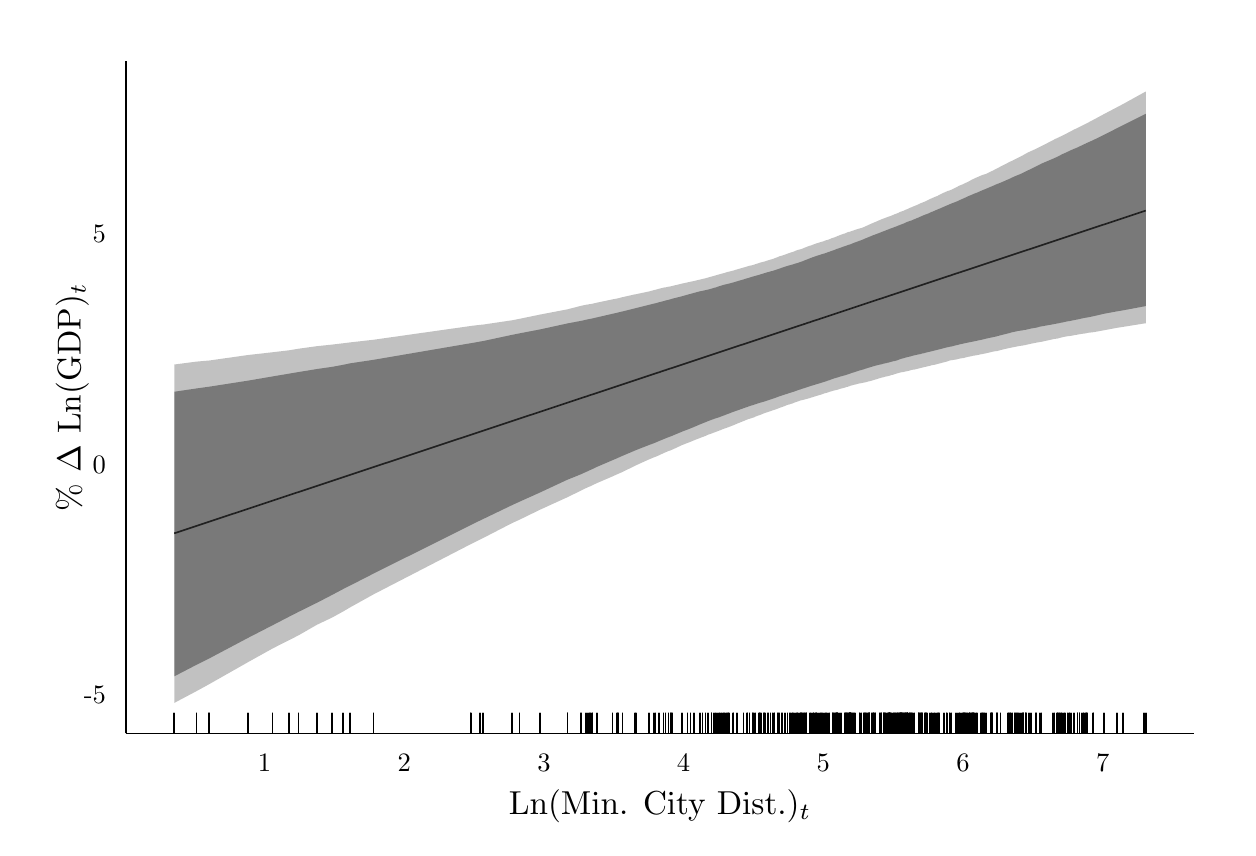
\begin{tikzpicture}[x=1pt,y=1pt]
\definecolor[named]{fillColor}{rgb}{1.00,1.00,1.00}
\path[use as bounding box,fill=fillColor,fill opacity=0.00] (0,0) rectangle (433.62,289.08);
\begin{scope}
\path[clip] (  0.00,  0.00) rectangle (433.62,289.08);
\definecolor[named]{drawColor}{rgb}{1.00,1.00,1.00}
\definecolor[named]{fillColor}{rgb}{1.00,1.00,1.00}

\path[draw=drawColor,line width= 0.6pt,line join=round,line cap=round,fill=fillColor] (  0.00,  0.00) rectangle (433.62,289.08);
\end{scope}
\begin{scope}
\path[clip] ( 35.42, 34.03) rectangle (421.57,277.03);
\definecolor[named]{fillColor}{rgb}{1.00,1.00,1.00}

\path[fill=fillColor] ( 35.42, 34.03) rectangle (421.57,277.03);
\definecolor[named]{drawColor}{rgb}{0.00,0.00,0.00}

\path[draw=drawColor,line width= 0.6pt,line join=round] ( 52.97,106.37) --
	( 61.01,109.04) --
	( 65.48,110.52) --
	( 65.62,110.57) --
	( 79.64,115.23) --
	( 88.50,118.17) --
	( 94.41,120.14) --
	( 97.84,121.27) --
	(104.50,123.49) --
	(110.01,125.32) --
	(113.94,126.62) --
	(116.56,127.49) --
	(124.94,130.28) --
	(160.01,141.93) --
	(160.15,141.97) --
	(163.56,143.10) --
	(164.50,143.42) --
	(175.08,146.93) --
	(177.68,147.80) --
	(185.12,150.27) --
	(195.04,153.56) --
	(195.05,153.57) --
	(199.79,155.14) --
	(200.09,155.24) --
	(201.70,155.77) --
	(202.42,156.01) --
	(203.15,156.26) --
	(203.24,156.29) --
	(203.92,156.51) --
	(204.08,156.56) --
	(205.70,157.10) --
	(211.30,158.97) --
	(213.02,159.54) --
	(213.22,159.60) --
	(213.28,159.62) --
	(214.88,160.15) --
	(219.39,161.65) --
	(219.87,161.81) --
	(224.51,163.35) --
	(226.38,163.97) --
	(226.89,164.14) --
	(228.22,164.58) --
	(229.80,165.11) --
	(230.53,165.35) --
	(231.54,165.69) --
	(232.29,165.94) --
	(232.55,166.02) --
	(232.60,166.04) --
	(233.03,166.18) --
	(236.50,167.34) --
	(238.44,167.98) --
	(239.50,168.33) --
	(240.76,168.75) --
	(242.87,169.45) --
	(243.82,169.77) --
	(244.87,170.11) --
	(245.90,170.46) --
	(247.14,170.87) --
	(247.15,170.87) --
	(248.00,171.16) --
	(248.59,171.35) --
	(249.15,171.54) --
	(249.91,171.79) --
	(250.14,171.87) --
	(250.71,172.06) --
	(251.21,172.22) --
	(251.61,172.35) --
	(251.88,172.44) --
	(252.52,172.66) --
	(252.98,172.81) --
	(253.12,172.85) --
	(253.36,172.94) --
	(254.91,173.45) --
	(255.02,173.49) --
	(256.32,173.92) --
	(258.61,174.68) --
	(260.03,175.15) --
	(260.14,175.19) --
	(260.80,175.41) --
	(261.97,175.79) --
	(262.19,175.87) --
	(262.48,175.96) --
	(262.99,176.14) --
	(264.29,176.57) --
	(264.50,176.64) --
	(264.53,176.65) --
	(264.97,176.79) --
	(266.10,177.17) --
	(266.13,177.18) --
	(266.44,177.28) --
	(267.28,177.56) --
	(267.71,177.70) --
	(268.38,177.92) --
	(269.11,178.17) --
	(269.74,178.38) --
	(269.87,178.42) --
	(271.02,178.80) --
	(271.10,178.83) --
	(271.68,179.02) --
	(272.40,179.26) --
	(272.79,179.39) --
	(273.63,179.67) --
	(274.52,179.96) --
	(275.28,180.22) --
	(275.59,180.32) --
	(276.13,180.50) --
	(276.31,180.56) --
	(276.77,180.71) --
	(277.30,180.89) --
	(277.98,181.12) --
	(278.04,181.13) --
	(278.45,181.27) --
	(279.17,181.51) --
	(279.30,181.55) --
	(279.52,181.62) --
	(279.66,181.67) --
	(279.69,181.68) --
	(280.15,181.83) --
	(280.53,181.96) --
	(280.72,182.02) --
	(281.20,182.18) --
	(281.36,182.24) --
	(281.45,182.27) --
	(282.80,182.71) --
	(283.05,182.80) --
	(283.89,183.08) --
	(283.98,183.11) --
	(284.07,183.14) --
	(284.62,183.32) --
	(284.86,183.40) --
	(285.03,183.46) --
	(285.13,183.49) --
	(286.00,183.78) --
	(286.57,183.97) --
	(286.59,183.98) --
	(287.25,184.19) --
	(287.81,184.38) --
	(288.54,184.62) --
	(288.59,184.64) --
	(289.22,184.85) --
	(289.76,185.03) --
	(290.76,185.36) --
	(290.86,185.39) --
	(291.20,185.51) --
	(291.32,185.54) --
	(291.81,185.71) --
	(291.88,185.73) --
	(292.21,185.84) --
	(292.36,185.89) --
	(292.42,185.91) --
	(292.49,185.93) --
	(292.51,185.94) --
	(292.62,185.98) --
	(293.21,186.17) --
	(293.91,186.41) --
	(295.25,186.85) --
	(295.45,186.92) --
	(295.51,186.94) --
	(295.93,187.08) --
	(295.99,187.10) --
	(296.10,187.13) --
	(296.47,187.26) --
	(296.65,187.32) --
	(296.99,187.43) --
	(297.01,187.43) --
	(297.04,187.45) --
	(297.05,187.45) --
	(297.09,187.46) --
	(297.13,187.47) --
	(297.22,187.51) --
	(297.31,187.53) --
	(297.31,187.53) --
	(297.71,187.67) --
	(297.96,187.75) --
	(298.34,187.88) --
	(298.57,187.95) --
	(299.04,188.11) --
	(300.58,188.62) --
	(300.69,188.66) --
	(301.32,188.87) --
	(302.10,189.13) --
	(302.23,189.17) --
	(302.50,189.26) --
	(302.82,189.36) --
	(302.98,189.42) --
	(303.49,189.59) --
	(303.87,189.71) --
	(304.04,189.77) --
	(304.05,189.77) --
	(304.17,189.82) --
	(304.21,189.83) --
	(304.88,190.05) --
	(305.44,190.24) --
	(305.52,190.26) --
	(305.61,190.29) --
	(305.86,190.37) --
	(306.19,190.49) --
	(306.32,190.53) --
	(307.91,191.06) --
	(307.96,191.07) --
	(308.47,191.24) --
	(308.57,191.27) --
	(309.22,191.49) --
	(309.44,191.56) --
	(309.51,191.59) --
	(309.67,191.64) --
	(310.00,191.75) --
	(310.25,191.83) --
	(310.76,192.00) --
	(310.92,192.06) --
	(311.04,192.09) --
	(311.16,192.14) --
	(311.41,192.22) --
	(311.41,192.22) --
	(311.44,192.23) --
	(311.54,192.26) --
	(311.68,192.31) --
	(311.68,192.31) --
	(311.88,192.38) --
	(312.22,192.49) --
	(312.92,192.72) --
	(313.12,192.79) --
	(313.27,192.84) --
	(313.53,192.93) --
	(313.83,193.02) --
	(314.24,193.16) --
	(314.31,193.18) --
	(314.45,193.23) --
	(314.63,193.29) --
	(315.00,193.41) --
	(315.21,193.48) --
	(315.23,193.49) --
	(315.37,193.53) --
	(315.48,193.57) --
	(315.51,193.58) --
	(315.62,193.62) --
	(315.70,193.64) --
	(315.79,193.67) --
	(316.13,193.79) --
	(316.22,193.82) --
	(316.38,193.87) --
	(316.61,193.95) --
	(316.93,194.05) --
	(317.07,194.10) --
	(317.20,194.14) --
	(317.36,194.20) --
	(317.75,194.33) --
	(317.76,194.33) --
	(317.79,194.34) --
	(317.86,194.36) --
	(317.89,194.37) --
	(317.98,194.40) --
	(318.43,194.55) --
	(318.60,194.61) --
	(318.85,194.69) --
	(319.11,194.78) --
	(319.21,194.81) --
	(319.52,194.91) --
	(319.81,195.01) --
	(320.44,195.22) --
	(321.85,195.69) --
	(321.91,195.71) --
	(322.04,195.75) --
	(322.30,195.84) --
	(322.60,195.94) --
	(322.75,195.99) --
	(323.02,196.08) --
	(323.10,196.10) --
	(323.28,196.16) --
	(324.05,196.42) --
	(324.42,196.54) --
	(324.61,196.60) --
	(324.72,196.64) --
	(325.08,196.76) --
	(325.99,197.06) --
	(326.58,197.26) --
	(326.72,197.31) --
	(327.61,197.60) --
	(327.91,197.70) --
	(328.67,197.95) --
	(328.94,198.04) --
	(329.07,198.09) --
	(329.52,198.24) --
	(331.17,198.78) --
	(332.00,199.06) --
	(332.27,199.15) --
	(333.07,199.42) --
	(333.19,199.45) --
	(333.76,199.64) --
	(335.51,200.23) --
	(336.07,200.41) --
	(336.75,200.64) --
	(336.88,200.68) --
	(337.54,200.90) --
	(337.92,201.03) --
	(338.29,201.15) --
	(338.32,201.16) --
	(338.37,201.17) --
	(338.79,201.32) --
	(338.87,201.34) --
	(339.41,201.52) --
	(339.54,201.56) --
	(340.26,201.80) --
	(340.28,201.81) --
	(340.36,201.84) --
	(340.58,201.91) --
	(340.90,202.02) --
	(341.07,202.07) --
	(341.38,202.18) --
	(341.48,202.21) --
	(341.53,202.23) --
	(341.57,202.24) --
	(342.00,202.38) --
	(342.06,202.40) --
	(342.60,202.58) --
	(342.92,202.69) --
	(344.39,203.18) --
	(344.81,203.31) --
	(345.03,203.39) --
	(345.51,203.55) --
	(345.56,203.56) --
	(346.27,203.80) --
	(348.09,204.40) --
	(348.19,204.44) --
	(348.32,204.48) --
	(348.52,204.55) --
	(348.65,204.59) --
	(350.04,205.05) --
	(350.29,205.13) --
	(350.39,205.17) --
	(351.49,205.53) --
	(354.19,206.43) --
	(354.41,206.50) --
	(354.96,206.69) --
	(354.99,206.69) --
	(355.28,206.79) --
	(355.84,206.98) --
	(356.71,207.27) --
	(356.75,207.28) --
	(357.50,207.53) --
	(357.53,207.54) --
	(358.04,207.71) --
	(358.62,207.90) --
	(359.31,208.13) --
	(359.62,208.23) --
	(359.75,208.28) --
	(359.85,208.31) --
	(360.61,208.56) --
	(360.64,208.57) --
	(360.71,208.60) --
	(361.91,208.99) --
	(362.60,209.22) --
	(364.24,209.77) --
	(364.46,209.84) --
	(365.70,210.25) --
	(366.29,210.45) --
	(370.53,211.86) --
	(371.02,212.02) --
	(372.06,212.37) --
	(372.07,212.37) --
	(372.38,212.47) --
	(372.60,212.54) --
	(372.90,212.65) --
	(373.16,212.73) --
	(373.53,212.86) --
	(373.80,212.94) --
	(374.46,213.16) --
	(374.81,213.28) --
	(375.77,213.60) --
	(376.36,213.80) --
	(376.51,213.85) --
	(376.93,213.98) --
	(378.03,214.35) --
	(379.36,214.79) --
	(379.36,214.79) --
	(380.09,215.03) --
	(380.12,215.04) --
	(381.03,215.35) --
	(381.47,215.49) --
	(381.75,215.58) --
	(382.36,215.79) --
	(382.44,215.82) --
	(382.57,215.86) --
	(383.02,216.01) --
	(385.04,216.68) --
	(385.16,216.72) --
	(388.87,217.95) --
	(393.56,219.51) --
	(395.71,220.22) --
	(403.26,222.73) --
	(404.02,222.98);
\definecolor[named]{fillColor}{rgb}{0.20,0.20,0.20}

\path[fill=fillColor,fill opacity=0.30] ( 52.97,167.36) --
	( 61.01,168.41) --
	( 65.48,168.80) --
	( 65.62,168.81) --
	( 79.64,170.79) --
	( 88.50,171.79) --
	( 94.41,172.49) --
	( 97.84,173.06) --
	(104.50,173.98) --
	(110.01,174.56) --
	(113.94,175.03) --
	(116.56,175.36) --
	(124.94,176.30) --
	(160.01,181.27) --
	(160.15,181.30) --
	(163.56,181.70) --
	(164.50,181.78) --
	(175.08,183.35) --
	(177.68,183.86) --
	(185.12,185.40) --
	(195.04,187.30) --
	(195.05,187.30) --
	(199.79,188.52) --
	(200.09,188.60) --
	(201.70,188.94) --
	(202.42,189.05) --
	(203.15,189.18) --
	(203.24,189.19) --
	(203.92,189.29) --
	(204.08,189.32) --
	(205.70,189.71) --
	(211.30,190.89) --
	(213.02,191.21) --
	(213.22,191.26) --
	(213.28,191.27) --
	(214.88,191.68) --
	(219.39,192.70) --
	(219.87,192.77) --
	(224.51,193.76) --
	(226.38,194.26) --
	(226.89,194.38) --
	(228.22,194.75) --
	(229.80,195.15) --
	(230.53,195.25) --
	(231.54,195.47) --
	(232.29,195.59) --
	(232.55,195.66) --
	(232.60,195.67) --
	(233.03,195.77) --
	(236.50,196.61) --
	(238.44,197.03) --
	(239.50,197.27) --
	(240.76,197.54) --
	(242.87,198.03) --
	(243.82,198.26) --
	(244.87,198.51) --
	(245.90,198.81) --
	(247.14,199.15) --
	(247.15,199.15) --
	(248.00,199.39) --
	(248.59,199.55) --
	(249.15,199.72) --
	(249.91,199.94) --
	(250.14,200.00) --
	(250.71,200.16) --
	(251.21,200.29) --
	(251.61,200.40) --
	(251.88,200.46) --
	(252.52,200.69) --
	(252.98,200.84) --
	(253.12,200.86) --
	(253.36,200.89) --
	(254.91,201.29) --
	(255.02,201.32) --
	(256.32,201.72) --
	(258.61,202.38) --
	(260.03,202.80) --
	(260.14,202.84) --
	(260.80,203.04) --
	(261.97,203.27) --
	(262.19,203.35) --
	(262.48,203.44) --
	(262.99,203.62) --
	(264.29,204.03) --
	(264.50,204.10) --
	(264.53,204.11) --
	(264.97,204.25) --
	(266.10,204.54) --
	(266.13,204.55) --
	(266.44,204.61) --
	(267.28,204.93) --
	(267.71,205.05) --
	(268.38,205.26) --
	(269.11,205.45) --
	(269.74,205.69) --
	(269.87,205.74) --
	(271.02,206.18) --
	(271.10,206.22) --
	(271.68,206.47) --
	(272.40,206.66) --
	(272.79,206.78) --
	(273.63,207.07) --
	(274.52,207.40) --
	(275.28,207.68) --
	(275.59,207.78) --
	(276.13,207.95) --
	(276.31,207.99) --
	(276.77,208.14) --
	(277.30,208.37) --
	(277.98,208.66) --
	(278.04,208.68) --
	(278.45,208.79) --
	(279.17,208.98) --
	(279.30,209.02) --
	(279.52,209.08) --
	(279.66,209.14) --
	(279.69,209.14) --
	(280.15,209.31) --
	(280.53,209.48) --
	(280.72,209.56) --
	(281.20,209.75) --
	(281.36,209.82) --
	(281.45,209.85) --
	(282.80,210.34) --
	(283.05,210.37) --
	(283.89,210.70) --
	(283.98,210.74) --
	(284.07,210.78) --
	(284.62,210.98) --
	(284.86,211.08) --
	(285.03,211.13) --
	(285.13,211.16) --
	(286.00,211.42) --
	(286.57,211.61) --
	(286.59,211.61) --
	(287.25,211.79) --
	(287.81,211.98) --
	(288.54,212.28) --
	(288.59,212.29) --
	(289.22,212.44) --
	(289.76,212.64) --
	(290.76,213.08) --
	(290.86,213.13) --
	(291.20,213.21) --
	(291.32,213.21) --
	(291.81,213.42) --
	(291.88,213.46) --
	(292.21,213.58) --
	(292.36,213.65) --
	(292.42,213.69) --
	(292.49,213.72) --
	(292.51,213.74) --
	(292.62,213.79) --
	(293.21,213.98) --
	(293.91,214.28) --
	(295.25,214.70) --
	(295.45,214.78) --
	(295.51,214.81) --
	(295.93,215.00) --
	(295.99,215.02) --
	(296.10,215.06) --
	(296.47,215.21) --
	(296.65,215.26) --
	(296.99,215.30) --
	(297.01,215.30) --
	(297.04,215.31) --
	(297.05,215.31) --
	(297.09,215.32) --
	(297.13,215.34) --
	(297.22,215.39) --
	(297.31,215.44) --
	(297.31,215.44) --
	(297.71,215.55) --
	(297.96,215.64) --
	(298.34,215.77) --
	(298.57,215.86) --
	(299.04,216.04) --
	(300.58,216.50) --
	(300.69,216.54) --
	(301.32,216.72) --
	(302.10,216.99) --
	(302.23,217.04) --
	(302.50,217.16) --
	(302.82,217.32) --
	(302.98,217.40) --
	(303.49,217.63) --
	(303.87,217.81) --
	(304.04,217.89) --
	(304.05,217.89) --
	(304.17,217.95) --
	(304.21,217.97) --
	(304.88,218.27) --
	(305.44,218.51) --
	(305.52,218.55) --
	(305.61,218.58) --
	(305.86,218.68) --
	(306.19,218.81) --
	(306.32,218.86) --
	(307.91,219.57) --
	(307.96,219.60) --
	(308.47,219.81) --
	(308.57,219.85) --
	(309.22,220.10) --
	(309.44,220.18) --
	(309.51,220.20) --
	(309.67,220.25) --
	(310.00,220.39) --
	(310.25,220.47) --
	(310.76,220.68) --
	(310.92,220.74) --
	(311.04,220.77) --
	(311.16,220.82) --
	(311.41,220.90) --
	(311.41,220.90) --
	(311.44,220.91) --
	(311.54,220.94) --
	(311.68,220.98) --
	(311.68,220.99) --
	(311.88,221.05) --
	(312.22,221.19) --
	(312.92,221.49) --
	(313.12,221.57) --
	(313.27,221.65) --
	(313.53,221.73) --
	(313.83,221.83) --
	(314.24,222.00) --
	(314.31,222.04) --
	(314.45,222.11) --
	(314.63,222.16) --
	(315.00,222.37) --
	(315.21,222.46) --
	(315.23,222.47) --
	(315.37,222.52) --
	(315.48,222.56) --
	(315.51,222.58) --
	(315.62,222.62) --
	(315.70,222.64) --
	(315.79,222.66) --
	(316.13,222.81) --
	(316.22,222.83) --
	(316.38,222.87) --
	(316.61,222.95) --
	(316.93,223.12) --
	(317.07,223.18) --
	(317.20,223.26) --
	(317.36,223.33) --
	(317.75,223.47) --
	(317.76,223.47) --
	(317.79,223.49) --
	(317.86,223.53) --
	(317.89,223.54) --
	(317.98,223.58) --
	(318.43,223.78) --
	(318.60,223.85) --
	(318.85,224.00) --
	(319.11,224.09) --
	(319.21,224.11) --
	(319.52,224.25) --
	(319.81,224.40) --
	(320.44,224.64) --
	(321.85,225.23) --
	(321.91,225.27) --
	(322.04,225.35) --
	(322.30,225.47) --
	(322.60,225.60) --
	(322.75,225.66) --
	(323.02,225.77) --
	(323.10,225.80) --
	(323.28,225.87) --
	(324.05,226.17) --
	(324.42,226.34) --
	(324.61,226.43) --
	(324.72,226.50) --
	(325.08,226.65) --
	(325.99,227.12) --
	(326.58,227.38) --
	(326.72,227.44) --
	(327.61,227.83) --
	(327.91,227.96) --
	(328.67,228.25) --
	(328.94,228.38) --
	(329.07,228.46) --
	(329.52,228.70) --
	(331.17,229.50) --
	(332.00,229.87) --
	(332.27,230.00) --
	(333.07,230.25) --
	(333.19,230.29) --
	(333.76,230.52) --
	(335.51,231.36) --
	(336.07,231.68) --
	(336.75,232.03) --
	(336.88,232.07) --
	(337.54,232.34) --
	(337.92,232.47) --
	(338.29,232.66) --
	(338.32,232.68) --
	(338.37,232.70) --
	(338.79,232.94) --
	(338.87,232.97) --
	(339.41,233.19) --
	(339.54,233.26) --
	(340.26,233.63) --
	(340.28,233.64) --
	(340.36,233.69) --
	(340.58,233.82) --
	(340.90,234.00) --
	(341.07,234.09) --
	(341.38,234.25) --
	(341.48,234.29) --
	(341.53,234.32) --
	(341.57,234.33) --
	(342.00,234.53) --
	(342.06,234.56) --
	(342.60,234.82) --
	(342.92,234.94) --
	(344.39,235.59) --
	(344.81,235.76) --
	(345.03,235.85) --
	(345.51,236.00) --
	(345.56,236.01) --
	(346.27,236.21) --
	(348.09,237.11) --
	(348.19,237.16) --
	(348.32,237.23) --
	(348.52,237.32) --
	(348.65,237.36) --
	(350.04,238.11) --
	(350.29,238.22) --
	(350.39,238.27) --
	(351.49,238.86) --
	(354.19,240.24) --
	(354.41,240.37) --
	(354.96,240.65) --
	(354.99,240.67) --
	(355.28,240.79) --
	(355.84,241.02) --
	(356.71,241.48) --
	(356.75,241.51) --
	(357.50,241.86) --
	(357.53,241.87) --
	(358.04,242.13) --
	(358.62,242.42) --
	(359.31,242.81) --
	(359.62,242.94) --
	(359.75,243.03) --
	(359.85,243.09) --
	(360.61,243.54) --
	(360.64,243.55) --
	(360.71,243.59) --
	(361.91,244.20) --
	(362.60,244.50) --
	(364.24,245.24) --
	(364.46,245.35) --
	(365.70,245.99) --
	(366.29,246.26) --
	(370.53,248.44) --
	(371.02,248.71) --
	(372.06,249.22) --
	(372.07,249.22) --
	(372.38,249.33) --
	(372.60,249.45) --
	(372.90,249.61) --
	(373.16,249.73) --
	(373.53,249.89) --
	(373.80,250.04) --
	(374.46,250.35) --
	(374.81,250.52) --
	(375.77,251.03) --
	(376.36,251.34) --
	(376.51,251.43) --
	(376.93,251.64) --
	(378.03,252.22) --
	(379.36,252.85) --
	(379.36,252.86) --
	(380.09,253.22) --
	(380.12,253.24) --
	(381.03,253.71) --
	(381.47,253.91) --
	(381.75,254.05) --
	(382.36,254.37) --
	(382.44,254.41) --
	(382.57,254.46) --
	(383.02,254.69) --
	(385.04,255.76) --
	(385.16,255.82) --
	(388.87,257.82) --
	(393.56,260.29) --
	(395.71,261.42) --
	(403.26,265.59) --
	(404.02,265.99) --
	(404.02,182.27) --
	(403.26,182.16) --
	(395.71,180.94) --
	(393.56,180.61) --
	(388.87,179.73) --
	(385.16,179.04) --
	(385.04,179.03) --
	(383.02,178.81) --
	(382.57,178.70) --
	(382.44,178.65) --
	(382.36,178.61) --
	(381.75,178.55) --
	(381.47,178.49) --
	(381.03,178.47) --
	(380.12,178.30) --
	(380.09,178.30) --
	(379.36,178.16) --
	(379.36,178.16) --
	(378.03,177.94) --
	(376.93,177.72) --
	(376.51,177.66) --
	(376.36,177.65) --
	(375.77,177.59) --
	(374.81,177.41) --
	(374.46,177.37) --
	(373.80,177.19) --
	(373.53,177.12) --
	(373.16,177.03) --
	(372.90,176.96) --
	(372.60,176.88) --
	(372.38,176.82) --
	(372.07,176.74) --
	(372.06,176.74) --
	(371.02,176.61) --
	(370.53,176.50) --
	(366.29,175.56) --
	(365.70,175.48) --
	(364.46,175.26) --
	(364.24,175.21) --
	(362.60,174.88) --
	(361.91,174.73) --
	(360.71,174.46) --
	(360.64,174.43) --
	(360.61,174.42) --
	(359.85,174.28) --
	(359.75,174.26) --
	(359.62,174.24) --
	(359.31,174.18) --
	(358.62,174.10) --
	(358.04,174.00) --
	(357.53,173.89) --
	(357.50,173.88) --
	(356.75,173.74) --
	(356.71,173.73) --
	(355.84,173.55) --
	(355.28,173.44) --
	(354.99,173.38) --
	(354.96,173.38) --
	(354.41,173.27) --
	(354.19,173.22) --
	(351.49,172.56) --
	(350.39,172.25) --
	(350.29,172.22) --
	(350.04,172.22) --
	(348.65,172.01) --
	(348.52,171.96) --
	(348.32,171.89) --
	(348.19,171.87) --
	(348.09,171.85) --
	(346.27,171.41) --
	(345.56,171.26) --
	(345.51,171.26) --
	(345.03,171.14) --
	(344.81,171.13) --
	(344.39,171.04) --
	(342.92,170.73) --
	(342.60,170.68) --
	(342.06,170.59) --
	(342.00,170.58) --
	(341.57,170.51) --
	(341.53,170.50) --
	(341.48,170.48) --
	(341.38,170.46) --
	(341.07,170.41) --
	(340.90,170.35) --
	(340.58,170.27) --
	(340.36,170.25) --
	(340.28,170.24) --
	(340.26,170.24) --
	(339.54,170.08) --
	(339.41,170.03) --
	(338.87,169.90) --
	(338.79,169.88) --
	(338.37,169.75) --
	(338.32,169.74) --
	(338.29,169.73) --
	(337.92,169.66) --
	(337.54,169.63) --
	(336.88,169.52) --
	(336.75,169.49) --
	(336.07,169.33) --
	(335.51,169.18) --
	(333.76,168.91) --
	(333.19,168.80) --
	(333.07,168.78) --
	(332.27,168.47) --
	(332.00,168.39) --
	(331.17,168.19) --
	(329.52,167.74) --
	(329.07,167.64) --
	(328.94,167.62) --
	(328.67,167.52) --
	(327.91,167.32) --
	(327.61,167.25) --
	(326.72,167.12) --
	(326.58,167.07) --
	(325.99,166.89) --
	(325.08,166.68) --
	(324.72,166.60) --
	(324.61,166.57) --
	(324.42,166.53) --
	(324.05,166.45) --
	(323.28,166.24) --
	(323.10,166.20) --
	(323.02,166.19) --
	(322.75,166.13) --
	(322.60,166.08) --
	(322.30,166.02) --
	(322.04,165.95) --
	(321.91,165.91) --
	(321.85,165.90) --
	(320.44,165.54) --
	(319.81,165.48) --
	(319.52,165.41) --
	(319.21,165.35) --
	(319.11,165.31) --
	(318.85,165.22) --
	(318.60,165.15) --
	(318.43,165.12) --
	(317.98,165.00) --
	(317.89,164.98) --
	(317.86,164.98) --
	(317.79,164.97) --
	(317.76,164.96) --
	(317.75,164.96) --
	(317.36,164.87) --
	(317.20,164.84) --
	(317.07,164.81) --
	(316.93,164.77) --
	(316.61,164.69) --
	(316.38,164.64) --
	(316.22,164.63) --
	(316.13,164.63) --
	(315.79,164.58) --
	(315.70,164.56) --
	(315.62,164.55) --
	(315.51,164.53) --
	(315.48,164.52) --
	(315.37,164.49) --
	(315.23,164.45) --
	(315.21,164.44) --
	(315.00,164.38) --
	(314.63,164.28) --
	(314.45,164.23) --
	(314.31,164.17) --
	(314.24,164.15) --
	(313.83,164.06) --
	(313.53,163.97) --
	(313.27,163.89) --
	(313.12,163.80) --
	(312.92,163.72) --
	(312.22,163.58) --
	(311.88,163.47) --
	(311.68,163.41) --
	(311.68,163.41) --
	(311.54,163.36) --
	(311.44,163.32) --
	(311.41,163.32) --
	(311.41,163.32) --
	(311.16,163.25) --
	(311.04,163.22) --
	(310.92,163.20) --
	(310.76,163.15) --
	(310.25,163.05) --
	(310.00,162.99) --
	(309.67,162.92) --
	(309.51,162.86) --
	(309.44,162.83) --
	(309.22,162.77) --
	(308.57,162.62) --
	(308.47,162.60) --
	(307.96,162.44) --
	(307.91,162.43) --
	(306.32,161.94) --
	(306.19,161.90) --
	(305.86,161.80) --
	(305.61,161.73) --
	(305.52,161.70) --
	(305.44,161.68) --
	(304.88,161.50) --
	(304.21,161.34) --
	(304.17,161.33) --
	(304.05,161.30) --
	(304.04,161.30) --
	(303.87,161.27) --
	(303.49,161.16) --
	(302.98,161.00) --
	(302.82,160.95) --
	(302.50,160.89) --
	(302.23,160.84) --
	(302.10,160.82) --
	(301.32,160.64) --
	(300.69,160.55) --
	(300.58,160.54) --
	(299.04,160.13) --
	(298.57,160.04) --
	(298.34,159.99) --
	(297.96,159.86) --
	(297.71,159.79) --
	(297.31,159.71) --
	(297.31,159.71) --
	(297.22,159.67) --
	(297.13,159.62) --
	(297.09,159.60) --
	(297.05,159.58) --
	(297.04,159.58) --
	(297.01,159.57) --
	(296.99,159.56) --
	(296.65,159.45) --
	(296.47,159.35) --
	(296.10,159.26) --
	(295.99,159.24) --
	(295.93,159.23) --
	(295.51,159.10) --
	(295.45,159.08) --
	(295.25,159.01) --
	(293.91,158.66) --
	(293.21,158.46) --
	(292.62,158.25) --
	(292.51,158.22) --
	(292.49,158.21) --
	(292.42,158.20) --
	(292.36,158.18) --
	(292.21,158.15) --
	(291.88,158.09) --
	(291.81,158.08) --
	(291.32,157.93) --
	(291.20,157.93) --
	(290.86,157.83) --
	(290.76,157.78) --
	(289.76,157.50) --
	(289.22,157.31) --
	(288.59,157.10) --
	(288.54,157.09) --
	(287.81,156.93) --
	(287.25,156.69) --
	(286.59,156.44) --
	(286.57,156.44) --
	(286.00,156.29) --
	(285.13,156.04) --
	(285.03,156.02) --
	(284.86,155.95) --
	(284.62,155.87) --
	(284.07,155.70) --
	(283.98,155.67) --
	(283.89,155.63) --
	(283.05,155.39) --
	(282.80,155.29) --
	(281.45,154.91) --
	(281.36,154.89) --
	(281.20,154.85) --
	(280.72,154.72) --
	(280.53,154.68) --
	(280.15,154.56) --
	(279.69,154.48) --
	(279.66,154.48) --
	(279.52,154.44) --
	(279.30,154.38) --
	(279.17,154.34) --
	(278.45,154.06) --
	(278.04,153.95) --
	(277.98,153.93) --
	(277.30,153.70) --
	(276.77,153.46) --
	(276.31,153.28) --
	(276.13,153.22) --
	(275.59,153.06) --
	(275.28,152.95) --
	(274.52,152.77) --
	(273.63,152.39) --
	(272.79,152.07) --
	(272.40,151.94) --
	(271.68,151.70) --
	(271.10,151.43) --
	(271.02,151.41) --
	(269.87,151.00) --
	(269.74,150.96) --
	(269.11,150.78) --
	(268.38,150.50) --
	(267.71,150.29) --
	(267.28,150.15) --
	(266.44,149.85) --
	(266.13,149.74) --
	(266.10,149.73) --
	(264.97,149.27) --
	(264.53,149.09) --
	(264.50,149.08) --
	(264.29,149.03) --
	(262.99,148.54) --
	(262.48,148.27) --
	(262.19,148.19) --
	(261.97,148.12) --
	(260.80,147.75) --
	(260.14,147.55) --
	(260.03,147.49) --
	(258.61,146.90) --
	(256.32,145.98) --
	(255.02,145.42) --
	(254.91,145.38) --
	(253.36,144.78) --
	(253.12,144.70) --
	(252.98,144.64) --
	(252.52,144.47) --
	(251.88,144.26) --
	(251.61,144.16) --
	(251.21,144.00) --
	(250.71,143.81) --
	(250.14,143.57) --
	(249.91,143.49) --
	(249.15,143.20) --
	(248.59,142.98) --
	(248.00,142.78) --
	(247.15,142.45) --
	(247.14,142.44) --
	(245.90,142.02) --
	(244.87,141.53) --
	(243.82,141.15) --
	(242.87,140.79) --
	(240.76,139.96) --
	(239.50,139.44) --
	(238.44,139.02) --
	(236.50,138.27) --
	(233.03,136.65) --
	(232.60,136.47) --
	(232.55,136.45) --
	(232.29,136.34) --
	(231.54,136.09) --
	(230.53,135.66) --
	(229.80,135.35) --
	(228.22,134.60) --
	(226.89,134.03) --
	(226.38,133.85) --
	(224.51,133.07) --
	(219.87,130.96) --
	(219.39,130.73) --
	(214.88,128.51) --
	(213.28,127.81) --
	(213.22,127.78) --
	(213.02,127.70) --
	(211.30,126.92) --
	(205.70,124.51) --
	(204.08,123.77) --
	(203.92,123.68) --
	(203.24,123.35) --
	(203.15,123.31) --
	(202.42,123.02) --
	(201.70,122.67) --
	(200.09,121.90) --
	(199.79,121.73) --
	(195.05,119.42) --
	(195.04,119.41) --
	(185.12,114.89) --
	(177.68,111.26) --
	(175.08,110.08) --
	(164.50,104.62) --
	(163.56,104.15) --
	(160.15,102.47) --
	(160.01,102.40) --
	(124.94, 84.29) --
	(116.56, 79.63) --
	(113.94, 78.09) --
	(110.01, 75.93) --
	(104.50, 73.31) --
	( 97.84, 69.48) --
	( 94.41, 67.75) --
	( 88.50, 64.75) --
	( 79.64, 59.82) --
	( 65.62, 51.87) --
	( 65.48, 51.79) --
	( 61.01, 49.34) --
	( 52.97, 45.08) --
	cycle;
\definecolor[named]{fillColor}{rgb}{0.20,0.20,0.20}

\path[fill=fillColor,fill opacity=0.50] ( 52.97,157.52) --
	( 61.01,158.71) --
	( 65.48,159.33) --
	( 65.62,159.35) --
	( 79.64,161.53) --
	( 88.50,163.05) --
	( 94.41,164.05) --
	( 97.84,164.63) --
	(104.50,165.72) --
	(110.01,166.51) --
	(113.94,167.24) --
	(116.56,167.79) --
	(124.94,169.05) --
	(160.01,175.04) --
	(160.15,175.05) --
	(163.56,175.67) --
	(164.50,175.82) --
	(175.08,178.09) --
	(177.68,178.61) --
	(185.12,180.03) --
	(195.04,182.20) --
	(195.05,182.20) --
	(199.79,183.10) --
	(200.09,183.15) --
	(201.70,183.53) --
	(202.42,183.68) --
	(203.15,183.82) --
	(203.24,183.84) --
	(203.92,183.98) --
	(204.08,184.00) --
	(205.70,184.39) --
	(211.30,185.68) --
	(213.02,186.07) --
	(213.22,186.12) --
	(213.28,186.14) --
	(214.88,186.52) --
	(219.39,187.64) --
	(219.87,187.75) --
	(224.51,188.92) --
	(226.38,189.39) --
	(226.89,189.48) --
	(228.22,189.88) --
	(229.80,190.26) --
	(230.53,190.49) --
	(231.54,190.73) --
	(232.29,190.94) --
	(232.55,191.02) --
	(232.60,191.04) --
	(233.03,191.16) --
	(236.50,192.03) --
	(238.44,192.60) --
	(239.50,192.87) --
	(240.76,193.23) --
	(242.87,193.80) --
	(243.82,193.97) --
	(244.87,194.22) --
	(245.90,194.45) --
	(247.14,194.78) --
	(247.15,194.78) --
	(248.00,195.06) --
	(248.59,195.19) --
	(249.15,195.38) --
	(249.91,195.68) --
	(250.14,195.72) --
	(250.71,195.90) --
	(251.21,196.07) --
	(251.61,196.16) --
	(251.88,196.25) --
	(252.52,196.37) --
	(252.98,196.48) --
	(253.12,196.53) --
	(253.36,196.58) --
	(254.91,197.00) --
	(255.02,197.02) --
	(256.32,197.42) --
	(258.61,198.09) --
	(260.03,198.53) --
	(260.14,198.54) --
	(260.80,198.76) --
	(261.97,199.13) --
	(262.19,199.18) --
	(262.48,199.25) --
	(262.99,199.41) --
	(264.29,199.74) --
	(264.50,199.84) --
	(264.53,199.86) --
	(264.97,199.98) --
	(266.10,200.32) --
	(266.13,200.33) --
	(266.44,200.43) --
	(267.28,200.69) --
	(267.71,200.79) --
	(268.38,200.99) --
	(269.11,201.16) --
	(269.74,201.38) --
	(269.87,201.40) --
	(271.02,201.80) --
	(271.10,201.83) --
	(271.68,202.00) --
	(272.40,202.28) --
	(272.79,202.41) --
	(273.63,202.69) --
	(274.52,202.98) --
	(275.28,203.20) --
	(275.59,203.27) --
	(276.13,203.43) --
	(276.31,203.47) --
	(276.77,203.63) --
	(277.30,203.79) --
	(277.98,204.00) --
	(278.04,204.00) --
	(278.45,204.12) --
	(279.17,204.40) --
	(279.30,204.44) --
	(279.52,204.50) --
	(279.66,204.55) --
	(279.69,204.56) --
	(280.15,204.72) --
	(280.53,204.89) --
	(280.72,204.98) --
	(281.20,205.18) --
	(281.36,205.23) --
	(281.45,205.24) --
	(282.80,205.79) --
	(283.05,205.89) --
	(283.89,206.20) --
	(283.98,206.21) --
	(284.07,206.25) --
	(284.62,206.45) --
	(284.86,206.51) --
	(285.03,206.59) --
	(285.13,206.64) --
	(286.00,206.89) --
	(286.57,207.08) --
	(286.59,207.10) --
	(287.25,207.30) --
	(287.81,207.46) --
	(288.54,207.69) --
	(288.59,207.71) --
	(289.22,207.96) --
	(289.76,208.14) --
	(290.76,208.49) --
	(290.86,208.52) --
	(291.20,208.64) --
	(291.32,208.69) --
	(291.81,208.87) --
	(291.88,208.91) --
	(292.21,209.05) --
	(292.36,209.11) --
	(292.42,209.13) --
	(292.49,209.15) --
	(292.51,209.16) --
	(292.62,209.22) --
	(293.21,209.38) --
	(293.91,209.64) --
	(295.25,210.12) --
	(295.45,210.17) --
	(295.51,210.19) --
	(295.93,210.34) --
	(295.99,210.37) --
	(296.10,210.42) --
	(296.47,210.53) --
	(296.65,210.60) --
	(296.99,210.70) --
	(297.01,210.71) --
	(297.04,210.72) --
	(297.05,210.72) --
	(297.09,210.73) --
	(297.13,210.74) --
	(297.22,210.77) --
	(297.31,210.80) --
	(297.31,210.80) --
	(297.71,210.96) --
	(297.96,211.07) --
	(298.34,211.23) --
	(298.57,211.33) --
	(299.04,211.48) --
	(300.58,212.07) --
	(300.69,212.11) --
	(301.32,212.32) --
	(302.10,212.65) --
	(302.23,212.71) --
	(302.50,212.86) --
	(302.82,212.96) --
	(302.98,213.02) --
	(303.49,213.24) --
	(303.87,213.38) --
	(304.04,213.46) --
	(304.05,213.46) --
	(304.17,213.52) --
	(304.21,213.54) --
	(304.88,213.80) --
	(305.44,214.06) --
	(305.52,214.08) --
	(305.61,214.12) --
	(305.86,214.20) --
	(306.19,214.32) --
	(306.32,214.36) --
	(307.91,214.96) --
	(307.96,214.99) --
	(308.47,215.19) --
	(308.57,215.23) --
	(309.22,215.49) --
	(309.44,215.58) --
	(309.51,215.60) --
	(309.67,215.66) --
	(310.00,215.78) --
	(310.25,215.88) --
	(310.76,216.10) --
	(310.92,216.15) --
	(311.04,216.19) --
	(311.16,216.24) --
	(311.41,216.35) --
	(311.41,216.36) --
	(311.44,216.37) --
	(311.54,216.40) --
	(311.68,216.46) --
	(311.68,216.46) --
	(311.88,216.53) --
	(312.22,216.64) --
	(312.92,216.90) --
	(313.12,216.98) --
	(313.27,217.05) --
	(313.53,217.12) --
	(313.83,217.24) --
	(314.24,217.40) --
	(314.31,217.42) --
	(314.45,217.49) --
	(314.63,217.59) --
	(315.00,217.69) --
	(315.21,217.81) --
	(315.23,217.82) --
	(315.37,217.86) --
	(315.48,217.91) --
	(315.51,217.92) --
	(315.62,217.95) --
	(315.70,217.98) --
	(315.79,218.02) --
	(316.13,218.15) --
	(316.22,218.18) --
	(316.38,218.25) --
	(316.61,218.33) --
	(316.93,218.48) --
	(317.07,218.54) --
	(317.20,218.60) --
	(317.36,218.68) --
	(317.75,218.86) --
	(317.76,218.87) --
	(317.79,218.88) --
	(317.86,218.90) --
	(317.89,218.91) --
	(317.98,218.95) --
	(318.43,219.10) --
	(318.60,219.15) --
	(318.85,219.23) --
	(319.11,219.34) --
	(319.21,219.36) --
	(319.52,219.46) --
	(319.81,219.61) --
	(320.44,219.87) --
	(321.85,220.46) --
	(321.91,220.48) --
	(322.04,220.54) --
	(322.30,220.65) --
	(322.60,220.80) --
	(322.75,220.85) --
	(323.02,220.98) --
	(323.10,221.01) --
	(323.28,221.10) --
	(324.05,221.40) --
	(324.42,221.57) --
	(324.61,221.63) --
	(324.72,221.66) --
	(325.08,221.77) --
	(325.99,222.17) --
	(326.58,222.47) --
	(326.72,222.50) --
	(327.61,222.87) --
	(327.91,223.02) --
	(328.67,223.32) --
	(328.94,223.47) --
	(329.07,223.53) --
	(329.52,223.68) --
	(331.17,224.41) --
	(332.00,224.77) --
	(332.27,224.86) --
	(333.07,225.24) --
	(333.19,225.28) --
	(333.76,225.52) --
	(335.51,226.18) --
	(336.07,226.42) --
	(336.75,226.75) --
	(336.88,226.82) --
	(337.54,227.09) --
	(337.92,227.27) --
	(338.29,227.44) --
	(338.32,227.46) --
	(338.37,227.49) --
	(338.79,227.66) --
	(338.87,227.69) --
	(339.41,227.95) --
	(339.54,228.00) --
	(340.26,228.35) --
	(340.28,228.35) --
	(340.36,228.38) --
	(340.58,228.46) --
	(340.90,228.61) --
	(341.07,228.67) --
	(341.38,228.80) --
	(341.48,228.85) --
	(341.53,228.88) --
	(341.57,228.90) --
	(342.00,229.08) --
	(342.06,229.11) --
	(342.60,229.32) --
	(342.92,229.41) --
	(344.39,230.06) --
	(344.81,230.26) --
	(345.03,230.35) --
	(345.51,230.53) --
	(345.56,230.55) --
	(346.27,230.84) --
	(348.09,231.63) --
	(348.19,231.66) --
	(348.32,231.71) --
	(348.52,231.79) --
	(348.65,231.84) --
	(350.04,232.48) --
	(350.29,232.58) --
	(350.39,232.61) --
	(351.49,233.03) --
	(354.19,234.20) --
	(354.41,234.28) --
	(354.96,234.53) --
	(354.99,234.54) --
	(355.28,234.70) --
	(355.84,234.97) --
	(356.71,235.37) --
	(356.75,235.39) --
	(357.50,235.70) --
	(357.53,235.71) --
	(358.04,235.90) --
	(358.62,236.15) --
	(359.31,236.46) --
	(359.62,236.61) --
	(359.75,236.69) --
	(359.85,236.75) --
	(360.61,237.12) --
	(360.64,237.13) --
	(360.71,237.18) --
	(361.91,237.72) --
	(362.60,238.04) --
	(364.24,238.88) --
	(364.46,239.00) --
	(365.70,239.62) --
	(366.29,239.93) --
	(370.53,241.73) --
	(371.02,241.94) --
	(372.06,242.43) --
	(372.07,242.43) --
	(372.38,242.60) --
	(372.60,242.71) --
	(372.90,242.85) --
	(373.16,243.00) --
	(373.53,243.19) --
	(373.80,243.33) --
	(374.46,243.64) --
	(374.81,243.78) --
	(375.77,244.22) --
	(376.36,244.50) --
	(376.51,244.59) --
	(376.93,244.79) --
	(378.03,245.25) --
	(379.36,245.80) --
	(379.36,245.80) --
	(380.09,246.17) --
	(380.12,246.18) --
	(381.03,246.59) --
	(381.47,246.80) --
	(381.75,246.94) --
	(382.36,247.23) --
	(382.44,247.28) --
	(382.57,247.34) --
	(383.02,247.55) --
	(385.04,248.44) --
	(385.16,248.51) --
	(388.87,250.32) --
	(393.56,252.71) --
	(395.71,253.79) --
	(403.26,257.56) --
	(404.02,257.95) --
	(404.02,188.48) --
	(403.26,188.33) --
	(395.71,186.92) --
	(393.56,186.56) --
	(388.87,185.69) --
	(385.16,184.82) --
	(385.04,184.80) --
	(383.02,184.39) --
	(382.57,184.31) --
	(382.44,184.30) --
	(382.36,184.29) --
	(381.75,184.16) --
	(381.47,184.11) --
	(381.03,184.04) --
	(380.12,183.81) --
	(380.09,183.80) --
	(379.36,183.64) --
	(379.36,183.64) --
	(378.03,183.40) --
	(376.93,183.15) --
	(376.51,183.06) --
	(376.36,183.05) --
	(375.77,182.97) --
	(374.81,182.77) --
	(374.46,182.70) --
	(373.80,182.52) --
	(373.53,182.49) --
	(373.16,182.43) --
	(372.90,182.36) --
	(372.60,182.28) --
	(372.38,182.23) --
	(372.07,182.19) --
	(372.06,182.19) --
	(371.02,182.00) --
	(370.53,181.89) --
	(366.29,181.14) --
	(365.70,181.03) --
	(364.46,180.67) --
	(364.24,180.65) --
	(362.60,180.37) --
	(361.91,180.21) --
	(360.71,179.92) --
	(360.64,179.91) --
	(360.61,179.91) --
	(359.85,179.80) --
	(359.75,179.78) --
	(359.62,179.75) --
	(359.31,179.68) --
	(358.62,179.58) --
	(358.04,179.52) --
	(357.53,179.41) --
	(357.50,179.40) --
	(356.75,179.23) --
	(356.71,179.22) --
	(355.84,179.05) --
	(355.28,178.90) --
	(354.99,178.79) --
	(354.96,178.78) --
	(354.41,178.64) --
	(354.19,178.60) --
	(351.49,177.92) --
	(350.39,177.61) --
	(350.29,177.59) --
	(350.04,177.51) --
	(348.65,177.21) --
	(348.52,177.18) --
	(348.32,177.15) --
	(348.19,177.12) --
	(348.09,177.09) --
	(346.27,176.71) --
	(345.56,176.53) --
	(345.51,176.51) --
	(345.03,176.39) --
	(344.81,176.34) --
	(344.39,176.25) --
	(342.92,175.94) --
	(342.60,175.88) --
	(342.06,175.75) --
	(342.00,175.73) --
	(341.57,175.65) --
	(341.53,175.64) --
	(341.48,175.64) --
	(341.38,175.62) --
	(341.07,175.54) --
	(340.90,175.51) --
	(340.58,175.45) --
	(340.36,175.41) --
	(340.28,175.40) --
	(340.26,175.39) --
	(339.54,175.25) --
	(339.41,175.22) --
	(338.87,175.11) --
	(338.79,175.10) --
	(338.37,175.01) --
	(338.32,174.99) --
	(338.29,174.98) --
	(337.92,174.87) --
	(337.54,174.80) --
	(336.88,174.67) --
	(336.75,174.64) --
	(336.07,174.44) --
	(335.51,174.32) --
	(333.76,173.87) --
	(333.19,173.78) --
	(333.07,173.75) --
	(332.27,173.58) --
	(332.00,173.51) --
	(331.17,173.30) --
	(329.52,172.87) --
	(329.07,172.77) --
	(328.94,172.73) --
	(328.67,172.67) --
	(327.91,172.46) --
	(327.61,172.39) --
	(326.72,172.17) --
	(326.58,172.14) --
	(325.99,172.00) --
	(325.08,171.78) --
	(324.72,171.70) --
	(324.61,171.67) --
	(324.42,171.61) --
	(324.05,171.49) --
	(323.28,171.35) --
	(323.10,171.31) --
	(323.02,171.29) --
	(322.75,171.18) --
	(322.60,171.15) --
	(322.30,171.10) --
	(322.04,171.03) --
	(321.91,171.01) --
	(321.85,171.00) --
	(320.44,170.69) --
	(319.81,170.53) --
	(319.52,170.45) --
	(319.21,170.37) --
	(319.11,170.34) --
	(318.85,170.26) --
	(318.60,170.22) --
	(318.43,170.18) --
	(317.98,170.05) --
	(317.89,170.02) --
	(317.86,170.01) --
	(317.79,169.99) --
	(317.76,169.99) --
	(317.75,169.99) --
	(317.36,169.90) --
	(317.20,169.85) --
	(317.07,169.82) --
	(316.93,169.79) --
	(316.61,169.68) --
	(316.38,169.60) --
	(316.22,169.57) --
	(316.13,169.55) --
	(315.79,169.46) --
	(315.70,169.44) --
	(315.62,169.41) --
	(315.51,169.37) --
	(315.48,169.36) --
	(315.37,169.32) --
	(315.23,169.28) --
	(315.21,169.27) --
	(315.00,169.20) --
	(314.63,169.05) --
	(314.45,168.98) --
	(314.31,168.94) --
	(314.24,168.90) --
	(313.83,168.77) --
	(313.53,168.69) --
	(313.27,168.63) --
	(313.12,168.61) --
	(312.92,168.58) --
	(312.22,168.40) --
	(311.88,168.29) --
	(311.68,168.25) --
	(311.68,168.25) --
	(311.54,168.22) --
	(311.44,168.18) --
	(311.41,168.17) --
	(311.41,168.17) --
	(311.16,168.09) --
	(311.04,168.07) --
	(310.92,168.05) --
	(310.76,168.02) --
	(310.25,167.88) --
	(310.00,167.83) --
	(309.67,167.75) --
	(309.51,167.72) --
	(309.44,167.71) --
	(309.22,167.66) --
	(308.57,167.46) --
	(308.47,167.44) --
	(307.96,167.34) --
	(307.91,167.34) --
	(306.32,166.93) --
	(306.19,166.90) --
	(305.86,166.81) --
	(305.61,166.74) --
	(305.52,166.71) --
	(305.44,166.69) --
	(304.88,166.51) --
	(304.21,166.30) --
	(304.17,166.30) --
	(304.05,166.26) --
	(304.04,166.26) --
	(303.87,166.21) --
	(303.49,166.10) --
	(302.98,165.93) --
	(302.82,165.89) --
	(302.50,165.78) --
	(302.23,165.67) --
	(302.10,165.62) --
	(301.32,165.40) --
	(300.69,165.24) --
	(300.58,165.20) --
	(299.04,164.69) --
	(298.57,164.54) --
	(298.34,164.48) --
	(297.96,164.38) --
	(297.71,164.30) --
	(297.31,164.13) --
	(297.31,164.13) --
	(297.22,164.10) --
	(297.13,164.08) --
	(297.09,164.07) --
	(297.05,164.05) --
	(297.04,164.05) --
	(297.01,164.04) --
	(296.99,164.03) --
	(296.65,163.91) --
	(296.47,163.85) --
	(296.10,163.73) --
	(295.99,163.69) --
	(295.93,163.67) --
	(295.51,163.54) --
	(295.45,163.52) --
	(295.25,163.45) --
	(293.91,163.09) --
	(293.21,162.89) --
	(292.62,162.68) --
	(292.51,162.66) --
	(292.49,162.65) --
	(292.42,162.63) --
	(292.36,162.61) --
	(292.21,162.56) --
	(291.88,162.48) --
	(291.81,162.46) --
	(291.32,162.32) --
	(291.20,162.27) --
	(290.86,162.16) --
	(290.76,162.12) --
	(289.76,161.73) --
	(289.22,161.57) --
	(288.59,161.34) --
	(288.54,161.32) --
	(287.81,161.08) --
	(287.25,160.92) --
	(286.59,160.70) --
	(286.57,160.70) --
	(286.00,160.52) --
	(285.13,160.28) --
	(285.03,160.25) --
	(284.86,160.19) --
	(284.62,160.11) --
	(284.07,159.94) --
	(283.98,159.91) --
	(283.89,159.89) --
	(283.05,159.64) --
	(282.80,159.57) --
	(281.45,159.12) --
	(281.36,159.08) --
	(281.20,159.03) --
	(280.72,158.84) --
	(280.53,158.80) --
	(280.15,158.71) --
	(279.69,158.55) --
	(279.66,158.54) --
	(279.52,158.48) --
	(279.30,158.40) --
	(279.17,158.36) --
	(278.45,158.13) --
	(278.04,157.99) --
	(277.98,157.96) --
	(277.30,157.71) --
	(276.77,157.53) --
	(276.31,157.40) --
	(276.13,157.34) --
	(275.59,157.16) --
	(275.28,157.07) --
	(274.52,156.81) --
	(273.63,156.52) --
	(272.79,156.25) --
	(272.40,156.11) --
	(271.68,155.88) --
	(271.10,155.68) --
	(271.02,155.65) --
	(269.87,155.20) --
	(269.74,155.17) --
	(269.11,154.96) --
	(268.38,154.71) --
	(267.71,154.49) --
	(267.28,154.34) --
	(266.44,154.07) --
	(266.13,153.97) --
	(266.10,153.96) --
	(264.97,153.64) --
	(264.53,153.52) --
	(264.50,153.51) --
	(264.29,153.45) --
	(262.99,153.00) --
	(262.48,152.85) --
	(262.19,152.74) --
	(261.97,152.68) --
	(260.80,152.32) --
	(260.14,152.06) --
	(260.03,152.03) --
	(258.61,151.54) --
	(256.32,150.72) --
	(255.02,150.28) --
	(254.91,150.24) --
	(253.36,149.63) --
	(253.12,149.55) --
	(252.98,149.50) --
	(252.52,149.32) --
	(251.88,149.06) --
	(251.61,148.94) --
	(251.21,148.84) --
	(250.71,148.65) --
	(250.14,148.41) --
	(249.91,148.31) --
	(249.15,148.07) --
	(248.59,147.93) --
	(248.00,147.70) --
	(247.15,147.40) --
	(247.14,147.39) --
	(245.90,146.93) --
	(244.87,146.49) --
	(243.82,146.09) --
	(242.87,145.70) --
	(240.76,144.79) --
	(239.50,144.28) --
	(238.44,143.86) --
	(236.50,143.12) --
	(233.03,141.67) --
	(232.60,141.48) --
	(232.55,141.46) --
	(232.29,141.37) --
	(231.54,141.09) --
	(230.53,140.70) --
	(229.80,140.39) --
	(228.22,139.75) --
	(226.89,139.17) --
	(226.38,138.96) --
	(224.51,138.27) --
	(219.87,136.46) --
	(219.39,136.25) --
	(214.88,134.34) --
	(213.28,133.63) --
	(213.22,133.61) --
	(213.02,133.50) --
	(211.30,132.78) --
	(205.70,130.38) --
	(204.08,129.58) --
	(203.92,129.52) --
	(203.24,129.24) --
	(203.15,129.19) --
	(202.42,128.83) --
	(201.70,128.52) --
	(200.09,127.78) --
	(199.79,127.65) --
	(195.05,125.74) --
	(195.04,125.74) --
	(185.12,121.11) --
	(177.68,117.77) --
	(175.08,116.58) --
	(164.50,111.49) --
	(163.56,111.05) --
	(160.15,109.37) --
	(160.01,109.30) --
	(124.94, 91.80) --
	(116.56, 87.52) --
	(113.94, 86.20) --
	(110.01, 84.11) --
	(104.50, 81.25) --
	( 97.84, 77.97) --
	( 94.41, 76.21) --
	( 88.50, 73.15) --
	( 79.64, 68.59) --
	( 65.62, 61.16) --
	( 65.48, 61.09) --
	( 61.01, 58.86) --
	( 52.97, 54.68) --
	cycle;

\path[draw=drawColor,line width= 0.6pt,line join=round,line cap=round] ( 52.97, 34.03) -- ( 52.97, 41.32);

\path[draw=drawColor,line width= 0.6pt,line join=round,line cap=round] ( 61.01, 34.03) -- ( 61.01, 41.32);

\path[draw=drawColor,line width= 0.6pt,line join=round,line cap=round] ( 65.48, 34.03) -- ( 65.48, 41.32);

\path[draw=drawColor,line width= 0.6pt,line join=round,line cap=round] ( 65.62, 34.03) -- ( 65.62, 41.32);

\path[draw=drawColor,line width= 0.6pt,line join=round,line cap=round] ( 79.64, 34.03) -- ( 79.64, 41.32);

\path[draw=drawColor,line width= 0.6pt,line join=round,line cap=round] ( 88.50, 34.03) -- ( 88.50, 41.32);

\path[draw=drawColor,line width= 0.6pt,line join=round,line cap=round] ( 94.41, 34.03) -- ( 94.41, 41.32);

\path[draw=drawColor,line width= 0.6pt,line join=round,line cap=round] ( 97.84, 34.03) -- ( 97.84, 41.32);

\path[draw=drawColor,line width= 0.6pt,line join=round,line cap=round] (104.50, 34.03) -- (104.50, 41.32);

\path[draw=drawColor,line width= 0.6pt,line join=round,line cap=round] (110.01, 34.03) -- (110.01, 41.32);

\path[draw=drawColor,line width= 0.6pt,line join=round,line cap=round] (113.94, 34.03) -- (113.94, 41.32);

\path[draw=drawColor,line width= 0.6pt,line join=round,line cap=round] (116.56, 34.03) -- (116.56, 41.32);

\path[draw=drawColor,line width= 0.6pt,line join=round,line cap=round] (124.94, 34.03) -- (124.94, 41.32);

\path[draw=drawColor,line width= 0.6pt,line join=round,line cap=round] (160.01, 34.03) -- (160.01, 41.32);

\path[draw=drawColor,line width= 0.6pt,line join=round,line cap=round] (160.15, 34.03) -- (160.15, 41.32);

\path[draw=drawColor,line width= 0.6pt,line join=round,line cap=round] (163.56, 34.03) -- (163.56, 41.32);

\path[draw=drawColor,line width= 0.6pt,line join=round,line cap=round] (164.50, 34.03) -- (164.50, 41.32);

\path[draw=drawColor,line width= 0.6pt,line join=round,line cap=round] (175.08, 34.03) -- (175.08, 41.32);

\path[draw=drawColor,line width= 0.6pt,line join=round,line cap=round] (177.68, 34.03) -- (177.68, 41.32);

\path[draw=drawColor,line width= 0.6pt,line join=round,line cap=round] (185.12, 34.03) -- (185.12, 41.32);

\path[draw=drawColor,line width= 0.6pt,line join=round,line cap=round] (195.04, 34.03) -- (195.04, 41.32);

\path[draw=drawColor,line width= 0.6pt,line join=round,line cap=round] (195.05, 34.03) -- (195.05, 41.32);

\path[draw=drawColor,line width= 0.6pt,line join=round,line cap=round] (199.79, 34.03) -- (199.79, 41.32);

\path[draw=drawColor,line width= 0.6pt,line join=round,line cap=round] (200.09, 34.03) -- (200.09, 41.32);

\path[draw=drawColor,line width= 0.6pt,line join=round,line cap=round] (201.70, 34.03) -- (201.70, 41.32);

\path[draw=drawColor,line width= 0.6pt,line join=round,line cap=round] (202.42, 34.03) -- (202.42, 41.32);

\path[draw=drawColor,line width= 0.6pt,line join=round,line cap=round] (203.15, 34.03) -- (203.15, 41.32);

\path[draw=drawColor,line width= 0.6pt,line join=round,line cap=round] (203.24, 34.03) -- (203.24, 41.32);

\path[draw=drawColor,line width= 0.6pt,line join=round,line cap=round] (203.92, 34.03) -- (203.92, 41.32);

\path[draw=drawColor,line width= 0.6pt,line join=round,line cap=round] (204.08, 34.03) -- (204.08, 41.32);

\path[draw=drawColor,line width= 0.6pt,line join=round,line cap=round] (205.70, 34.03) -- (205.70, 41.32);

\path[draw=drawColor,line width= 0.6pt,line join=round,line cap=round] (211.30, 34.03) -- (211.30, 41.32);

\path[draw=drawColor,line width= 0.6pt,line join=round,line cap=round] (213.02, 34.03) -- (213.02, 41.32);

\path[draw=drawColor,line width= 0.6pt,line join=round,line cap=round] (213.22, 34.03) -- (213.22, 41.32);

\path[draw=drawColor,line width= 0.6pt,line join=round,line cap=round] (213.28, 34.03) -- (213.28, 41.32);

\path[draw=drawColor,line width= 0.6pt,line join=round,line cap=round] (214.88, 34.03) -- (214.88, 41.32);

\path[draw=drawColor,line width= 0.6pt,line join=round,line cap=round] (219.39, 34.03) -- (219.39, 41.32);

\path[draw=drawColor,line width= 0.6pt,line join=round,line cap=round] (219.87, 34.03) -- (219.87, 41.32);

\path[draw=drawColor,line width= 0.6pt,line join=round,line cap=round] (224.51, 34.03) -- (224.51, 41.32);

\path[draw=drawColor,line width= 0.6pt,line join=round,line cap=round] (226.38, 34.03) -- (226.38, 41.32);

\path[draw=drawColor,line width= 0.6pt,line join=round,line cap=round] (226.89, 34.03) -- (226.89, 41.32);

\path[draw=drawColor,line width= 0.6pt,line join=round,line cap=round] (228.22, 34.03) -- (228.22, 41.32);

\path[draw=drawColor,line width= 0.6pt,line join=round,line cap=round] (229.80, 34.03) -- (229.80, 41.32);

\path[draw=drawColor,line width= 0.6pt,line join=round,line cap=round] (230.53, 34.03) -- (230.53, 41.32);

\path[draw=drawColor,line width= 0.6pt,line join=round,line cap=round] (231.54, 34.03) -- (231.54, 41.32);

\path[draw=drawColor,line width= 0.6pt,line join=round,line cap=round] (232.29, 34.03) -- (232.29, 41.32);

\path[draw=drawColor,line width= 0.6pt,line join=round,line cap=round] (232.55, 34.03) -- (232.55, 41.32);

\path[draw=drawColor,line width= 0.6pt,line join=round,line cap=round] (232.60, 34.03) -- (232.60, 41.32);

\path[draw=drawColor,line width= 0.6pt,line join=round,line cap=round] (233.03, 34.03) -- (233.03, 41.32);

\path[draw=drawColor,line width= 0.6pt,line join=round,line cap=round] (236.50, 34.03) -- (236.50, 41.32);

\path[draw=drawColor,line width= 0.6pt,line join=round,line cap=round] (238.44, 34.03) -- (238.44, 41.32);

\path[draw=drawColor,line width= 0.6pt,line join=round,line cap=round] (239.49, 34.03) -- (239.49, 41.32);

\path[draw=drawColor,line width= 0.6pt,line join=round,line cap=round] (240.76, 34.03) -- (240.76, 41.32);

\path[draw=drawColor,line width= 0.6pt,line join=round,line cap=round] (242.87, 34.03) -- (242.87, 41.32);

\path[draw=drawColor,line width= 0.6pt,line join=round,line cap=round] (243.82, 34.03) -- (243.82, 41.32);

\path[draw=drawColor,line width= 0.6pt,line join=round,line cap=round] (244.87, 34.03) -- (244.87, 41.32);

\path[draw=drawColor,line width= 0.6pt,line join=round,line cap=round] (245.90, 34.03) -- (245.90, 41.32);

\path[draw=drawColor,line width= 0.6pt,line join=round,line cap=round] (247.14, 34.03) -- (247.14, 41.32);

\path[draw=drawColor,line width= 0.6pt,line join=round,line cap=round] (247.15, 34.03) -- (247.15, 41.32);

\path[draw=drawColor,line width= 0.6pt,line join=round,line cap=round] (248.00, 34.03) -- (248.00, 41.32);

\path[draw=drawColor,line width= 0.6pt,line join=round,line cap=round] (248.59, 34.03) -- (248.59, 41.32);

\path[draw=drawColor,line width= 0.6pt,line join=round,line cap=round] (249.15, 34.03) -- (249.15, 41.32);

\path[draw=drawColor,line width= 0.6pt,line join=round,line cap=round] (249.91, 34.03) -- (249.91, 41.32);

\path[draw=drawColor,line width= 0.6pt,line join=round,line cap=round] (250.14, 34.03) -- (250.14, 41.32);

\path[draw=drawColor,line width= 0.6pt,line join=round,line cap=round] (250.71, 34.03) -- (250.71, 41.32);

\path[draw=drawColor,line width= 0.6pt,line join=round,line cap=round] (251.21, 34.03) -- (251.21, 41.32);

\path[draw=drawColor,line width= 0.6pt,line join=round,line cap=round] (251.61, 34.03) -- (251.61, 41.32);

\path[draw=drawColor,line width= 0.6pt,line join=round,line cap=round] (251.88, 34.03) -- (251.88, 41.32);

\path[draw=drawColor,line width= 0.6pt,line join=round,line cap=round] (252.52, 34.03) -- (252.52, 41.32);

\path[draw=drawColor,line width= 0.6pt,line join=round,line cap=round] (252.98, 34.03) -- (252.98, 41.32);

\path[draw=drawColor,line width= 0.6pt,line join=round,line cap=round] (253.12, 34.03) -- (253.12, 41.32);

\path[draw=drawColor,line width= 0.6pt,line join=round,line cap=round] (253.36, 34.03) -- (253.36, 41.32);

\path[draw=drawColor,line width= 0.6pt,line join=round,line cap=round] (254.91, 34.03) -- (254.91, 41.32);

\path[draw=drawColor,line width= 0.6pt,line join=round,line cap=round] (255.02, 34.03) -- (255.02, 41.32);

\path[draw=drawColor,line width= 0.6pt,line join=round,line cap=round] (256.32, 34.03) -- (256.32, 41.32);

\path[draw=drawColor,line width= 0.6pt,line join=round,line cap=round] (258.61, 34.03) -- (258.61, 41.32);

\path[draw=drawColor,line width= 0.6pt,line join=round,line cap=round] (260.03, 34.03) -- (260.03, 41.32);

\path[draw=drawColor,line width= 0.6pt,line join=round,line cap=round] (260.14, 34.03) -- (260.14, 41.32);

\path[draw=drawColor,line width= 0.6pt,line join=round,line cap=round] (260.80, 34.03) -- (260.80, 41.32);

\path[draw=drawColor,line width= 0.6pt,line join=round,line cap=round] (261.97, 34.03) -- (261.97, 41.32);

\path[draw=drawColor,line width= 0.6pt,line join=round,line cap=round] (262.19, 34.03) -- (262.19, 41.32);

\path[draw=drawColor,line width= 0.6pt,line join=round,line cap=round] (262.47, 34.03) -- (262.47, 41.32);

\path[draw=drawColor,line width= 0.6pt,line join=round,line cap=round] (262.99, 34.03) -- (262.99, 41.32);

\path[draw=drawColor,line width= 0.6pt,line join=round,line cap=round] (264.29, 34.03) -- (264.29, 41.32);

\path[draw=drawColor,line width= 0.6pt,line join=round,line cap=round] (264.50, 34.03) -- (264.50, 41.32);

\path[draw=drawColor,line width= 0.6pt,line join=round,line cap=round] (264.53, 34.03) -- (264.53, 41.32);

\path[draw=drawColor,line width= 0.6pt,line join=round,line cap=round] (264.97, 34.03) -- (264.97, 41.32);

\path[draw=drawColor,line width= 0.6pt,line join=round,line cap=round] (266.10, 34.03) -- (266.10, 41.32);

\path[draw=drawColor,line width= 0.6pt,line join=round,line cap=round] (266.13, 34.03) -- (266.13, 41.32);

\path[draw=drawColor,line width= 0.6pt,line join=round,line cap=round] (266.44, 34.03) -- (266.44, 41.32);

\path[draw=drawColor,line width= 0.6pt,line join=round,line cap=round] (267.28, 34.03) -- (267.28, 41.32);

\path[draw=drawColor,line width= 0.6pt,line join=round,line cap=round] (267.71, 34.03) -- (267.71, 41.32);

\path[draw=drawColor,line width= 0.6pt,line join=round,line cap=round] (268.38, 34.03) -- (268.38, 41.32);

\path[draw=drawColor,line width= 0.6pt,line join=round,line cap=round] (269.11, 34.03) -- (269.11, 41.32);

\path[draw=drawColor,line width= 0.6pt,line join=round,line cap=round] (269.74, 34.03) -- (269.74, 41.32);

\path[draw=drawColor,line width= 0.6pt,line join=round,line cap=round] (269.87, 34.03) -- (269.87, 41.32);

\path[draw=drawColor,line width= 0.6pt,line join=round,line cap=round] (271.02, 34.03) -- (271.02, 41.32);

\path[draw=drawColor,line width= 0.6pt,line join=round,line cap=round] (271.10, 34.03) -- (271.10, 41.32);

\path[draw=drawColor,line width= 0.6pt,line join=round,line cap=round] (271.68, 34.03) -- (271.68, 41.32);

\path[draw=drawColor,line width= 0.6pt,line join=round,line cap=round] (272.40, 34.03) -- (272.40, 41.32);

\path[draw=drawColor,line width= 0.6pt,line join=round,line cap=round] (272.79, 34.03) -- (272.79, 41.32);

\path[draw=drawColor,line width= 0.6pt,line join=round,line cap=round] (273.63, 34.03) -- (273.63, 41.32);

\path[draw=drawColor,line width= 0.6pt,line join=round,line cap=round] (274.52, 34.03) -- (274.52, 41.32);

\path[draw=drawColor,line width= 0.6pt,line join=round,line cap=round] (275.28, 34.03) -- (275.28, 41.32);

\path[draw=drawColor,line width= 0.6pt,line join=round,line cap=round] (275.59, 34.03) -- (275.59, 41.32);

\path[draw=drawColor,line width= 0.6pt,line join=round,line cap=round] (276.13, 34.03) -- (276.13, 41.32);

\path[draw=drawColor,line width= 0.6pt,line join=round,line cap=round] (276.31, 34.03) -- (276.31, 41.32);

\path[draw=drawColor,line width= 0.6pt,line join=round,line cap=round] (276.77, 34.03) -- (276.77, 41.32);

\path[draw=drawColor,line width= 0.6pt,line join=round,line cap=round] (277.30, 34.03) -- (277.30, 41.32);

\path[draw=drawColor,line width= 0.6pt,line join=round,line cap=round] (277.98, 34.03) -- (277.98, 41.32);

\path[draw=drawColor,line width= 0.6pt,line join=round,line cap=round] (278.04, 34.03) -- (278.04, 41.32);

\path[draw=drawColor,line width= 0.6pt,line join=round,line cap=round] (278.45, 34.03) -- (278.45, 41.32);

\path[draw=drawColor,line width= 0.6pt,line join=round,line cap=round] (279.17, 34.03) -- (279.17, 41.32);

\path[draw=drawColor,line width= 0.6pt,line join=round,line cap=round] (279.30, 34.03) -- (279.30, 41.32);

\path[draw=drawColor,line width= 0.6pt,line join=round,line cap=round] (279.52, 34.03) -- (279.52, 41.32);

\path[draw=drawColor,line width= 0.6pt,line join=round,line cap=round] (279.66, 34.03) -- (279.66, 41.32);

\path[draw=drawColor,line width= 0.6pt,line join=round,line cap=round] (279.69, 34.03) -- (279.69, 41.32);

\path[draw=drawColor,line width= 0.6pt,line join=round,line cap=round] (280.15, 34.03) -- (280.15, 41.32);

\path[draw=drawColor,line width= 0.6pt,line join=round,line cap=round] (280.53, 34.03) -- (280.53, 41.32);

\path[draw=drawColor,line width= 0.6pt,line join=round,line cap=round] (280.72, 34.03) -- (280.72, 41.32);

\path[draw=drawColor,line width= 0.6pt,line join=round,line cap=round] (281.20, 34.03) -- (281.20, 41.32);

\path[draw=drawColor,line width= 0.6pt,line join=round,line cap=round] (281.36, 34.03) -- (281.36, 41.32);

\path[draw=drawColor,line width= 0.6pt,line join=round,line cap=round] (281.45, 34.03) -- (281.45, 41.32);

\path[draw=drawColor,line width= 0.6pt,line join=round,line cap=round] (282.79, 34.03) -- (282.79, 41.32);

\path[draw=drawColor,line width= 0.6pt,line join=round,line cap=round] (283.05, 34.03) -- (283.05, 41.32);

\path[draw=drawColor,line width= 0.6pt,line join=round,line cap=round] (283.89, 34.03) -- (283.89, 41.32);

\path[draw=drawColor,line width= 0.6pt,line join=round,line cap=round] (283.98, 34.03) -- (283.98, 41.32);

\path[draw=drawColor,line width= 0.6pt,line join=round,line cap=round] (284.07, 34.03) -- (284.07, 41.32);

\path[draw=drawColor,line width= 0.6pt,line join=round,line cap=round] (284.63, 34.03) -- (284.63, 41.32);

\path[draw=drawColor,line width= 0.6pt,line join=round,line cap=round] (284.86, 34.03) -- (284.86, 41.32);

\path[draw=drawColor,line width= 0.6pt,line join=round,line cap=round] (285.03, 34.03) -- (285.03, 41.32);

\path[draw=drawColor,line width= 0.6pt,line join=round,line cap=round] (285.13, 34.03) -- (285.13, 41.32);

\path[draw=drawColor,line width= 0.6pt,line join=round,line cap=round] (286.00, 34.03) -- (286.00, 41.32);

\path[draw=drawColor,line width= 0.6pt,line join=round,line cap=round] (286.57, 34.03) -- (286.57, 41.32);

\path[draw=drawColor,line width= 0.6pt,line join=round,line cap=round] (286.59, 34.03) -- (286.59, 41.32);

\path[draw=drawColor,line width= 0.6pt,line join=round,line cap=round] (287.25, 34.03) -- (287.25, 41.32);

\path[draw=drawColor,line width= 0.6pt,line join=round,line cap=round] (287.81, 34.03) -- (287.81, 41.32);

\path[draw=drawColor,line width= 0.6pt,line join=round,line cap=round] (288.54, 34.03) -- (288.54, 41.32);

\path[draw=drawColor,line width= 0.6pt,line join=round,line cap=round] (288.59, 34.03) -- (288.59, 41.32);

\path[draw=drawColor,line width= 0.6pt,line join=round,line cap=round] (289.22, 34.03) -- (289.22, 41.32);

\path[draw=drawColor,line width= 0.6pt,line join=round,line cap=round] (289.76, 34.03) -- (289.76, 41.32);

\path[draw=drawColor,line width= 0.6pt,line join=round,line cap=round] (290.76, 34.03) -- (290.76, 41.32);

\path[draw=drawColor,line width= 0.6pt,line join=round,line cap=round] (290.86, 34.03) -- (290.86, 41.32);

\path[draw=drawColor,line width= 0.6pt,line join=round,line cap=round] (291.20, 34.03) -- (291.20, 41.32);

\path[draw=drawColor,line width= 0.6pt,line join=round,line cap=round] (291.32, 34.03) -- (291.32, 41.32);

\path[draw=drawColor,line width= 0.6pt,line join=round,line cap=round] (291.81, 34.03) -- (291.81, 41.32);

\path[draw=drawColor,line width= 0.6pt,line join=round,line cap=round] (291.88, 34.03) -- (291.88, 41.32);

\path[draw=drawColor,line width= 0.6pt,line join=round,line cap=round] (292.21, 34.03) -- (292.21, 41.32);

\path[draw=drawColor,line width= 0.6pt,line join=round,line cap=round] (292.36, 34.03) -- (292.36, 41.32);

\path[draw=drawColor,line width= 0.6pt,line join=round,line cap=round] (292.42, 34.03) -- (292.42, 41.32);

\path[draw=drawColor,line width= 0.6pt,line join=round,line cap=round] (292.49, 34.03) -- (292.49, 41.32);

\path[draw=drawColor,line width= 0.6pt,line join=round,line cap=round] (292.51, 34.03) -- (292.51, 41.32);

\path[draw=drawColor,line width= 0.6pt,line join=round,line cap=round] (292.62, 34.03) -- (292.62, 41.32);

\path[draw=drawColor,line width= 0.6pt,line join=round,line cap=round] (293.21, 34.03) -- (293.21, 41.32);

\path[draw=drawColor,line width= 0.6pt,line join=round,line cap=round] (293.91, 34.03) -- (293.91, 41.32);

\path[draw=drawColor,line width= 0.6pt,line join=round,line cap=round] (295.25, 34.03) -- (295.25, 41.32);

\path[draw=drawColor,line width= 0.6pt,line join=round,line cap=round] (295.45, 34.03) -- (295.45, 41.32);

\path[draw=drawColor,line width= 0.6pt,line join=round,line cap=round] (295.51, 34.03) -- (295.51, 41.32);

\path[draw=drawColor,line width= 0.6pt,line join=round,line cap=round] (295.93, 34.03) -- (295.93, 41.32);

\path[draw=drawColor,line width= 0.6pt,line join=round,line cap=round] (295.99, 34.03) -- (295.99, 41.32);

\path[draw=drawColor,line width= 0.6pt,line join=round,line cap=round] (296.10, 34.03) -- (296.10, 41.32);

\path[draw=drawColor,line width= 0.6pt,line join=round,line cap=round] (296.47, 34.03) -- (296.47, 41.32);

\path[draw=drawColor,line width= 0.6pt,line join=round,line cap=round] (296.65, 34.03) -- (296.65, 41.32);

\path[draw=drawColor,line width= 0.6pt,line join=round,line cap=round] (296.99, 34.03) -- (296.99, 41.32);

\path[draw=drawColor,line width= 0.6pt,line join=round,line cap=round] (297.01, 34.03) -- (297.01, 41.32);

\path[draw=drawColor,line width= 0.6pt,line join=round,line cap=round] (297.04, 34.03) -- (297.04, 41.32);

\path[draw=drawColor,line width= 0.6pt,line join=round,line cap=round] (297.05, 34.03) -- (297.05, 41.32);

\path[draw=drawColor,line width= 0.6pt,line join=round,line cap=round] (297.08, 34.03) -- (297.08, 41.32);

\path[draw=drawColor,line width= 0.6pt,line join=round,line cap=round] (297.12, 34.03) -- (297.12, 41.32);

\path[draw=drawColor,line width= 0.6pt,line join=round,line cap=round] (297.22, 34.03) -- (297.22, 41.32);

\path[draw=drawColor,line width= 0.6pt,line join=round,line cap=round] (297.31, 34.03) -- (297.31, 41.32);

\path[draw=drawColor,line width= 0.6pt,line join=round,line cap=round] (297.31, 34.03) -- (297.31, 41.32);

\path[draw=drawColor,line width= 0.6pt,line join=round,line cap=round] (297.71, 34.03) -- (297.71, 41.32);

\path[draw=drawColor,line width= 0.6pt,line join=round,line cap=round] (297.96, 34.03) -- (297.96, 41.32);

\path[draw=drawColor,line width= 0.6pt,line join=round,line cap=round] (298.34, 34.03) -- (298.34, 41.32);

\path[draw=drawColor,line width= 0.6pt,line join=round,line cap=round] (298.57, 34.03) -- (298.57, 41.32);

\path[draw=drawColor,line width= 0.6pt,line join=round,line cap=round] (299.04, 34.03) -- (299.04, 41.32);

\path[draw=drawColor,line width= 0.6pt,line join=round,line cap=round] (300.58, 34.03) -- (300.58, 41.32);

\path[draw=drawColor,line width= 0.6pt,line join=round,line cap=round] (300.69, 34.03) -- (300.69, 41.32);

\path[draw=drawColor,line width= 0.6pt,line join=round,line cap=round] (301.32, 34.03) -- (301.32, 41.32);

\path[draw=drawColor,line width= 0.6pt,line join=round,line cap=round] (302.10, 34.03) -- (302.10, 41.32);

\path[draw=drawColor,line width= 0.6pt,line join=round,line cap=round] (302.23, 34.03) -- (302.23, 41.32);

\path[draw=drawColor,line width= 0.6pt,line join=round,line cap=round] (302.50, 34.03) -- (302.50, 41.32);

\path[draw=drawColor,line width= 0.6pt,line join=round,line cap=round] (302.82, 34.03) -- (302.82, 41.32);

\path[draw=drawColor,line width= 0.6pt,line join=round,line cap=round] (302.98, 34.03) -- (302.98, 41.32);

\path[draw=drawColor,line width= 0.6pt,line join=round,line cap=round] (303.49, 34.03) -- (303.49, 41.32);

\path[draw=drawColor,line width= 0.6pt,line join=round,line cap=round] (303.87, 34.03) -- (303.87, 41.32);

\path[draw=drawColor,line width= 0.6pt,line join=round,line cap=round] (304.04, 34.03) -- (304.04, 41.32);

\path[draw=drawColor,line width= 0.6pt,line join=round,line cap=round] (304.05, 34.03) -- (304.05, 41.32);

\path[draw=drawColor,line width= 0.6pt,line join=round,line cap=round] (304.17, 34.03) -- (304.17, 41.32);

\path[draw=drawColor,line width= 0.6pt,line join=round,line cap=round] (304.21, 34.03) -- (304.21, 41.32);

\path[draw=drawColor,line width= 0.6pt,line join=round,line cap=round] (304.88, 34.03) -- (304.88, 41.32);

\path[draw=drawColor,line width= 0.6pt,line join=round,line cap=round] (305.44, 34.03) -- (305.44, 41.32);

\path[draw=drawColor,line width= 0.6pt,line join=round,line cap=round] (305.52, 34.03) -- (305.52, 41.32);

\path[draw=drawColor,line width= 0.6pt,line join=round,line cap=round] (305.61, 34.03) -- (305.61, 41.32);

\path[draw=drawColor,line width= 0.6pt,line join=round,line cap=round] (305.86, 34.03) -- (305.86, 41.32);

\path[draw=drawColor,line width= 0.6pt,line join=round,line cap=round] (306.19, 34.03) -- (306.19, 41.32);

\path[draw=drawColor,line width= 0.6pt,line join=round,line cap=round] (306.32, 34.03) -- (306.32, 41.32);

\path[draw=drawColor,line width= 0.6pt,line join=round,line cap=round] (307.91, 34.03) -- (307.91, 41.32);

\path[draw=drawColor,line width= 0.6pt,line join=round,line cap=round] (307.96, 34.03) -- (307.96, 41.32);

\path[draw=drawColor,line width= 0.6pt,line join=round,line cap=round] (308.47, 34.03) -- (308.47, 41.32);

\path[draw=drawColor,line width= 0.6pt,line join=round,line cap=round] (308.57, 34.03) -- (308.57, 41.32);

\path[draw=drawColor,line width= 0.6pt,line join=round,line cap=round] (309.22, 34.03) -- (309.22, 41.32);

\path[draw=drawColor,line width= 0.6pt,line join=round,line cap=round] (309.44, 34.03) -- (309.44, 41.32);

\path[draw=drawColor,line width= 0.6pt,line join=round,line cap=round] (309.51, 34.03) -- (309.51, 41.32);

\path[draw=drawColor,line width= 0.6pt,line join=round,line cap=round] (309.67, 34.03) -- (309.67, 41.32);

\path[draw=drawColor,line width= 0.6pt,line join=round,line cap=round] (310.00, 34.03) -- (310.00, 41.32);

\path[draw=drawColor,line width= 0.6pt,line join=round,line cap=round] (310.25, 34.03) -- (310.25, 41.32);

\path[draw=drawColor,line width= 0.6pt,line join=round,line cap=round] (310.76, 34.03) -- (310.76, 41.32);

\path[draw=drawColor,line width= 0.6pt,line join=round,line cap=round] (310.92, 34.03) -- (310.92, 41.32);

\path[draw=drawColor,line width= 0.6pt,line join=round,line cap=round] (311.04, 34.03) -- (311.04, 41.32);

\path[draw=drawColor,line width= 0.6pt,line join=round,line cap=round] (311.16, 34.03) -- (311.16, 41.32);

\path[draw=drawColor,line width= 0.6pt,line join=round,line cap=round] (311.41, 34.03) -- (311.41, 41.32);

\path[draw=drawColor,line width= 0.6pt,line join=round,line cap=round] (311.41, 34.03) -- (311.41, 41.32);

\path[draw=drawColor,line width= 0.6pt,line join=round,line cap=round] (311.44, 34.03) -- (311.44, 41.32);

\path[draw=drawColor,line width= 0.6pt,line join=round,line cap=round] (311.54, 34.03) -- (311.54, 41.32);

\path[draw=drawColor,line width= 0.6pt,line join=round,line cap=round] (311.68, 34.03) -- (311.68, 41.32);

\path[draw=drawColor,line width= 0.6pt,line join=round,line cap=round] (311.68, 34.03) -- (311.68, 41.32);

\path[draw=drawColor,line width= 0.6pt,line join=round,line cap=round] (311.88, 34.03) -- (311.88, 41.32);

\path[draw=drawColor,line width= 0.6pt,line join=round,line cap=round] (312.22, 34.03) -- (312.22, 41.32);

\path[draw=drawColor,line width= 0.6pt,line join=round,line cap=round] (312.92, 34.03) -- (312.92, 41.32);

\path[draw=drawColor,line width= 0.6pt,line join=round,line cap=round] (313.12, 34.03) -- (313.12, 41.32);

\path[draw=drawColor,line width= 0.6pt,line join=round,line cap=round] (313.27, 34.03) -- (313.27, 41.32);

\path[draw=drawColor,line width= 0.6pt,line join=round,line cap=round] (313.53, 34.03) -- (313.53, 41.32);

\path[draw=drawColor,line width= 0.6pt,line join=round,line cap=round] (313.83, 34.03) -- (313.83, 41.32);

\path[draw=drawColor,line width= 0.6pt,line join=round,line cap=round] (314.24, 34.03) -- (314.24, 41.32);

\path[draw=drawColor,line width= 0.6pt,line join=round,line cap=round] (314.31, 34.03) -- (314.31, 41.32);

\path[draw=drawColor,line width= 0.6pt,line join=round,line cap=round] (314.45, 34.03) -- (314.45, 41.32);

\path[draw=drawColor,line width= 0.6pt,line join=round,line cap=round] (314.63, 34.03) -- (314.63, 41.32);

\path[draw=drawColor,line width= 0.6pt,line join=round,line cap=round] (315.00, 34.03) -- (315.00, 41.32);

\path[draw=drawColor,line width= 0.6pt,line join=round,line cap=round] (315.21, 34.03) -- (315.21, 41.32);

\path[draw=drawColor,line width= 0.6pt,line join=round,line cap=round] (315.23, 34.03) -- (315.23, 41.32);

\path[draw=drawColor,line width= 0.6pt,line join=round,line cap=round] (315.37, 34.03) -- (315.37, 41.32);

\path[draw=drawColor,line width= 0.6pt,line join=round,line cap=round] (315.48, 34.03) -- (315.48, 41.32);

\path[draw=drawColor,line width= 0.6pt,line join=round,line cap=round] (315.51, 34.03) -- (315.51, 41.32);

\path[draw=drawColor,line width= 0.6pt,line join=round,line cap=round] (315.62, 34.03) -- (315.62, 41.32);

\path[draw=drawColor,line width= 0.6pt,line join=round,line cap=round] (315.70, 34.03) -- (315.70, 41.32);

\path[draw=drawColor,line width= 0.6pt,line join=round,line cap=round] (315.79, 34.03) -- (315.79, 41.32);

\path[draw=drawColor,line width= 0.6pt,line join=round,line cap=round] (316.13, 34.03) -- (316.13, 41.32);

\path[draw=drawColor,line width= 0.6pt,line join=round,line cap=round] (316.22, 34.03) -- (316.22, 41.32);

\path[draw=drawColor,line width= 0.6pt,line join=round,line cap=round] (316.38, 34.03) -- (316.38, 41.32);

\path[draw=drawColor,line width= 0.6pt,line join=round,line cap=round] (316.61, 34.03) -- (316.61, 41.32);

\path[draw=drawColor,line width= 0.6pt,line join=round,line cap=round] (316.93, 34.03) -- (316.93, 41.32);

\path[draw=drawColor,line width= 0.6pt,line join=round,line cap=round] (317.07, 34.03) -- (317.07, 41.32);

\path[draw=drawColor,line width= 0.6pt,line join=round,line cap=round] (317.20, 34.03) -- (317.20, 41.32);

\path[draw=drawColor,line width= 0.6pt,line join=round,line cap=round] (317.36, 34.03) -- (317.36, 41.32);

\path[draw=drawColor,line width= 0.6pt,line join=round,line cap=round] (317.75, 34.03) -- (317.75, 41.32);

\path[draw=drawColor,line width= 0.6pt,line join=round,line cap=round] (317.76, 34.03) -- (317.76, 41.32);

\path[draw=drawColor,line width= 0.6pt,line join=round,line cap=round] (317.79, 34.03) -- (317.79, 41.32);

\path[draw=drawColor,line width= 0.6pt,line join=round,line cap=round] (317.86, 34.03) -- (317.86, 41.32);

\path[draw=drawColor,line width= 0.6pt,line join=round,line cap=round] (317.89, 34.03) -- (317.89, 41.32);

\path[draw=drawColor,line width= 0.6pt,line join=round,line cap=round] (317.98, 34.03) -- (317.98, 41.32);

\path[draw=drawColor,line width= 0.6pt,line join=round,line cap=round] (318.43, 34.03) -- (318.43, 41.32);

\path[draw=drawColor,line width= 0.6pt,line join=round,line cap=round] (318.60, 34.03) -- (318.60, 41.32);

\path[draw=drawColor,line width= 0.6pt,line join=round,line cap=round] (318.85, 34.03) -- (318.85, 41.32);

\path[draw=drawColor,line width= 0.6pt,line join=round,line cap=round] (319.11, 34.03) -- (319.11, 41.32);

\path[draw=drawColor,line width= 0.6pt,line join=round,line cap=round] (319.21, 34.03) -- (319.21, 41.32);

\path[draw=drawColor,line width= 0.6pt,line join=round,line cap=round] (319.52, 34.03) -- (319.52, 41.32);

\path[draw=drawColor,line width= 0.6pt,line join=round,line cap=round] (319.81, 34.03) -- (319.81, 41.32);

\path[draw=drawColor,line width= 0.6pt,line join=round,line cap=round] (320.44, 34.03) -- (320.44, 41.32);

\path[draw=drawColor,line width= 0.6pt,line join=round,line cap=round] (321.85, 34.03) -- (321.85, 41.32);

\path[draw=drawColor,line width= 0.6pt,line join=round,line cap=round] (321.91, 34.03) -- (321.91, 41.32);

\path[draw=drawColor,line width= 0.6pt,line join=round,line cap=round] (322.04, 34.03) -- (322.04, 41.32);

\path[draw=drawColor,line width= 0.6pt,line join=round,line cap=round] (322.30, 34.03) -- (322.30, 41.32);

\path[draw=drawColor,line width= 0.6pt,line join=round,line cap=round] (322.60, 34.03) -- (322.60, 41.32);

\path[draw=drawColor,line width= 0.6pt,line join=round,line cap=round] (322.75, 34.03) -- (322.75, 41.32);

\path[draw=drawColor,line width= 0.6pt,line join=round,line cap=round] (323.02, 34.03) -- (323.02, 41.32);

\path[draw=drawColor,line width= 0.6pt,line join=round,line cap=round] (323.10, 34.03) -- (323.10, 41.32);

\path[draw=drawColor,line width= 0.6pt,line join=round,line cap=round] (323.28, 34.03) -- (323.28, 41.32);

\path[draw=drawColor,line width= 0.6pt,line join=round,line cap=round] (324.05, 34.03) -- (324.05, 41.32);

\path[draw=drawColor,line width= 0.6pt,line join=round,line cap=round] (324.42, 34.03) -- (324.42, 41.32);

\path[draw=drawColor,line width= 0.6pt,line join=round,line cap=round] (324.61, 34.03) -- (324.61, 41.32);

\path[draw=drawColor,line width= 0.6pt,line join=round,line cap=round] (324.72, 34.03) -- (324.72, 41.32);

\path[draw=drawColor,line width= 0.6pt,line join=round,line cap=round] (325.08, 34.03) -- (325.08, 41.32);

\path[draw=drawColor,line width= 0.6pt,line join=round,line cap=round] (325.99, 34.03) -- (325.99, 41.32);

\path[draw=drawColor,line width= 0.6pt,line join=round,line cap=round] (326.58, 34.03) -- (326.58, 41.32);

\path[draw=drawColor,line width= 0.6pt,line join=round,line cap=round] (326.72, 34.03) -- (326.72, 41.32);

\path[draw=drawColor,line width= 0.6pt,line join=round,line cap=round] (327.61, 34.03) -- (327.61, 41.32);

\path[draw=drawColor,line width= 0.6pt,line join=round,line cap=round] (327.91, 34.03) -- (327.91, 41.32);

\path[draw=drawColor,line width= 0.6pt,line join=round,line cap=round] (328.67, 34.03) -- (328.67, 41.32);

\path[draw=drawColor,line width= 0.6pt,line join=round,line cap=round] (328.94, 34.03) -- (328.94, 41.32);

\path[draw=drawColor,line width= 0.6pt,line join=round,line cap=round] (329.07, 34.03) -- (329.07, 41.32);

\path[draw=drawColor,line width= 0.6pt,line join=round,line cap=round] (329.52, 34.03) -- (329.52, 41.32);

\path[draw=drawColor,line width= 0.6pt,line join=round,line cap=round] (331.17, 34.03) -- (331.17, 41.32);

\path[draw=drawColor,line width= 0.6pt,line join=round,line cap=round] (332.00, 34.03) -- (332.00, 41.32);

\path[draw=drawColor,line width= 0.6pt,line join=round,line cap=round] (332.27, 34.03) -- (332.27, 41.32);

\path[draw=drawColor,line width= 0.6pt,line join=round,line cap=round] (333.07, 34.03) -- (333.07, 41.32);

\path[draw=drawColor,line width= 0.6pt,line join=round,line cap=round] (333.19, 34.03) -- (333.19, 41.32);

\path[draw=drawColor,line width= 0.6pt,line join=round,line cap=round] (333.76, 34.03) -- (333.76, 41.32);

\path[draw=drawColor,line width= 0.6pt,line join=round,line cap=round] (335.51, 34.03) -- (335.51, 41.32);

\path[draw=drawColor,line width= 0.6pt,line join=round,line cap=round] (336.07, 34.03) -- (336.07, 41.32);

\path[draw=drawColor,line width= 0.6pt,line join=round,line cap=round] (336.75, 34.03) -- (336.75, 41.32);

\path[draw=drawColor,line width= 0.6pt,line join=round,line cap=round] (336.88, 34.03) -- (336.88, 41.32);

\path[draw=drawColor,line width= 0.6pt,line join=round,line cap=round] (337.54, 34.03) -- (337.54, 41.32);

\path[draw=drawColor,line width= 0.6pt,line join=round,line cap=round] (337.92, 34.03) -- (337.92, 41.32);

\path[draw=drawColor,line width= 0.6pt,line join=round,line cap=round] (338.29, 34.03) -- (338.29, 41.32);

\path[draw=drawColor,line width= 0.6pt,line join=round,line cap=round] (338.32, 34.03) -- (338.32, 41.32);

\path[draw=drawColor,line width= 0.6pt,line join=round,line cap=round] (338.37, 34.03) -- (338.37, 41.32);

\path[draw=drawColor,line width= 0.6pt,line join=round,line cap=round] (338.79, 34.03) -- (338.79, 41.32);

\path[draw=drawColor,line width= 0.6pt,line join=round,line cap=round] (338.87, 34.03) -- (338.87, 41.32);

\path[draw=drawColor,line width= 0.6pt,line join=round,line cap=round] (339.41, 34.03) -- (339.41, 41.32);

\path[draw=drawColor,line width= 0.6pt,line join=round,line cap=round] (339.54, 34.03) -- (339.54, 41.32);

\path[draw=drawColor,line width= 0.6pt,line join=round,line cap=round] (340.26, 34.03) -- (340.26, 41.32);

\path[draw=drawColor,line width= 0.6pt,line join=round,line cap=round] (340.28, 34.03) -- (340.28, 41.32);

\path[draw=drawColor,line width= 0.6pt,line join=round,line cap=round] (340.36, 34.03) -- (340.36, 41.32);

\path[draw=drawColor,line width= 0.6pt,line join=round,line cap=round] (340.58, 34.03) -- (340.58, 41.32);

\path[draw=drawColor,line width= 0.6pt,line join=round,line cap=round] (340.90, 34.03) -- (340.90, 41.32);

\path[draw=drawColor,line width= 0.6pt,line join=round,line cap=round] (341.07, 34.03) -- (341.07, 41.32);

\path[draw=drawColor,line width= 0.6pt,line join=round,line cap=round] (341.38, 34.03) -- (341.38, 41.32);

\path[draw=drawColor,line width= 0.6pt,line join=round,line cap=round] (341.48, 34.03) -- (341.48, 41.32);

\path[draw=drawColor,line width= 0.6pt,line join=round,line cap=round] (341.54, 34.03) -- (341.54, 41.32);

\path[draw=drawColor,line width= 0.6pt,line join=round,line cap=round] (341.57, 34.03) -- (341.57, 41.32);

\path[draw=drawColor,line width= 0.6pt,line join=round,line cap=round] (342.00, 34.03) -- (342.00, 41.32);

\path[draw=drawColor,line width= 0.6pt,line join=round,line cap=round] (342.06, 34.03) -- (342.06, 41.32);

\path[draw=drawColor,line width= 0.6pt,line join=round,line cap=round] (342.60, 34.03) -- (342.60, 41.32);

\path[draw=drawColor,line width= 0.6pt,line join=round,line cap=round] (342.92, 34.03) -- (342.92, 41.32);

\path[draw=drawColor,line width= 0.6pt,line join=round,line cap=round] (344.39, 34.03) -- (344.39, 41.32);

\path[draw=drawColor,line width= 0.6pt,line join=round,line cap=round] (344.81, 34.03) -- (344.81, 41.32);

\path[draw=drawColor,line width= 0.6pt,line join=round,line cap=round] (345.03, 34.03) -- (345.03, 41.32);

\path[draw=drawColor,line width= 0.6pt,line join=round,line cap=round] (345.51, 34.03) -- (345.51, 41.32);

\path[draw=drawColor,line width= 0.6pt,line join=round,line cap=round] (345.56, 34.03) -- (345.56, 41.32);

\path[draw=drawColor,line width= 0.6pt,line join=round,line cap=round] (346.27, 34.03) -- (346.27, 41.32);

\path[draw=drawColor,line width= 0.6pt,line join=round,line cap=round] (348.09, 34.03) -- (348.09, 41.32);

\path[draw=drawColor,line width= 0.6pt,line join=round,line cap=round] (348.19, 34.03) -- (348.19, 41.32);

\path[draw=drawColor,line width= 0.6pt,line join=round,line cap=round] (348.32, 34.03) -- (348.32, 41.32);

\path[draw=drawColor,line width= 0.6pt,line join=round,line cap=round] (348.52, 34.03) -- (348.52, 41.32);

\path[draw=drawColor,line width= 0.6pt,line join=round,line cap=round] (348.65, 34.03) -- (348.65, 41.32);

\path[draw=drawColor,line width= 0.6pt,line join=round,line cap=round] (350.04, 34.03) -- (350.04, 41.32);

\path[draw=drawColor,line width= 0.6pt,line join=round,line cap=round] (350.29, 34.03) -- (350.29, 41.32);

\path[draw=drawColor,line width= 0.6pt,line join=round,line cap=round] (350.39, 34.03) -- (350.39, 41.32);

\path[draw=drawColor,line width= 0.6pt,line join=round,line cap=round] (351.49, 34.03) -- (351.49, 41.32);

\path[draw=drawColor,line width= 0.6pt,line join=round,line cap=round] (354.19, 34.03) -- (354.19, 41.32);

\path[draw=drawColor,line width= 0.6pt,line join=round,line cap=round] (354.41, 34.03) -- (354.41, 41.32);

\path[draw=drawColor,line width= 0.6pt,line join=round,line cap=round] (354.96, 34.03) -- (354.96, 41.32);

\path[draw=drawColor,line width= 0.6pt,line join=round,line cap=round] (354.99, 34.03) -- (354.99, 41.32);

\path[draw=drawColor,line width= 0.6pt,line join=round,line cap=round] (355.28, 34.03) -- (355.28, 41.32);

\path[draw=drawColor,line width= 0.6pt,line join=round,line cap=round] (355.84, 34.03) -- (355.84, 41.32);

\path[draw=drawColor,line width= 0.6pt,line join=round,line cap=round] (356.71, 34.03) -- (356.71, 41.32);

\path[draw=drawColor,line width= 0.6pt,line join=round,line cap=round] (356.75, 34.03) -- (356.75, 41.32);

\path[draw=drawColor,line width= 0.6pt,line join=round,line cap=round] (357.50, 34.03) -- (357.50, 41.32);

\path[draw=drawColor,line width= 0.6pt,line join=round,line cap=round] (357.53, 34.03) -- (357.53, 41.32);

\path[draw=drawColor,line width= 0.6pt,line join=round,line cap=round] (358.04, 34.03) -- (358.04, 41.32);

\path[draw=drawColor,line width= 0.6pt,line join=round,line cap=round] (358.62, 34.03) -- (358.62, 41.32);

\path[draw=drawColor,line width= 0.6pt,line join=round,line cap=round] (359.31, 34.03) -- (359.31, 41.32);

\path[draw=drawColor,line width= 0.6pt,line join=round,line cap=round] (359.62, 34.03) -- (359.62, 41.32);

\path[draw=drawColor,line width= 0.6pt,line join=round,line cap=round] (359.75, 34.03) -- (359.75, 41.32);

\path[draw=drawColor,line width= 0.6pt,line join=round,line cap=round] (359.85, 34.03) -- (359.85, 41.32);

\path[draw=drawColor,line width= 0.6pt,line join=round,line cap=round] (360.61, 34.03) -- (360.61, 41.32);

\path[draw=drawColor,line width= 0.6pt,line join=round,line cap=round] (360.64, 34.03) -- (360.64, 41.32);

\path[draw=drawColor,line width= 0.6pt,line join=round,line cap=round] (360.71, 34.03) -- (360.71, 41.32);

\path[draw=drawColor,line width= 0.6pt,line join=round,line cap=round] (361.91, 34.03) -- (361.91, 41.32);

\path[draw=drawColor,line width= 0.6pt,line join=round,line cap=round] (362.60, 34.03) -- (362.60, 41.32);

\path[draw=drawColor,line width= 0.6pt,line join=round,line cap=round] (364.24, 34.03) -- (364.24, 41.32);

\path[draw=drawColor,line width= 0.6pt,line join=round,line cap=round] (364.46, 34.03) -- (364.46, 41.32);

\path[draw=drawColor,line width= 0.6pt,line join=round,line cap=round] (365.70, 34.03) -- (365.70, 41.32);

\path[draw=drawColor,line width= 0.6pt,line join=round,line cap=round] (366.29, 34.03) -- (366.29, 41.32);

\path[draw=drawColor,line width= 0.6pt,line join=round,line cap=round] (370.53, 34.03) -- (370.53, 41.32);

\path[draw=drawColor,line width= 0.6pt,line join=round,line cap=round] (371.02, 34.03) -- (371.02, 41.32);

\path[draw=drawColor,line width= 0.6pt,line join=round,line cap=round] (372.06, 34.03) -- (372.06, 41.32);

\path[draw=drawColor,line width= 0.6pt,line join=round,line cap=round] (372.07, 34.03) -- (372.07, 41.32);

\path[draw=drawColor,line width= 0.6pt,line join=round,line cap=round] (372.38, 34.03) -- (372.38, 41.32);

\path[draw=drawColor,line width= 0.6pt,line join=round,line cap=round] (372.60, 34.03) -- (372.60, 41.32);

\path[draw=drawColor,line width= 0.6pt,line join=round,line cap=round] (372.90, 34.03) -- (372.90, 41.32);

\path[draw=drawColor,line width= 0.6pt,line join=round,line cap=round] (373.16, 34.03) -- (373.16, 41.32);

\path[draw=drawColor,line width= 0.6pt,line join=round,line cap=round] (373.53, 34.03) -- (373.53, 41.32);

\path[draw=drawColor,line width= 0.6pt,line join=round,line cap=round] (373.80, 34.03) -- (373.80, 41.32);

\path[draw=drawColor,line width= 0.6pt,line join=round,line cap=round] (374.46, 34.03) -- (374.46, 41.32);

\path[draw=drawColor,line width= 0.6pt,line join=round,line cap=round] (374.81, 34.03) -- (374.81, 41.32);

\path[draw=drawColor,line width= 0.6pt,line join=round,line cap=round] (375.77, 34.03) -- (375.77, 41.32);

\path[draw=drawColor,line width= 0.6pt,line join=round,line cap=round] (376.36, 34.03) -- (376.36, 41.32);

\path[draw=drawColor,line width= 0.6pt,line join=round,line cap=round] (376.51, 34.03) -- (376.51, 41.32);

\path[draw=drawColor,line width= 0.6pt,line join=round,line cap=round] (376.93, 34.03) -- (376.93, 41.32);

\path[draw=drawColor,line width= 0.6pt,line join=round,line cap=round] (378.03, 34.03) -- (378.03, 41.32);

\path[draw=drawColor,line width= 0.6pt,line join=round,line cap=round] (379.36, 34.03) -- (379.36, 41.32);

\path[draw=drawColor,line width= 0.6pt,line join=round,line cap=round] (379.36, 34.03) -- (379.36, 41.32);

\path[draw=drawColor,line width= 0.6pt,line join=round,line cap=round] (380.09, 34.03) -- (380.09, 41.32);

\path[draw=drawColor,line width= 0.6pt,line join=round,line cap=round] (380.12, 34.03) -- (380.12, 41.32);

\path[draw=drawColor,line width= 0.6pt,line join=round,line cap=round] (381.03, 34.03) -- (381.03, 41.32);

\path[draw=drawColor,line width= 0.6pt,line join=round,line cap=round] (381.47, 34.03) -- (381.47, 41.32);

\path[draw=drawColor,line width= 0.6pt,line join=round,line cap=round] (381.75, 34.03) -- (381.75, 41.32);

\path[draw=drawColor,line width= 0.6pt,line join=round,line cap=round] (382.36, 34.03) -- (382.36, 41.32);

\path[draw=drawColor,line width= 0.6pt,line join=round,line cap=round] (382.44, 34.03) -- (382.44, 41.32);

\path[draw=drawColor,line width= 0.6pt,line join=round,line cap=round] (382.57, 34.03) -- (382.57, 41.32);

\path[draw=drawColor,line width= 0.6pt,line join=round,line cap=round] (383.02, 34.03) -- (383.02, 41.32);

\path[draw=drawColor,line width= 0.6pt,line join=round,line cap=round] (385.04, 34.03) -- (385.04, 41.32);

\path[draw=drawColor,line width= 0.6pt,line join=round,line cap=round] (385.16, 34.03) -- (385.16, 41.32);

\path[draw=drawColor,line width= 0.6pt,line join=round,line cap=round] (388.87, 34.03) -- (388.87, 41.32);

\path[draw=drawColor,line width= 0.6pt,line join=round,line cap=round] (393.56, 34.03) -- (393.56, 41.32);

\path[draw=drawColor,line width= 0.6pt,line join=round,line cap=round] (395.71, 34.03) -- (395.71, 41.32);

\path[draw=drawColor,line width= 0.6pt,line join=round,line cap=round] (403.26, 34.03) -- (403.26, 41.32);

\path[draw=drawColor,line width= 0.6pt,line join=round,line cap=round] (404.02, 34.03) -- (404.02, 41.32);
\end{scope}
\begin{scope}
\path[clip] (  0.00,  0.00) rectangle (433.62,289.08);
\definecolor[named]{drawColor}{rgb}{0.00,0.00,0.00}

\path[draw=drawColor,line width= 0.6pt,line join=round] ( 35.42, 34.03) --
	( 35.42,277.03);
\end{scope}
\begin{scope}
\path[clip] (  0.00,  0.00) rectangle (433.62,289.08);
\definecolor[named]{drawColor}{rgb}{0.00,0.00,0.00}

\node[text=drawColor,anchor=base east,inner sep=0pt, outer sep=0pt, scale=  0.96] at ( 28.31, 44.90) {-5};

\node[text=drawColor,anchor=base east,inner sep=0pt, outer sep=0pt, scale=  0.96] at ( 28.31,128.11) {0};

\node[text=drawColor,anchor=base east,inner sep=0pt, outer sep=0pt, scale=  0.96] at ( 28.31,211.32) {5};
\end{scope}
\begin{scope}
\path[clip] (  0.00,  0.00) rectangle (433.62,289.08);
\definecolor[named]{drawColor}{rgb}{0.00,0.00,0.00}

\path[draw=drawColor,line width= 0.6pt,line join=round] ( 35.42, 34.03) --
	(421.57, 34.03);
\end{scope}
\begin{scope}
\path[clip] (  0.00,  0.00) rectangle (433.62,289.08);
\definecolor[named]{drawColor}{rgb}{0.00,0.00,0.00}

\node[text=drawColor,anchor=base,inner sep=0pt, outer sep=0pt, scale=  0.96] at ( 85.59, 20.31) {1};

\node[text=drawColor,anchor=base,inner sep=0pt, outer sep=0pt, scale=  0.96] at (136.07, 20.31) {2};

\node[text=drawColor,anchor=base,inner sep=0pt, outer sep=0pt, scale=  0.96] at (186.55, 20.31) {3};

\node[text=drawColor,anchor=base,inner sep=0pt, outer sep=0pt, scale=  0.96] at (237.03, 20.31) {4};

\node[text=drawColor,anchor=base,inner sep=0pt, outer sep=0pt, scale=  0.96] at (287.51, 20.31) {5};

\node[text=drawColor,anchor=base,inner sep=0pt, outer sep=0pt, scale=  0.96] at (337.99, 20.31) {6};

\node[text=drawColor,anchor=base,inner sep=0pt, outer sep=0pt, scale=  0.96] at (388.47, 20.31) {7};
\end{scope}
\begin{scope}
\path[clip] (  0.00,  0.00) rectangle (433.62,289.08);
\definecolor[named]{drawColor}{rgb}{0.00,0.00,0.00}

\node[text=drawColor,anchor=base,inner sep=0pt, outer sep=0pt, scale=  1.20] at (228.50,  4.82) {Ln(Min. City Dist.)$_{t}$};
\end{scope}
\begin{scope}
\path[clip] (  0.00,  0.00) rectangle (433.62,289.08);
\definecolor[named]{drawColor}{rgb}{0.00,0.00,0.00}

\node[text=drawColor,rotate= 90.00,anchor=base,inner sep=0pt, outer sep=0pt, scale=  1.20] at ( 19.11,155.53) {\% $\Delta$ Ln(GDP)$_{t}$};
\end{scope}
\end{tikzpicture}
}
		\label{fig:citySim}}
	\end{tabular}
	\caption{Expected values for GDP growth based on scenarios where all variables are held to their constants but Ln(Min. Conflict Dist.) varies from its minimum to maximum. The 90\% interval of each distribution is shaded in dark grey and the 95\% in a lighter color.}
	\label{fig:simsPlot}
\end{figure}

The simulation results for both $Ln(Min. \; Capital \; Dist.)_{i,t-1}$ and $Ln(Min. \; City \; Dist.)_{i,t-1}$ are quite similar. In both cases, conflicts located farther away from major cities have almost no adverse impact on economic growth, and, in fact, are likely to still see positive growth. As the proximity of conflicts to urban centers increases, however, we can clearly see substantive declines in growth rates start to emerge. Thus, through utilizing these spatial proximity measures we can start to explain why there is such meaningful variation in economic performance amongst countries facing internal armed conflict.
